% Options for packages loaded elsewhere
\PassOptionsToPackage{unicode}{hyperref}
\PassOptionsToPackage{hyphens}{url}
%
\documentclass[
  oneside]{scrbook}
\usepackage{amsmath,amssymb}
\usepackage{lmodern}
\usepackage{iftex}
\ifPDFTeX
  \usepackage[T1]{fontenc}
  \usepackage[utf8]{inputenc}
  \usepackage{textcomp} % provide euro and other symbols
\else % if luatex or xetex
  \usepackage{unicode-math}
  \defaultfontfeatures{Scale=MatchLowercase}
  \defaultfontfeatures[\rmfamily]{Ligatures=TeX,Scale=1}
\fi
% Use upquote if available, for straight quotes in verbatim environments
\IfFileExists{upquote.sty}{\usepackage{upquote}}{}
\IfFileExists{microtype.sty}{% use microtype if available
  \usepackage[]{microtype}
  \UseMicrotypeSet[protrusion]{basicmath} % disable protrusion for tt fonts
}{}
\makeatletter
\@ifundefined{KOMAClassName}{% if non-KOMA class
  \IfFileExists{parskip.sty}{%
    \usepackage{parskip}
  }{% else
    \setlength{\parindent}{0pt}
    \setlength{\parskip}{6pt plus 2pt minus 1pt}}
}{% if KOMA class
  \KOMAoptions{parskip=half}}
\makeatother
\usepackage{xcolor}
\IfFileExists{xurl.sty}{\usepackage{xurl}}{} % add URL line breaks if available
\IfFileExists{bookmark.sty}{\usepackage{bookmark}}{\usepackage{hyperref}}
\hypersetup{
  pdftitle={Relatório de Áreas de Concentração de Aves Migratórias no Brasil},
  pdfauthor={Centro Nacional de Pesquisa e Conservação de Aves Silvestres - CEMAVE},
  hidelinks,
  pdfcreator={LaTeX via pandoc}}
\urlstyle{same} % disable monospaced font for URLs
\usepackage{longtable,booktabs,array}
\usepackage{calc} % for calculating minipage widths
% Correct order of tables after \paragraph or \subparagraph
\usepackage{etoolbox}
\makeatletter
\patchcmd\longtable{\par}{\if@noskipsec\mbox{}\fi\par}{}{}
\makeatother
% Allow footnotes in longtable head/foot
\IfFileExists{footnotehyper.sty}{\usepackage{footnotehyper}}{\usepackage{footnote}}
\makesavenoteenv{longtable}
% Make links footnotes instead of hotlinks:
\DeclareRobustCommand{\href}[2]{#2\footnote{\url{#1}}}
\setlength{\emergencystretch}{3em} % prevent overfull lines
\providecommand{\tightlist}{%
  \setlength{\itemsep}{0pt}\setlength{\parskip}{0pt}}
\setcounter{secnumdepth}{5}
\usepackage{booktabs}
\usepackage{pdfpages}
\usepackage[portuguese]{babel}
\selectlanguage{portuguese}
\usepackage{fancyhdr}
\usepackage{longtable}

\usepackage{array}
\usepackage{multirow}
\usepackage{wrapfig}
\usepackage{float}
\usepackage{colortbl}
\usepackage{pdflscape}
\usepackage{tabu}
\usepackage{threeparttable}
\usepackage{threeparttablex}
\usepackage[normalem]{ulem}
\usepackage{makecell}
\usepackage{xcolor}

\usepackage{tcolorbox}

\newtcolorbox{blackbox}{
  colback= gray,
  colframe= black,
  coltext=white,
  boxsep=5pt,
  arc=4pt}
\usepackage{flafter}
\usepackage{booktabs}
\usepackage{longtable}
\usepackage{array}
\usepackage{multirow}
\usepackage{wrapfig}
\usepackage{float}
\usepackage{colortbl}
\usepackage{pdflscape}
\usepackage{tabu}
\usepackage{threeparttable}
\usepackage{threeparttablex}
\usepackage[normalem]{ulem}
\usepackage{makecell}
\usepackage{xcolor}
\ifLuaTeX
  \usepackage{selnolig}  % disable illegal ligatures
\fi
\usepackage[]{natbib}
\bibliographystyle{apalike}

\title{Relatório de Áreas de Concentração de Aves Migratórias no Brasil}
\author{Centro Nacional de Pesquisa e Conservação de Aves Silvestres - CEMAVE}
\date{}

%\begin{document}
%%%%\maketitle
%%%
\begin{document}
\includepdf{imagens/capa/capafinal.png}
\maketitle

{
\setcounter{tocdepth}{2}
\tableofcontents
}
\pagestyle{plain}

\hypertarget{apresentacao}{%
\chapter*{Apresentação}\label{apresentacao}}


O Brasil é um país megadiverso que abriga mais de 13\% da riqueza de espécies do globo. É o terceiro país em número de espécies de aves. Das 1.971 espécies atualmente registradas pelo Comitê Brasileiro de Registros Ornitológicos, pouco mais de 10\% são atualmente definidas como migratórias, mas este número ainda pode aumentar conforme cresça o conhecimento sobre o grupo.

Ao longo de sua rota migratória, as aves utilizam diversas áreas para descanso e alimentação. Sem essas áreas, as aves não são capazes de atingir o seu destino final, deixando de completar seu ciclo de vida. Algumas espécies migratórias têm suas rotas restritas ao território nacional; outras deslocam-se por diversos países vizinhos; outras possuem uma área de distribuição que pode se estender de polo a polo. Essa interconexão notável entre ambientes, biomas, países, continentes e hemisférios executada pelas espécies migratórias torna o Brasil essencial para atendimento dos compromissos de conservação da biodiversidade.

Como esperado, o Brasil é signatário de acordos internacionais relacionados à proteção de espécies migratórias e dos habitats por elas utilizados, como a Convenção Internacional para Conservação da Fauna, Flora e Belezas Cênicas das Américas (Convenção de Washington), que trata de espécies migratórias em um dos seus capítulos; a Convenção de Ramsar, relativa à conservação de ambientes aquáticos; a Rede Hemisférica de Reservas para Aves Limícolas; o Acordo Internacional para a Conservação de Albatrozes e Petréis -- ACAP; o Memorando de Entendimento para a Conservação de Espécies de Aves Migratórias dos Campos Naturais da América do Sul e de seus \emph{habitat} e a Convenção de Bonn ou Convenção sobre a Conservação das Espécies Migratórias de Animais Silvestres (CMS).

Apesar de todos esses instrumentos voltados para a conservação das espécies migratórias, há uma redução drástica e muitas vezes irreversível de suas áreas críticas de alimentação, reprodução e descanso. Mesmo quando a área crítica não é perdida por completo, ela pode vir a sofrer tal degradação ambiental que seu uso pelas espécies migratórias mais sensíveis se torna inviável. Neste sentido, é importante reconhecer estas áreas críticas e envidar esforços para o uso sustentável desses espaços e seus recursos.

A implantação de parques eólicos têm contribuído cada vez mais para a formação de uma matriz energética nacional mais limpa e renovável. A geração de energia a partir dos ventos é considerada de baixo impacto ao meio ambiente, mas pode representar uma ameaça a grupos específicos como aves e morcegos. Nessa perspectiva, o Conselho Nacional do Meio Ambiente (CONAMA) publicou a Resolução n° 462, de 24 de julho de 2014, estabelecendo os procedimentos para o licenciamento ambiental de empreendimentos de geração de energia elétrica a partir de fonte eólica em superfície terrestre (\emph{onshore}), no território brasileiro. Essa resolução prevê que o órgão licenciador deve exigir estudos e relatório de impacto ambiental e realizar audiências públicas quando o empreendimento estiver localizado em áreas de concentração ou rota de aves migratórias, aqui chamadas de Áreas de Concentração de Aves Migratórias, cabendo ao ICMBio/CEMAVE indicá-las, em território nacional, por meio de um relatório, sendo essa sua quarta edição.

A sua elaboração foi baseada em dados e informações disponíveis na literatura científica, em bancos de dados abertos, no processo de avaliação do estado de conservação da avifauna brasileira, nos Planos de Ação Nacionais, nos registros de anilhamento do Sistema Nacional de Anilhamento de Aves Silvestres (SNA) e em consulta \emph{on-line} direcionada à comunidade de ornitólogos e na priorização espacial desses registros.

Esta publicação, além do seu objetivo primário, traz capítulos autorais temáticos visando contextualizar o leitor nas diferentes dimensões do tema, como o estado de implantação da geração de energia eólica no país, quais são as aves migratórias que ocorrem no Brasil e as áreas de ocorrência de espécies de aves ameaçadas, o que torna as espécies vulneráveis a esse tipo de empreendimento, recomendações de medidas preventivas ou operacionais visando mitigar seu potencial impacto e diretrizes para o monitoramento. Também são disponibilizados um capítulo com informações sobre a fauna de morcegos no Brasil e o risco de colisão deste grupo com estruturas associadas a empreendimentos eólicos, contribuição de pesquisadores da Universidade Federal de Pernambuco e, de forma inédita, um capítulo sobre a nova fronteira energética do país, a geração de energia eólica \emph{offshore}, buscando apontar aspectos que devem receber a atenção de técnicos e gestores para um bom uso dessa fonte de energia.

Este documento também disponibiliza um mapa com as áreas de ocorrência de espécies de aves ameaçadas de extinção, que poderá ser utilizado como referência pelos órgãos licenciadores.

Por fim, este relatório se alinha ao modelo de desenvolvimento responsável e não deve ser considerado como obstáculo aos empreendimentos eólicos, na medida em que indica áreas que requerem, pela sua importância biológica, a realização de estudos ambientais robustos. Deve, portanto, ser entendido como um qualificador do processo, enfatizando a necessidade e a possibilidade de se alcançar o crescimento econômico e social sem negligenciar a conservação da biodiversidade.

\textbf{Priscilla Prudente do Amaral}\\
\emph{Coordenadora}\\
\emph{CEMAVE/ICMBio}

\hypertarget{creditos}{%
\chapter*{Créditos}\label{creditos}}


\textbf{REPÚBLICA FEDERATIVA DO BRASIL}

\emph{Presidente}\\
JAIR MESSIAS BOLSONARO

\emph{Vice-Presidente}\\
ANTÔNIO HAMILTON MARTINS MOURÃO

\textbf{MINISTÉRIO DO MEIO AMBIENTE}

\emph{Ministro}\\
JOAQUIM ÁLVARO PEREIRA LEITE

\emph{Secretária de Biodiversidade}\\
MARIA BEATRIZ PALATINUS MILLIET

\textbf{INSTITUTO CHICO MENDES DE CONSERVAÇÃO DA BIODIVERSIDADE}

\emph{Presidente}\\
MARCOS DE CASTRO SIMANOVIC

\emph{Diretor de Pesquisa, Avaliação e Monitoramento da Biodiversidade}\\
MARCOS AURÉLIO VENÂNCIO

\emph{Coordenadora do Centro Nacional de Pesquisa e Conservação de Aves Silvestres}\\
PRISCILLA PRUDENTE DO AMARAL

Diretoria de Pesquisa, Avaliação e Monitoramento da Biodiversidade\\
Coordenação Geral de Estratégias para a Conservação\\
Centro Administrativo Setor Sudoeste - EQSW 103/104 Bloco D - 1º andar\\
70670-350 - Brasília, DF\\
Tel: 61 3341-9055 - Fax: 61 3341-9068\\
www.icmbio.gov.br

\emph{Relatório de Áreas de Concentração de Aves Migratórias no Brasil}\\
\emph{4a Edição \textbar{} 2022}

\begin{center}\rule{0.5\linewidth}{0.5pt}\end{center}

ORGANIZAÇÃO\\
Marcos de Souza Fialho\\
Arlindo Gomes Filho~

REVISÃO TÉCNICA\\
Arlindo Gomes Filho~

MAPAS\\
Mauricio Cavalcante dos Santos~

SUPERVISÃO TÉCNICA E REVISÃO FINAL\\
Priscilla Prudente do Amaral~

PROJETO GRÁFICO E EDITORAÇÃO\\
Arlindo Gomes Filho~

CATALOGAÇÃO E NORMALIZAÇÃO BIBLIOGRÁFICA\\
Lucia Lanari Ozolins~

CAPA\\
Franco Barreto Santos~

FOTO DA CAPA\\
Fernando Farias (\emph{Amazona pretrei})~

\begin{center}\rule{0.5\linewidth}{0.5pt}\end{center}

\textbf{Catalogação na fonte:} Biblioteca do ICMBio

Relatório de áreas de concentração de aves migratórias no Brasil. Cabedelo, PB: CEMAVE/ICMBio. 2022. 4ª edição

ISSN: 2446-9750 (versão \emph{on-line})

\begin{enumerate}
\def\labelenumi{\arabic{enumi}.}
\tightlist
\item
  Ave migratória. 2. Rota migratória. 3. Áreas de concentração. I. Instituto Chico Mendes de Conservaçao da Biodiversidade. II. Centro Nacional de Pesquisa e Conservação de Aves Silvestres.
\end{enumerate}

\begin{center}\rule{0.5\linewidth}{0.5pt}\end{center}

\emph{Copyright} ICMBio 2022. \emph{O conteúdo desta publicação não pode ser reproduzido, guardado pelo sistema ``retrieval'' ou transmitido de qualquer modo por qualquer outro meio, seja eletrônico, mecânico, de fotocópia, de gravação ou outros, sem mencionar a fonte.}

\emph{Copyright} dos autores 2022. \emph{Os direitos autorais das fotografias desta publicação são de propriedade de seus fotógrafos.}

\hypertarget{como-utilizar}{%
\chapter*{Como utilizar essa publicação}\label{como-utilizar}}


Este documento atende à Resolução CONAMA nº 462, de 24 de julho de 2014, que atribui ao Instituto Chico Mendes de Conservação da Biodiversidade - ICMBio a responsabilidade pela publicação de um relatório apresentando as áreas regulares de rota, pouso, descanso, alimentação e reprodução de aves migratórias. Estas áreas, aqui tratadas por ``Áreas de Concentração de Aves Migratórias'', estão representadas na Figura 7.10 e os seus respectivos arquivos com sua localização geográfica precisa estão \href{https://www.icmbio.gov.br/cemave/destaques-e-noticias/240-cemave-publica-relatorio-sobre-rotas-de-aves-migratorias.html}{disponíveis para \emph{download} em formato *.shp}. Este relatório também pode ser encontrado no \href{https://www.icmbio.gov.br/portal/}{Portal do ICMBio} na \emph{internet} e no \href{https://cemave-sede.github.io/painel-aves-migratorias/\#vis\%C3\%A3o-geral}{painel \emph{on-line}} criado especificamente para o compartilhamento de seu conteúdo. As áreas representadas estão sujeitas às obrigações legais estabelecidas pela resolução acima citada.

As Áreas de Concentração de Aves Migratórias foram apontadas pela priorização espacial de locais com registros de aves migratórias pelo uso do \emph{software} Zonation, sendo complementadas pelos registros de literatura ou de comunicação pessoal por especialistas de áreas de expressiva agregação de indivíduos. Vale ressalvar que o mapeamento realizado não contemplou o ambiente marinho e as lagunas costeiras, de modo que os resultados apresentados não representam todas as áreas importantes para aves migratórias no país.

O modelo produzido é um indicativo, para os órgãos licenciadores, de áreas que devem receber especial atenção quando da elaboração de estudos vinculados a licenciamento ambiental de empreendimentos eólicos. Contudo, como será discutido adiante, existem ainda diversas lacunas de conhecimento acerca da interação das aves migratórias com esse tipo de empreendimento e esse documento não esgota o assunto.

Estudos prévios à instalação de empreendimentos em áreas não representadas na Figura 7.10, mesmo que simplificados, são necessários para se avaliar a ocorrência de espécies migratórias \emph{in loco}, pois este relatório não contempla informações detalhadas sobre migração de aves para todo o país em nível local.

Além das Áreas de Concentração de Aves Migratórias, como preconizado na Resolução CONAMA nº 462/14, esta publicação traz também alguns temas associados. É apresentado um mapa com as áreas de ocorrência de espécies de aves ameaçadas (Figura 3.3), com base em compilação realizada pelo CEMAVE a partir de registros de diferentes bancos de dados. O arquivo com essas áreas está \href{https://www.icmbio.gov.br/cemave/destaques-e-noticias/240-cemave-publica-relatorio-sobre-rotas-de-aves-migratorias.html}{disponível para \emph{download} no formato *.shp}. Tendo em vista que morcegos são animais bastante impactados por empreendimentos eólicos, é disponibilizada uma análise da relação desse grupo com os empreendimentos eólicos \emph{onshore}. Por fim, é oferecido ao leitor um capítulo com uma visão geral sobre complexos eólicos \emph{offshore}. Buscou-se, assim, fornecer aos empreendedores e órgãos licenciadores informações especializadas e atualizadas que contribuam para compatibilizar os interesses socioeconômicos e ambientais na geração e distribuição de energia eólica no Brasil.

\hypertarget{cap1}{%
\chapter{A energia eólica no Brasil}\label{cap1}}

\pagestyle{headings}

\textbf{Arlindo Gomes Filho}

\emph{Centro Nacional de Pesquisa e Conservação de Aves Silvestres -- CEMAVE}\\
\emph{Instituto Chico Mendes de Conservação da Biodiversidade -- ICMBio}\\
\emph{Floresta Nacional da Restinga de Cabedelo}\\
\emph{BR-230 Km 10}\\
\emph{58108-012 Cabedelo, PB}

O Brasil possui atualmente cerca de 213 milhões de habitantes (IBGE 2021), distribuídos de forma irregular num território de dimensões continentais, com marcantes diferenças geográficas e de desenvolvimento socioeconômico. As atividades cotidianas desse contigente populacional resultam numa enorme demanda de geração, transmissão e distribuição de energia elétrica (MME 2019).

O setor elétrico nacional é responsável não apenas por atender essa demanda, mas também por estimar e planejar o atendimento da demanda futura, decorrente do crescimento populacional e do consequente incremento nas atividades sociais e econômicas voltadas ao bem-estar da população. É composto por instâncias políticas, agentes institucionais, órgãos de regulação e fiscalização e agentes do mercado (ANACE 2021), reponsáveis por diferentes aspectos da geração, transmissão e distribuição da energia elétrica no país. Dentre os principais entes que integram o setor, destacam-se:

\begin{itemize}
\tightlist
\item
  ONS - Operador Nacional do Sistema -- controla e coordena a operação das instalações de geração e transmissão de energia elétrica, com foco na continuidade, segurança e despacho econômico na operação das instalaçãoes. Opera o Sistema Interligado Nacional (SIN), composto por mais de 100.000 km de linhas e centenas de usinas;
\item
  ANEEL -- Agência Nacional de Energia Elética -- regulamenta e fiscaliza as atividades de geração, transmissão, distribuição e comercialiação de energia elética;
\item
  CCEE -- Câmara de Comercialização de Energia Elétrica -- gerencia os processos de compra e venda de energia elétrica entre os agentes do setor elétrico nos ambientes de contração livre (ACL) e regulado (ACR). Todos os contratos de compra e venda são registrados na CCEE.
\item
  EPE - Empresa de Pesquisa Energética - realiza estudos e pesquisas destinados a subsidiar o planemento do setor energético.
\end{itemize}

As novas tecnologias têm trazido mudanças no padrão e no perfil de consumo, com fortes impactos no planejamento do setor. A visão prevalente atual é de que cabe ao mercado escolher e desenvolver os melhores empreendimentos para atender as demandas da sociedade, enquanto o governo deve indicar as principais características que o sistema requer para o futuro. A partir da Portaria MME nº 187, publicada em abril de 2019, foi elaborado um Plano de Ação voltado à Modernização do Setor Elétrico, apontando medidas a serem implementadas em curto, médio e longo prazos no país (MME 2021a).

\hypertarget{a-matriz-eluxe9trica-brasileira}{%
\section{A matriz elétrica brasileira}\label{a-matriz-eluxe9trica-brasileira}}

O planejamento da matriz elétrica se dá num ambiente instável e dinâmico, de muitas oscilações e incertezas. Crises econômicas, sanitárias (como a COVID-19) ou outros tipos de instabilidade social podem afetar a demanda por energia e a matriz precisa ser planejada e gerenciada para lidar com tais situações.

O desenvolvimento econômico do país depende da expansão da oferta de energia em níveis que podem variar no tempo e espaço, em função de fatores diversos em escala regional, nacional e até mesmo global. O conhecimento detalhado do padrão temporal e espacial de consumo é central para um bom planejamento do setor, tendo em vista a ocorrência de variações consideráveis no consumo de energia elétrica entre a estação seca \emph{versus} chuvosa, entre diferentes períodos do dia ou entre finais de semana e feriados \emph{versus} dias úteis, assim como diferenças regionais ou entre ambientes urbanos \emph{versus} rurais. Nesse contexto, um sistema diversificado, com diferentes alternativas de geração de energia elétrica torna-se mais robusto, mais flexível e eficiente.

A história da geração de energia elétrica em nosso país é marcada pelo uso de hidrelétricas e essa ainda é nossa fonte predominante (Figura 1.1). Nos últimos anos o Brasil tem avançado na diversificação de sua matriz, com a introdução e/ou ampliação de novas fontes de produção, principalmente daquelas mais limpas e sustentáveis, como a eólica, a solar e a proveniente de usinas híbridas (Pinto \& Santos 2019, Agra Neto 2020, MME 2020b). Entretanto, a ampliação da matriz traz consigo grandes desafios para a transmissão e distribuição. Com uma maior quantidade e diversidade de fontes de geração, com diferentes características, espacialmente mais distribuídas e descentralizadas, aumenta-se substancialmente a complexidade para o dimensionamento, planejamento, implantação da infraestrutura e eficaz gerenciamento da distribuição da energia gerada (MME 2020a).

Neste cenário, entre os desafios para a expansão da transmissão incluem-se a complexidade socioambiental e fundiária para ampliação da rede; dificuldades para assegurar a flexibilidade e controlabilidade do sistema; a implementação de um planejamento proativo da transmissão, que evite a ociosidade e seja capaz de escoar energia de diferentes fontes; e a coordenação da expansão dos sistemas de geração e transmissão (MME 2020b).

A capacidade instalada de geração de energia elétrica do Brasil em 2021 foi estimada em 186 GW, com a energia eólica representando 9\% desse valor (Figura \ref{fig:01}).

\begin{figure}[H]

{\centering 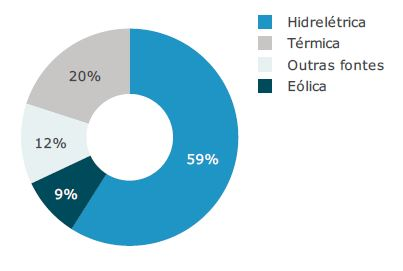
\includegraphics[width=0.6\linewidth]{imagens/cap01/Figura_1.1} 

}

\caption{Composição da matriz elétrica do Brasil em 2020. Fonte: MME (2020a)}\label{fig:01}
\end{figure}

\hypertarget{o-planejamento-do-setor-eluxe9trico}{%
\section{O planejamento do setor elétrico}\label{o-planejamento-do-setor-eluxe9trico}}

Reflexões, diretrizes e recomendações voltadas à expansão do setor elétrico podem ser encontradas em algumas análises produzidas no ambiente acadêmico (Gorayeb et al.~2019, Neri et al.~2019, Pinto \& Santos 2019, Agra Neto 2020), no setor produtivo (Oliveira et al.~2020) e em diversos documentos elaborados por agências governamentais, a exemplo do Planejamento Integrado de Recursos Energéticos - PIR, dos Planos Nacionais de Energia - PNE e os Planos Decenais de Expansão - PDE (MME 2020a, c).

O PIR é um estudo elaborado a partir de análises feitas no lado da carga e da geração, combinando as soluções encontradas que geram menores custos econômicos, sociais e ambientais para o país (Morales Udaeta 1997). O PNE avalia tendências na produção e no uso da energia e baliza as estratégias alternativas para expansão da oferta de energia nas próximas décadas. O PDE, elaborado anualmente pela Empresa de Pesquisa Energética (EPE), tem como objetivo indicar as perspectivas, sob a ótica do governo, da expansão do setor de energia no horizonte de 10 anos, numa visão integrada para os diversos recursos energéticos, visando ampliar a confiabilidade, reduzir os custos de produção e mitigar os impactos ambientais (MME 2020c).

Os dados, informações e diretrizes de todos esses estudos destinam-se a orientar as instâncias governamentais e sociedade civil e a subsidiar as empresas privadas interessadas na tomada de decisão e avaliação quanto à viabilidade de implantação de negócios no setor, assim como quanto à forma de condução desses processos. Alguns desses documentos contemplam diversas fontes, enquanto outros tratam especificamente da energia eólica, a exemplo de estudos alertando para o potencial de conflitos entre esse tipo de geração de energia e aspectos socioambientais (Gorayeb et al.~2019, Neri et al.~2019) e do relatório referente ao potencial de exploração da energia eólica \emph{offshore} no Brasil (MME 2020d).

\hypertarget{o-potencial-euxf3lico-brasileiro}{%
\section{O potencial eólico brasileiro}\label{o-potencial-euxf3lico-brasileiro}}

A exploração econômica da energia eólica depende da existência e disponibilidade de áreas com ocorrência de ventos regulares e constantes (velocidade média de 6,0 a 9,5 m/s), usualmente encontrados em áreas mais altas ou em algumas áreas baixas sem barreiras naturais ou artificiais (p.ex.: algumas áreas litorâneas).

Os principais aspectos relativos ao comportamento do vento considerados na avaliação do potencial eólico de uma dada região são sua intensidade, regularidade, sazonalidade e direção. Para a implantação de um empreendimento eólico, além de padrões gerais em nível regional e nacional, é necessário também analisar os fatores que influenciam o regime dos ventos em nível local, tais como relevo, rugosidade do solo e outros obstáculos (MME 2020a).

Os estudos de potencial eólico são fundamentais para o planejamento da implantação de empreendimentos eólicos no país. Um dos primeiros atlas do potencial eólico elaborados em escala nacional (Atlas do Potencial Eólico Brasileiro -- Amarante et al.~2001) estimou um potencial eólico para o país da ordem de 143,5 GW (Figura \ref{fig:02}), com as regiões Nordeste (75 GW - 52,3\%), Sudeste (29,7 GW - 20,7\%) e Sul (22,8 GW - 15,9\%) respondendo por 88,8\% desse total. O potencial estimado para as regiões Norte e Centro-Oeste foi de 12,8 GW (8,9\%) e 3,1 GW (2,2\%), respectivamente.

\begin{figure}[H]

{\centering 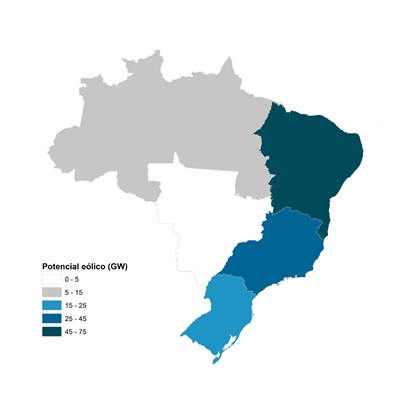
\includegraphics[width=0.7\linewidth]{imagens/cap01/Figura_1.2} 

}

\caption{Distribuição do potencial eólico das regiões do país. Fonte: Amarante et al. (2001)}\label{fig:02}
\end{figure}

De modo geral, as melhores áreas para aproveitamento eólico situam-se nas extremidades do sistema elétrico, distantes da geração hidrelétrica (Amarante et al.~2001). A região Nordeste apresenta as melhores condições do Brasil para o aproveitamento desse tipo de energia. Nessa região os regimes dos ventos são muito favoráveis e a vazão dos rios que atendem algumas usinas hidrelétricas é menor justamente quando ocorrem as melhores incidências de vento, demonstrando a complementaridade dessas fontes (MME 2007).

Uma versão mais recente de atlas de potencial eólico em escala nacional, com informações mais refinadas e modelagens com estimativas para diversas faixas de altura, contemplando inclusive aquelas condizentes com aerogeradores mais modernos (100, 120, 150 e 200 metros), pode ser consultada no sítio eletrônico \href{http://novoatlas.cepel.br/}{Atlas Eólico Brasileiro - Simulações 2013}. Além dessas informações em nível macro, diversos estados (SP, ES, BA, RN, CE, RS, PE, PB, AL, MG, PR e RJ) contam com estudos específicos, disponíveis no sítio eletrônico do \href{http://www.cresesb.cepel.br/}{Centro de Referências para as Energias Solar e Eólica Sérgio de S. Brito - CRESESB}.

\hypertarget{cenuxe1rio-da-energia-euxf3lica-no-pauxeds}{%
\section{Cenário da energia eólica no país}\label{cenuxe1rio-da-energia-euxf3lica-no-pauxeds}}

A energia elétrica de origem eólica é gerada por meio de aerogeradores ou turbinas eólicas. Esses equipamentos devem estar distribuídos em locais com abundância de ventos em condições favoráveis, devendo ainda estar ligados a estruturas associadas como subestações e linhas de transmissão, para escoamento da energia produzida.

Em geral, os aerogeradores são formados pelas serguintes partes:

\begin{itemize}
\item
  Pás: impulsionadas pela força dos ventos, geralmente em conjunto de três que formam ângulo de 120º, com formato aerodinâmico propício para o giro dentro do intervalo de mínimo e máximo de velocidade para a qual foi designada. Podem ser constituídas de plástico (PVC, PU ou PET), madeira balsa ou fibra de vidro.
\item
  Nacele (ou nave): abriga os componentes eletromecânicos (gerador, transformador, rotor, conversor, refrigerador, dentre outros). Situa-se junto ao eixo da hélice formada pelas pás, no qual a energia mecânica da rotação das pás é convertida em energia elétrica.
\item
  Torre: sustenta as pás e a nacele a uma altura variável, propícia para o recebimento dos ventos no local. Em geral, são feitas de aço e/ou concreto.
\end{itemize}

Um parque eólico consiste em um grupo de aerogeradores, distribuídos numa porção de espaço terrestre ou marítimo, gerenciados conjuntamente de forma a otimizar a geração de energia a partir da força dos ventos (transformação da energia cinética do vento em energia elétrica). Vários parques eólicos próximos ou contíguos podem formar um complexo eólico. \href{https://www.iberdrola.com/meio-ambiente/como-funcionam-parques-eolicos-onshore}{Veja aqui} um esquema do funcionamento de um aerogerador no interior de um parque eólico.

\hypertarget{parques-euxf3licos-onshore}{%
\subsection{\texorpdfstring{Parques eólicos \emph{onshore}}{Parques eólicos onshore}}\label{parques-euxf3licos-onshore}}

O primeiro aerogerador do Brasil foi instalado em 1992, em Fernando de Noronha, apenas para fins de pesquisa e, já no final dos anos 90, os primeiros parques eólicos comerciais \emph{onshore} (localizados no continente, em contraposição aos parques \emph{offshore}, situados em ambiente marinho) entraram em funcionamento no país (ANEEL 2003). Os aerogeradores da época eram bem menores que os atuais, com potência inferior a 1 MW (MME 2021). Na primeira metadade dos anos 2000, com apoio do Programa de Incentivo às Fontes Alternativas de Energia Elétrica - PROINFA, novos parques foram implantados. A partir de junho de 2006, a energia eólica gerada por esses parques (cerca de 3.500 GWh) passou a ser contabilizada no Sistema Interligado Nacional - SIN.

Nos anos seguintes, por meio de leilões e projetos do ACL, outros parques foram construídos e entraram em operação, e mais de 14 GW de potência passaram a abastecer o sistema elétrico brasileiro. Ao longo desse período, o avanço tecnológico possibilitou a produção e o uso de aerogeradores maiores, com torres mais altas e maior diâmetro dos rotores, com uma maior potência unitária e consequente aumento da produtividade.

Em fevereiro de 2021 o Brasil atingiu a marca de 695 parques eólicos e cerca de 8.300 aerogeradores distribuídos em seu território, totalizando aproximadamete 18 GW de capacidade instalada, considerando as usinas em pleno funcionamento e aquelas operando em testes autorizados pela ANEEL (CicloVivo 2021).

A participação da energia eólica na matriz elétrica brasileira saltou de 0,2\% em 2002 para 9\% em 2019, passando a ser a terceira fonte em capacidade instalada e a segunda dentre as renováveis. Estima-se que até 2029 esse número chegue a 17\%, atingindo cerca de 40 GW instalados (MME 2020b, 2021).

A Figura \ref{fig:03} apresenta a evolução da geração de energia eólica no Brasil de 2005 a 2020, em termos de potências instalada e acumulada por ano.

\begin{figure}[H]

{\centering 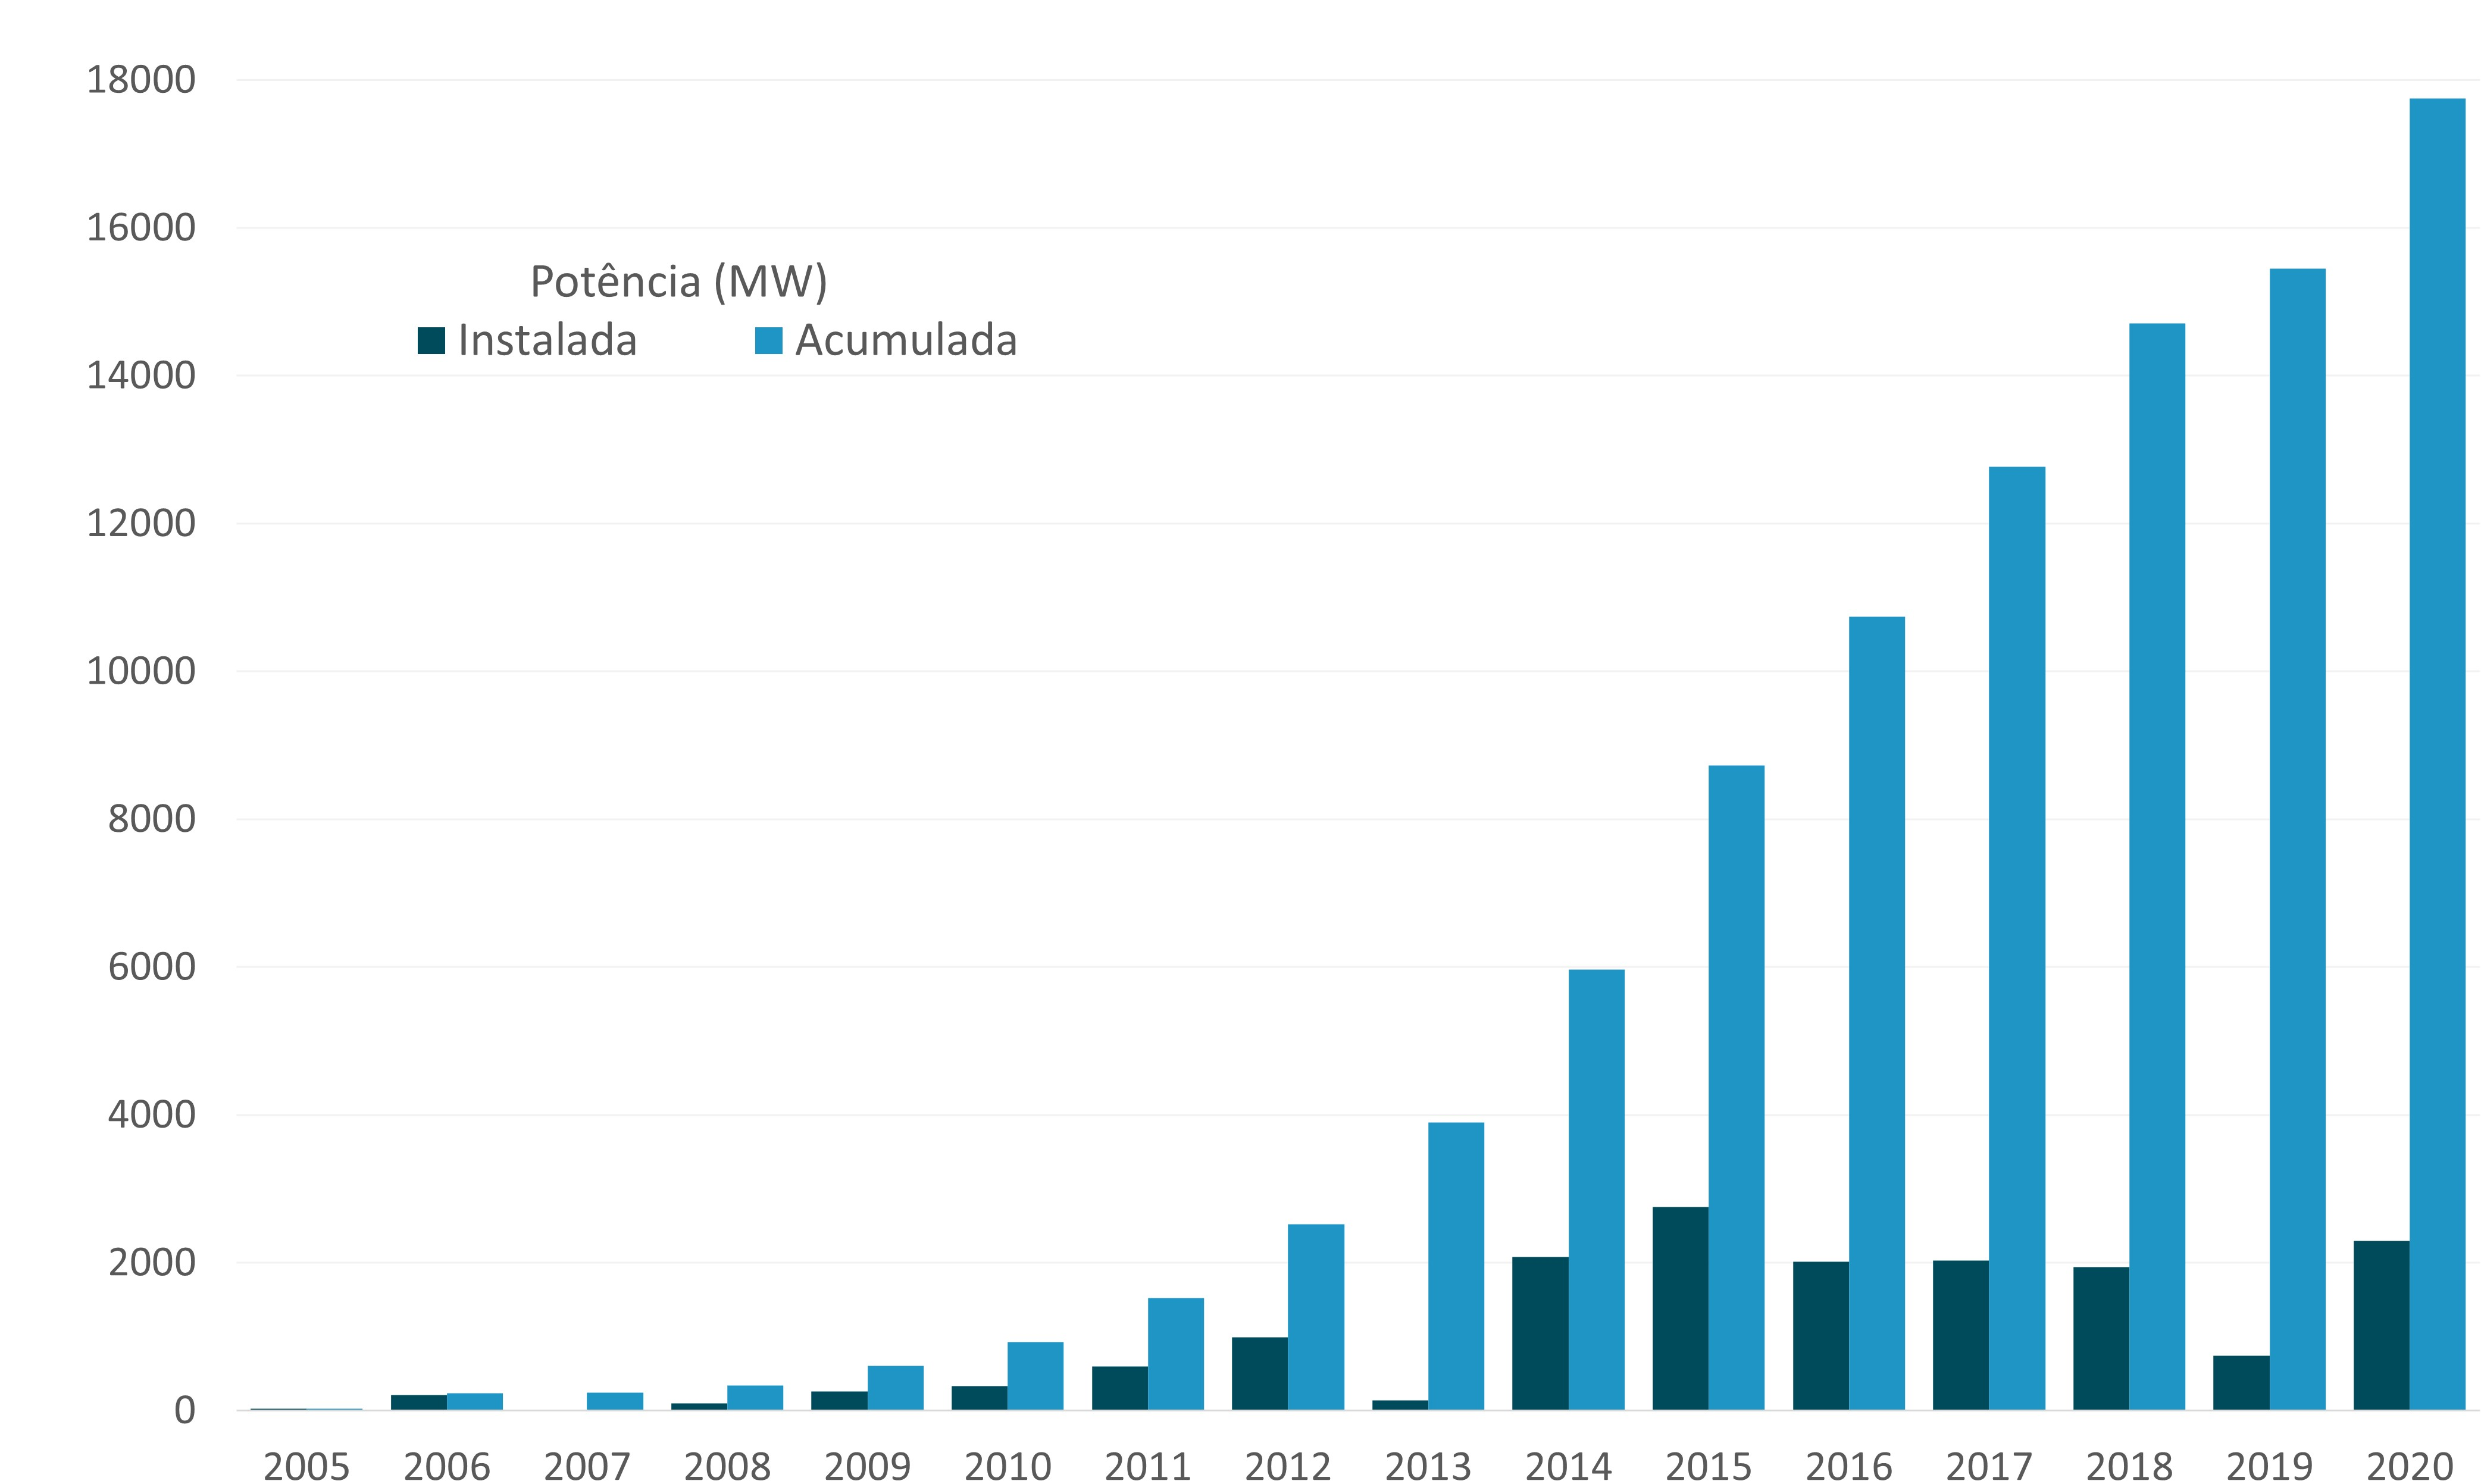
\includegraphics[width=0.8\linewidth]{imagens/cap01/Figura_1.3} 

}

\caption{Evolução da geração de energia eólica no Brasil de 2005 a 2020. Fonte: ABEEólica (2021)}\label{fig:03}
\end{figure}

Uma vez que as condições de vento e, consequentemente, o potencial eólico variam nas diferentes regiões do país, a distribuição espacial dos empreeendimentos eólicos tenderá a se correlacionar positivamente com o potencial eólico. Desta forma, apesar de atualmente os parques eólicos estarem distribuídos em 12 estados, há uma concentração de empreendimentos na regiões Nordeste e Sul, duas regiões com condições de vento bastante favoráveis à exploração comercial (Figura \ref{fig:04}).

\begin{figure}[H]

{\centering 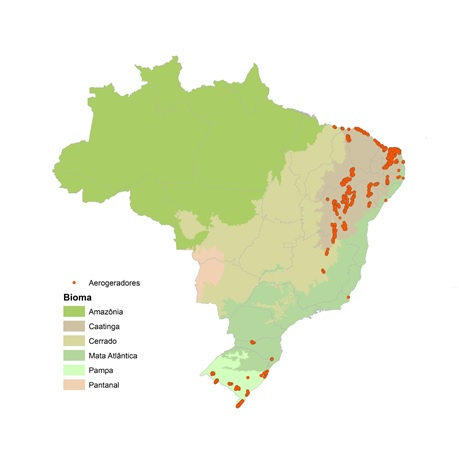
\includegraphics[width=0.7\linewidth]{imagens/cap01/Figura_1.4} 

}

\caption{Distribuição de parques eólicos (círculos laranjas) em atividade e planejados no território brasileiro. Notar o adensamento de empreendimentos nas regiões Nordeste e Sul, nos biomas Caatinga, Pampa e Mata Atlântica. Fonte: https://sigel.aneel.gov.br/}\label{fig:04}
\end{figure}

Além do mapeamento do potencial eólico, nos últimos anos \href{https://migratorysoaringbirds.birdlife.org/en/sensitivity-map\#gsc.tab=0}{Mapas de Sensibilidade} (Bright et al.~2008, McGuines et al.~2015, Morkūnė et al.~2020) ou ferramentas análogas (Neri et al.~2019) passaram a ser também empregados para subsidiar as tomadas de decisão acerca da localização e viabiliade de implantação desse tipo de empreendimento. O uso de tais ferramentas e abordagens possibilita que diferentes interesses da sociedade sejam considerados no momento de planejamento, favorecendo a identificação prévia de conflitos e a busca da adoção de medidas voltadas a compatibilizar diferentes visões sobre os usos a serem dados a uma determinada porção do território.

Atualmente, dentre os diversos estados que contam com empreendimentos eólicos, destacam-se o Rio Grande do Norte e a Bahia, com potência instalada na faixa do 5.000 MW (Figura \ref{fig:05}). Um segundo bloco importante é composto por estados com potência instalada de cerca de 2.000-2.500 MW (Piauí, Ceará e Rio Grande do Sul). Por fim, temos os estados com potência instalada de até 1000 MW (Pernambuco, Maranhão, Santa Catarina, Paraíba, Sergipe, Rio de Janeiro e Paraná).

\begin{figure}[H]

{\centering 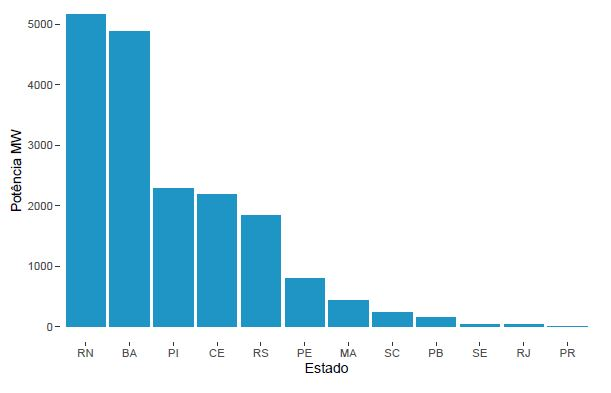
\includegraphics[width=0.8\linewidth]{imagens/cap01/Figura_1.5} 

}

\caption{Distribuição da potência instalada de geração de energia eólica por estado. Rio Grande do Norte e Bahia se destacam, com potência instalada na faixa dos 5000 MW. Fonte: ABEEólica (2021)}\label{fig:05}
\end{figure}

Considerando o número total de parques eólicos construídos, a Bahia já superou o Rio Grande do Norte (Figura \ref{fig:06}). Os dois estados juntos somam quase 50\% do total de parques eólicos instalados no país.

O \emph{ranking} também se altera no segundo bloco, com Ceará superando o Rio Grande do Sul e Piauí, em relação ao número total de parques instalados. Tais diferenças provavelmente estão relacionadas a variações nas tecnologias utilizadas em função da época de construção dos parques. Parques mais novos e mais modernos tendem a ser mais produtivos, de forma que um menor número de parques mais novos ou mesmo parques com um menor número de torres, podem, em determinadas condições, ser mais produtivos e gerar mais energia do que parques utilizando tecnologias mais antigas.

\begin{figure}[H]

{\centering 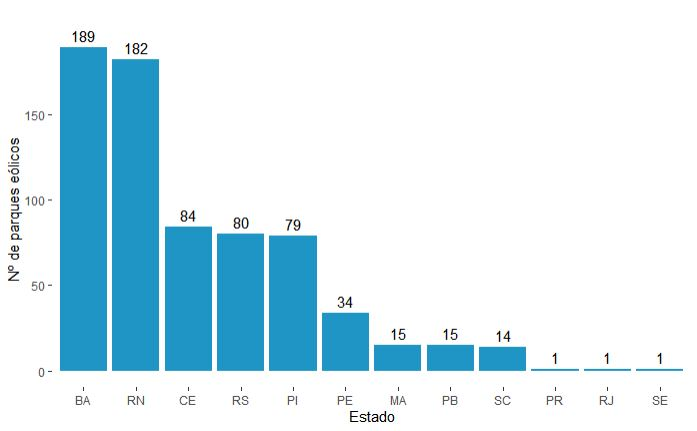
\includegraphics[width=0.8\linewidth]{imagens/cap01/Figura_1.6_1} 

}

\caption{Número de parques eólicos instalados por estado. Bahia e Rio Grande do Norte se destacam, com valores superiores a 150 parques. Fonte: ABEEólica (2021)}\label{fig:06}
\end{figure}

\hypertarget{parques-euxf3licos-offshore}{%
\subsection{\texorpdfstring{Parques eólicos \emph{offshore}}{Parques eólicos offshore}}\label{parques-euxf3licos-offshore}}

Atualmente o Brasil ainda não possui empreendimentos eólicos \emph{offshore} em funcionamento. O primeiro \href{https://www.ibama.gov.br/phocadownload/licenciamento/publicacoes/2020-11-TR_CEM.pdf}{Termo de Referência (TR) padrão para Estudo de Impacto Ambiental e Relatório de Impacto Ambiental (EIA/RIMA) de Complexos Eólicos Marítimos (\emph{Offshore})} foi lançado pelo Instituto Brasileiro do Meio Ambiente e dos Recursos Naturais (Ibama) em novembro de 2020. Este órgão licenciador federal conta, atualmente, com 45 processos referentes a projetos de empreendimentos eólicos \emph{offshore} em diferentes fases de licenciamento na costa das regiões Nordeste (20), Sudeste (13) e Sul (12), contemplando a instalação de 7.284 novos aerogeradores e um potencial de geração de 106,4 GW (M. Lauxen, com. pess. 2022).

O mapeamento preliminar do potencial eólico \emph{offshore} para as águas jurisdicionais brasileiras identificou áreas com ventos superiores a 7 m/s, abrindo novas perspectivas para a possível exploração desse recurso energético (MME 2020b). O potencial do país para a geração de energia eólica \emph{offshore} é muito grande, da ordem 700 GW em locais com profundidade de até 50 m (MME 2020d). Azevedo et al.~(2020) estimaram um potencial eólico \emph{offshore} ainda maior para a costa brasileira, de cerca de 3 TW e aproximadamente 15.000 TWh de produção média anual de eletricidade. Segundo esses autores, tais valores equivalem a cerca de 20 vezes a capacidade elétrica atualmente instalada no Brasil.

Algumas vantagens usualmente associadas à exploração da energia eólica \emph{offshore} incluem: as boas condições de vento, que no ambiente marinho costumam resultar em fatores de capacidade (eficiência) mais elevados; a maior proximidade dos centros de carga (consumo), uma vez que cerca de 80\% da população do país encontra-se nos grandes centros urbanos, localizados na região costeira; um menor impacto paisagístico, visto que os aerogeradores costumam ser localizados a uma certa distância da costa; um menor número de restrições e conflitos (quando se compara à modalidade \emph{onshore}) (MME 2020d).

Entretanto, o custo de exploração desse tipo de energia no Brasil é muito elevado quando comparado ao de outros países, em razão do alto custo de capital e dos desafios logísticos (Bosch et al.~2019). Informações mais refinadas sobre os potenciais de geração estimados são também ainda limitadas, sendo necessário um aprofundamento em relação a questões insuficientemente avaliadas, como usos conflitantes dos espaços marinhos e aspectos ambientais, tecnológicos e normativos.\\
Além disso, do ponto de vista operacional, uma vez que esse tipo de exploração tende a utilizar aerogeradores maiores e de maior capacidade nominal, desafios relacionados à logística de instalação e de manutenção, além da conexão para escoamento da energia ao continente e da capacidade de integração com os sistemas de transmissão e distribuição já existentes deverão ser enfrentados (adequação de rodovias e portos para apoio à instalação e manutenção das estruturas de geração e transmissão) (MME 2020c). Por fim, assim como no ambiente \emph{onshore}, as questões relacionadas ao descomissionamento precisam ser também consideradas no planejamento dos empreendimentos \emph{offshore} (MME 2021b).

Destacamos a importância de que os diferentes aspectos envolvidos na exploração \emph{offshore} sejam considerados de forma integrada e em escalas compatíveis para um planejamento adequado dessa modalidade de empreendimento eólico. Esses aspectos serão tratados de forma específica no capítulo 9 desta publicação.

\hypertarget{o-brasil-no-cenuxe1rio-mundial}{%
\section{O Brasil no cenário mundial}\label{o-brasil-no-cenuxe1rio-mundial}}

A Dinamarca foi pioneira no uso comercial da energia eólica, ainda na década de 70 (ANEEL 2003), sendo rapidamente seguida por outros países europeus como Holanda, Bélgica, Suécia, Reino Unido e Alemanha. Posteriormente, impulsionados pelo aumento da demanda por energia em razão do crescimento econômico e por crises na oferta de petróleo, países como Estados Unidos, Espanha, Portugal e China também passaram a investir de forma significativa na exploração desse tipo de energia (Oliveira et al.~2020).

O ano de 2020 foi o melhor ano da história para a indústria eólica em termos globais, com um total de 93 GW de nova capacidade instalada (GWEC 2021). O recorde de 2020 deu-se devido ao crescimento acentuado na China e nos Estados Unidos, os dois maiores mercados mundiais de energia eólica que, juntos, foram responsáveis por cerca de 75\% da quantidade instalada em 2020. Atualmente, a capacidade instalada mundial soma 743 GW (707 GW - 95\% \emph{onshore} e 36 GW - 5\% \emph{offshore}), ajudando a evitar a emissão de mais de 1,1 bilhão de toneladas de CO\textsubscript{2} para a atmosfera (GWEC 2021).

A Dinamarca foi também o primeiro país a instalar um parque eólico \emph{offshore}, ainda em 1991. Atualmente há cerca de uma centena de parques eólicos \emph{offshore} distribuídos pelo mundo, todos eles no hemisfério Norte (GWEC 2021). Os cerca de 36 GW de capacidade total instalada estão distribuídos, em grande parte, no Reino Unido, Alemanha, China, Dinamarca e Bélgica, enquanto uma parcela menor dessa geração é realizada por um grupo de países com pequena produção.

O Brasil tem um grande potencial de exploração e, em pouco mais de duas décadas, teve um avanço muito significativo na sua capacidade instalada. Em 2019, o país subiu uma posição no \emph{ranking} e passou a ocupar a 7ª posição no mundo em termos de potência instalada de energia eólica (Figura \ref{fig:07}). Apesar do bom desempenho, encontra-se ainda bem distante de países também continentais como Estados Unidos e China. Tais países têm uma alta demanda enérgica, seja pelo elevado padrão de consumo de sua população ou pela alta densidade populacional, além de um contínuo crescimento econômico que depende de sua capacidade de geração de energia.

\begin{figure}[H]

{\centering 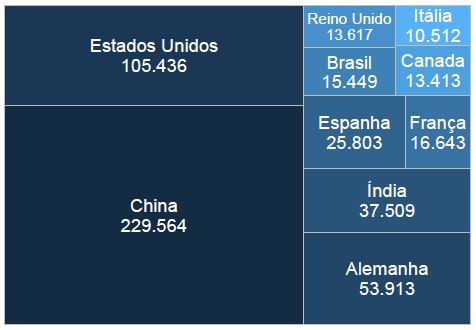
\includegraphics[width=0.7\linewidth]{imagens/cap01/Figura_1.7} 

}

\caption{Países com maior capacidade de geração de energia eólica. Os valores indicam o potencial instalado em MW. Fonte: GWEC (2021)}\label{fig:07}
\end{figure}

\hypertarget{impactos-da-gerauxe7uxe3o-de-energia-euxf3lica}{%
\section{Impactos da geração de energia eólica}\label{impactos-da-gerauxe7uxe3o-de-energia-euxf3lica}}

Assim como as demais formas de geração de energia, a energia eólica possui diversos aspectos positivos que favorecem e estimulam sua implementação, mas também alguns aspectos negativos e limitações (Gorayeb et al.~2019, Neri et al.~2019), como a irregularidade na geração e o menor controle, que podem, inclusive, comprometer a expansão de sua utilização em algumas situações específicas.

De modo geral, quando comparada às outras fontes de geração (especialmente aos combustíveis fósseis), a energia de origem eólica é considerada uma energia limpa, renovável, segura e inesgotável. Ainda que partes de sua cadeia produtiva não estejam livres da geração de impactos, sua produção em si gera relativamente poucos resíduos e não há emissão de radiações, nem de gases tóxicos ou que contribuam para as mudanças climáticas. As instalações eólicas permitem a continuidade da maior parte das atividades agrícolas e pecuárias, que podem ser desenvolvidas concomitantemente nos locais de exploração e as áreas onde os parques são instalados podem ser recuperadas com relativa facilidade após a vida útil do empreendimento. Os impactos ambientais são menores e os riscos de acidentes com impactos socioambientais significativos são muito baixos. Além disso, a energia produzida é comparativamente mais barata (CCEE 2021) e há potencial de geração de emprego e renda e aquecimento da economia local (Oliveira et al.~2020), especialmente na fase de implantação, ainda que de forma temporária.

Por sua vez, há também evidências de alguns impactos negativos (Dai et al.~2015). Bastante documentados são os impactos sobre a fauna, principalmente morcegos e aves (Choi et al.~2020). Há descrições de impactos sobre a paisagem (poluição visual) e sobre ambientes sensíveis (dunas e montanhas), além de impactos negativos sobre processos de criação ou sobre áreas protegidas já estabelecidas (Neri et al.~2019). Podem ocorrer perda e fragmentação de \emph{habitat}, decorrentes da abertura de vias de acesso e instalação de estruturas associadas (linhas de transmissão e subestações), além de conflitos com moradores locais (pescadores, quilombolas, indígenas) em razão de sobreposição e restrição de usos (acessos para pesca, turismo), além de eventuais problemas de saúde associados à emissão de ruído pelas pás das torres (Gorayeb et al.~2019).

Especificamente no caso de empreendimentos \emph{offshore}, em relação às questões socioambientais destacam-se potenciais conflitos e restrições relacionadas à sobreposição com áreas legalmente protegidas, efeitos na paisagem, impactos sobre atividades de turismo e recreação, conflitos com áreas de pesca tradicional e artesanal, sobreposição com rotas migratórias (mamíferos, aves, répteis), impactos sonoros (especialmente durante a construção) e alteração de campo eletromagnético (Bailey et al.~2014).

Esse conjunto de impactos, tanto positivos quanto negativos, não é exaustivo, sendo aqui apresentado apenas de forma geral e superficial, com vistas a fornecer uma visão panorâmica de alguns aspectos que devem ser considerados, ponderados e conciliados nas etapas de planejamento e licenciamento ambiental para se assegurar um processo adequado de implantação dos empreendimentos eólicos. Impactos não mencionados poderão se aplicar a casos particulares e uma discussão detalhada sobre aqueles mais conhecidos e recorrentes será apresentada em capítulo específico desse relatório.

A quantidade e intensidade dos impactos podem ainda ser muito influenciadas pela localização do empreendimento. Analisando a distribuição de parques eólicos instalados até 2018 em 4 estados (Ceará, Rio Grande do Norte, Bahia e Rio Grande do Sul), perfazendo 80\% da capacidade total instalada no país, Turkovska et al.~(2021) constataram que 50\% dos parques encontram-se em áreas com cobertura vegetal nativa, 20\% sobre dunas e apenas 30\% em áreas antropizadas.

Destacamos, portanto, que cabe a todos os atores envolvidos nos processos de planejamento dos novos parques eólicos procurar otimizar sua qualidade e efetividade adotando medidas que intensifiquem os benefícios e eliminem ou minimizem as perdas para a sociedade, em especial, sobre aqueles elementos da biodiversidade mais sensíveis e grupos sociais mais vulneráveis, e que estejam mais próximos dos locais de geração de energia.

\hypertarget{perspectivas-para-o-futuro}{%
\section{Perspectivas para o futuro}\label{perspectivas-para-o-futuro}}

Análises de cenários futuros indicam o crescimento de todas as fontes da matriz elétrica brasileira, porém com um crescimento relativo mais acentuado da energia eólica (MME 2020b). Espera-se uma redução da participação das usinas hidrelétricas devido aos desafios socioambientais e econômicos enfrentados por esse tipo de geração, tendo em vista que os recursos hídricos com potencial de uso encontram-se em locais ambientalmente mais frágeis e distantes dos locais de maior consumo. Já a tendência de crescimento do setor de energia eólica deverá ser mantida.

A energia elétrica de origem eólica é a que tem maior potencial de crescimento nos próximos anos, com vantagens econômicas e ambientais, mas com maiores desafios operacionais por ser uma fonte variável e não controlável.

Considerando os mapeamentos do potencial eólico do país, tanto em larga escala quanto nos estudos estaduais, há ainda uma ampla capacidade de expansão do setor em médio e longo prazos, ambos \emph{onshore} e \emph{offshore}. O aprimoramento tecnológico e o uso de aerogeradores mais altos e de maior potência, com aumento da produtividade por unidade, deverá favorecer esse crescimento e a exploração desse potencial (Além da Energia 2021). Esse avanço também deverá ser favorecido pela pressão internacional pelo uso de energias mais limpas para redução da emissão de carbono.

A ABEEólica prevê que a capacidade instalada alcance 28 GW até 2024 (Canal Energia 2021). Estima-se que em 2030 a energia hidrelétrica responderá por 49\% da matriz elétrica, ao tempo que a energia eólica responderá por 14\% (33 GW) dos 236 GW previstos para a matriz (MME 2020a - Figura \ref{fig:08}).

\begin{figure}[H]

{\centering 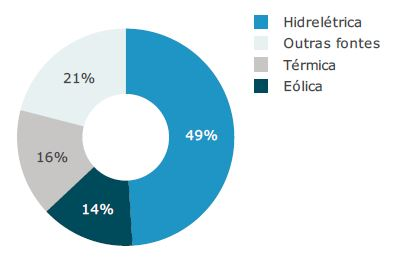
\includegraphics[width=0.6\linewidth]{imagens/cap01/Figura_1.8} 

}

\caption{Previsão da composição da matriz elétrica do Brasil em 2030. Fonte: MME (2020a)}\label{fig:08}
\end{figure}

Mesmo com sua redução em termos relativos, a energia de origem hidráulica continuará cumprindo um importante papel em assegurar a estabilidade do sistema, visto haver uma complementariedade sazonal entre essas fontes. Deverá se contar ainda, nesse papel, com a participação das termelétricas, prevendo-se também a modernização de parte dessas usinas para ganho de eficiência. O sistema tenderá a manter uma matriz com fontes predominantemente renováveis, não emissoras de gases de efeito estufa, principalmente devido à ampliação das fontes de energia eólica e solar (MME 2020b).

Há previsão de investimentos para expansão das linhas de transmissão e subestações no sistema para dar suporte ao escoamento da energia gerada por diversas fontes nas diferentes regiões do país, com ênfase nas áreas norte, leste e sul da região Nordeste, além de obras de expansão na região Sul (MME 2020c). Está também prevista uma ampliação de cerca de 30\% nas linhas de transmissão num período de 10 anos, passando de 154 mil km em 2019 para 203 mil km em 2029 (implantação de 49 mil km de linhas - MME 2020c).

Em termos regionais/estaduais, há perspectivas de que o estado da Bahia poderá assumir a liderança na produção e comercialização em razão de vantagens competitivas devido a aspectos geográficos, logísticos, maior avanço no dimensionamento da capacidade de fornecimento (produção de Atlas Eólico para o estado), disponibilidade de linhas de transmissão e gestão ágil dos projetos (Agra Neto et al.~2020).

Cabe ressaltar que a expansão observada no Brasil nos últimos anos refere-se ainda somente a projetos \emph{onshore}. No contexto global, regiões \emph{offshore} representam a última fronteira para o desenvolvimento da energia eólica, com aumento expressivo na exploração dessa fonte nessas regiões em alguns países como China e Estados Unidos. O mapeamento preliminar do potencial eólico \emph{offshore} no Brasil indica ser possível um crescimento similar no país, a partir do sucesso das primeiras iniciativas de exploração dessa modalidade (MME 2020b).

\hypertarget{avanuxe7os-tecnoluxf3gicos}{%
\subsection{Avanços tecnológicos}\label{avanuxe7os-tecnoluxf3gicos}}

Os custos relativos à implantação dos projetos eólicos tendem a se reduzir ao longo do tempo, resultado dos avanços tecnológicos como o aumento da altura das torres, a evolução do material de composição das pás, a ampliação de sua área de varredura e o aumento da potência nominal dos aerogeradores. A altura das torres dos parques eólicos \emph{onshore} tem aumentado progressivamente, atingindo a média de 112 m em 2019 (MME 2020b). Em relação às pás, novos materiais como fibras de carbono ou fibras híbridas de vidro e carbono poderão vir a ser empregadas na confecção dessas estruturas para redução de peso (MME 2020b). A tendência de aumento do tamanho de torres e pás tende a ampliar o fator de capacidade sob determinadas condições de vento. Porém, aerogeradores maiores exigirão adequações e inovações para possibilitar a logística de armazenamento e transporte de suas estruturas (MME 2020b).

Na modalidade \emph{offshore}, inovações tecnológicas como o uso de fundações flutuantes estão sendo estudadas para permitir o suporte de aerogeradores e a exploração em áreas mais profundas, assim como o uso de aerogeradores maiores, com vistas à redução de custos (MME 2020c). O emprego de de grandes aerogeradores, com diâmetro do rotor médio de 150 m e potência nominal superior a 6 MW, é uma das principais características dos projetos eólicos \emph{offshore} e alguns equipamentos mais modernos podem alcançar até 15 MW (MME 2020b, Além da Energia 2021, Lauxen 2021).

Os impactos das alterações estruturais ou operacionais decorrentes dos avanços tecnológicos dos parques eólicos sobre aves e morcegos também precisarão ser avaliados. O uso de aerogeradores mais altos e com pás maiores, por exemplo, pode ampliar o impacto sobre algumas espécies e implicar a necessidade de alterações nos protocolos de monitoramento (Choi et al.~2020). Por outro lado, a maior produtividade por unidade pode, em tese, também vir a diminuir o número de aerogeradores por planta, com efeitos na redução tanto do número de torres quanto na extensão do território ocupada, de forma que impactos positivos e negativos podem se contrabalançar. Questões desse tipo precisarão ser identificadas e investigadas.

\hypertarget{alguns-desafios}{%
\subsection{Alguns desafios}\label{alguns-desafios}}

O crescimento e a diversificação da matriz elétrica no Brasil, com a significativa ampliação do uso da energia eólica, implicam o enfrentamento e a superação de uma série de desafios. As agências do Sistema Elétrico Nacional precisam se preparar para lidar com uma matriz com grande percentual de geração variável e menor capacidade de controle.

Nas etapas de planejamento deve-se buscar incorporar nos estudos socioambientais prévios análises integradas que considerem o aumento da complexidade e os impactos cumulativos ou sinérgicos de diversos empreendimentos localizados próximos. Em que pesem as dificuldades metodológicas e de acesso e compartilhamento de dados e informações entre empreendimentos, a consideração desses potenciais efeitos nos estudos exigidos durante o licenciamento ambiental pode contribuir para a identificação de impactos ambientais relevantes e possibilitar a indicação de medidas integradas de controle ou mitigação para projetos implantados numa mesma região. Num país megadiverso como o Brasil, a publicação e o compartilhamento de dados de monitoramento e avaliação dos impactos dos empreendimentos sobre a biodiversidade, em especial sobre aves e morcegos, é de suma importância para aprimorar e assegurar maior qualidade técnica ao processo de ampliação do uso da energia eólica em nosso território.

A seleção adequada de locais para a instalação de empreendimentos é uma questão central, uma vez que a instalação de parques fora ou com pouca sobreposição com áreas sensíveis em termos socioambientais por si só, sejam elas áreas legalmente protegidas ou não, já reduz significativamente os riscos e os impactos negativos dos parques eólicos. Com base na constatação de que 70\% dos parques eólicos instalados no país encontram-se em áreas com vegetação nativa ou dunas, Turkovska et al.~(2021) argumentam pela instalação de empreendimentos em áreas já antropizadas, com condições de vento apropriadas. Marinho et al.~(2021) apresentam uma reflexão ampla do potencial impacto dos parques eólicos sobre áreas prioritárias para conservação na Caatinga.

Num cenário ideal, a expansão dessa atividade deveria basear-se no planejamento estratégico em larga escala, em nível de paisagem, empregando bases de dados espaciais com informações robustas de diferentes temas e considerando diferentes interesses e usos potenciais da região considerada. O uso de mapas de sensibilidade e ferramentas análogas é extremamente recomendável como um elemento complementar ou associado aos processos de licenciamento ambiental, e seus benefícios serão tanto maiores quanto antes ele ocorrer nas etapas de planejamento.

Desafios relacionados à logística, integração entre geração e transmissão/distribuição, normatização de processos e regulamentação de ações de descomissionamento já vêm sendo discutidos em maior ou menor profundidade em documentos de planejamento governamentais (MME 2020b).

É consenso que a implantação de novos parques eólicos exigirá o aprimoramento da logística de transporte dos equipamentos (tendo em vista a tendência de aumento de seu tamanho e peso). Na modalidade \emph{onshore} os desafios são as estradas e rodovias que, principalmente em áreas rurais e áreas urbanas adensadas, em geral, não apresentam condições apropriadas para o transporte das estruturas desse tipo de empreendimento. Já para a exploração \emph{offshore} existem as limitações da infraestrutura portuária e de navegação, além de eventuais restrições ambientais, de navegação ou de outros usos conflitantes (MME 2020c).

Outro ponto importante consiste na necessidade de integração do planejamento e ações de expansão da geração eólica com o planejamento e implantação da transmissão. O recurso eólico possui alta variabilidade horária e sua integração em larga escala no SIN implica contínuo redimensionamento da Rede Básica, especialmente na região Nordeste, que é onde se encontra a maior parte do potencial eólico brasileiro (MME 2020b). Os maiores centros de carga estão nas regiões Sul e Sudeste, ampliando a necessidade de ajustes para garantir os intercâmbios elétricos entre os subsistemas. Os impactos socioambientais da ampliação dessas estruturas de escoamento da energia gerada também deverão ser considerados. O avanço tecnológico previsto para os aerogeradores e a possibilidade de desenvolvimento de plantas de geração híbridas eólico-solar e de projetos eólicos \emph{offshore} poderão representar novos desafios para o planejamento da expansão da transmissão (MME 2020b).

A elaboração ou adequação de normativas para dar suporte e segurança jurídica ao desenvolvimento do setor é também fundamental. Faz-se necessário um arcabouço legal e regulatório que contemple os diferentes aspectos do setor (ambiental, social, comercial etc.). No caso da exploração \emph{offshore}, por exemplo, há lacunas na legislação marítima vigente, que não contempla ainda os efeitos desse tipo de intervenção no ambiente.

O setor precisará avançar na elaboração e execução de protocolos voltados à repotenciação e descomissionamento dos parques eólicos. Serão necessárias normas para descomissionamento e análise da viabilidade de repotenciação, além de avaliação dos impactos no sistema (atendimento da demanda e flexibilização). Segundo a EPE (MME 2021), até 2030, mais de 50 parques alcançarão a faixa dos 20 anos de operação (vida útil média dos equipamentos desses empreendimentos), representando mais de 600 aerogeradores e de 940 MW de potência. Assim, evidencia-se a importância de se discutir possíveis ações após esse período, sejam elas de manutenção, modernização ou descomissionamento dos parques eólicos instalados (MME 2021).

Ressaltamos que, nos empreendimentos futuros, dois aspectos devem merecer especial atenção: a) o uso de estudos qualificados e participação de diferentes atores nas etapas de planejamento para definição da localização dos parques, buscando-se evitar ou reduzir sua sobreposição com áreas socioambientalmente sensíveis e b) a implementação de programas de monitoramento de médio ou longo prazos, que considerem os períodos pré e pós-instalação dos parques. Alguns estudos de impactos de curta duração têm mostrado respostas conflitantes, espécie-específicas ou bastante dependentes das particularidades locais, dificultando o estabelecimento de generalizações capazes de orientar adequadamente a tomada de decisão pelas instâncias pertinentes (Shöll \& Nopp-Mayr 2021).

Por fim, entendemos que parte da sociedade já reconhece a importância e necessidade de conciliarmos a expansão do uso da energia eólica e consequente redução da emissão de gases do efeito estufa com a proteção da biodiversidade e seus serviços ambientais (ver Neri et al.~2019, Marinho et al.~2021). Assegurar a transparência e a participação qualificada de diferentes segmentos nos processos de planejamento e tomada de decisão sobre o tema, considerando de forma equilibrada aspectos econômicos, políticos, ambientais e sociais, poderá transformar conflitos reais ou potenciais em oportunidades. A participação da energia eólica na matriz elétrica brasileira é crescente e bem-vinda, mas seu crescimento no país deve estar baseado num planejamento adequado que otimize seus benefícios a partir da ponderação dos diferentes interesses da sociedade brasileira.

\newpage

\hypertarget{referuxeancias-bibliogruxe1ficas}{%
\section{Referências bibliográficas}\label{referuxeancias-bibliogruxe1ficas}}

ABEEólica (Associação Brasileira de Energia Eólica). 2021. Boletim Anual Dados 2020. Disponível em: \url{http://abeeolica.org.br/wp-content/uploads/2021/06/PT_Boletim-Anual-de-Gera\%C3\%A7\%C3\%A3o_2020.pdf} Acesso em: {[}14/09/2021{]}.

Agra Neto, J., Queiroz, F.C.B.P., Queiroz, J.V., Lima, N.C., Silva, C.L. 2020. Evolução e perspectivas do setor eólico no Brasil: análise dos principais estados produtores. Revista em Agronegócio e Meio Ambiente 13(4): 1409-1432. \url{https://doi.org/10.17765/2176-9168.2020v13n4p1409-1432}

Amarante, O.A.C., Brower, M., Zack, J., Sá, A.L. 2001. Atlas do potencial eólico brasileiro. Disponível em: \url{http://www.cresesb.cepel.br/publicacoes/download/atlas_eolico/Atlas\%20do\%20Potencial\%20Eolico\%20Brasileiro.pdf} Acesso em: {[}07/05/2021{]}.

ANACE (Associação Nacional dos Consumidores de Energia). 2021. Organização institucional do setor elétrico. Disponível em: \url{http://www.anacebrasil.org.br/energia/setor-eletrico/\#1484923187411-e467cd37-ff31} Acesso em: {[}07/05/2021{]}.

ANEEL (Agência Nacional de Energia Elétrica). 2003. Atlas de energia elétrica do Brasil. Disponível em: \url{http://www2.Aneel.gov.br/aplicacoes/atlas/pdf/06-energia_eolica(3).pdf} Acesso em: {[}07/05/2021{]}.

Azevedo, S.S.P., Pereira Jr, A.O., Silva, N.F., Araújo, R.S.B., Carlos Jr, A.A. 2020. Assessment of Offshore Wind Power Potential along the Brazilian Coast. Energies 13(10): 2557. \url{https://doi.org/10.3390/en13102557}

Bailey, H., Brookes, K.L., Thompson, P.M. 2014. Assessing environmental impacts of offshore wind farms: lessons learned and recommendations for the future. Aquatic Biosystems 10(8): 1-13. \url{https://doi.org/10.1186/2046-9063-10-8}

Bosch, J., Staffell, I., Hawkes, A.D. 2019. Global levelised cost of electricity from offshore wind. Energy 189: 116357. \url{https://doi.org/10.1016/j.energy.2019.116357}

Bright, J., Langston, R., Bullman, R., Evans, R., Gardner, S., Pearce-higgins, J. 2008. Map of bird sensitivities to wind farms in Scotland: a tool to aid planning and conservation. Biological Conservation 141(9): 2342--2356. \url{https://doi.org/10.1016/j.biocon.2008.06.029}

CCEE (Câmara de Comercialização de Energia Elétrica). 2021. Custo final da energia eólica é o mais baixo entre as fontes renováveis. Disponível em: \url{https://www.ccee.org.br/portal/faces/pages_publico/noticias-opiniao/noticias/noticialeitura?contentid=CCEE_656850\&_adf.ctrl-state=olewrvrsm_1\&_afrLoop=23076559182296\#!\%40\%40\%3Fcontentid\%3DCCEE_656850\%26_afrLoop\%3D23076559182296\%26_adf.ctrl-state\%3Dolewrvrsm_5} Acesso em: {[}07/05/2021{]}.

Choi, D.Y., Wittig, T.W., Kluever, B.M. 2020. An evaluation of bird and bat mortality at wind turbines in the Northeastern United States. PLoS ONE 15(8): e0238034. \url{https://doi.org/10.1371/journal.pone.0238034}

Ciclovivo. 2021. Energia eólica começa 2021 em alta no Brasil. Disponível em: \url{https://ciclovivo.com.br/planeta/energia/energia-eolica-comeca-2021-em-alta-no-brasil/} Acesso em: {[}07/05/2021{]}.

Dai, K., Bergot, A., Liang, C., Xiang, W.-N., Huang, Z. 2015. Environmental issues associated with wind energy -- a review. Renewable Energy 75: 911--921. \url{https://doi.org/10.1016/j.renene.2014.10.074}

Gorayeb, A., Brannstrom, C., Meireles, A.J.A. (org.) 2019. Impactos socioambientais da implantação dos parques de energia eólica no Brasil. Edições UFC. Fortaleza. Disponível em: \url{http://www.observatoriodaenergiaeolica.ufc.br/wp-content/uploads/2019/07/livro_web.pdf} Acesso em: {[}07/05/2021{]}.

GWEC (Global Wind Energy Council). 2021. Global Wind Report 2021. Disponível em: \url{https://gwec.net/global-wind-report-2021} Acesso em: {[}07/05/2021{]}.

IBGE (Instituto Brasileiro de Geografia e Estatística). 2021. População do Brasil. Disponível em \url{https://www.ibge.gov.br/apps/populacao/projecao/box_popclock.php} Acesso em: {[}07/05/2021{]}.

McGuinness, S., Muldoon, C., Tierney, N., Cummins, S., Murray, A., Egan, S., Crowe, O. 2015. Bird Sensitivity Mapping for Wind Energy Developments and Associated Infrastructure in the Republic of Ireland. BirdWatch Ireland. Kilcoole. Wicklow. Disponível em: \url{https://tethys.pnnl.gov/sites/default/files/publications/McGuinness-2015.pdf} Acesso em: {[}07/05/2021{]}.

MME (Ministério de Minas e Energia). 2007. Plano Nacional de Energia 2030. Empresa de Pesquisa Energética. Brasília. Disponível em: \url{https://www.epe.gov.br/pt/publicacoes-dados-abertos/publicacoes/Plano-Nacional-de-Energia-PNE-2030} Acesso em: {[}07/05/2021{]}.

MME (Ministério de Minas e Energia). 2019. Consumo anual de energia elétrica por classe (nacional). Empresa de Pesquisa Energética. Brasília. Disponível em: \url{https://www.epe.gov.br/pt/publicacoes-dados-abertos/publicacoes/consumo-de-energia-eletrica/consumo-anual-de-energia-eletrica-por-classe-(nacional)} Acesso em: {[}07/05/2021{]}.

MME (Ministério de Minas e Energia). 2020a. Plano Decenal de Expansão de Energia 2030. Empresa de Pesquisa Energética. Brasília. Disponível em: \url{https://www.epe.gov.br/pt/publicacoes-dados-abertos/publicacoes/plano-decenal-de-expansao-de-energia-2030} Acesso em: {[}07/05/2021{]}.

MME (Ministério de Minas e Energia). 2020b. Plano Nacional de Energia 2050. Empresa de Pesquisa Energética. Brasília. Disponível em: \url{https://www.epe.gov.br/pt/publicacoes-dados-abertos/publicacoes/Plano-Nacional-de-Energia-2050} Acesso em: {[}07/05/2021{]}.

MME (Ministério de Minas e Energia). 2020c. Roadmap Eólica Offshore Brasil: perspectivas e caminhos para a energia eólica marítima. NT-EPE-PR-001/2020-r2. Empresa de Pesquisa Energética. Brasília. Disponível em: \url{https://www.epe.gov.br/sites-pt/publicacoes-dados-abertos/publicacoes/PublicacoesArquivos/publicacao-456/Roadmap_Eolica_Offshore_EPE_versao_R2.pdf} Acesso em: {[}07/05/2021{]}.

MME (Ministério de Minas e Energia). 2020d. Plano Decenal de Expansão de Energia 2029. Empresa de Pesquisa Energética. Brasília. \url{https://www.epe.gov.br/pt/publicacoes-dados-abertos/publicacoes/plano-decenal-de-expansao-de-energia-2029} Acesso em: {[}07/05/2021{]}.

MME (Ministério de Minas e Energia). 2021a. Modernização do Setor Elétrico. Disponível em: \url{https://www.gov.br/mme/pt-br/assuntos/secretarias/secretaria-executiva/modernizacao-do-setor-eletrico/gt-modernizacao} Acesso em: {[}10/11/2021{]}.

MME (Ministério de Minas e Energia). 2021b. Empreendimentos eólicos ao fim da vida útil: situação atual e alternativas futuras. EPE-DEE-NT-012/2021. Empresa de Pesquisa Energética. Brasília. Disponível em: \url{https://www.epe.gov.br/sites-pt/publicacoes-dados-abertos/publicacoes/PublicacoesArquivos/publicacao-563/NT-EPE-DEE-012-2021.pdf} Acesso em: {[}07/05/2021{]}.

Morales Udaeta, M.E. 1997. Planejamento Integrado de Recursos Energéticos -- PIR - para o setor elétrico (pensando o desenvolvimento sustentável). Tese de Doutorado. Universidade de São Paulo. São Paulo. \url{Doi:10.11606/T.3.1997.tde-09082001-113018}.

Morkūnė, R., Marčiukaitis, M., Jurkin, V., Gecevičius, G., Morkūnas, J., Raudonikis, L. et al.~2020. Wind energy development and wildlife conservation in Lithuania: A mapping tool for conflict assessment. PLoS ONE 15(1): e0227735. \url{https://doi.org/10.1371/journal.pone.0227735}

Neri, M., Jameli, D., Bernard, E., Melo, F.P.L. 2019. Green versus green? Adverting potential conflicts between wind power generation and biodiversity conservation in Brazil. Perspectives in Ecology and Conservation 17(3): 131--135. \url{https://doi.org/10.1016/j.pecon.2019.08.004}

Oliveira, G., Curi, A.Z., Felini, P.S., Ficarelli, T.R.A. 2020. Impactos socioeconômicos e ambientais da geração de energia eólica no Brasil. Relatório. GO Associados. São Paulo. Disponível em: \url{https://epbr.com.br/wp-content/uploads/2021/02/ABEEolica_GO-Associados-V.-Final.pdf} Acesso em: {[}07/05/2021{]}.

Pinto, R.J., Santos, V.M.L. 2019. Energia eólica no Brasil: evolução, desafios e perspectivas. Journal on Innovation and Sustainability 10(1): 124-142. \url{http://dx.doi.org/10.24212/2179-3565.2019v10i1p124-142}.

Schöll, E.M., Nopp-Mayr, U. 2021. Impact of wind power plants on mammalian and avian wildlife species in shrub- and woodlands. Biological Conservation 256: 109037. \url{https://doi.org/10.1016/j.biocon.2021.109037}

Turkovska, O., Castro, G., Klingler, M., Nitsch, F., Regner, P., Soterroni, A. C., Schmidt, J. 2021. Land-use impacts of Brazilian wind power expansion. Environmental Research Letters 16(2): 024010. DOI: 10.13140/RG.2.2.29794.76480

\hypertarget{cap2}{%
\chapter{Atualização da lista de aves migratórias do Brasil}\label{cap2}}

\textbf{Marina Somenzari, Natália da Mata Luchetti \& Priscilla Prudente do Amaral}

\emph{Centro Nacional de Pesquisa e Conservação de Aves Silvestres -- CEMAVE}\\
\emph{Instituto Chico Mendes de Conservação da Biodiversidade -- ICMBio}\\
\emph{Floresta Nacional da Restinga de Cabedelo}\\
\emph{BR-230 Km 10}\\
\emph{58108-012 Cabedelo, PB}

A migração pode ser definida como movimentos cíclicos e sazonais de uma população, ou parte dela, entre seu sítio reprodutivo e áreas não reprodutivas (sítios de invernada), com alta fidelidade dos indivíduos aos locais de reprodução (conceito adaptado de Berthold 2001, Dingle 2014, Lovette \& Fitzpatrick 2016, Somenzari et al.~2018).

Movimentos migratórios são uma resposta das populações silvestres a fatores como a disponibilidade de alimentos, áreas para nidificação e recursos hídricos, além da diminuição da competição e predação (Able 1999, Lovette \& Fitzpatrick 2016). A migração é também uma estratégia para explorar locais e estações favoráveis, cujos benefícios ultrapassam os custos do deslocamento (Lovette \& Fitzpatrick 2016).

Somenzari et al.~(2018) revisaram as ocorrências e padrões de deslocamento de aves potencialmente migratórias para o Brasil conforme indicações na literatura, registros nos principais museus brasileiros e em alguns bancos de dados abertos. Utilizando a lista de aves do Brasil mais atualizada no período de estudo (Piacentini et al.~2015), os autores classificaram 198 das 1.919 espécies de aves brasileiras como migratórias ou parcialmente migratórias (quando apenas parte da população migra).

Neste capítulo, apresentamos uma atualização da lista de espécies de aves migratórias (a partir de Somenzari et al.~2018), com inclusões recentes de táxons conforme a lista atualizada de aves do Brasil (Pacheco et al.~2021) e complementada por novas ou melhores informações obtidas até agosto de 2021. Um resumo das principais mudanças encontra-se no final deste capítulo.

O método aplicado para definição do padrão de deslocamento e as categorias utilizadas seguem Somenzari et al.~(2018): migratória (MGT), parcialmente migratória (MPR), residente (RES), vagante (VAG) e não definida (ND). Das 1.971 espécies de aves atualmente registradas para o território brasileiro (Pacheco et al.~2021), 216 (10,9\%) realizam algum tipo de migração, sendo 141 (7,1\%) consideradas migratórias e 75 (3,8\%) parcialmente migratórias. Além destas, 91 (4,6\%) foram classificadas como vagantes e seis permanecem na categoria não definida (ND), conforme Anexo I.

Das 216 espécies migratórias, 92 (42\%) se reproduzem no Brasil. As restantes utilizam sítios reprodutivos na América do Norte, em áreas no sul da América do Sul e Antártida ou, ainda, a oeste, na região andina.

Na primavera e verão, o país recebe populações migrantes vindas do hemisfério Norte e, quando estas iniciam seu retorno, as espécies austrais começam a se deslocar para o norte, invernando especialmente nos estados das regiões Sul e Sudeste.

Cerca de um terço das famílias de aves brasileiras (n = 36, 35\%) é representado por ao menos uma espécie que exibe comportamento migratório. Apesar disso, cinco famílias são responsáveis por mais de 50\% (112) das espécies migratórias: Tyrannidae (36), Scolopacidae (23), Procellariidae (22), Thraupidae (16) e Laridae (15). Ainda assim, apesar do esforço desde 2000, algumas famílias permanecem pouco estudadas sobre seu comportamento migratório em relação à quantidade de espécies que englobam, como por exemplo a família Tyrannidae (e.g., Joseph \& Stockwell 2000, Joseph et al.~2003, Alves 2007, Areta \& Bodrati 2008, Jahn et al.~2013, Guaraldo el al.~2016, Bejarano \& Jahn 2018, Jahn \& Guaraldo 2018, Jahn et al.~2019, Pollack-Velasquez et al.~2020), de forma que o conhecimento relacionado ainda é reduzido.

Espécies migratórias habitam todos os ecossistemas, sejam eles de matriz florestal ou campestre, lacustres, costeiros ou marinhos (Somenzari et al.~2018). Entretanto, podem apresentar requerimentos especiais para sobreviver, como a necessidade de conservação de habitat e recursos alimentares em áreas disjuntas, muitas vezes separadas por milhares de quilômetros (entre sítios de reprodução e de invernada). Há, ainda, aquelas para as quais é crucial a manutenção de áreas específicas que são utilizadas de forma breve durante o deslocamento, para descansar, realizar muda das penas, alimentar-se e adquirir as reservas energéticas necessárias para a continuação de sua viagem.

A falta de informações sobre esses requerimentos pode implicar grandes perdas populacionais. Segundo a BirdLife International (2014), 40\% das espécies de aves que realizam movimentos migratórios podem estar sofrendo declínio populacional. Para a América do Norte, estima-se que cerca de 58\% das espécies nativas migratórias apresentaram declínio populacional nas últimas cinco décadas (Rosenberg et al.~2019), porém ainda há uma enorme lacuna de conhecimento para a América do Sul.

É importante destacar que diferentes espécies de aves realizam deslocamentos distintos em distância e duração, sendo que algumas voam por dias, sem paradas, do sítio reprodutivo ao destino final e outras executam voos mais curtos, com paradas para descanso e reabastecimento (Lovette \& Fitzpatrick 2016). Durante a migração, as aves realizam ajustes em sua rota, em resposta a mudanças nas condições ambientais e de voo e, em geral, a rota utilizada na viagem de ida é diferente daquela utilizada no retorno (Lovette \& Fitzpatrick 2016). Todos esses fatores, somados à grande diversidade de aves do Brasil, tornam ainda mais difícil a definição das necessidades de cada espécie migratória.

Graças a estudos de marcação e recaptura ao longo de décadas e, mais recentemente, a estudos com geolocalizadores e transmissores satelitais, existe hoje considerável conhecimento sobre as principais rotas utilizadas por aves limícolas que migram pelas Américas. No entanto, nem todas as aves utilizam rotas claramente definidas: muitos Passeriformes migram por amplas áreas, sem seguir uma rota bem delineada (La Sorte et al.~2014), o que torna difícil a indicação espacial de rotas.

Por fim, existem ainda as migrações altitudinais, realizadas por espécies que vivem em áreas montanhosas. Estas espécies comumente se reproduzem em regiões de maior altitude e deslocam-se para áreas mais baixas no período não reprodutivo, evitando as baixas temperaturas de áreas elevadas no inverno. Desta forma, mesmo viajando pequenas distâncias, podem explorar outros recursos sob condições ambientais diferentes, assim como fazem os migrantes de longa distância (Lovette \& Fitzpatrick 2016). Recentemente, fatores alimentares também foram relacionados à evolução da migração altitudinal, indicando que variações no consumo de alimentos conforme a época reprodutiva podem afetar o deslocamento dos indivíduos no gradiente altitudinal (Pageau et al.~2020). No Brasil, é possível que este tipo de deslocamento seja mais comum do que o atualmente descrito, pois o conhecimento sobre esse tema ainda é incipiente. \emph{Florisuga mellivora} (Barçante et al.~2017), \emph{Turdus albicollis} e \emph{Turdus flavipes} são exemplos de migrantes altitudinais conhecidos (Alves 2007), enquanto outras espécies como \emph{Amazona pretrei}, \emph{Podager nacunda}, \emph{Tangara peruviana} e \emph{Dacnis nigripes} também parecem ter sua migração influenciada pela altitude.

Desse modo, a compreensão dos padrões de migração e do uso do espaço em diferentes épocas do ano é essencial para o planejamento de ações de conservação em longo prazo, especialmente porque a perda de áreas importantes ou redução de sua qualidade ambiental certamente resultarão no rápido declínio populacional. À luz dessa preocupação, a Resolução CONAMA nº 462/2014 preconiza estudos de impacto ambiental para parques eólicos, em superfície terrestre, nas áreas regulares de rota, pousio, descanso, alimentação e reprodução de aves migratórias.

No âmbito da Resolução CONAMA nº 462/2014, que trata especificamente de parques eólicos em superfície terrestre, a indicação de Áreas de Concentração de Aves Migratórias no Brasil (Figura 7.10 deste relatório) considera apenas as espécies migratórias que ocorrem em terra, excluindo-se assim, as espécies pelágicas que não usam áreas terrestres no Brasil. Também não foram consideradas as espécies vagantes no Brasil e aquelas categorizadas como ND (não definida). Foram consideradas, então, 176 espécies (81\% do total de aves brasileiras migratórias), das quais 101 são migratórias e 75 são parcialmente migratórias (Apêndice A).

\hypertarget{resumo-das-principais-mudanuxe7as-na-lista-de-espuxe9cies-migratuxf3rias-brasileiras}{%
\section{Resumo das principais mudanças na lista de espécies migratórias brasileiras}\label{resumo-das-principais-mudanuxe7as-na-lista-de-espuxe9cies-migratuxf3rias-brasileiras}}

Em relação à lista anterior (Somenzari et al.~2008), sete espécies mudaram de categoria quanto ao padrão de migração e dez espécies migratórias foram incluídas para o Brasil, três devido a revisões taxonômicas e sete em razão de documentação inédita de sua ocorrência em território nacional. As justificativas detalhadas para tais mudanças são apresentadas a seguir. Indica-se, ainda, se a espécie foi considerada migratória (MGT) ou parcialmente migratória (MPR).

\begin{blackbox}
\emph{Coccyzus erythropthalmus} (MGT)

Espécie migratória que se reproduz no Canadá e EUA e se desloca para o noroeste e centro-oeste da América do Sul (Hughes 2020). No Brasil, há dois registros que confirmam esse padrão de deslocamento descrito para a espécie: um realizado no Acre, em fevereiro, e outro no Amapá em novembro (Somenzari et al.~2018) , o que justifica sua classificação como migratória na presente revisão.

\end{blackbox}

\begin{blackbox}
\emph{Chaetura pelagica} (MGT)

Espécie migratória que se reproduz na América do Norte e inverna no Equador, Peru, norte do Chile e noroeste do Brasil (Steeves et al.~2020). Apesar dos poucos registros brasileiros, há documentação fotográfica da presença da espécie no Acre em março (Whittaker 2010) e em outubro-novembro (Biancalana 2017a,b), além de avistamentos no Amazonas em dezembro (Lees 2007), confirmando que a espécie utiliza o território nacional para invernar.

\end{blackbox}

\begin{blackbox}
\emph{Chroicocephalus cirrocephalus} (MPR)

De acordo com a literatura, trata-se de uma espécie residente que exibe comportamento dispersivo com deslocamentos aproximados de 2.000 km ao longo das costas dos oceanos Atlântico e Índico (Burger et al.~2020). No Brasil, a espécie foi considerada residente (Somenzari et al.~2018). Entretanto, dados recentes indicam que se reproduz em colônias nos estados do RS, RJ e RN e, justamente por essa restrição e fidelidade reprodutiva (Frias et al.~2020), possivelmente trata-se de uma espécie parcialmente migratória que exibe movimentos dispersivos fora do período reprodutivo. Assim, os registros fora destes três estados no período reprodutivo podem ser atribuídos a jovens e/ou indivíduos não reprodutivos. Apesar disso, ainda é preciso analisar os dados e talvez utilizar geolocalizadores para entender melhor o padrão de deslocamento da espécie.

\end{blackbox}

\begin{blackbox}
\emph{Phaeomyias murina} (MPR)

Espécie que ocorre do Panamá ao leste do Brasil e noroeste da Argentina. Populações da porção sul da distribuição (Bolívia, Brasil, Argentina e Paraguai) migram para o norte, passando o inverno na Bacia Amazônica (Fitzpatrick 2004). No Brasil, nos estados do sul está ausente no período de abril a agosto, quando também é detectada redução nos registros do sudeste (WikiAves 2021), ao passo que no Amazonas há um aumento do número de registros durante o inverno, corroborando o padrão migratório descrito em literatura. Nos demais estados brasileiros não há indicação de migração e, por este motivo, a espécie foi classificada como parcialmente migratória.

\end{blackbox}

\begin{blackbox}
\emph{Myiodynastes luteiventris} (MGT)

Espécie que se reproduz no sudoeste dos EUA, México, Guatemala, Belize até a Costa Rica e inverna no leste do Equador, leste do Peru, Bolívia e Brasil. Em território nacional é observada no oeste e sudoeste da Amazônia, entre os meses de outubro e abril (Mobley 2004, Lowther \& Stotz 2020), com registros no Acre (Whittaker \& Oren 1999) e no Pará, no vale do rio Parauapebas, entre setembro e dezembro (Pacheco et al.~2007), e na Floresta Nacional de Carajás (Aleixo et al.~2012). Apesar da pequena quantidade de registros no Brasil, foi classificada como migratória devido ao padrão descrito em literatura.

\end{blackbox}

\begin{blackbox}
\emph{Vireo flavoviridis} (MGT)

Espécie que se reproduz na América Central, migra para o noroeste da América do Sul em setembro e inverna principalmente a leste dos Andes, na Amazônia peruana e boliviana e oeste do Brasil (Somenzari et al.~2018). A presença da espécie no Brasil foi primeiramente indicada por Whittaker \& Oren (1999) nos meses de fevereiro e novembro no rio Juruá, no Acre. Posteriormente, o estudo de Whitney \& Pacheco (2000) confirmou o oeste da Amazônia como área de invernagem da espécie, com a indicação de três exemplares do Museu Paraense Emílio Goeldi que foram coletados no Amazonas em outubro e março e de nove registros da espécie no Parque Nacional da Serra do Divisor, Acre. Os dados do WikiAves corroboram este padrão, com oito registros no período de outubro a março nos estados do Acre, além de uma observação no Amazonas e outra em Mato Grosso, possibilitando a classificação da espécie como migratória em território nacional.

\end{blackbox}

\begin{blackbox}
\emph{Conothraupis speculigera} (MGT)

Embora ainda pouco conhecido, o padrão de migração da espécie parece estar relacionado com sua presença nas regiões secas do oeste do Equador e noroeste do Peru, onde se reproduz durante a primeira metade do ano, com posterior migração para leste, sobre os Andes, chegando ao sudoeste da Amazônia, onde há registros de junho a setembro (Hilty \& Juana 2020). No Brasil, há somente registros no Acre concentrados no período de julho a outubro (WikiAves 2022), indicando a região como área de invernagem e possibilitando a sua classificação como espécie migratória.

\end{blackbox}

\begin{blackbox}
\emph{Tringa inornata} (MGT)

Espécie inserida na última lista de espécies de aves do Brasil (Pacheco et al.~2021) devido a desdobramentos taxonômicos. Anteriormente era tratada como subespécie de \emph{Tringa semipalmata} (Oswald et al.~2016), um táxon sabidamente migratório (Lowther et al.~2020). Por este motivo, \emph{T. inornata} foi classificada como migratória.

\end{blackbox}

\begin{blackbox}
\emph{Serpophaga subcristata} (MPR)

O táxon \emph{Serpophaga munda} (classificado como MPR em Somenzari et al.~2018) foi recentemente suprimido e passou a ser tratado como subespécie de \emph{S. subcristata} (Pacheco et al.~2021). Embora \emph{S. subcristata} tenha sido, até então, considerada como residente, com este atual arranjo taxonômico, englobando uma subespécie que apresenta movimentos migratórios, foi classificada como MPR.

\end{blackbox}

\begin{blackbox}
\emph{Sporophila iberaensis} (MPR)

Espécie descrita após a publicação da edição anterior da lista das aves do Brasil (Di Giacomo \& Kopuchian 2016). Em 2018 foram publicados os primeiros registros brasileiros (Galluppi-Selich et al.~2018) e, assim, seu padrão de deslocamento ainda não havia sido analisado. Trata-se de uma espécie indicada como migratória, com área reprodutiva conhecida no Paraguai. Embora os registros no Brasil ainda não indiquem um padrão migratório claro, há observações de atividade reprodutiva com documentação (C. Martins, com. pess. 2021) no Mato Grosso do Sul nos meses de janeiro a agosto, permitindo sua classificação como parcialmente migratória no Brasil.

\end{blackbox}

Sete espécies foram incluídas na lista de aves migratórias do Brasil devido a registro documental recente de sua ocorrência neste país (Pacheco et al.~2021). Como são espécies sabidamente migratórias cujas áreas de distribuição podem, de fato, se estender até o Brasil, todas foram mantidas na lista aqui adotada na categoria (MGT), conforme dados disponíveis em literatura: \emph{Calidris mauri} (Porto 2000, Franks et al.~2020), \emph{Calonectris diomedea} (Oliveira et al.~2019, del Hoyo et al.~2020), \emph{Puffinus boydi} (Zajková et al.~2017, Kirwan et al.~2020), \emph{Progne dominicensis} (Perlut et al.~2017, Perlut \& Wiliams 2021), \emph{Progne cryptoleuca} (García-Lau et al.~2021, García-Lau \& Turner 2021), \emph{Icterus galbula} (Rising \& Flood 2020) e \emph{Parkesia motacilla} (Laranjeiras et al.~2019, Mattison et al.~2020).

\hypertarget{referuxeancias-bibliogruxe1ficas-1}{%
\section{Referências bibliográficas}\label{referuxeancias-bibliogruxe1ficas-1}}

Able, K.P. 1999. Gatherings of angel: migrating birds and their ecology. Ithaca, Cornell University Press. 193p.

Alves, M.A.S. 2007. Sistemas de migrações de aves em ambientes terrestres no Brasil: exemplos, lacunas e propostas para o avanço do conhecimento. Revista Brasileira de Ornitologia 15 (2): 231-238. Disponível em: \url{http://www.revbrasilornitol.com.br/BJO/article/download/2906/pdf_471} Acesso em: {[}17/03/2022{]}.

Areta, J.I., Bodrati, A. 2008. Movimientos estacionales y afinidad filogenética de la Viudita Coluda (\emph{Muscipipra vetula}). Ornitología Neotropical 19: 201-211. Disponível em: \url{https://sora.unm.edu/node/133419} Acesso em: {[}17/03/2022{]}.

Barçante, L., Vale, M.M., Alves, M.A.S. 2017. Altitudinal migration by birds: a review of the literature and a comprehensive list of species. Journal of Field Ornithology 88: 321-335. \url{https://doi.org/10.1111/jofo.12234}

Bejarano, V., Jahn, A.E. 2018. Relationship between arrival timing and breeding success of intra‐tropical migratory Fork‐tailed Flycatchers (\emph{Tyrannus savana}). Journal of Field Ornithology 89(2): 109-116. \url{http://dx.doi.org/10.1111/jofo.12251}

Berthold, P. 2001. The phenomena of bird migration. Bird Migration: a general survey. Oxford University Press. New York. 253p.

Biancalana, R.N. 2017a {[}WA 2935566, \emph{Chaetura pelagica}{]}. Wiki Aves -- A Enciclopédia das Aves do Brasil. Disponível em: \url{http://www.wikiaves.com/2935566} Acesso em: {[}10/03/2022{]}.

Biancalana, R.N. 2017b {[}WA 2935591, Chaetura pelagica{]}. Wiki Aves -- A Enciclopédia das Aves do Brasil. Disponível em: \url{http://www.wikiaves.com/2935591} Acesso em: {[}10/03/2022{]}.

BirdLife International. 2014. Migratory Birds and Flyways. Disponível em: \url{http://www.birdlife.org/worldwide/programmes/migratory-birds-and-flyways} Acesso em: {[}20/3/2014{]}.

Burger, J., Gochfeld, M., Kirwan, G.M., Garcia, E.F.J. 2020. Gray-hooded Gull (\emph{Chroicocephalus cirrocephalus}), version 1.0. In: del Hoyo, J., Elliott, A., Sargatal, A.J., Christie, D.A., de Juana, E. (ed). Birds of the World. Cornell Lab of Ornithology. Ithaca. New York. \url{https://doi.org/10.2173/bow.grhgul.01}

del Hoyo, J.C., Carboneras, C., Jutglar, F., Collar, N., Kirwan, G.M. 2020. Cory's Shearwater (\emph{Calonectris diomedea}), version 1.0. In: Billerman S.M., Keeney, B.K., Rodewald, P.G., Schulenberg, T.S. (ed). Birds of the World. Cornell Lab of Ornithology. Ithaca. New York. \url{https://doi.org/10.2173/bow.corshe.01}

Di Giacomo, A.S., Kopuchian, C. 2016. Una nueva especie de capuchino (\emph{Sporophila}: Thraupidae) de los Esteros del Iberá, Corrientes, Argentina. Nuestras Aves 61: 3‑5. Disponível em: \url{https://issuu.com/avesargentinas/docs/revista_nuestra_aves_n61/2} Acesso em: {[}17/03/2022{]}.

Dingle, H. 2014. Migration -- the biology of life on the move. Croydon. University Press. Oxford. 326p.

Frias, R.T., Porto, L.R.M., Fischer, L.G., Mancini, P.L. 2020. Breeding review of Gray-hooded Gull \emph{Chroicocephalus cirrocephalus} in Brazil with contributions on nests and egg biometry. Papéis Avulsos de Zoologia 60. \url{https://doi.org/10.11606/1807-0205/2020.60.60}

Franks, S., Lank, D.B., Wilson-Jr, W.H. 2020. Western Sandpiper (\emph{Calidris mauri}), version 1.0. In Poole, A.F. (ed). Birds of the World. Cornell Lab of Ornithology. Ithaca. New York. \url{https://doi.org/10.2173/bow.wessan.01}

Galluppi-Selich, T., Cabral, H., Clay, R. 2018 Status of the Ibera Seedeater \emph{Sporophila iberaensis}. Revista Brasileira de Ornitologia 26: 234‑239. Disponível em: \url{http://www.revbrasilornitol.com.br/BJO/article/view/260404} Acesso em: {[}17/03/2022{]}.

García-Lau, I., Bani Assadi, S., Kent, G. et al.~2021. Tracking Cuban Martin (\emph{Progne cryptoleuca}) migration to wintering location and back using geolocators: solving a mystery. Ornithology Research 29(2). \url{http://doi.org/10.1007/s43388-021-00057-y}

García-Lau, I., Turner, A. 2021. Cuban Martin (\emph{Progne cryptoleuca}), version 2.0. In Rodewald, P.G., Keeney, B.K. (ed). Birds of the World. Cornell Lab of Ornithology. Ithaca. New York. \url{https://doi.org/10.2173/bow.cubmar.02}

Guaraldo, A.C., Kelly, J.F., Marini, M.A.~2016. Contrasting annual cycles of an intratropical migrant and a tropical resident bird. Journal of Ornithology 157: 695--705. \url{https://doi.org/10.1007/s10336-016-1327-5}

Hilty, S., de Juana, E. 2020. Black-and-white Tanager (\emph{Conothraupis speculigera}), version 1.0. In del Hoyo, J., Elliott, A., Sargatal, J., Christie, D.A., de Juana, E. (ed). Birds of the World. Cornell Lab of Ornithology. Ithaca. New York. \url{https://doi.org/10.2173/bow.bawtan1.01}

Hughes, J.M. 2020. Black-billed Cuckoo (\emph{Coccyzus erythropthalmus}), version 1.0. In: Rodewald, P.G. (ed). Birds of the World. Cornell Lab of Ornithology. Ithaca. New York. \url{https://doi.org/10.2173/bow.bkbcuc.01}

Jahn, A.E., Levey, D.J., Cueto, V.R., Ledezma, J.P., Tuero, D.T., Fox, J.W., Masson, D. 2013. Long-distance bird migration within South America revealed by light-level geolocators. The Auk 130: 223-229. \url{https://doi.org/10.1525/auk.2013.12077}

Jahn, A.E., Cereghetti, J., Cueto, V.R., Hallworth, M.T., Levey, D.J., Marini, M.A.~et al.~2019. Breeding latitude predicts timing but not rate of spring migration in a widespread migratory bird in South America. Ecology and Evolution 9(10): 5752-5765. \url{https://doi.org/10.1002/ece3.5159}

Jahn, A.E., Guaraldo, A.C. 2018. Do Fork-tailed Flycatchers (\emph{Tyrannus savana}) stop to molt during fall migration? Revista Brasileira de Ornitologia 26(2): 149-150. Disponível em: \url{http://www.revbrasilornitol.com.br/BJO/article/view/260208} Acesso em: {[}25/02/2022{]}.

Joseph, L., Wilke, T., Alpers, D. 2003. Independent evolution of migration on the South American landscape in a long-distance temperate-tropical migratory bird, Swainson's Flycatcher \emph{Myiarchus swainsoni}. Journal of Biogeography 30: 925-937. \url{https://doi.org/10.1046/j.1365-2699.2003.00841.x}

Joseph, L., Stockwell, D. 2000. Temperature-based models of the migration of Swainson's Flycatcher (\emph{Myiarchus swainsoni}) across South America: A new use for museum specimens of migratory birds. Proceedings of the Academy of Natural Sciences of Philadelphia 150: 293-300. Disponível em: \url{https://www.jstor.org/stable/pdf/4065073.pdf} Acesso em: {[}17/03/2022{]}.

Kirwan, G.M., Carboneras, C., Jutglar, F. 2020. Boyd's Shearwater (\emph{Puffinus boydi}), version 1.0. In: Billerman, S.M., Keeney, B.K., Rodewald, P.G., Schulenberg, T.S. (ed). Birds of the World. Cornell Lab of Ornithology. Ithaca. New York. \url{https://doi.org/10.2173/bow.litshe2.01}

Laranjeiras, T.O., Melinski, R.D., Naka, L.N., Leite, G.A., Lima, G.R. et al.~2019. Three bird species new to Brazil from the Serra da Mocidade, a remote mountain in Roraima. Revista Brasileira de Ornitologia 27: 275‑283. Disponível em: \url{http://revbrasilornitol.com.br/BJO/article/view/270408} Acesso em: {[}17/03/2022{]}.

La Sorte, F.A., Fink, D., Hochachka, W.M., Farnsworth, A., Rodewald, A.D. et al.~2014. The role of atmospheric conditions in the seasonal dynamics of North American migration flyways. Journal of Biogeography 41: 1685--1696. \url{https://doi.org/10.1111/jbi.12328}

Lees, A. 2007. eBird Checklist: \url{https://ebird.org/ebird/view/checklist/S21204435}. eBird: An online database of bird distribution and abundance {[}web application{]}. eBird. Ithaca. New York. Disponível em: \url{http://www.ebird.org} Acesso em: {[}15/03/2020{]}.

Lovette, I.J., Fitzpatrick, J.W. 2016. Handbook of Bird Biology. The Cornell Lab of
Ornithology. Wiley. Cornell. 733p.

Lowther, P.E., Douglas III, H.D., Gratto-Trevor, C.L. 2020. Willet (\emph{Tringa semipalmata}), version 1.0. In Poole, A.F., Gill, F.B. (ed). Birds of the World. Cornell Lab of Ornithology, Ithaca, NY, USA. \url{https://doi.org/10.2173/bow.willet1.01}\\
Lowther, P.E., Stotz, D.F. 2020. Sulphur-bellied Flycatcher (\emph{Myiodynastes luteiventris}), version 1.0. In Poole, A.F., Gill, F.B. (ed). Birds of the World. Cornell Lab of Ornithology. Ithaca. New York. \url{https://doi.org/10.2173/bow.subfly.01}\\
Mattsson, B.J., Master, T.L., Mulvihill, R.S., Robinson, W.D. 2020. Louisiana Waterthrush (\emph{Parkesia motacilla}), version 1.0. In Poole, A.F. (ed). Birds of the World. Cornell Lab of Ornithology. Ithaca. New York. \url{https://doi.org/10.2173/bow.louwat.01}

Mobley, J. 2004. \emph{Myiodynastes luteiventris}. In: del Hoyo, J., Elliott, A., Christie, D. (ed). Handbook of the Birds of the World, Vol. 9: Cotinga to Pipits and Wagtails. Lynx Edicions. Barcelona. 413p.

Oliveira, G., Nunes, G.T., Marques, F.P., Bugoni, L. 2019. Scopoli's shearwater, \emph{Calonectris diomedea}, in the southwest Atlantic Ocean. Marine Biodiversity 49: 531‑537. \url{https://doi.org/10.1007/s12526-017-0798-9}

Oswald, J.A., Harvey, M.G., Remsen, R.C., Foxworth, D.U., Cardiff, S.W. et al.~2016. Willet be one species or two? A genomic view of the evolutionary history of \emph{Tringa semipalmata}. Auk 133: 593‑614. \url{https://doi.org/10.1642/AUK-15-232}.

Pacheco, J.F., Silveira, L.F. Aleixo, A., Agne, C.E., Bencke, G.A., Bravo, G.A. et al.~2021. Annotated checklist of the birds of Brazil by the Brazilian Ornithological Records Committee --- second edition. Ornithol. Res. 29: 94--105. \url{http://doi.org/10.1007/s43388-021-00058-x}

Pageau, C., Vale, M.M., Menezes, M.A., Barcante, L., Shaikh, M. et al.~2020. Evolution of altitudinal migration in passerines is linked to diet. Ecology and Evolution 10(7): 3338--3345.https://doi.org/10.1002/ece3.6126

Perlut, N.G., Klak, T.C., Rakhimberdiev, E. 2017. Geolocator Data Reveal the Migration Route and Wintering Location of a Caribbean Martin (\emph{Progne dominicensis}). Wilson Journal of Ornithology 129: 605‑610. \url{https://doi.org/10.1676/16-142.1}

Perlut, N.G., Williams, N.R. 2021. Caribbean Martin (\emph{Progne dominicensis}), version 2.0. In Rodewald, P.G., Keeney,.B.K. (ed). Birds of the World. Cornell Lab of Ornithology. Ithaca. New York. \url{https://doi.org/10.2173/bow.carmar1.02}

Piacentini, V.Q., Aleixo, A., Agne, C.E., Maurício, G.N., Pacheco, J.F. et al.~2015. Annotated checklist of the birds of Brazil by the Brazilian Ornithological Records Committee / Lista comentada das aves do Brasil pelo Comitê Brasileiro de Registros Ornitológicos. Revista Brasileira de Ornitologia 23(2): 91-298. Disponível em: \url{http://www.revbrasilornitol.com.br/BJO/article/view/1263} Acesso em: {[}17/03/2022{]}.

Pollack-Velásquez, L.E., Ugaz, A., Vallejos, L.M., Saldaña, I.S. 2020. The migratory records of the Eastern Kingbird (\emph{Tyrannus tyrannus}) in the arid ecosystems of western South America. Ornithology Research 28(3): 143-150. \url{https://doi.org/10.1007/s43388-020-00019-w}

Porto, S.R. 2020. Primeiro registro do maçarico-miúdo, \emph{Calidris mauri} (Charadriiformes: Scolopacidae), para o estado do Rio de Janeiro. Atualidades Ornitológicas 216: 24.

Rising, J.D., Flood, N.J. 2020. Baltimore Oriole (\emph{Icterus galbula}), version 1.0. In Rodewald, P.G. (ed). Birds of the World. Cornell Lab of Ornithology. Ithaca. New York. \url{https://doi.org/10.2173/bow.balori.01}

Rosenberg, K.V., Dokter, A.M., Blancher, P.J., Sauer, J.R., Smith, A.C, et al.~2019. Decline of the North American avifauna. Science 366(6461): 12-124. \url{https://doi.org/10.1126/science.aaw1313}

Steeves, T.K., Kearney-McGee, S.B., Rubega, M.A., Cink, C.L., Collins, C.T. 2020. Chimney Swift (\emph{Chaetura pelagica}), version 1.0. Poole, A.F. (ed). Birds of the World. Cornell Lab of Ornithology. Ithaca. New York. \url{https://doi.org/10.2173/bow.chiswi.01}

Somenzari, M., Amaral, P.P., Cueto, V.R., Guaraldo, A.C, Jahn, A.E. et al.~2018. An overview of migratory birds in Brazil. Papéis Avulsos de Zoologia 58: e20185803. \url{https://doi.org/10.11606/1807-0205/2018.58.03}

Whitney, B.M., Pacheco, J.F. 2000. Evidência material para a presença de \emph{Vireo flavoviridis} (Cassim, 1851) no Brasil. Nattereria 2: 36‑37. Disponível em: \url{http://www.cbro.org.br/wp-content/uploads/2020/07/Nattereria-2.pdf} Acesso em: {[}17/03/2022{]}.

Whittaker, A. 2010. {[}WA602487, \emph{Chaetura pelagica} (Linnaeus, 1758){]}. Wiki Aves - A Enciclopédia das Aves do Brasil. Disponível em: \url{http://www.wikiaves.com/602487} Acesso em: {[}25/02/2022{]}.

Whittaker, A., Oren, D.C. 1999. Important ornithological records from the Rio Juruá, western Amazonia, including twelve additions to the Brazilian avifauna. Bulletin of the British Ornithologists' Club 119(4): 235‑260. Disponível em: \url{https://biostor.org/reference/111943} Acesso em: {[}17/03/2022{]}.

Zajková, Z., Militão, T., González-Solís, J. 2017. Year-round movements of a small seabird and oceanic isotopic gradient in the tropical Atlantic. Marine Ecology Progress Series 579: 169‑183. \url{https://doi.org/10.3354/meps12269}

\hypertarget{cap3}{%
\chapter{Aves ameaçadas no Brasil}\label{cap3}}

\pagestyle{headings}

\textbf{Diego Mendes Lima, Fabiane Fileto Dias, Renata Duarte Alquezar de Oliveira \& Mauricio Cavalcante dos Santos}

\emph{Centro Nacional de Pesquisa e Conservação de Aves Silvestres -- CEMAVE}\\
\emph{Instituto Chico Mendes de Conservação da Biodiversidade -- ICMBio}\\
\emph{Floresta Nacional da Restinga de Cabedelo}\\
\emph{BR-230 Km 10}\\
\emph{58108-012 Cabedelo, PB}

O planejamento estratégico para a proteção e conservação da biodiversidade é um grande desafio, principalmente para o Brasil, que apresenta uma megadiversidade (Mittermeier et al.~1997). Em função disso, o Brasil tornou-se signatário da Convenção sobre Diversidade Biológica (CDB), promulgada pelo Decreto nº 2.519 em 1998. Entre os compromissos assumidos, destaca-se o desenvolvimento de estratégias, políticas, planos e programas nacionais de biodiversidade.

Para alcançar esse compromisso, o Ministério do Meio Ambiente instituiu o Programa Nacional de Conservação das Espécies Ameaçadas de Extinção (Pró-Espécies), por meio da Portaria MMA nº 43, de 31 de janeiro de 2014. O primeiro passo do Programa é a elaboração das Listas Nacionais Oficiais de Espécies Ameaçadas de Extinção, instrumentos de gestão que proporcionam uma compreensão do estado de conservação da biodiversidade e permitem definir prioridades nas políticas públicas de conservação e uso de recursos naturais (ICMBio 2018). Ao Instituto Chico Mendes de Conservação da Biodiversidade (ICMBio), órgão vinculado ao Ministério do Meio Ambiente (MMA), foi dada a atribuição de avaliar o estado de conservação das espécies da fauna brasileira, e o Centro Nacional de Pesquisa e Conservação de Aves Silvestres (CEMAVE) ficou responsável por executar a avaliação do risco de extinção de todas as aves brasileiras.

Todo o processo de avaliação de risco de extinção da fauna é realizado coletivamente, com pesquisadores aplicando o método de categorias e critérios desenvolvido pela União Internacional para Conservação da Natureza (IUCN 2022) em oficinas de trabalho conduzidas e orientadas por equipes do Instituto Chico Mendes com experiência na aplicação do método (ICMBio 2018).

As categorias de ameaça são baseadas em critérios que avaliam a taxa de redução do tamanho populacional, distribuição geográfica, número de indivíduos maduros na população e ameaças que possam ter causado ou que têm potencial para causar declínios no tamanho populacional ou na área de ocorrência da espécie.

A categorização das espécies em graus de ameaça indica o risco de extinção em um futuro próximo, se não forem implementadas estratégias de conservação. As principais ameaças às aves brasileiras identificadas durante o processo de avaliação foram: a perda de \emph{habitat} em decorrência do desmatamento e fragmentação oriundos das atividades antrópicas, especialmente aquelas relacionadas às atividades agropecuárias, expansão urbana e queimadas, e a captura de animais na natureza, seja para consumo ou para o comércio ilegal, onde servirão como animais de estimação (ICMBio 2018).

Este processo resultou na avaliação de 1.977 táxons de aves (incluindo subespécies) e foi oficialmente reconhecido pela Portaria MMA n° 444/2014 (MMA 2014). No total, 234 espécies e/ou subespécies foram categorizadas em algum grau de ameaça, sendo uma espécie categorizada como Extinta na Natureza (EW), 42 como Criticamente em Perigo (CR), 71 como Em Perigo (EN) e 120 como Vulnerável (VU). Adicionalmente, 66 espécies foram categorizadas como Quase Ameaçadas (NT) e 35 categorizadas como Dados Insuficientes (DD).

Das 176 espécies migratórias consideradas neste relatório, quatro foram classificadas como Criticamente em Perigo (CR), duas Em Perigo (EN), dez Vulneráveis (VU), sete Quase Ameaçadas (NT), cinco com Dados Insuficientes (DD) (Figura \ref{fig:09}), 128 Menos Preocupantes (LC) e 12 Não Aplicáveis (NA) ao método da IUCN. Oito espécies não foram incluídas nesse primeiro ciclo de avaliação que gerou a Portaria nº 444/2014 (MMA 2014).

\begin{figure}[H]

{\centering 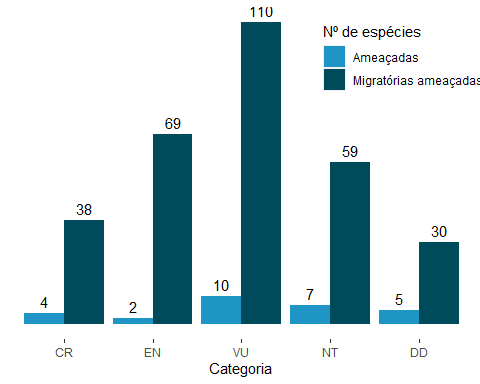
\includegraphics[width=0.65\linewidth]{04-cap03_files/figure-latex/09-1} 

}

\caption{Número total de espécies ou subespécies de aves residentes ameaçadas (cor clara) e de espécies ou subspécies migratórias ameaçadas (cor escura), por categoria: Criticamente em Perigo (CR), Em Perigo (EN) e Vulnerável (VU), de acordo com a Portaria nº 444/2014 (MMA 2014) e Quase Ameaçada (NT) e com Dados Insuficientes (DD), de acordo com o Livro Vermelho (ICMBio 2018).}\label{fig:09}
\end{figure}

Das 16 espécies de aves consideradas migratórias e categorizadas em algum grau de ameaça (CR, EN e VU), nove possuem como vetores de ameaça as atividades associadas à agropecuária, oito sofrem com os diversos impactos causados por distúrbios humanos em áreas de turismo e recreação e por espécies invasoras e/ou oportunistas, sete são alvo de caça e captura (Figura \ref{fig:10}). Além destas ameaças e de tantos outros impactos (Figura 3.2), os parques eólicos têm potencializado ainda mais a pressão sobre as espécies migratórias ameaçadas, motivo para o qual se torna fundamental a realização de estudos robustos, como o Estudo de Impacto Ambiental e Relatório de Impacto Ambiental (EIA/RIMA), em suas respectivas áreas de ocorrência, para que medidas de proteção ou mitigação dos impactos sejam implementadas.

\begin{figure}[H]

{\centering 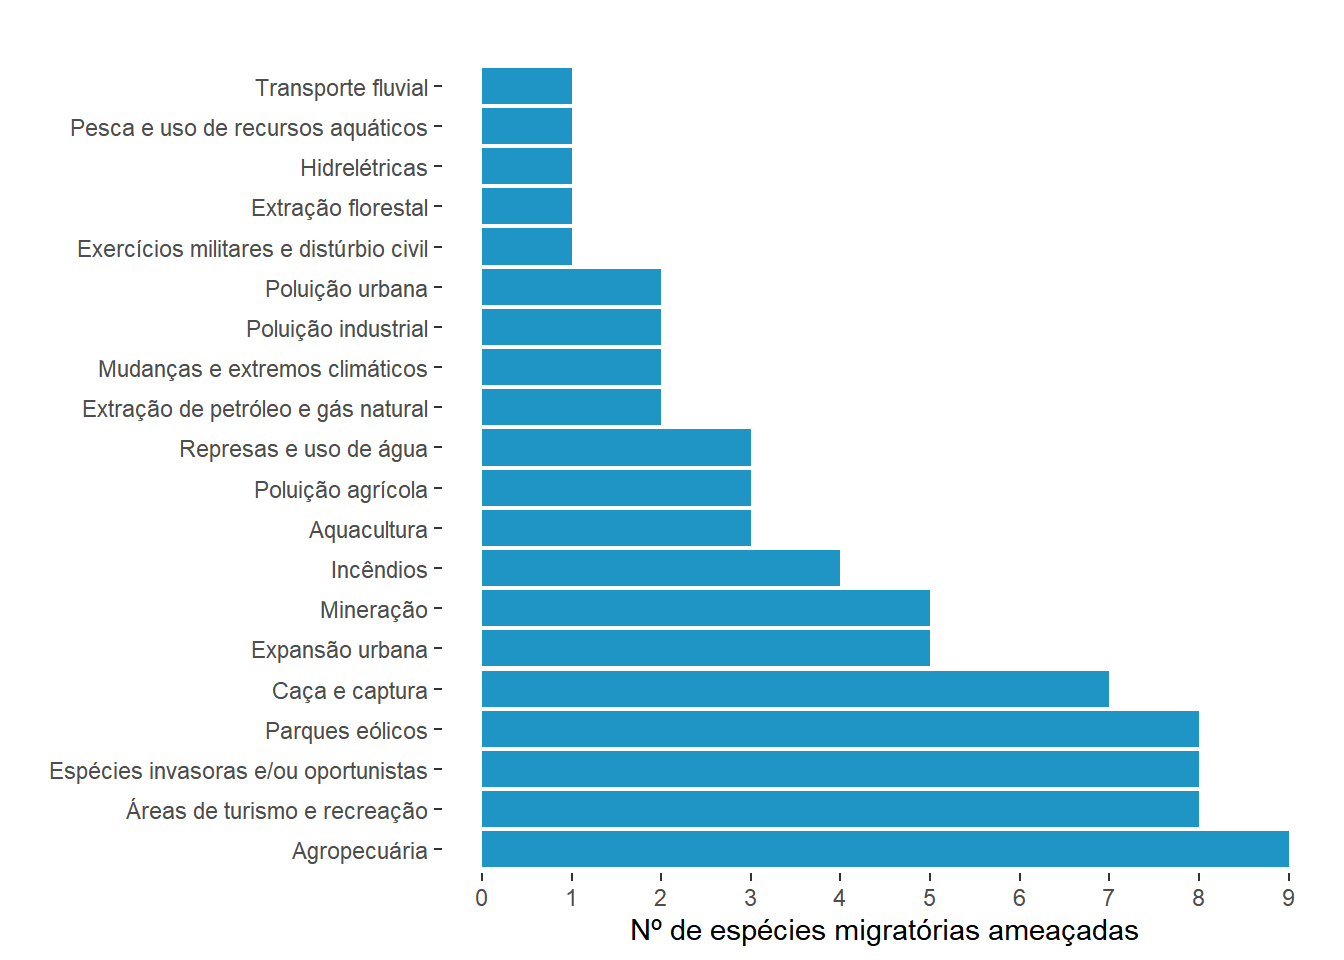
\includegraphics[width=0.85\linewidth]{04-cap03_files/figure-latex/10-1} 

}

\caption{Principais vetores de ameaças às espécies migratórias ameaçadas no Brasil.}\label{fig:10}
\end{figure}

\newpage

\hypertarget{mapa-de-registros-de-aves-ameauxe7adas-de-extinuxe7uxe3o}{%
\section{Mapa de registros de aves ameaçadas de extinção}\label{mapa-de-registros-de-aves-ameauxe7adas-de-extinuxe7uxe3o}}

O Brasil abriga uma das maiores riquezas do mundo em aves, com 1.971 espécies (Pacheco et al.~2021). Infelizmente, cerca de 12\% dessa avifauna encontra-se ameaçada de extinção. Conciliar as intervenções humanas e a conservação das aves nos diferentes ecossistemas naturais brasileiros é uma missão desafiadora.

A Resolução CONAMA nº 462/2014 traz, em seu artigo 3, parágrafo 3, inciso VII, a exigência de EIA/RIMA e audiências públicas para empreendimentos que estejam localizados em áreas de ocorrência de espécies ameaçadas de extinção, conforme listas oficiais. A fim de apoiar os órgãos licenciadores, o CEMAVE elaborou um mapa (Figura \ref{fig:11}) indicando as áreas onde há registros das espécies de aves ameaçadas que constam da lista oficial vigente (Portaria MMA nº 444/2014), com base nos bancos de dados utilizados por este Centro. Esses dados não esgotam todos os registros de aves ameaçadas no Brasil, mas indicam áreas onde sabidamente elas foram registradas e que, portanto, devem ser consideradas no momento de se definir o grau de impacto do empreendimento.

Para a elaboração do mapa que indica as áreas com ocorrência de aves ameaçadas foi utilizada uma grade com células quadradas de 10' (minutos\footnote{Unidade de medida do Sistema de Coordenadas Geográficas: graus, minutos e segundos.}) (aproximadamente 18 km) de lado, que foi criada e sobreposta ao território brasileiro, incluindo as ilhas oceânicas. Todos os registros de ocorrência de aves ameaçadas dos bancos de dados utilizados pelo CEMAVE foram sobrepostos a essa grade de células. Todas as células que continham esses registros foram marcadas e indicam no mapa as áreas de ocorrência de aves ameaçadas no Brasil. Um arquivo do tipo \emph{shapefile} com esta grade pode ser obtido via \emph{download} no \href{https://www.icmbio.gov.br/portal/}{Portal do ICMBio} para se poder localizar com precisão as áreas indicadas no mapa. É importante destacar que a grade de células utilizada é a mesma dos métodos que determinaram as Áreas de Concentração de Aves Migratórias (ver capítulo 7), de modo a padronizar a metodologia e delimitar com precisão a localização geográfica das áreas elencadas no presente relatório.

Os dados de ocorrência de espécies de aves utilizados foram obtidos no \href{http://ara.cemave.gov.br}{Atlas de Registros de Aves Brasileiras - ARA} e no Sistema de Avaliação da Biodiversidade (SALVE), sob responsabilidade do CEMAVE, bem como no sítio eletrônico \href{http://www.wikiaves.com}{``WikiAves - Enciclopédia das Aves do Brasil''}. Esses dados são uma combinação de registros compilados de publicações científicas e dados fornecidos por pesquisadores, colaboradores e observadores de aves, por meio da ciência cidadã. A lista de espécies seguiu a nomenclatura proposta pelo Comitê Brasileiro de Registros Ornitológicos - CBRO (Pacheco et al.~2021).

\begin{figure}[H]

{\centering \includegraphics[width=0.7\linewidth]{imagens/cap03/Figura_3.3} 

}

\caption{Áreas com registros de aves ameaçadas conforme Portaria MMA nº 444/14.}\label{fig:11}
\end{figure}

\newpage

\hypertarget{referuxeancias-bibliogruxe1ficas-2}{%
\section{Referências bibliográficas}\label{referuxeancias-bibliogruxe1ficas-2}}

IUCN (Standards and Petitions Committee). 2022. Guidelines for Using the IUCN Red List Categories and Criteria. Version 15. Prepared by the Standards and Petitions Committee. Disponível em: \url{https://www.iucnredlist.org/resources/redlistguidelines} Acesso em: {[}22/02/2022{]}.

ICMBio (Instituto Chico Mendes de Conservação da Biodiversidade). 2018. Livro Vermelho da Fauna Brasileira Ameaçada de Extinção: Volume I. 1ª. ed.~Brasília, DF: ICMBio/MMA. 492p. Disponível em: \url{https://www.icmbio.gov.br/portal/images/stories/comunicacao/publicacoes/publicacoes-diversas/livro_vermelho_2018_vol1.pdf} Acesso em: {[}22/02/2022{]}.

MMA (Ministério do Meio Ambiente). 2014. Portaria MMA 444/2014. Lista da Fauna Ameaçada Vertebrados e Invertebrados Terrestres. p.121-125.

Mittermeier, R.A., Robles, G.P., Mittermeier, C.G. 1997. Megadiversity: Earth's biologically wealthiest nations. 501p.

Pacheco, J.F., Silveira, L.F. Aleixo, A., Agne, C.E., Bencke, G.A., Bravo, G.A. et al.~2021. Annotated checklist of the birds of Brazil by the Brazilian Ornithological Records Committee --- second edition. Ornithology Research 29: 94--105. \url{http://doi.org/10.1007/s43388-021-00058-x}

\hypertarget{cap4}{%
\chapter{Por que as aves são sensíveis aos empreendimentos eólicos?}\label{cap4}}

\pagestyle{headings}

\textbf{Manuella Andrade de Souza\textsuperscript{1}, Patrícia Pereira Serafini\textsuperscript{2}, Érika Machado Costa Lima\textsuperscript{1} \& Andrei Langeloh Roos\textsuperscript{2}}

\emph{1. Centro Nacional de Pesquisa e Conservação de Aves Silvestres -- CEMAVE}\\
\emph{Instituto Chico Mendes de Conservação da Biodiversidade -- ICMBio}\\
\emph{Floresta Nacional da Restinga de Cabedelo}\\
\emph{BR-230 Km 10}\\
\emph{58108-012, Cabedelo, PB}

\emph{2. Centro Nacional de Pesquisa e Conservação de Aves Silvestres -- CEMAVE}\\
\emph{Instituto Chico Mendes de Conservação da Biodiversidade -- ICMBio}\\
\emph{Estação Ecológica Carijós}\\
\emph{Rodovia Maurício Sirotski Sobrinho s/n - Trevo Jurerê}\\
\emph{88053-700 Florianópolis, SC}

O setor de energia elétrica demanda grandes obras de infraestrutura que produzem mudanças significativas no ambiente natural. Essas condições alteradas geram conflitos decorrentes dos impactos sobre a biodiversidade e o ambiente socioeconômico. Portanto, é necessário assegurar que este desenvolvimento gere o menor impacto negativo possível. Como signatário da Convenção sobre a Conservação das Espécies Migratórias de Animais Silvestres (CMS, do inglês \emph{Convention on Migratory Species}), o Brasil tem o compromisso de envidar esforços para conciliar a exploração do potencial eólico e a conservação das espécies migratórias de interesse global (Resolução nº 7.5 da CMS).

Impactos da instalação dos parques eólicos \emph{onshore}, como a perda de \emph{habitat} por supressão vegetal decorrente da abertura de vias de acesso, e intensificação do tráfego, são sentidos por todos os grupos animais. A biota terrestre voadora (aves, morcegos e insetos) é a mais vulnerável à geração de energia por parques eólicos, principalmente pelos impactos da instalação de aerogeradores, redes de transmissão e de distribuição (Saidur et al.~2011, Schuster et al.~2015, Voigt 2021).

Com relação às aves, a extensão do impacto varia conforme a espécie, a estação, a localização e a disposição ou configuração dos empreendimentos. A localização é tão importante que um parque eólico grande, mas cuidadosamente localizado, pode ter um menor impacto do que um parque eólico menor, mas localizado incorretamente (Gode 2020). Os impactos podem ser permanentes ou temporários, levando em consideração que todo empreendimento possui pelo menos três fases: a implantação, a operação e o descomissionamento, com impactos característicos de cada fase (Figura \ref{fig:12}).

\begin{figure}[H]

{\centering 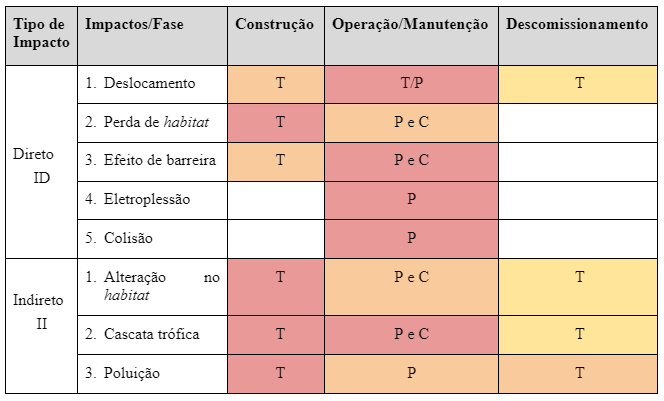
\includegraphics[width=0.75\linewidth]{imagens/cap04/Figura_4.1} 

}

\caption{Principais impactos, diretos e indiretos, identificados em cada fase do empreendimento . Cores e letras são uma proposta de representar a intensidade, temporalidade e efeito do impacto em cada fase: vermelho - maior intensidade, laranja - intensidade média e amarelo - menor intensidade. T - temporário P  -  permanente; C - de caráter cumulativo. Adaptado de: Gode (2020)}\label{fig:12}
\end{figure}

Este capítulo busca responder porque as aves são sensíveis aos empreendimentos eólicos, reunindo informações básicas e mais recentes de publicações técnico-científicas sobre os impactos negativos de empreendimentos eólicos terrestres (\emph{onshore}) sobre a avifauna.

\hypertarget{impactos-ambientais-da-implantauxe7uxe3o-e-operauxe7uxe3o-de-parques-euxf3licos}{%
\section{Impactos ambientais da implantação e operação de parques eólicos}\label{impactos-ambientais-da-implantauxe7uxe3o-e-operauxe7uxe3o-de-parques-euxf3licos}}

Embora já existam milhares de empreendimentos eólicos \emph{onshore} pelo globo, as informações publicadas sobre os impactos desses empreendimentos baseiam-se, principalmente, em parques eólicos localizados na Europa, América do Norte e África do Sul (Agudelo et al.~2021, Marques et al.~2014, Masden et al.~2009, Perold et al.~2020, Schuster et al.~2015, Wang et al.~2015). Os impactos ambientais associados ainda não são totalmente compreendidos para a biodiversidade tropical e o monitoramento dos impactos de empreendimentos eólicos na América Latina é também escasso (Agudelo et al.~2021). Como agravante, os poucos estudos de monitoramento dos impactos nem sempre são desenhados adequadamente (e.g., por não considerarem a taxa de remoção de indivíduos feridos ou mortos por colisão), e as taxas de mortalidade nos parques eólicos, mesmo reduzidas, podem incrementar consideravelmente o risco de extinção de espécies longevas com populações pequenas (Carrete et al.~2009). Os impactos dos parques eólicos podem ser classificados em três tipos: impactos diretos, indiretos e cumulativos (Bennun et al.~2021, Gode 2020).

Os \textbf{impactos diretos} (ID) podem ser divididos em cinco categorias: deslocamento; perda de \emph{habitat}; efeito de barreira; eletroplessão e colisão.

\begin{itemize}
\tightlist
\item
  ID 1. Deslocamento: o efeito de deslocamento - ou alienação, conforme EPHC (2010) - ocorre quando indivíduos, grupos ou populações inteiras deixam de utilizar a área de influência direta do empreendimento, buscando áreas alternativas para as suas atividades de forrageio e reprodução. A distância desses deslocamentos depende da espécie e da localização e tamanho dos aerogeradores. Tal efeito é agravado quando áreas alternativas não existem ou já estão ocupadas.
\item
  ID 2. Perda de \emph{habitat}: para implantação de um parque eólico, invariavelmente, é necessária a supressão de vegetação, a abertura de acessos e a terraplanagem para construção de passagens, o que acarreta alterações nas condições naturais e sistêmicas originais, tornando o \emph{habitat} indisponível para certas espécies. Novas atividades ou usos da terra podem surgir após a implantação, gerando nova perda de \emph{habitat} e aumentando o impacto sobre a biodiversidade.
\item
  ID 3. Efeito de barreira: ocorre quando indivíduos ou populações, instintivamente ou por aprendizado, passam a evitar os parques eólicos em suas rotas, sejam elas diárias ou sazonais. Se, por um lado, ficam menos sujeitos a colisões, por outro podem, em certa escala, estar comprometendo parte de sua locação energética, com desconhecidos efeitos sobre a sobrevivência e/ou sucesso reprodutivo dos indivíduos em longo prazo (Hötker et al.~2006). As espécies que migram em grandes bandos em determinadas rotas são particularmente afetadas. Obstáculos nos trechos utilizados por espécies migratórias não apenas causam fatalidades, mas podem exigir um gasto energético extra para os indivíduos evitarem os obstáculos ou mesmo provocar o abandono de pontos de parada cruciais para o seu descanso e reposição alimentar. A importância do efeito de barreira tem sido monitorada com aves marcadas, sendo bastante sensível ao efeito cumulativo e de amostragem, e tem aumentado conforme se aumenta o número de empreendimentos construídos, sejam contíguos ou não.
\item
  ID 4. Eletroplessão: a eletroplessão ocorre por choque elétrico em linhas de distribuição do parque eólico. Esse impacto é pouco significativo nos postes das linhas de transmissão de alta tensão, mas em postes de linhas de baixa ou média tensão pode ser importante e afetar desproporcionalmente algumas espécies que usam estes postes durante atividades diárias, como descanso, poleiros de caça ou para nidificação.
\item
  ID 5. Colisão: a colisão ocorre quando os animais voadores não conseguem se esquivar das estruturas dos parques eólicos, em especial das pás dos aerogeradores em movimento, linhas de coleta entre torres e linhas de transmissão. As aves que voam na área varrida pelas pás do aerogerador estão sob maior risco de colisão e menor chance de desvio, com potencial para sofrerem injúria grave ou fatal. Este risco se aplica tanto para as espécies residentes como para as migratórias. Dentre todos os impactos, a colisão é o mais facilmente identificável. Contudo, sua mensuração, em geral, é falha devido, dentre outros fatores, ao pequeno esforço comumente destinado ao monitoramento e à intensa remoção de carcaças por predadores ou espécies necrófagas. Instalações de energia eólica mal localizadas podem ter índices de fatalidade consideravelmente elevados.
\end{itemize}

Os \textbf{impactos indiretos} (II) podem ser divididos em três categorias: alteração no \emph{habitat}, cascata trófica e poluição.

\begin{itemize}
\tightlist
\item
  II 1. Alteração no \emph{habitat}: após as perdas diretas com a implantação de um parque eólico, alterações no \emph{habitat} original podem ocorrer em razão das interferências das novas estruturas, acessos modificados e mesmo aumento do acesso às áreas. Processos erosivos gerados pela mudança e/ou interferência nos padrões de vento causados pelas aerogeradores, supressão de vegetação, abertura de acessos e a terraplanagem para construção de passagens são fatores que geram as alterações, podendo causar perda do \emph{habitat} para determinadas espécies. Podemos citar, especificamente, alguns desdobramentos deste tipo de impacto:
\item
  II 1.1. Perturbações: ocorre quando uma espécie persiste na área mesmo após a instalação do empreendimento, mas há prejuízos à sobrevivência e/ou ao sucesso reprodutivo dos indivíduos, ameaçando a permanência das populações em médio e longo prazos. O efeito do estresse sobre a sobrevivência e o sucesso reprodutivo de animais silvestres é bem documentado. Contudo, no contexto de empreendimentos eólicos, não há estudos que tratam da magnitude deste impacto.
\item
  II 1.2. Aumento de caça: a ocupação da área do empreendimento pode introduzir nova atividade/uso da terra, gerando impacto sobre a biodiversidade. A abertura de estradas para a implantação do empreendimento pode facilitar a entrada de pessoas na região e gerar um aumento na pressão de caça sobre as espécies da área.
\item
  II 1.3. Introdução de espécies exóticas invasoras: a movimentação de equipamentos, pessoas e materiais provenientes de outras áreas pode facilitar a introdução de espécies exóticas na área. Além disso, a criação de novos \emph{habitat} ou espaços abertos pode facilitar a expansão das espécies exóticas.
\item
  II 2. Cascata trófica: impacto ainda pouco conhecido, mas há evidências sobre alterações na disponibilidade de presas na região dos parques eólicos. Tais mudanças nos padrões de abundância de espécies afetam a dinâmica predador-presa e, com isso, causam um efeito cascata e alterações nas funções do ecossistema. Estudos em longo prazo bem conduzidos ajudariam a elucidar essa questão.
\item
  II 3. Poluição: embora os exemplos de impactos de poluição relacionados a empreendimentos eólicos sejam limitados, eles foram amplamente demonstrados para outros tipos de desenvolvimento de infraestrutura. Como tipos de poluição podemos elencar: poeira, resíduos sólidos/líquidos, iluminação e barulho/vibração. Dentre estes podemos destacar, pela maior importância:
\item
  II 3.1. Poluição luminosa: sob certas circunstâncias, a sinalização luminosa pode confundir e mesmo atrair as aves, especialmente sob mau tempo. De qualquer forma, luzes artificiais costumam atrair insetos e, por consequência, aves e morcegos em busca de alimentos.
\item
  II 3.2. Poluição sonora: trata-se da perturbação crônica gerada a partir das vibrações dos componentes mecânicos do aerogerador e pela aerodinâmica da estrutura quando em operação. O ruído de instalação, de caráter agudo, é mais diversificado, contemplando o maquinário, o trânsito, entre outros. Há um documento disponível voltado exclusivamente para as diretrizes de mitigação de ruídos em parques eólicos, produzido pela agência de proteção ambiental da Austrália (EPA 2009).
\end{itemize}

Os \textbf{impactos cumulativos} são o resultado dos impactos de desenvolvimento do projeto, somados com os efeitos sucessivos e/ou combinados resultantes das atividades humanas existentes, planejadas e/ou esperadas no futuro (Bennun et al.~2021). Podem surgir da sequência de múltiplos projetos similares (e.g., parques eólicos) ou devido à soma de impactos (agregada ou potencializada) de diferentes fontes (e.g., parques eólicos, estradas, desmatamento). Quando comparados aos demais impactos, são menos conhecidos. Em nível populacional, supõe-se que as espécies de aves migratórias e aquelas que percorrem grandes áreas para se alimentar podem sofrer mortalidade cumulativa significativa, pois uma proporção maior da população pode encontrar múltiplos aerogeradores durante seus movimentos.

\hypertarget{fatores-que-afetam-o-risco-de-colisuxe3o}{%
\section{Fatores que afetam o risco de colisão}\label{fatores-que-afetam-o-risco-de-colisuxe3o}}

Centenas de espécies são suscetíveis a colisões e, tradicionalmente, rapinantes, aves marinhas e outras aves de médio e grande porte têm sido reportadas como os principais grupos afetados por aerogeradores. No entanto, estes grupos são detectados mais facilmente pelos pesquisadores e têm uma taxa de remoção por carniceiros menor, o que pode levar a um viés nos resultados encontrados, a depender do desenho amostral e do método de registro utilizado. Isto fica claro em alguns estudos que apontam os Passeriformes como o grupo que responde pela maior parte dos casos de colisão, chegando a 82\% dos registros (Erickson et al.~2001).

Contudo, a gravidade do impacto das colisões está relacionada a outros fatores. Ordens com predomínio de aves de médio e grande porte, quando comparadas com Passeriformes, de um modo geral, apresentam populações menores, maior proporção de espécies ameaçadas de extinção e resposta mais lenta a aumentos na taxa de mortalidade (Hötker et al.~2006).

Conforme a literatura disponível, a mortalidade detectada nos parques eólicos é muito variável e parece depender também do contexto local. Mesmo parques próximos podem apresentar taxas de colisão bastante discrepantes, com diferenças significativas para um mesmo táxon. Estudos indicam taxas totais observadas que variaram de zero a 64 mortes por aerogerador por ano (Lekuona 2001 in Atienza et al.~2011).

Algumas espécies têm maiores chances de colisão (Drewitt \& Langston 2008), mas diversos fatores parecem interferir nas taxas de colisão, podendo ser ambientais, paisagísticos, além daqueles relacionados às características biológicas das espécies (Thaxter et al.~2017). A seguir, descrevemos alguns destes fatores.

\emph{Tempo e clima}

Nesses fatores, o componente de maior destaque são as tempestades, que agravam o risco de colisão devido à maior velocidade do vento e à baixa visibilidade, decorrente das chuvas, nuvens ou neblina. Ao contrário das aves, os morcegos parecem colidir menos em períodos de fortes ventos, talvez simplesmente por evitarem o voo em condições extremas. As colisões tendem a ser mais frequentes durante a noite, com maior risco sob céu nublado ou com ocorrência de neblina.

\emph{Iluminação}

O impacto do uso de luzes sinalizadoras ainda necessita de pesquisa, principalmente no hemisfério austral, contudo estudos mostram que as cores destas luzes e sua intermitência interferem nas taxas de colisão, além da altura da disposição da iluminação (Rebke et al.~2019). O \emph{U.S. Fish and Wildlife Service} (USFWS 2003) aponta que as luzes brancas atraem mais as aves que as vermelhas, fazendo-as voar em seu entorno. Gehring et al.~(2009) não encontraram diferenças significativas quanto às cores, mas observaram que a sinalização intermitente (luzes do tipo \emph{flashing} ou \emph{strobe}) reduziu a atração de aves quando comparada a luzes contínuas. Luzes de cor verde, vermelha ou azul têm sido reportadas como menos atrativas para aves (Evans et al.~2007, Poot et al.~2008, Rebke et al.~2019). Sendo a iluminação necessária, essa deve ser restrita ao mínimo, ser intermitente e preferencialmente de cor vermelha (Rebke et al.~2019, Kerlinger et al.~2010).

\emph{Características geográficas}

Alguns acidentes geográficos como penínsulas e estreitos podem representar área de maior risco de colisão, visto que normalmente compõem rotas de aves migratórias. O Estreito de Gibraltar, entre Europa e África, é tradicionalmente citado como um sítio crítico para colisões de aves com aerogeradores, por reunir estas duas situações paisagísticas: ser um estreito entre duas grandes penínsulas (De Lucas et al.~2004, Drewitt \& Langston 2008). Relevo acidentado como cristas, vales e vertentes, que causam turbulência nas correntes de ar ou geram correntes ascendentes, tendem a ocasionar maior número de colisões.

\emph{Disposição e altura dos aerogeradores}

A disposição dos aerogeradores na paisagem pode afetar sobremaneira o risco de colisão. A distribuição linear das torres, perpendicular à principal direção dos ventos, é o modelo menos indicado. O impacto pode ser ainda maior se os aerogeradores estiverem alinhados paralelamente a vales ou a serras utilizadas como referência para as aves em rota de voo (Figura \ref{fig:13}). Parques em áreas planas, com aerogeradores agrupados em blocos e com largos corredores de passagem entre eles, tendem a ter taxas de colisão menores por aparelho. Aerogeradores isolados tendem a possuir uma taxa de colisão maior.

Outro fator que pode influenciar a taxa de colisão é a altura dos aerogeradores (e.g., aerogeradores maiores têm maior probabilidade de interceptar o voo de aves que migram à noite). Para a próxima década, são esperados aerogeradores com altura total superior a 300 m. Todavia, aerogeradores maiores, com maior capacidade, poderiam implicar menor número de aerogeradores por parque eólico, sem que a produção de energia seja comprometida (De Lucas et al.~2004, Drewitt \& Langston 2008).

\begin{figure}[H]

{\centering 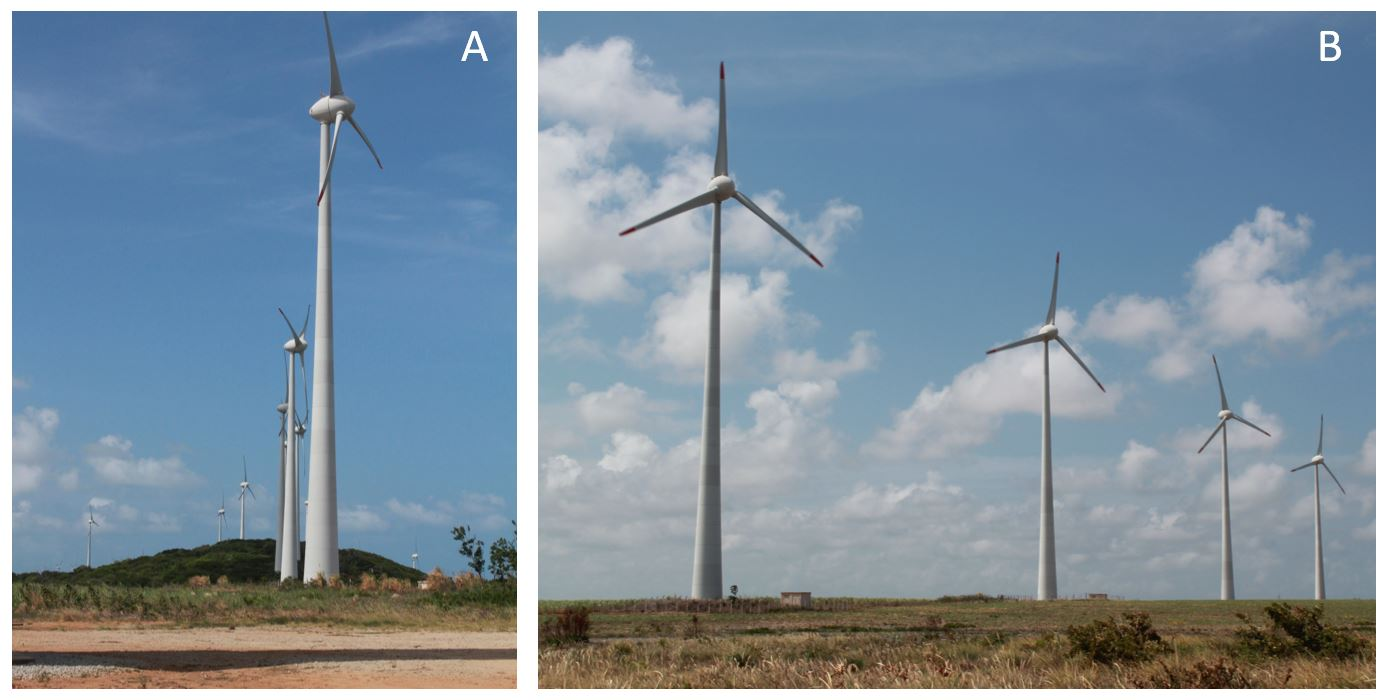
\includegraphics[width=0.75\linewidth]{imagens/cap04/Figura_4.2ab} 

}

\caption{Exemplos de alinhamentos de aerogeradores, Parque Eólico na Paraíba. Foto: Andrei L. Roos}\label{fig:13}
\end{figure}

\emph{Densidade de fauna}

É esperada que a abundância (densidade) de aves também seja positivamente correlacionada às taxas de colisão. A densidade de aves pode aumentar se as estruturas do parque eólico atraírem insetos, roedores e outras espécies utilizadas como presas pelas aves (Drewitt \& Langston 2008).

\emph{Morfologia das aves}

O campo de visão e a acuidade visual das aves é muito variável. A maioria delas apresenta visão lateral (Martin 2011) com um ``ponto cego'' frontal, ao passo que as aves de rapina possuem uma boa visão binocular, mas sua visão periférica é limitada, tendo, portanto, uma grande zona cega (Bevanger 1998, Drewitt \& Langston 2008). As restrições geradas pelo tipo de visão de cada espécie podem interferir no risco de colisão. Como regra geral, aves com visão lateral, aves com grande área cega acima e atrás da cabeça e aves sem fóvea (como Galliformes) têm maior risco de colisão, pois têm dificuldade de ver objetos à frente (Bernardino et al.~2018). Além disso, as restrições mecânicas impostas pelo tamanho, proporção e forma da asa (Wang \& Clarke 2015) geram baixo poder de manobrabilidade, aumentando o risco de colisão para algumas espécies.

\emph{Comportamento das aves}

Certas características comportamentais tornam algumas aves particularmente sujeitas à colisão: a formação de grandes bandos para deslocamento ou migração (Larsen \& Clausen 2002), o hábito de planar e utilizar correntes termais, o voo noturno e crepuscular (Drewitt \& Langston 2008), voos nupciais ou para atividades predatórias (Orloff \& Flannery 1992, Madders \& Whitfield 2006) ou, ainda, para defesa territorial (Langston \& Pullan 2003). A fase de vida da ave também pode interferir no risco de colisão: pais com filhotes para alimentar (Langston \& Pullan 2003) precisam de itinerários mais curtos e arriscam-se mais (Drewitt \& Langston 2008); jovens são menos experientes e ágeis que os adultos, havendo maior risco de colisão para esse grupo etário (Drewitt \& Langston 2008).

A altura de voo de cada espécie também interfere no risco de colisão. Registros de radar na costa da Inglaterra revelaram que Passeriformes migram durante o dia abaixo de 1.500 m e à noite podem subir a 4.000 m (Sick 1985). Espécies migratórias de longas distâncias em voos diretos (non-stop) atingem altitudes em torno de 6.000 m, com variações da altitude entre dia e noite, atingindo as maiores altitudes à noite (Pough et al.~1993, Senner et al.~2018, Lindström et al.~2021). Embora Sick (1985) afirme que geralmente as migrações são realizadas abaixo de 600 m, variando conforme as condições meteorológicas, pouco se sabe sobre as altitudes de migrações na América Latina e mais estudos são necessários para responder essa questão. Mesmo as espécies que realizam voos em altitudes elevadas são sujeitas a colisões nos momentos de aterrissagem e decolagem, ou em condições de mau tempo quando voam a altitudes menores, a depender das suas taxas de ascensão vertical e comportamento de voo, ou ainda em voos de deslocamentos diários (Piersma et al.~1997, Bernardino et al.~2018, Larsen \& Clausen 2002).

Segundo Orloff \& Flannery (1992) a velocidade de voo também afeta a capacidade da ave em detectar o obstáculo, assim como seu tempo de reação. As aves de rapina de voo mais rápido (como os falconídeos) são mais vulneráveis à colisão e eletroplessão que os demais rapinantes. Espécies que apresentam comportamento de peneirar (planar) contra o vento, examinando o solo atentamente, a alturas de cerca de 30 m antes de descer sobre a presa, também podem ser vulneráveis a colisões. As fragatas, por exemplo, se destacam devido ao seu hábito de planar. Registros de mortalidade da espécie decorrente de interação com aerogeradores no Brasil foram descritos inclusive para o arquipélago de Fernando de Noronha, onde um único aerogerador foi instalado (P. Serafini, com. pess. 2009).

\hypertarget{principais-grupos-em-risco-e-suas-caracteruxedsticas}{%
\section{Principais grupos em risco e suas características}\label{principais-grupos-em-risco-e-suas-caracteruxedsticas}}

Considerando aspectos peculiares e intrínsecos de diferentes espécies, famílias e ordens da Classe Aves, e com base em estudos específicos que avaliaram os impactos de empreendimentos eólicos sobre esses animais, elencamos, a seguir, alguns grupamentos que compartilham características morfológicas, fisiológicas, ecológicas ou comportamentais que os tornam mais vulneráveis e sensíveis aos impactos relacionados às estruturas de geração e transmissão de energia eólica.

\emph{Passeriformes}

Segundo AWWI (2020) e Erickson et al.~(2001) algumas espécies de Passeriformes podem ser desproporcionalmente afetadas por impactos de parques eólicos devido à sua abundância, biologia ou comportamento. Os impactos sobre essas espécies raramente são considerados significativos ao nível populacional por possuírem, na maioria dos casos, populações relativamente grandes e tempo de geração curto. Contudo, especial atenção deve ser dada a espécies endêmicas ou com área de distribuição restrita, ameaçadas de extinção ou com populações em declínio.

Garcia et al.~(2015) observaram que a fase de construção e instalação dos empreendimentos eólicos potencialmente impõe os efeitos mais severos sobre Passeriformes residentes. Contudo, muitas populações se recuperaram ao longo dos anos após a construção e podem voltar a crescer durante os anos de operação. Por outro lado, presume-se que o ruído relacionado aos aerogeradores e à infraestrutura associada à produção de energia eólica afeta o uso do \emph{habitat}, o comportamento territorial e o sucesso reprodutivo da fauna residente. A qualidade do \emph{habitat} para os Passeriformes florestais parece ser afetada negativamente também pelo ruído antrópico e sua densidade em áreas próximas a instalações geradoras de ruído é menor do que em áreas próximas a instalações onde a produção de energia é mais silenciosa (Bayne et al.~2008).

\emph{Grandes aves planadoras}

As espécies mais suscetíveis ao risco de colisão com aerogeradores e linhas de transmissão são, geralmente, aves de grande porte e que dependem de correntes de ar para a realização de voos planados de longa distância (Figura \ref{fig:14}). Estas espécies podem não possuir a habilidade ou agilidade suficientes para mudar as trajetórias de voo rapidamente frente a um obstáculo inesperado e possuem, em geral, visão restrita a um campo frontal, o que significa que podem não detectar as pás dos aerogeradores (Martin \& Shaw 2010, Marques et al.~2014).

O impacto dos parques eólicos neste grupo de aves pode estar diretamente relacionado à perda de diversos indivíduos de uma mesma população devido à mortalidade por colisão com aerogeradores. Exemplos de grupos com espécies em maior risco de colisão incluem representantes das ordens Accipitriformes e Ciconiiformes (Marques et al.~2014, Thaxter et al.~2017). Além disso, essas aves normalmente têm tempos de geração longos e populações relativamente pequenas, quando comparadas aos Passeriformes, o que aumenta o potencial de efeitos populacionais importantes no somatório da mortalidade de indivíduos pelo impacto com aerogeradores.

Além dos efeitos negativos das colisões, esse grupo é afetado pela perda de \emph{habitat} funcional. Através do comportamento de evitação das áreas de empreendimentos eólicos, essas aves perdem áreas adequadas ao voo planado e forrageio sofrendo com o efeito barreira, perda de \emph{habitat} e deslocamentos, de forma cumulativa (Marques et al.~2020).

\begin{figure}[H]

{\centering 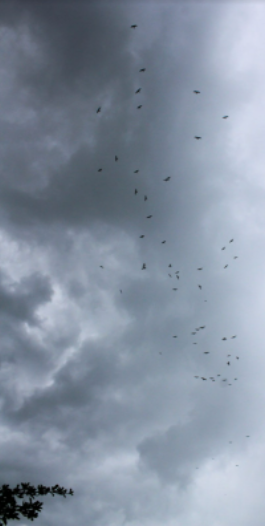
\includegraphics[width=0.4\linewidth]{imagens/cap04/Figura_4.3} 

}

\caption{Bando de gavião-tesoura (\emph{Elanoides forficatus}) em movimento de ascensão vertical durante deslocamento migratório. Foto: Andrei L Roos}\label{fig:14}
\end{figure}



\emph{Aves migratórias}

Alguns estudos apontam que espécies migratórias seriam mais suscetíveis do que espécies residentes, visto estarem expostas ao efeito cumulativo de transitar por vários parques eólicos ao longo de suas rotas, por serem menos familiarizadas com as localidades pelas quais transitam e, muitas vezes, por migrarem em grandes grupos (Hüppop et al.~2019). Dentre as aves migratórias, a ordem Charadriiformes, que compreende as aves limícolas, parece ser a mais vulnerável (Thaxter et al.~2017). Por outro lado, há estudos que indicam que as aves residentes estão diariamente sujeitas à colisão, sendo, portanto, mais suscetíveis (Drewitt \& Langston 2008). Marques et al.~(2014) ressaltam que, a depender do local de instalação, a mortalidade em um parque eólico é frequentemente mais alta para as espécies residentes, à medida que empreendem um número maior de voos na área onde há risco de colisão.

O efeito ``barreira'' gerado pelas estruturas dos aerogeradores possui impactos negativos importantes em rotas de migração (De Lucas et al.~2004). Além disso, a alteração de ambientes naturais para a instalação dos empreendimentos, associada à perda definitiva de \emph{habitat} em pontos de parada ou agregação importantes ao longo de rotas de migração podem representar redução de taxas de sobrevivência e sucesso reprodutivo, ao impor significativo gasto energético para indivíduos migrantes na busca de ambientes que propiciem recursos suficientes para a continuidade de seus ciclos biológicos (Marques et al.~2020).

\emph{Anseriformes, em especial Anatidae}

Estudos de mortalidade direta de Anatidae (i.e., patos e marrecas) causada por sua interação com estruturas relacionadas à energia eólica demonstraram que o risco de colisão é menor para esse grupo, devido ao comportamento e habilidade de evitar as estruturas e aerogeradores (Masden et al.~2009, Wang et al.~2015). No entanto, entende-se que os parques eólicos possuem efeitos indiretos nessas populações, incluindo alterações no uso dos ambientes, padrões de distribuição e deslocamento, que foram considerados como tendo um impacto maior do que os efeitos diretos (Masden et al.~2009, Zhao et al.~2020). Hötker (2017) chegou a classificar Anatidae como um dos grupos mais gravemente afetados e deslocados e sugeriu que os anatídeos podem abandonar ambientes adequados dentro ou próximos a um parque eólico, ou usá-los com menos frequência do que o fariam na ausência destes empreendimentos.

\emph{Aves de grande porte com comportamento de empoleirar-se e espécies com alta carga alar}

O grupo de espécies em maior risco de eletroplessão em linhas de transmissão, inclusive associadas a empreendimentos eólicos, são aves de rapina e aves de grande porte que possuem comportamento de empoleirar-se. Essas aves costumam usar os postes, que sustentam as linhas de transmissão, como poleiros para descanso ou para permanecerem à espreita e desempenhar seu comportamento de captura de presas na região (predação), além de, muitas vezes, usarem as estruturas instaladas como locais de nidificação ou mesmo descanso (Figura \ref{fig:15}). Sua grande envergadura aumenta o risco de contato com mais de um cabo da linha de transmissão durante o voo ou quando pousadas, criando inadvertidamente um curto-circuito. A eletroplessão pode ocorrer em duas situações: quando a ave toca ao mesmo tempo dois fios ou quando toca um fio energizado e o poste, de forma a fechar o circuito. Quase todas as eletroplessões ocorrem em linhas de baixa e média tensão (\textless{} 15 kV); linhas de alta tensão raramente possuem componentes próximos o suficiente para uma ave tocar ambos cabos ao mesmo tempo. Fatores de risco associados incluem as dimensões das estruturas potencialmente usadas como poleiro, o espaço entre linhas e outras estruturas (Dixon et al.~2018, 2019). Na região do Raso da Catarina, Bahia, mais de 50 casos de mortes por eletroplessão de araras-azuis-de-lear (\emph{Anodorhynchus leari}) já foram registrados e têm sido acompanhados pelo CEMAVE. As araras possuem o comportamento de pousar em estruturas altas e devido sua grande envergadura e comportamento social podem fechar o circuito tocando os diferentes cabos da rede. A espécie é também suscetível à colisão com estruturas (aerogeradores, linhas de distribuição/transmissão).

Outro grupo que pode ser afetado pela mortalidade em contato com linhas de transmissão e infraestrutura relacionadas à produção e distribuição de energia elétrica são as aves com alta carga alar, ou seja, maior proporção entre massa corporal e área da asa, como por exemplo, rapinantes. Estes animais com alta carga alar estão em maior risco de colisão devido à baixa manobrabilidade (De Lucas et al.~2008).

\begin{figure}[H]

{\centering 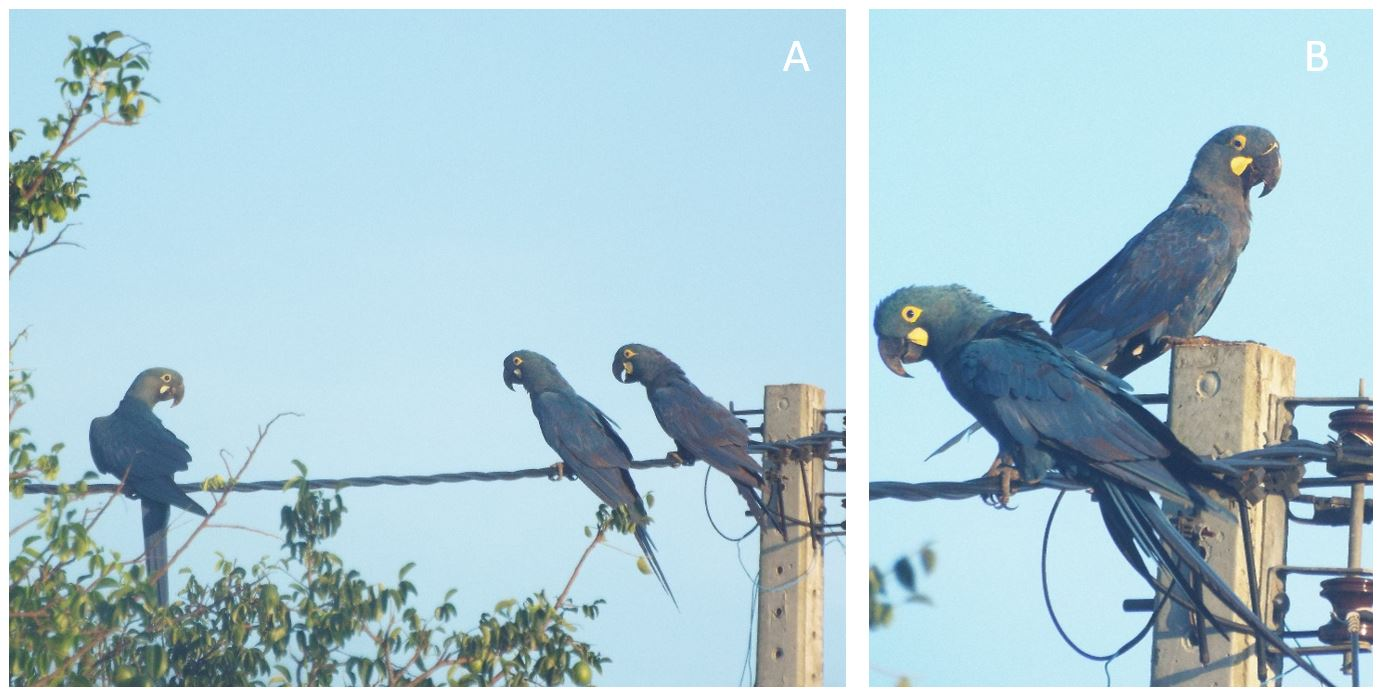
\includegraphics[width=0.75\linewidth]{imagens/cap04/Figura_4.4ab} 

}

\caption{Utilização de estruturas de linhas de transmissão por araras-azuis-de-lear. Fotos: Jaelson Gomes}\label{fig:15}
\end{figure}

\hypertarget{mudanuxe7a-na-composiuxe7uxe3o-e-riqueza-de-aves-em-comunidades-afetadas-por-empreendimentos-euxf3licos}{%
\section{Mudança na composição e riqueza de aves em comunidades afetadas por empreendimentos eólicos}\label{mudanuxe7a-na-composiuxe7uxe3o-e-riqueza-de-aves-em-comunidades-afetadas-por-empreendimentos-euxf3licos}}

A construção de parques eólicos pode afetar a comunidade de aves devido à degradação e perda de \emph{habitat} ou devido à mortalidade direta em função das novas estruturas construídas (Bennun et al.~2021). Em um estudo recente e inédito no Brasil, Falavigna et al.~(2020) analisaram mudanças na composição e riqueza de espécies nas fases de pré-implantação, implantação e operação de um parque eólico do Rio Grande do Sul e observaram uma redução na riqueza de 146 espécies da fase de pré-implantação para 115 durante a implantação e 122 na fase de operação dos parques eólicos. Quanto à composição de espécies, registraram diferenças entre as fases pré-implantação e operação, ao passo que a fase de implantação não difere das fases de pré-implantação e operação. Concluíram que tanto a riqueza quanto a composição da comunidade de aves mudaram após o início da fase de operação, indicando o possível impacto negativo do parque eólico em longo prazo.

Vieira-Filho et al.~(2014) analisaram uma comunidade de aves antes e após a implantação de um complexo eólico no Rio Grande do Norte e observaram redução maior que 20\% na riqueza de espécies, enquanto a abundância total sofreu redução superior a 30\%.

Apesar de existirem resultados apontando que as mudanças antrópicas na área do parque eólico podem influenciar na composição das espécies, estudos de longo prazo são necessários para verificar se o grau desses efeitos negativos pode diminuir ao longo dos anos de operação, pois mesmo que muitas espécies abandonem a área por não serem capazes de se habituar, muitas outras podem se adaptar (Langston \& Pullan 2003, Falavigna et al.~2020).

A maioria dos parques eólicos no Brasil está localizada em áreas ambientalmente sensíveis ou de alta prioridade para a conservação (52\% em áreas de vegetação nativa e 10\% em dunas costeiras), de forma diferente do que ocorre na Europa, onde a maior parte está localizada em terras agrícolas (Neri et al.~2019, Turkovska et al.~2021). Tais diferenças de padrão de ocupação levam a diferenças nos impactos ambientais e de uso do solo. Se tal padrão de ocupação continuar com a expansão do uso da energia eólica, haverá uma tendência de aumentarem os conflitos ambientais decorrentes da instalação, operação e descomissionamento dos empreendimentos. Dada a necessidade de expansão das fontes de energia, apesar da necessidade de redução da emissão de gases do efeito estufa, a energia eólica surge como uma alternativa, mas para conciliá-la com a proteção da biodiversidade e seus serviços ambientais é necessário buscar a implantação de parques eólicos fora de áreas ambientalmente vulneráveis, buscando regiões já alteradas por atividades humanas, de forma a minimizar os impactos e conflitos socioambientais.

\newpage

\hypertarget{referuxeancias-bibliogruxe1ficas-3}{%
\section{Referências bibliográficas}\label{referuxeancias-bibliogruxe1ficas-3}}

Agudelo, M.S., Mabee, T.J., Palmer, R., Anderson, R. 2021. Post-construction bird and bat fatality monitoring studies at wind energy projects in Latin America: A summary and review. Heliyon 7: e07251. \url{https://doi.org/10.1016/j.heliyon.2021.e07251}

AWWI (American Wind Wildlife Institute). 2020. Wind turbine interactions with wildlife and their habitats: A summary of research results and priority questions: American wind wildlife institute.

Atienza, J.C., Martín, I., Infante, O., Valls, J. 2011. Directrices para la evaluación del impacto eólico en aves y murciélagos. SEO/BirdLife. Madrid. 53p. Disponível em: \url{https://www.seo.org/wp-content/uploads/2012/05/MANUAL-MOLINOS-VERSION-31_WEB.pdf} Acesso em: {[}22/03/2022{]}.

Bayne, E.M., Habib, L., Boutin, S. 2008. Impacts of chronic anthropogenic noise from energy-sector activity on abundance of songbirds in the boreal forest. Conservation Biology 22: 1186--1193. \url{https://doi.org/10.1111/j.1523-1739.2008.00973.x}

Bennun, L., van Bochove, J., Ng, C., Fletcher, C., Wilson, D., Phair, N., Carbone, G. 2021. Mitigating biodiversity impacts associated with solar and wind energy development: guidelines for project developers. IUCN/The Biodiversity Consultancy. Gland/Cambridge. \url{https://doi.org/10.2305/IUCN.CH.2021.04.en}

Bernardino, J., Bevanger, K., Barrientos, R., Dwyer, J.F., Marques, A.T., Martins, R.C., Shaw, J.M., Silva, J.P., Moreira, F. 2018. Bird collisions with power lines: State of the art and priority areas for research. Biological Conservation 222: 1--13. \url{https://doi.org/10.1016/J.BIOCON.2018.02.029}

Bevanger, K. 1998. Biological and conservation aspects of bird mortality caused by electricity power lines: a review. Biological Conservation 86: 67--76. \url{https://doi.org/10.1016/S0006-3207(97)00176-6}

Biasotto, L.D., Kindel, A. 2018. Power lines and impacts on biodiversity: A systematic review. Environmental Impact Assessment Review 71: 110-119. \url{https://doi.org/10.1016/j.eiar.2018.04.010}

Carrete, M., Sánchez-Zapata, J.A., Benítez, J.R., Lobón, M., Donázar, J.A. 2009. Large scale risk-assessment of wind-farms on population viability of a globally endangered long-lived raptor. Biological Conservation 142: 2954--2961. \url{https://doi.org/10.1016/J.BIOCON.2009.07.027}

De Lucas, M., Janss, G.F.E., Ferrer, M. 2004. The effects of a wind farm on birds in a migration point: the Strait of Gibraltar. Biodiversity \& Conservation 13: 395--407. \url{https://doi.org/10.1023/B:BIOC.0000006507.22024.93}

De Lucas, M., Janss, G.F.E., Whitfield, D.P., Ferrer, M. 2008. Collision fatality of raptors in wind farms does not depend on raptor abundance. Journal of Applied Ecology 45: 1695--1703. \url{https://doi.org/10.1111/J.1365-2664.2008.01549.X}

Dixon, A., Bold, B., Tsolmonjav, P., Galtbalt, B., Batbayar, N. 2018. Efficacy of a mitigation method to reduce raptor electrocution at an electricity distribution line in Mongolia. Conservation Evidence 15: 50--53. \url{https://www.conservationevidence.com/individual-study/6861}

Drewitt, A.L., Langston, R.H.W. 2008. Collision effects of wind-power generators and other obstacles on birds. Annals of the New York Academy of Sciences 1134: 233--266. \url{https://doi.org/10.1196/annals.1439.015}

EPA (Environment Protection Authority). 2009. Wind farms environmental noise guidelines. Disponível em: \url{https://www.epa.sa.gov.au/files/47788_windfarms.pdf} Acesso em: {[}22/02/2022{]}.

EPCH (The Environment Protection and Heritage Council). 2010. National Wind Farm Development Guidelines. Draft. Disponível em: \url{http://www.nepc.gov.au/system/files/resources/8e446a1a-ab93-5f84-99d0-12d3422d2a23/files/draft-national-wind-farm-development-guidelines-july-2010.pdf} Acesso em: {[}09/03/2022{]}.

Erickson, W.P., Johnson, G.D., Strickland, D.M., Young, Jr., D.P., Sernka, K.J., Good, R.E. 2001. Avian Collisions with Wind Turbines: A Summary of Existing Studies and Comparisons to Other Sources of Avian Collision Mortality in the United States. Oakland. \url{https://doi.org/10.2172/822418}

Erickson, W.P., Wolfe, M.M., Bay, K.J., Johnson, D.H., Gehring, J.L. 2014. A comprehensive analysis of small-passerine fatalities from collision with turbines at wind energy facilities. PLoS ONE 9: e107491. \url{https://doi.org/10.1371/JOURNAL.PONE.0107491}

Evans, W.R., Akashi, Y., Altman, N.S., Manville, A.M. 2007. Response of night-migrating songbirds in cloud to colored and flashing light. Disponível em: \url{https://www.researchgate.net/publication/303170066_Response_of_night-migrating_songbirds_in_cloud_to_colored_and_flashing_light} Acesso em: {[}22/02/2022{]}.

Falavigna, T.J., Pereira, D., Rippel, M.L., Petry, M.V. 2020. Changes in bird species composition after a wind farm installation: A case study in South America. Environmental Impact Assessment Review 83: 106387. \url{https://doi.org/10.1016/J.EIAR.2020.106387}

Garcia, D.A., Canavero, G., Ardenghi, F., Zambon, M. 2015. Analysis of wind farm effects on the surrounding environment: Assessing population trends of breeding passerines. Renewable Energy 80: 190--196. \url{https://doi.org/10.1016/j.renene.2015.02.004}

Gehring, J., Kerlinger, P., Manville, A.M. 2009. Communication towers, lights, and birds: Successful methods of reducing the frequency of avian collisions. Ecological Applications 19: 505--514. \url{https://doi.org/10.1890/07-1708.1}

Gode, P. 2020. How to design future wind farms to best mitigate their disturbance effects on birds? Dissertação de mestrado. Universidade de Strathclyde. Glasgow. \url{https://doi.org/10.13140/RG.2.2.18138.36808}

Hötker, H. 2017. Birds: Displacement, p.~157--190. In: Perrow, M.R. (ed). Wildlife and Wind Farms, Conflicts and Solutions. Volume 1 Onshore: Potential Effects. Pelagic Publishing. Exeter.

Hötker, H., Thomsen, K.-M., Jeromin, H. 2006. Impacts on biodiversity of exploitation of renewable energy sources: the example of birds and bats - facts, gaps in knowledge, demands for further research, and ornithological guidelines for the development of renewable energy exploitation. Bergenhusen. Disponível em: \url{https://tethys.pnnl.gov/sites/default/files/publications/Hotker_et_al_Renewable_Energy_on_Biodiversity.pdf} Acesso em: {[}22/02/2022{]}.

Hüppop, O., Michalik, B., Bach, L., Hill, R., Pelletier, S. 2019. Migratory birds and bats, p.~142--173. In: Perrow, M.R. (ed). Wildlife and Wind Farms, Conflicts and Solutions. Volume 3 Offshore: Potential Effects. Pelagic Publishing. Exeter.

Kerlinger, P., Gehring, J.L., Erickson, W.P., Curry, R., Jain, A., Guarnaccia, J. 2010. Night migrant fatalities and obstruction lighting at wind turbines in North America. The Wilson Journal of Ornithology 122(4): 744-754. \url{http://dx.doi.org/10.1676/06-075.1}

Langston, R.H.W., Pullan, J. 2003. Windfarms and Birds: an analysis of the effects of windfarms on birds, and guidance on environmental assessment criteria and site selection issues, p.~1--58. In: Convention on the Conservation of European Wildlife and Natural Habitats. Disponível em: \url{https://tethys.pnnl.gov/sites/default/files/publications/Langston\%20and\%20Pullan\%202003.pdf} Acesso em: {[}22/02/2022{]}.

Larsen, J. K., Clausen, P. 2002. Potential Wind Park Impacts on Whooper Swans in Winter: The Risk of Collision. Waterbirds: The International Journal of Waterbird Biology 25: 327--330. \url{http://www.jstor.org/stable/1522370}

Lindström, Å., Alerstam, T., Andersson, A., Bäckman, J., Bahlenberg, P., Bom, R., Ekblom, R., Klaassen, R.H.G., Korniluk, M., Sjöberg, S., Weber, J.K.M. 2021. Extreme altitude changes between night and day during marathon flights of great snipes. Current Biology 31: 3433-3439.e3. \url{https://doi.org/10.1016/j.cub.2021.05.047}

Madders, M., Whitfield, D.P. 2006. Upland raptors and the assessment of wind farm impacts. Ibis 148: 43--56. \url{https://doi.org/10.1111/j.1474-919X.2006.00506.x}

Marques, A.T., Batalha, H., Rodrigues, S., Costa, H., Pereira, M.J.R., Fonseca, C., Mascarenhas, M., Bernardino, J. 2014. Understanding bird collisions at wind farms: An updated review on the causes and possible mitigation strategies. Biological Conservation 179: 40--52. \url{https://doi.org/10.1016/j.biocon.2014.08.017}

Marques, A.T., Santos, C.D., Hanssen, F., Muñoz, A.R., Onrubia, A., Wikelski, M., et al.~2020. Wind turbines cause functional habitat loss for migratory soaring birds. Journal of Animal Ecology 89(1): 93-103. \url{https://doi.org/10.1111/1365-2656.12961}

Martin, G.R., Shaw, J.M. 2010. Bird collisions with power lines: Failing to see the way ahead? Biological Conservation 143: 2695--2702. \url{https://doi.org/10.1016/j.biocon.2010.07.014}

Martin, G.R. 2011. Understanding bird collisions with man-made objects: a sensory ecology approach. Ibis 153: 239-254. \url{https://doi.org/10.1111/j.1474-919X.2011.01117.x}

Masden, E.A., Haydon, D.T., Fox, A.D., Furness, R.W., Bullman, R., Desholm, M. 2009. Barriers to movement: impacts of wind farms on migrating birds. ICES Journal of Marine Science 66: 746--753. \url{https://doi.org/10.1093/icesjms/fsp031}

Neri, M., Jameli, D., Bernard, E., Melo, F.P.L. 2019. Green versus green? Adverting potential conflicts between wind power generation and biodiversity conservation in Brazil. Perspectives in Ecology and Conservation 17: 131--135. \url{https://doi.org/10.1016/j.pecon.2019.08.004}

Orloff, S., Flannery, A. 1992. Wind Turbine Effects on Avian Activity, Habitat Use, and Mortality in the Altamont Pass and Solano County Wind Resource Areas, 1989-1991. Disponível em \url{https://tethys.pnnl.gov/publications/wind-turbine-effects-avian-activity-habitat-use-mortality-altamont-pass-solano-county} Acesso em: {[}22/02/2022{]}.

Perold, V., Ralston-Paton, S., Ryan, P. 2020. On a collision course? The large diversity of birds killed by wind turbines in South Africa. Ostrich 91: 228--239. \url{https://doi.org/10.2989/00306525.2020.1770889}

Poot, H., Ens, B.J., de Vries, H., Donners, M.A.H., Wernand, M.R., Marquenie, J.M. 2008. Green light for nocturnally migrating birds. Ecology and Society 13. \url{https://doi.org/10.5751/ES-02720-130247}

Pough, F.H., Heiser, J.B., McFarland, W.N. 1993. A Vida dos Vertebrados. Atheneu Editora, São Paulo.

Piersma, T., Hedenström, A., Bruggemann, J.H. 1997. Climb and flight speeds of shorebirds embarking on an intercontinental flight; do they achieve the predicted optimal behaviour? Ibis 139: 299--304. \url{https://doi.org/10.1111/j.1474-919x.1997.tb04628.x}

Rebke, M., Dierschke, V., Weiner, C.N., Aumüller, R., Hill, K., Hill, R. 2019. Attraction of nocturnally migrating birds to artificial light: The influence of colour, intensity and blinking mode under different cloud cover conditions. Biological Conservation 233: 220--227. \url{https://doi.org/10.1016/J.BIOCON.2019.02.029}

Saidur, R., Rahim, N.A., Islam, M.R., Solangi, K.H. 2011. Environmental impact of wind energy. Renewable and Sustainable Energy Reviews 15: 2423--2430. \url{https://doi.org/10.1016/J.RSER.2011.02.024}

Schuster, E., Bulling, L., Köppel, J., 2015. Consolidating the state of knowledge: A synoptical review of wind energy's wildlife effects. Environmental Management 56: 300--331. \url{https://doi.org/10.1007/s00267-015-0501-5}

Senner, N.R., Stager, M., Verhoeven, M.A., Cheviron, Z.A., Piersma, T., Bouten, W. 2018. High-altitude shorebird migration in the absence of topographical barriers: avoiding high air temperatures and searching for profitable winds. Proceedings of the Royal Society B: Biological Sciences 285. \url{https://doi.org/10.1098/RSPB.2018.0569}

Sick, H. 1985. Migrações de Aves, p.~27--60. In: Anais do I Encontro Nacional de Anilhadores de Aves. UFV. Imprensa Universitária. Viçosa.

Thaxter, C.B., Buchanan, G.M., Carr, J., Butchart, S.H.M., Newbold, T., Green, R.E., Tobias, J.A., Foden, W.B., O'Brien, S., Pearce-Higgins, J.W. 2017. Bird and bat species' global vulnerability to collision mortality at wind farms revealed through a trait-based assessment. Proceedings of the Royal Society B: Biological Sciences 284. \url{https://doi.org/10.1098/rspb.2017.0829}

Turkovska, O., Castro, G., Klingler, M., Nitsch, F., Regner, P., Soterroni, A.C., Schmidt, J. 2021. Land-use impacts of Brazilian wind power expansion. Environmental Research Letters 16: 024010. \url{https://doi.org/10.1088/1748-9326/abd12f}

USFWS (US Fish and Wildlife Service). 2003. Interim guidelines to avoid and minimise wildlife impacts from wind turbines. Disponível em: \url{https://www.fws.gov/habitatconservation/wind.pdf} Acesso em: {[}22/02/2022{]}.

Vieira-Filho, A.H., Medeiros, E.S., Silva, C.L.G., Nascimento, N.F.F., Araújo, H.F. 2014. Monitoramento de aves em parques eólicos no litoral do Rio Grande do Norte. In: XXI Congresso Brasileiro de Ornitologia. Rio de Janeiro. Disponível em: \url{https://www.icmbio.gov.br/cemave/images/stories/Publicações_cient\%C3\%ADficas/CBO_XXI_Vieira-Filho.pdf} Acesso em: {[}22/02/2022{]}.

Voigt, C.C. 2021. Insect fatalities at wind turbines as biodiversity sinks. Conservation science and practice 3: 1--5. \url{https://doi.org/10.1111/csp2.366}

Wang, X., Clarke, J.A. 2015. The evolution of avian wing shape and previously unrecognized trends in covert feathering. Proceedings of the Royal Society B: Biological Sciences 282: 20151935. \url{https://doi.org/10.1098/rspb.2015.1935}

Wang, S., Wang, S., Smith, P. 2015. Ecological impacts of wind farms on birds: Questions, hypotheses, and research needs. Renewable and Sustainable Energy Reviews 44: 599--607. \url{https://doi.org/10.1016/j.rser.2015.01.031}

Zhao, S., Xu, H., Song, N., Wang, Z., Li, B., Wang, T. 2020. Effect of wind farms on wintering ducks at an important wintering ground in China along the East Asian--Australasian Flyway. Ecology and Evolution 10: 9567--9580. \url{https://doi.org/10.1002/ECE3.6701}

\hypertarget{cap5}{%
\chapter{Práticas amigáveis às aves na construção e gestão de parque eólicos}\label{cap5}}

\pagestyle{headings}

\textbf{Manuella Andrade de Souza\textsuperscript{1}, Patrícia Pereira Serafini\textsuperscript{2}, Érika Machado Costa Lima\textsuperscript{1} \& Andrei Langeloh Roos\textsuperscript{2}}

\emph{1. Centro Nacional de Pesquisa e Conservação de Aves Silvestres -- CEMAVE}\\
\emph{Instituto Chico Mendes de Conservação da Biodiversidade -- ICMBio}\\
\emph{Floresta Nacional da Restinga de Cabedelo}\\
\emph{BR-230 Km 10}\\
\emph{58108-012, Cabedelo, PB}

\emph{2. Centro Nacional de Pesquisa e Conservação de Aves Silvestres -- CEMAVE}\\
\emph{Instituto Chico Mendes de Conservação da Biodiversidade -- ICMBio}\\
\emph{Estação Ecológica Carijós}\\
\emph{Rodovia Maurício Sirotski Sobrinho s/n - Trevo Jurerê}\\
\emph{88053-700 Florianópolis, SC}

O planejamento inicial de um empreendimento eólico é um processo-chave e, nessa fase, é crucial que se tenha a melhor compreensão possível dos potenciais impactos da atividade sobre os locais avaliados. Além dos custos específicos do projeto e receitas esperadas, qualquer avaliação de sua viabilidade e decisão sobre onde instalar o empreendimento devem considerar os custos ambientais e para a biodiversidade. O planejamento antecipado da seleção do local de instalação considerando as alternativas de menor risco para a biodiversidade e a reflexão prévia sobre medidas de mitigação de impactos mais eficazes disponíveis são fundamentais. Uma seleção cuidadosa do local e da configuração do parque eólico pode reduzir de forma relevante o impacto sobre a biodiversidade e eventuais riscos ao empreendimento, por isso essa é a etapa mais importante e merece especial atenção, tanto por parte dos órgãos licenciadores quanto do empreendedor.

Uma estratégia chave para reduzir os riscos operacionais futuros dos projetos consiste em evitar sua localização em áreas mais sensíveis e com maior potencial de impacto. Para a redução dos riscos, uma medida importante é evitar a instalação de parques eólicos em áreas com alta ou média sensibilidade, dada pela alta diversidade e abundância de espécies, pela presença de rotas de aves migratórias, pela ocorrência de espécies ameaçadas (em especial aquelas nos mais altos graus de ameaça: Em Perigo -- EN e Criticamente em Perigo - CR), pela proximidade a ninhais, áreas de alimentação ou repouso que concentrem grande número de indivíduos (e.g., agregações de ardeídeos ou aves limícolas), pela sobreposição a áreas de vida de espécies mais suscetíveis, como águias e grandes gaviões, e pela geomorfologia (rotas migratórias tendem a seguir estruturas da paisagem, como rios, costas ou cadeias montanhosas).

Além disso, os projetos precisam considerar os impactos a serviços ecossistêmicos e aos diversos direitos sociais coletivos relacionados à biodiversidade. Muitas vezes, impactos significativos na biodiversidade podem ser evitados pela locação de empreendimentos de energia renovável em ambientes que já foram previamente convertidos para cultivos agrícolas, pecuária e outros tipos de uso que implicam alteração da paisagem.

O mapeamento de sensibilidade é um processo que espacializa o registro ou a probabilidade de presença de componentes importantes da biodiversidade (espécies e/ou ecossistemas) considerados sensíveis devido à sua importância biológica e/ou sua suscetibilidade a impactos advindos de empreendimentos de geração de energia. Esse mapeamento deve incluir, além das espécies de aves ameaçadas de extinção ou endêmicas com alto risco de colisão com aerogeradores ou linhas de transmissão, as Áreas de Preservação Permanente (APPs), Reservas Particulares do Patrimônio Natural (RPPNs), Unidades de Conservação, Reservas Legais e Patrimônio Mundial da UNESCO. Deve considerar ainda outras áreas de importância reconhecida para a biodiversidade, designadas por instrumentos regionais ou internacionais, como a Convenção RAMSAR (Bridgewater \& Kim 2021), as Áreas Importantes para as Aves e Biodiversidade (\emph{Important Bird and Biodiversity Areas} - IBAs, Donald et al.~2018), as áreas apontadas pela Aliança Brasileira para a Extinção Zero (BAZE) e as Áreas-Chave para Biodiversidade (\emph{Key Biodiversity Areas} - KBAs, IUCN 2020). Em resumo, o mapeamento de sensibilidade sintetiza e analisa as informações existentes para destacar áreas sensíveis para a biodiversidade que devem receber atenção especial no processo de planejamento, desenvolvimentos e licenciamento de empreendimentos de energia renovável.

Outra estratégia para reduzir os riscos seria definir e caracterizar adequadamente a área de influência do parque eólico, evitando que as áreas de influência direta contemplem áreas especialmente protegidas ou formalmente designadas como de interesse para a conservação. Não é possível considerar como área de influência apenas o polígono do parque eólico. Devido à mobilidade das aves, um parque eólico pode ter um impacto ambiental muito além daquele espaço físico ocupado pelos diferentes elementos do projeto. Em Atienza et al.~(2011), é recomendado considerar a área de influência sob a ótica das espécies, observando os elementos da paisagem e a eventual presença de ninhais ou áreas de alimentação a diferentes classes de distância, chegando até um raio de 50 km para as espécies necrófagas.

Metternicht (2018) apresenta processos claros para o planejamento de uso de um território, mas considerando que esse zoneamento nem sempre estará disponível para a região de instalação de um empreendimento eólico, os estudos ou análises de impactos ambientais nas etapas preliminares de planejamento são imprescindíveis para identificar as consequências ambientais do empreendimento. Tais estudos têm como objetivo prover os elementos necessários para a análise espacial integrada dos impactos da instalação do empreendimento, seus potenciais danos à biodiversidade e benefícios, além de considerar efeitos cumulativos de outros empreendimentos na região.

Na ausência de um zoneamento estadual com orientação específica para a instalação de empreendimentos eólicos, mapas de sensibilidade que considerem a biodiversidade da região, podem identificar alternativas locacionais a serem evitadas e orientar os Estudos de Impacto Ambiental - EIA e Estudos Ambientais Simplificados - EAS. Uma análise do risco de impactos à biodiversidade nessa fase de planejamento é de extrema importância e terá reflexo em todo o potencial ciclo de vida do projeto e implementação de qualquer medida de mitigação futura.

Os impactos gerados pelos empreendimentos devem ser reduzidos e mitigados desde sua fase de construção, mas principalmente durante sua operação. Na fase de construção as principais medidas de prevenção e minimização envolvem a elaboração de um cronograma de obras e implantação física, controles operacionais e de redução dos impactos. Medidas de restauração ecológica progressiva de instalações temporárias, tais como áreas de assentamento (canteiro de obras, alojamentos de funcionários, estrutura de apoio provisório, dentre outras) e estradas de serviço, também precisam ser planejadas e implementadas durante toda a construção. Naturalmente, no processo de construção outras medidas de mitigação, mais eficientes, podem ser identificadas e implementadas.

Já na fase operacional, medidas para minimizar os impactos envolvem a implementação de controles físicos e de redução (ou controles operacionais). As medidas de mitigação operacionais precisam estar em vigor, no local e escala apropriados, a partir do momento em que os aerogeradores entram em funcionamento.

Como mencionado no capítulo anterior, os impactos da instalação de parques eólicos podem ser diretos e indiretos, sendo observados em pelo menos três fases do empreendimento (Gode 2020, Bennun et al.~2021). A figura \ref{fig:16} apresenta os principais impactos que podem ser observados em cada fase do empreendimento.

\begin{figure}

{\centering 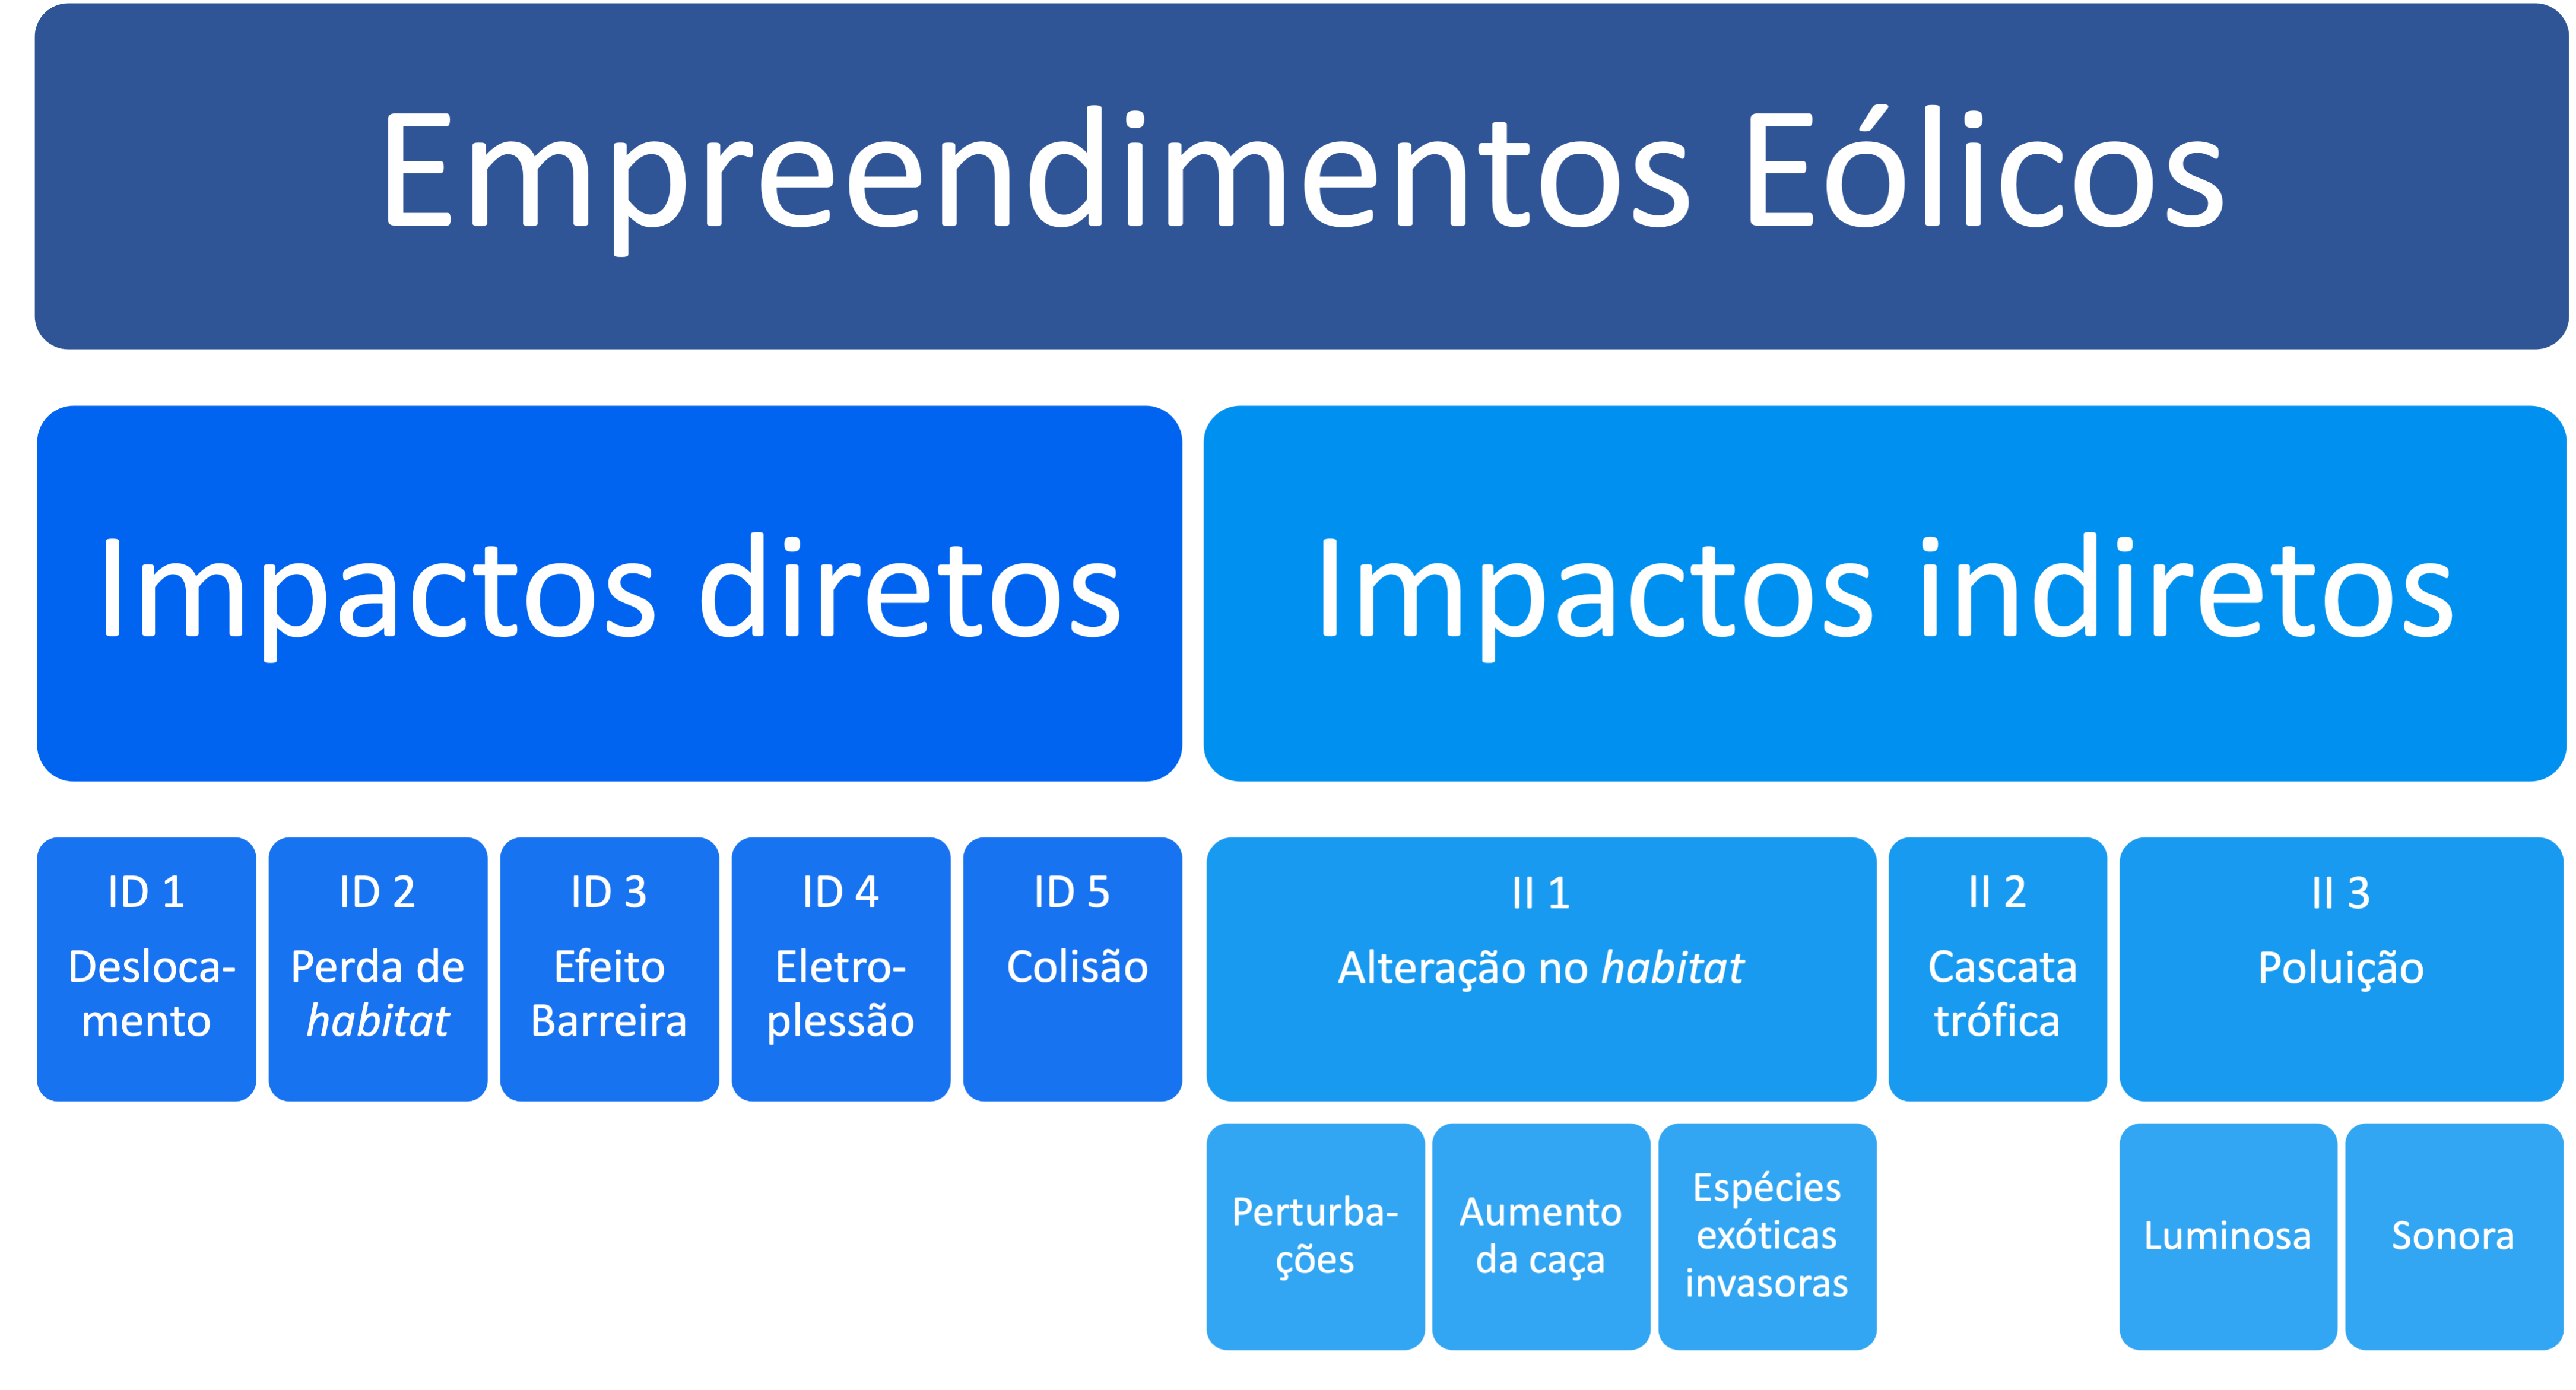
\includegraphics[width=0.75\linewidth]{imagens/cap05/Figura_5.1} 

}

\caption{Principais impactos, diretos e indiretos, observados nas diferentes fases de um empreendimento eólico (adaptado de Gode 2020). Os códigos formados por letras e números correspondem aos códigos utilizados na descrição dos  impactos  no capítulo anterior.}\label{fig:16}
\end{figure}

\hypertarget{medidas-de-mitigauxe7uxe3o-dos-principais-impactos-diretos}{%
\section{Medidas de mitigação dos principais impactos diretos}\label{medidas-de-mitigauxe7uxe3o-dos-principais-impactos-diretos}}

Este tópico traz diversas medidas de mitigação que devem ser consideradas. Entretanto, não é possível definir, neste relatório, padrões de deslocamento, períodos de ocorrência de espécies migratórias e forma de uso do habitat em um nível local. Muitas medidas propostas precisam adequar-se ao contexto da área onde será implantado o empreendimento e, para tanto, são essenciais estudos \emph{in loco} na fase de planejamento do empreendimento que indiquem as espécies sensíveis, a época de sua ocorrência no local, as rotas e corredores utilizados na área e demais aspectos relevantes para a implantação das medidas mitigadoras.

\textbf{ID 1. Deslocamento e ID 2. Perda de \emph{habitat} }

Fase do empreendimento: Construção, Operação e Descomissionamento

\begin{itemize}
\tightlist
\item
  Considerar um cronograma progressivo de intervenções físicas, com controle operacional para restauração dos danos das intervenções temporárias e redução de impactos;
\item
  Investir em ações pró-ativas de conservação, tais como a criação ou melhoria de habitat alternativos já na fase de construção;
\item
  Considerar, durante a fase de construção, a possibilidade de alteração física do projeto com a adoção de novos desenhos e estruturas a partir da identificação de oportunidades de minimização dos impactos identificados após o início da construção;
\item
  Evitar a construção de empreendimentos eólicos em áreas que possam ser, em escala local, corredores para o deslocamento de aves entre zonas florestais ou áreas úmidas (banhados);
\item
  Programar as atividades de construção de forma a evitar os períodos sensíveis para a fauna (períodos reprodutivos e de agregação, por exemplo).
\end{itemize}

\textbf{ID 3. Efeito de barreira}

Fase do empreendimento: Construção e Operação

\begin{itemize}
\tightlist
\item
  Adotar uma distância mínima entre os aerogeradores na área do parque eólico de modo a reduzir as barreiras físicas para as aves;
\item
  Adotar um alinhamento paralelo dos aerogeradores (ao invés de um alinhamento perpendicular) em relação às principais direções de deslocamento das aves, sejam elas rotas de migração, deslocamento entre dormitório e área de alimentação, entre outros;
\item
  Adotar uma distribuição de aerogeradores (\emph{layout}) de modo que se permita a formação de corredores que possam fornecer espaço seguro para a passagem das aves;
\item
  Considerar outros parques eólicos instalados nas proximidades, de modo que esses corredores de passagem possam ser formados entre parques eólicos de uma mesma região.
\end{itemize}

\textbf{ID 4. Eletroplessão e ID 5. Colisão}

\begin{verbatim}
Fase do empreendimento: Operação  
\end{verbatim}

\begin{itemize}
\tightlist
\item
  Gerenciar ativamente as turbinas. O gerenciamento ativo de turbinas (\emph{cut-in wind speeds}, \emph{curtailment} e \emph{shut-down}) deve ser considerado em áreas ou períodos críticos como parte da estratégia de mitigação. Entende-se por período crítico aquele em que há situações de alto risco de colisão, provocadas por condições climáticas ou por comportamentos específicos das aves de interesse para a conservação. Esta medida é apontada por Marques et al.~(2014), como a mais eficiente para minimizar as colisões. Desligar as turbinas temporariamente quando uma espécie de interesse está sob risco pode ser feito para períodos programados e predefinidos do dia/noite de acordo com picos de atividade das espécies, ou sazonalmente durante temporadas de migração;
\item
  Aumentar a visibilidade as pás da turbina: pintar uma lâmina da turbina. McIsaac (2001, \emph{in} Drewitt \& Langston 2006) aponta que os padrões de alto contraste podem ajudar a reduzir o risco de colisão (pelo menos em condições de boa visibilidade). Outra possibilidade sugerida, mas não testada, é a pintura das lâminas com tinta UV, o que pode aumentar sua visibilidade para as aves (Drewitt \& Langston 2006);
\item
  Instalar dispositivos sinalizadores e desviadores de voo (bolas ou espirais) nas linhas de transmissão;
\item
  Evitar criar artificialmente ambientes que possam atrair aves como alagados, estruturas que sirvam de poleiro (neste sentido, a própria nacele pode ser um atrativo) ou para nidificação. Pilhas de pedras já foram reportadas como atrativo para aves em parques eólicos, visto abrigarem potenciais presas (Drewitt \& Langston 2008);
\item
  Evitar o \emph{free-wheeling} (situação em que não há geração de energia devido à pequena velocidade do vento, mas as pás permanecem em movimento). Lâminas que giram lentamente ou com velocidade intermediária estão associadas ao maior número de colisões fatais em aves de rapina (Drewitt \& Langston 2008);
\item
  Manter corredores livres de turbinas para permitir o movimento de aves migratórias ou aves de longo deslocamento entre sítios de alimentação e descanso, a fim de evitar o efeito barreira. Esta medida deve ser prevista em grandes parques eólicos contíguos ou complexos eólicos;
\item
  Acompanhar, e adotar sempre que possível, o desenvolvimento tecnológico de dispositivos que promovam um eficiente afugentamento da fauna;
\item
  Manter o parque eólico e seus acessos (vetor de atropelamentos) livres de carcaças, inclusive as de animais domésticos. A presença de carcaças de animais pode ser um atrativo para espécies necrófagas, como urubus e carcarás. Essa situação pode ser bastante comum em locais onde os aerogeradores compartilham espaço com a pecuária;
\item
  Buscar uma configuração (\emph{layout}) do parque eólico que minimize os impactos sobre as espécies, em especial no que diz respeito ao número, tamanho e disposição dos aerogeradores. Considerando a mesma quantidade total de geração de energia, aerogeradores maiores, se em menor número, podem ser ambientalmente mais interessantes (Drewitt \& Langston 2008);
\item
  Dar atenção especial ao planejamento das linhas de transmissão, adotando uma configuração de cabos mais segura nas linhas de transmissão e fios. A morte por colisão ou eletroplessão com cabos e fiações, dada a intensidade destes elementos na paisagem, pode ser muito maior que aquela provocada por aerogeradores (e.g., Lucas et al.~2004, Biasotto \& Kindel 2018).
\end{itemize}

Biasotto et al.~(2021) modelaram o risco de eletroplessão de diferentes espécies da avifauna brasileira de forma a identificar as que necessitam de maior atenção para medidas de mitigação, e apontam que diferentes medidas mitigadoras, visando minimizar o risco de colisões, têm sido propostas. Entre essas medidas temos o replanejamento da localização de linhas de energia para formar corredores de voo, instalação de cabos subterrâneos, alterações no desenho de torres, linhas de energia com diferentes níveis de cabos para-raios ou a remoção dos mesmos e a sinalização de cabos para-raios com diferentes dispositivos. Contudo, com respeito aos sinalizadores, estes autores apontam que nenhum marcador foi igualmente eficaz para todas as espécies ou situações. A melhor solução é, sempre que possível, optar por cabos subterrâneos. Alternativamente, Dwyer et al.~(2019) reportam o uso de um sistema para evitar a colisão aviária que inclui iluminação com luz ultravioleta próxima (UV-A, ondas de 320-400 nm). Essa faixa de luz não é visível para os seres humanos, mas é visível para muitos grupos de aves e morcegos. Para um mesmo período de monitoramento, foram registradas 49 colisões com as luzes desligadas e uma única colisão com as luzes ligadas. Todas as colisões ocorreram durante a noite.

\begin{itemize}
\tightlist
\item
  Adicionar isolamento aos postes e fios para reduzir o risco de eletroplessão, bem como alterar a disposição dos fios a fim de aumentar a distância entre eles.
\end{itemize}

Um exemplo disso é a configuração triangular (Figura \ref{fig:17}), com distância segura entre os fios, adotada pela Companhia de Eletricidade do Estado da Bahia - COELBA na região de ocorrência da arara-azul-de-lear (\emph{Anodorhynchus leari}). Outras medidas que podem ser adotadas são: (i) reduzir o número de níveis verticais de fios, ajustando as alturas do condutor para reduzir o número de pontos potenciais de colisão; (ii) amarrar os fios o mais baixo possível; (iii) usar fios com diâmetro espesso ou agrupar fios para aumentar sua visibilidade, pois as aves geralmente aumentam sua altura de voo, desviando dos fios, quando os veem.

\begin{itemize}
\tightlist
\item
  Afugentar as aves. Embora as estratégias de afugentamento ainda precisem ser aprimoradas, um recurso que parece ter grande potencial é aquele baseado em sons ``desagradáveis'' para as aves, disparados por sensores de aproximação (Marques et al.~2014).
\end{itemize}

Por fim, apenas em posse de fartas e precisas informações será possível que o Brasil galgue patamares de excelência em geração de energia e proteção da biodiversidade. Considerando a expressiva quantidade de dados sobre aves que têm sido gerada nos parques eólicos brasileiros, a sua sistematização e compartilhamento em uma plataforma de fácil e livre acesso é de grande interesse para os órgãos gestores, para o mundo acadêmico e para o setor produtor de energia.

\begin{figure}

{\centering 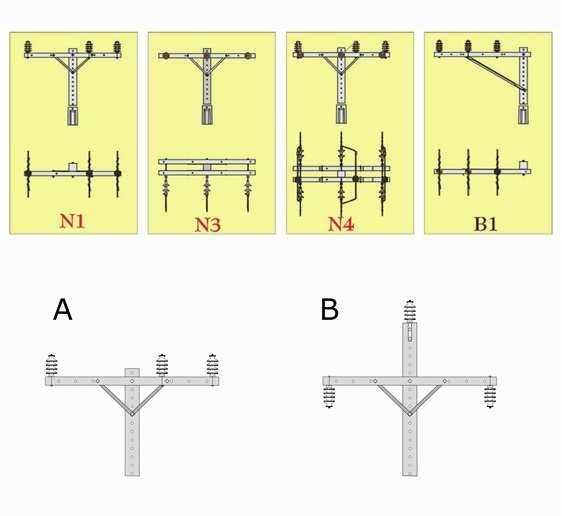
\includegraphics[width=0.75\linewidth]{imagens/cap05/Figura_5.2} 

}

\caption{Padrões de cruzetas normalmente utilizados em linhas de transmissão de energia elétrica. Exemplo de modificação de estrutura de fixação a partir da figura A para a B com aumento da distância dos fios e inversão de pontos de fixação dos condutores.}\label{fig:17}
\end{figure}

\hypertarget{medidas-de-mitigauxe7uxe3o-dos-principais-impactos-indiretos}{%
\section{Medidas de mitigação dos principais impactos indiretos}\label{medidas-de-mitigauxe7uxe3o-dos-principais-impactos-indiretos}}

\textbf{II 1. Alteração no \emph{habitat} }

\begin{verbatim}
Fase do empreendimento: Construção, Operação e Descomissionamento  
\end{verbatim}

\begin{itemize}
\tightlist
\item
  Implantar um programa de vigilância que restrinja a circulação de pessoas não autorizadas pelos acessos internos do empreendimento a fim de evitar o molestamento, a caça e a apanha de espécimes da fauna;
\item
  Revegetar áreas de uso temporário conforme forem disponibilizadas, usando cobertura de solo e plantas nativas do local, sempre que possível;
\item
  Adotar medidas para controle dos processos erosivos, mantendo no plano de gestão ambiental do empreendimento as ações previstas para a redução dos impactos, particularmente dos processos erosivos e de contaminações do solo, tanto no período de construção quanto na operação do empreendimento.
\end{itemize}

\textbf{II 2. Cascata trófica}

\begin{verbatim}
Fase do empreendimento: Construção, Operação e Descomissionamento  
\end{verbatim}

\begin{itemize}
\tightlist
\item
  Realizar monitoramentos da mortalidade de aves em longo prazo. Tendo em vista que a natureza e a prevalência desse impacto ainda são pouco compreendidas, não é possível sugerir medidas mitigadoras nesse momento. Assim sendo, é essencial o acúmulo de dados que permitam avaliar este impacto e planejar medidas que o minimizem.
\end{itemize}

\textbf{II 3. Poluição}

\begin{verbatim}
Fase do empreendimento: Construção, Operação e Descomissionamento  
\end{verbatim}

\begin{itemize}
\tightlist
\item
  Programa de redução de ruídos;
\item
  Estabelecer controle gerencial das atividades contratadas, sinalizando ou delimitando áreas sensíveis e restritas ao acesso de pessoas e maquinários;
\item
  Limitar a instalação de luzes sinalizadoras ao mínimo necessário ou usar luzes intermitentes (estroboscópicas) vermelhas.
\end{itemize}

Embora parques eólicos terrestres não sejam a única fonte luminosa na paisagem, são esperadas eventuais perturbações sobre a avifauna. Mesmo que não seja consenso entre a comunidade científica (e.g., Evans et al.~2007, Poot et al.~2008), estudos mais atuais (Gehring et al 2009, Kerlinger et al.~2010) sugerem que as turbinas eólicas devem ser equipadas somente com luzes intermitentes e preferencialmente de cor vermelha. Sensores de aproximação poderiam reduzir a necessidade de luzes sinalizadoras. O tipo de iluminação e a sinalização luminosa a serem adotadas em um parque eólico estão sujeitas a regulamentações relacionadas, por exemplo, à aviação civil. Por isso, esta discussão deve ser fomentada e compartilhada com todos os setores da sociedade e governo envolvidos, principalmente quando se considera que a opção \emph{offshore} para parques eólicos começa a ser uma realidade no país.

Este capítulo apresentou diversas medidas de mitigação encontradas em literatura. Muitas já foram testadas e aprovadas, mas a maioria delas em outros países, com clima e relevo diferentes do nosso e um conjunto de espécies também bastante diferente. Ter essas experiências à disposição nos dá um ponto de partida importante para as boas práticas em relação a aves em empreendimentos eólicos no Brasil. No entanto, considerando que a efetividade de medidas de mitigação depende do contexto local (fatores abióticos e espécies envolvidas), é indispensável que haja um monitoramento criterioso dos efeitos das medidas implantadas. Os resultados de tal monitoramento, positivos ou negativos, devem ser analisados e divulgados para que possamos avançar no conhecimento do tema em nosso país e aprimorar as recomendações dentro da nossa realidade. Isso permitirá que investimentos futuros em medidas de mitigação nas diferentes regiões brasileiras sejam feitos com maior precisão e melhores resultados, gerando economia de recursos e reduzindo os impactos na biodiversidade.

\hypertarget{referuxeancias-bibliogruxe1ficas-4}{%
\section{Referências bibliográficas}\label{referuxeancias-bibliogruxe1ficas-4}}

Atienza, J.C., Martín, I., Infante, O., Valls, J. 2011. Directrices para la evaluación del impacto eólico en aves y murciélagos. SEO/BirdLife, Madrid, 53p. Disponível em: \url{https://www.seo.org/wp-content/uploads/2012/05/MANUAL-MOLINOS-VERSION-31_WEB.pdf} Acesso em: {[}17/03/2022{]}.

Bennun, L., van Bochove, J., Ng, C., Fletcher, C., Wilson, D., Phair, N., Carbone, G. 2021. Mitigating biodiversity impacts associated with solar and wind energy development: guidelines for project developers. IUCN/The Biodiversity Consultancy. Gland/Cambridge. \url{https://doi.org/10.2305/IUCN.CH.2021.04.en}

Biasotto, L.D., Kindel, A. 2018. Power lines and impacts on biodiversity: A systematic review. Environmental Impact Assessment Review 71: 110-119. \url{https://doi.org/10.1016/j.eiar.2018.04.010}

Biasotto, L. D., Moreira, F., Bencke, G. A., D'Amico, M., Kindel, A., Ascensão, F. 2021. Risk of bird electrocution in power lines: a framework for prioritizing species and areas for conservation and impact mitigation. Animal Conservation \url{https://doi.org/10.1111/acv.12736}

BirdLife International. 2014. Important Bird and Biodiversity Areas: A global network for conserving nature and benefiting people. BirdLife International. Cambridge. Disponível em: \url{https://www.birdlife.org/papers-reports/important-bird-and-biodiversity-areas-a-global-network-for-conserving-nature-and-benefiting-people-2014} Acesso em: {[}22/02/2022{]}.

Bridgewater, P., Kim, R.E. 2021. The Ramsar Convention on Wetlands at 50. Nature Ecology \& Evolution 5: 268--270. \url{https://doi.org/10.1038/s41559-021-01392-5}

De Lucas, M., Janss, G.F.E., Ferrer, M. 2004. The effects of a wind farm on birds in a migration point: the Strait of Gibraltar. Biodiversity Conservation 13: 395--407. \url{https://doi.org/10.1023/B:BIOC.0000006507.22024.93}

Donald, P., Fishpool, L., Ajagbe, A., Bennun, L., Bunting, G., Burfield, I. et al.~2019. Important Bird and Biodiversity Areas (IBAs): The development and characteristics of a global inventory of key sites for biodiversity. Bird Conservation International 29(2): 177-198. \url{https://doi.org/10.1017/S0959270918000102}

Drewitt, A.L., Langston, R.H.W. 2006. Assessing the impacts of wind farms on birds. Ibis 148: 29--42. \url{https://doi/10.1111/j.1474-919X.2006.00516.x}

Drewitt, A.L., Langston, R.H.W. 2008. Collision effects of wind-power generators and other obstacles on birds. Annals of the New York Academy of Sciences 1134: 233--266. \url{https://doi.org/10.1196/annals.1439.015}

Dwyer, J.F., Pandey, A.K., McHale, L.A., Harness, R.E. 2019. Near-ultraviolet light reduced Sandhill Crane collisions with a power line by 98\%. Condor 121: 1--10. \url{https://doi.org/10.1093/condor/duz008}

Evans, W.R., Akashi Y., Altman N.S., Manville, A.M. 2007. Response of night-migrating songbirds in cloud to colored and flashing light. North American Birds 60(4): 476-488 Disponível em: \url{https://www.researchgate.net/publication/303170066_Response_of_night-migrating_songbirds_in_cloud_to_colored_and_flashing_light} Acesso em: {[}17/03/2022{]}.

Gehring, J., Kerlinger, P., Manville, A.M. 2009. Communication towers, lights, and birds: successful methods of reducing the frequency of avian collisions. Ecological Applications 19(2): 505-514. \url{https://doi.org/10.1890/07-1708.1}

Gode, P. 2020. How to design future wind farms to best mitigate their disturbance effects on birds? Master's dissertation. Department of Civil \& Environmental Engineering. University of Strathclyde. \url{https://doi.org/10.13140/RG.2.2.18138.36808}
IUCN (International Union for Conservation of Nature). 2020. Guidelines for using a global standard for the identification of Key Biodiversity Areas: version 1.1. IUCN, International Union for Conservation of Nature. Disponível em: \url{https://portals.iucn.org/library/node/49131} Acesso em: {[}17/03/2022{]}.

Kerlinger, P., Gehring, J.L., Erickson, W.P., Curry, R., Jain, A., Guarnaccia, J. 2010. Night migrant fatalities and obstruction lighting at wind turbines in North America. The Wilson Journal of Ornithology 122(4): 744-754. \url{http://dx.doi.org/10.1676/06-075.1}

Marques, A.T., Batalha, H., Rodrigues, S., Costa, H., Pereira, M.J.R., Fonseca, C., Mascarenhas, M., Bernardino, J. 2014. Understanding bird collisions at wind farms: An updated review on the causes and possible mitigation strategies. Biological Conservation 179: 40--52. \url{https://doi.org/10.1016/j.biocon.2014.08.017}

Metternicht, G. 2018. Land use and spatial planning: Enabling sustainable management of land resources. Springer.

PNRS (Política Nacional de Resíduos Sólidos). 2010. Lei nº 12.305, de 2 de agosto de 2010. Institui a Política Nacional de Resíduos Sólidos.

Poot, H., Ens, B.J., de Vries, H., Donners, M.A.H., Wernand, M.R., Marquenie, J.M. 2008. Green light for nocturnally migrating birds. Ecology and Society 13(2): 47. Disponível em: \url{http://www.ecologyandsociety.org/vol13/iss2/art47/} Acesso em: {[}22/02/2022{]}.

Ramsar Convention Secretariat. 2013. The Ramsar Convention Manual: a guide to the Convention on Wetlands (Ramsar, Iran, 1971), 6th ed.~Ramsar Convention Secretariat. Gland. Disponível em: \url{https://www.ramsar.org/sites/default/files/documents/library/manual6-2013-e.pdf} Acesso em: {[}22/02/2022{]}.

Rebke, M., Dierschke, V., Weiner, C.N., Aumüller, R., Hill, K., Hill, R. 2019. Attraction of nocturnally migrating birds to artificial light: The influence of colour, intensity and blinking mode under different cloud cover conditions. Biological Conservation 233: 220--227. \url{http://dx.doi.org/10.1016/J.BIOCON.2019.02.029}

\hypertarget{cap6}{%
\chapter{\texorpdfstring{Reflexões sobre o monitoramento de aves em empreendimentos eólicos \emph{onshore}}{Reflexões sobre o monitoramento de aves em empreendimentos eólicos onshore}}\label{cap6}}

\pagestyle{headings}

\textbf{Ivan Braga Campos\textsuperscript{1} \& Marcos de Souza Fialho\textsuperscript{2}}

\emph{1. Parque Nacional da Serra do Cipó}\\
\emph{Instituto Chico Mendes de Conservação da Biodiversidade - ICMBio}\\
\emph{Rodovia MG-10 Km 94}\\
\emph{35847-000 Jaboticatubas, MG}

\emph{2. Centro Nacional de Pesquisa e Conservação de Aves Silvestres -- CEMAVE}\\
\emph{Instituto Chico Mendes de Conservação da Biodiversidade - ICMBio}\\
\emph{Floresta Nacional da Restinga de Cabedelo}\\
\emph{BR-230 Km 10}\\
\emph{58108-012 Cabedelo, PB}

Iniciativas de monitoramento comumente têm como objetivo medir estados e tendências da biodiversidade (Lee et al.~2005). O monitoramento eficaz, na perspectiva conservacionista, é aquele que nos permite avaliar as respostas de populações e ecossistemas às práticas de conservação e aos impactos das diversas atividades humanas.

No caso do monitoramento de impactos, um bom monitoramento deve ser capaz de informar a respeito do resultado das intervenções realizadas e das medidas de mitigação adotadas sobre as populações das espécies que vivem ou usam determinado local ou recurso.

É de se esperar que diferentes intervenções inerentes a diferentes tipologias de empreendimentos tenham impactos variados sobre espécies de grupos taxonômicos distintos, de acordo com a biologia de cada grupo e espécie. Dessa forma, o monitoramento de impactos tende a sofrer uma especialização de acordo com a tipologia do empreendimento. E para cada tipologia a padronização de métodos e métricas se faz necessária para a geração de dados e informações comparáveis entre empreendimentos, permitindo um melhor entendimento do que acontece em diferentes escalas temporais e espaciais (local, regional, nacional etc.), bem como de seus efeitos sinérgicos e cumulativos. Em última instância, esta padronização permite uma otimização dos esforços do próprio setor público relacionados ao licenciamento e controle das atividades impactantes.

No entanto, em meio a todos os ritos processuais, padrões estabelecidos e métodos de monitoramento usuais, é importante não perdermos de vista que o grande objetivo de um monitoramento de biodiversidade é medir estados e tendências de populações e ecossistemas. Quando associado a processos de licenciamento ambiental, busca-se também avaliar a eventual relação dos estados e tendências revelados pelo monitoramento com os impactos da instalação e operação do empreendimento em questão. Desenhos amostrais que desconsideram o estado das populações antes de um determinado impacto dificilmente possibilitarão correlacionar eventuais alterações de estados e tendências a impactos do empreendimento ou permitirão inferências sobre a efetividade das medidas mitigadoras adotadas.

Essa reflexão não traz respostas simples, considerando os limites temporais estabelecidos para os ritos processuais de licenciamento. Porém, é uma perspectiva necessária para que o monitoramento não se torne um fim em si mesmo e para se evitar esforços na geração de dados que pouco poderão contribuir para responder às questões motivadoras do monitoramento proposto.

\hypertarget{por-que-monitorar-a-biodiversidade-em-parques-euxf3licos}{%
\section{Por que monitorar a biodiversidade em parques eólicos?}\label{por-que-monitorar-a-biodiversidade-em-parques-euxf3licos}}

A permanente preocupação acerca dos impactos da instalação e funcionamento de parques e complexos eólicos sobre a biodiversidade é relevante e necessária. O monitoramento dos impactos desse tipo de atividade contribuirá, em última instância, para garantir a harmonização entre a geração de energia e a manutenção da biodiversidade brasileira, agregando ainda mais valor ao conceito de sustentabilidade já associado aos empreendimentos eólicos.

O monitoramento torna-se ainda mais relevante quando os empreendimentos estão localizados em unidades de conservação, ainda que seja permitida a instalação de parques eólicos, se compatível com os objetivos de criação da unidade. É o caso das Áreas de Proteção Ambiental (APA), categoria de unidade de conservação de uso sustentável prevista no SNUC (Sistema Nacional de Unidades de Conservação, Lei nº 9.985/2000).

Cabe destacar que o Brasil é signatário da Convenção sobre a Conservação das Espécies Migratórias de Animais Silvestres (CMS, do inglês \emph{Convention on Migratory Species}) e sua Resolução nº 7.5 trata do compromisso do país em envidar esforços para a conciliação entre a exploração do potencial eólico e a conservação deste recorte da biodiversidade de interesse global e potencialmente vulnerável a esse tipo de atividade.

Na geração de energia por parques eólicos \emph{onshore} (em contraposição aos \emph{offshore}) a biota terrestre seria a mais vulnerável, principalmente pela supressão vegetal decorrente da abertura de vias de acesso, pela intensificação do tráfego, pela instalação de torres e redes de transmissão e de distribuição, dentre outras atividades (Figura \ref{fig:18}). As linhas de transmissão, de distribuição e as torres geradoras de energia, também chamadas turbinas ou aerogeradores, afetam principalmente as comunidades de aves e morcegos (Choi et al.~2020). Salienta-se que as mortes ou lesões por colisão em aves e morcegos constituem o impacto mais conspícuo, despertando grande interesse da sociedade em geral.

\begin{figure}[H]

{\centering 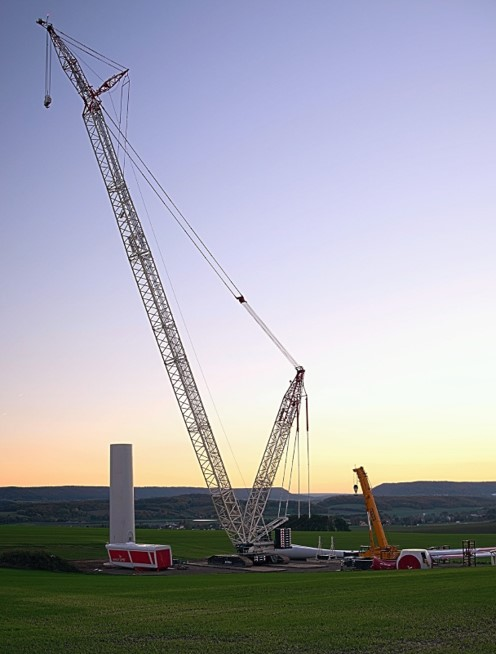
\includegraphics[width=0.5\linewidth]{imagens/cap06/Figura_6.1} 

}

\caption{Montagem de um aerogerador ou turbina eólica. Fonte: Pixabay.com}\label{fig:18}
\end{figure}

Todavia, diferentes espécies de aves respondem de forma distinta aos parques eólicos, sendo essa resposta também condicionada por fatores climáticos, condições ambientais locais, como relevo e vegetação e, ainda, pela gestão e manejo do parque. A extensão do impacto irá variar também conforme a espécie, a estação, a localização e o \emph{layout} ou configuração dos empreendimentos. Esses impactos podem ser permanentes ou temporários, ocorrendo nas fases de implantação, operação e descomissionamento do empreendimento, com impactos característicos de cada fase (veja Figura 4.1). O capítulo 4 aponta para perda de \emph{habitat}, efeito de barreira, deslocamento, electrocussão e colisão como sendo impactos diretos, enquanto poluição e alterações no \emph{habitat} e na cascata trófica são considerados impactos indiretos. Dentre os impactos diretos à fauna, qualquer ave com potencial de voo se torna vulnerável a colisões. No entanto, é sabido que características como tamanho corporal, morfologia, comportamento, tipo de voo e grupo a qual pertencem são fatores que influenciam no risco de colisão de cada espécie. Para maiores detalhes veja capítulo 4.

O monitoramento deve ser capaz de avaliar a magnitude dos distintos impactos à fauna, sejam diretos ou indiretos (barreira, deslocamento) e a efetividade das medidas mitigadoras adotadas, gerando informações que contribuam para uma melhor gestão do parque (Smallwood 2017, Bennun et al.~2021) (Figura \ref{fig:19}).

\begin{figure}

{\centering 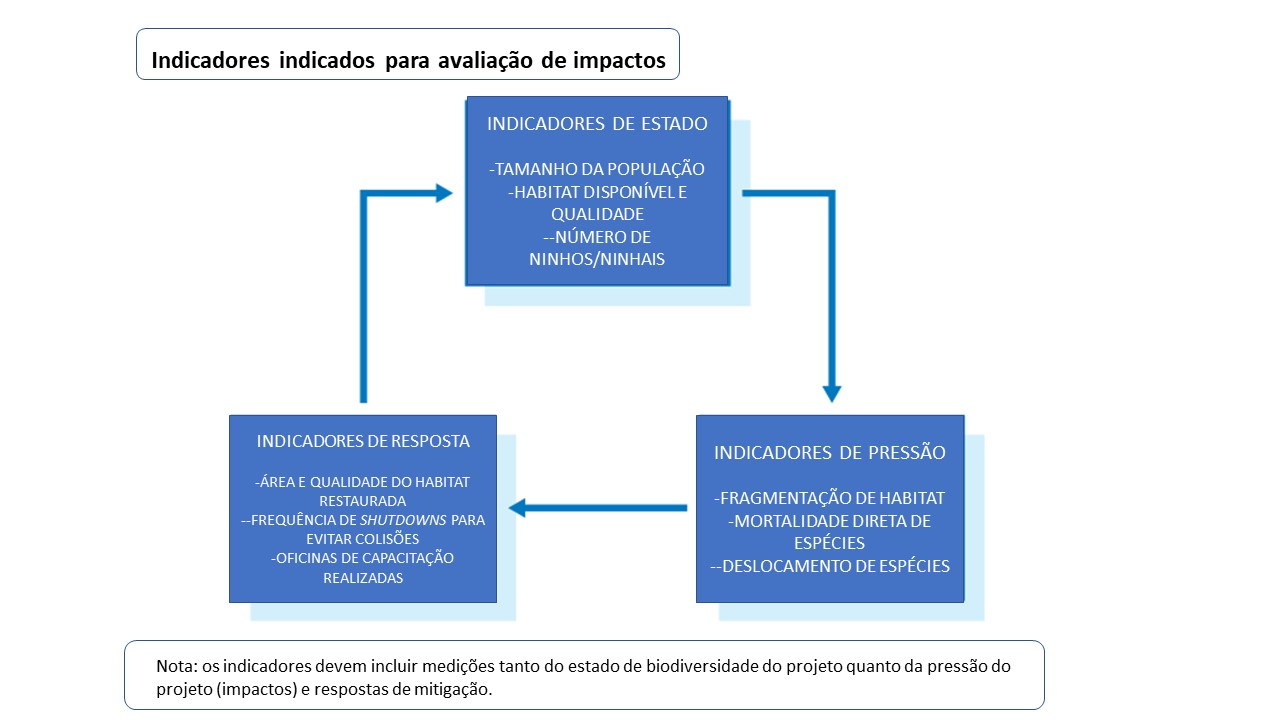
\includegraphics[width=0.85\linewidth]{imagens/cap06/Figura_6.2} 

}

\caption{Exemplo de interação entre monitoramento e gestão de conflitos. Adaptado de: Bennun et al. (2021)}\label{fig:19}
\end{figure}

Em paisagens muito dinâmicas, como aquelas dominadas por lavouras de arroz, por exemplo, onde as práticas agrícolas influenciam a abundância de aves limícolas e aquáticas, além da sazonalidade é importante que as amostragens contemplem as diferentes fases do uso do solo ou os diferentes estágios de ocupação ao longo do tempo.

Por fim, o monitoramento gera dados para o aprimoramento dos modelos de risco de colisão, que buscam predizer a taxa de colisão de um táxon com determinadas estruturas. Atualmente, os modelos de risco de colisão disponíveis possibilitam considerar numerosas variáveis, desde características espécie-específicas de voo à configuração do parque eólico (Marques et al.~2014, Laranjeiro et al.~2018).

\hypertarget{a-importuxe2ncia-dos-estudos-tipo-baci}{%
\section{A importância dos estudos tipo BACI}\label{a-importuxe2ncia-dos-estudos-tipo-baci}}

Um princípio recomendado na literatura científica para o monitoramento é que o delineamento amostral seja do tipo BACI (\emph{before and after -- control impact}), que envolve a avaliação de impactos ou a caracterização do cenário ambiental antes e depois do empreendimento (Kuvlesky et al.~2007). A padronização de métodos para o diagnóstico ambiental e especialmente para o monitoramento é desejável, a fim de criar um conjunto de dados estatisticamente comparável em diferentes escalas temporais e espaciais (Paton et al.~2017). Ou seja, a definição de métodos e métricas durante o estudo de impacto ambiental deve estar alinhada aos objetivos e métodos a serem empregados no monitoramento a ser realizado durante a fase de operação.

Neste contexto, amostragens ou mesmo experimentos prévios que avaliem, por exemplo, a taxa local de remoção de carcaças são muito pertinentes, visto que altas taxas de remoção podem mascarar a magnitude das taxas de colisão. Não havendo a possibilidade ou existência de dados prévios, áreas controle com indicadores ambientais compatíveis podem ser estabelecidas de forma a mitigar essa lacuna de dados sobre taxa local de remoção de carcaças.

Considerando a longa vida útil destes empreendimentos, o monitoramento também deve ser flexível, de modo que os monitores possam incluir protocolos que foquem em espécies e métodos originalmente não previstos, de forma a considerar problemas que venham a ser constatados apenas após a implantação do empreendimento.

\hypertarget{muxe9todos-correntes-e-questuxf5es-a-serem-respondidas-pelo-monitoramento}{%
\section{Métodos correntes e questões a serem respondidas pelo monitoramento}\label{muxe9todos-correntes-e-questuxf5es-a-serem-respondidas-pelo-monitoramento}}

Como já mencionado, tanto a magnitude dos distintos impactos à fauna, sejam diretos ou indiretos, quanto a efetividade das medidas mitigadoras adotadas devem ser contempladas pelo monitoramento, proporcionando subsídios à gestão do parque (Smallwood 2017, Bennun et al.~2021).

Os protocolos empregados para o monitoramento da ocorrência e uso do espaço por aves nos parques eólicos, assim como dos impactos desses empreendimentos sobre esse grupo animal ainda são relativamente simples no Brasil, consistindo em observações de campo e métodos clássicos da ornitologia, como ponto de escuta, listas de Mackinnon e uso de redes de neblina, somados ao monitoramento de carcaças (Figura \ref{fig:20}). No entanto, novas tecnologias que permitem o monitoramento remoto, contínuo, mesmo durante a noite, e em tempo real, a despeito das condições climáticas, despontam como alternativas interessantes, ainda mais quando se considera que os monitoramentos correntes nos parques eólicos do país tendem a ser concentrados em curtos períodos de alguns dias, espaçados por vários meses. Dentre essas tecnologias de monitoramento remoto temos: câmeras de vídeo, radares verticais e horizontais, sistemas de detecção termais baseados em câmeras de infravermelho, sensores acústicos e de pressão, essenciais para o monitoramento de parques \emph{offshore}, dado o contexto em que se inserem (Desholm et al.~2004, Walls et al.~2009, Wang et al.~2015), mas que também devem ser aplicadas no monitoramento \emph{onshore}, devido às inúmeras vantagens citadas acima.

\begin{figure}[H]

{\centering 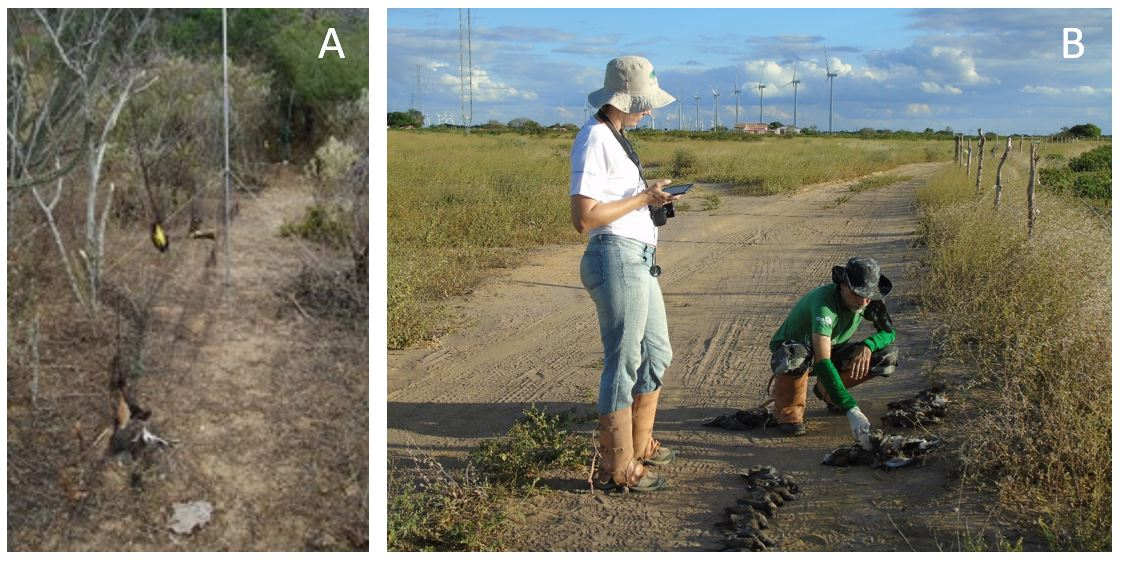
\includegraphics[width=0.75\linewidth]{imagens/cap06/Figura_6.3ab} 

}

\caption{A. Captura por rede de neblina; B. Busca ativa por aves mortas por colisão e eletroplessão. Fotos: Emanuel Sousa e Flávia Regina Domingos}\label{fig:20}
\end{figure}

Idealmente, além de apresentar um esforço amostral suficiente, o monitoramento deve ser temporalmente distribuído de modo a contemplar a sazonalidade local e incorporar dados meteorológicos. Variações nos resultados do monitoramento são esperadas tanto por questões climáticas, como a presença de nevoeiros ou a intensidade de ventos, quanto por questões biológicas e ecológicas das espécies, como a maior movimentação e as alterações no padrão de forrageamento na estação reprodutiva, o deslocamento de migratórias (ida e retorno dos sítios de invernada) ou a inexperiência de imaturos.

A habituação das aves às estruturas dos empreendimentos eólicos, em especial aos aerogeradores, ainda é pouco compreendida e alvo de debate (Masden et al.~2010). Há controvérsias entre diferentes estudos. Alguns apontam que não haveria um aumento da mortalidade, com o passar dos anos, em espécies que habitam os parques eólicos, enquanto outros argumentam que, passado o efeito inicial de afastamento das aves da área do empreendimento (deslocamento), poderia haver uma eventual habituação e reocupação da área, levando a um incremento na mortalidade por colisões (veja capítulo 4).

Num parque ou complexo eólico é esperado que alguns aerogeradores respondam significativamente por mais fatalidades. Portanto, quando da implantação de um novo empreendimento, é fundamental o acompanhamento contínuo do desempenho de cada aerogerador, a fim de identificar aqueles mais fatais e, a partir deste reconhecimento, adotar medidas mitigadoras. Em casos extremos, com prejuízos relevantes a populações de espécies de especial interesse para a conservação, deveria ser considerada inclusive a realocação ou inativação do aerogerador.

Naturalmente, no monitoramento deve-se dar especial atenção para as espécies ameaçadas ou com problemas locais de conservação, mas sem ignorar os demais componentes da comunidade.

Por fim, o esforço ideal de monitoramento tende a apresentar uma correlação positiva com a dimensão do empreendimento já que grandes empreendimentos podem representar barreiras significativas para as aves, além de potencializar a degradação de \emph{habitat}. Da mesma forma, o esforço de monitoramento para empreendimentos localizados em uma área onde há outros empreendimentos instalados deve considerar os efeitos cumulativos do conjunto de empreendimentos. Para um maior detalhamento sobre os métodos correntes em monitoramentos \emph{onshore} e ponderações sobre esforços mínimos de amostragem veja Smallwood (2017).

\hypertarget{limitantes-do-monitoramento-em-parques-euxf3licos}{%
\section{Limitantes do monitoramento em parques eólicos}\label{limitantes-do-monitoramento-em-parques-euxf3licos}}

Diversos são os fatores que podem limitar o sucesso de um programa de monitoramento. Desde uma limitação orçamentária até a falta de capacitação específica no tema pelos técnicos responsáveis. Contudo, destaca-se que a ausência de dados pretéritos à construção do empreendimento é um dos limitantes mais óbvios. O Serviço de Pesca e Vida Selvagem Estadunidense (\emph{U.S. Fish and Wildlife Service}) estima que são necessários três anos de acompanhamento para a determinação de picos de abundância de aves (Smallwood 2017).

Os esforços de campo têm sido, de modo geral, bastante modestos e, talvez, a consequência mais séria ocasionada por um esforço amostral limitado seja não gerar resultados confiáveis e estatisticamente significativos. Destaca-se, também, a ausência de meta-análises com dados de diferentes parques localizados em uma mesma região, buscando avaliar possíveis efeitos cumulativos (Masden et al.~2010), parcialmente explicada pela inexistência de plataformas virtuais que compilam dados e informações geradas nos EIAs e outros estudos ambientais e nos monitoramentos para esta tipologia de empreendimento. No estado do Rio Grande do Sul, Falavigna et al.~(2020) buscaram, por meio de uma análise regional, padrões dos efeitos dos vários parques eólicos no litoral e na campanha gaúcha sobre a avifauna. A comunidade de aves respondeu às mudanças na paisagem, principalmente devido à redução da cobertura florestal nativa e exótica, em áreas afetadas pela instalação e operação de parques eólicos, tanto na composição das espécies quanto nas guildas ambientais. Contudo, segundo os autores, são necessários levantamentos mais detalhados e mais longos para confirmar esta tendência.

Via de regra, a maioria dos estudos foca em colisões e no efeito de deslocamento das populações e não nos efeitos comportamentais (Madders \& Whitfield 2006), que podem resultar em uma diminuição da aptidão dos indivíduos com possíveis implicações em seu sucesso reprodutivo, totalmente ignorado até então. Considerando que é uma linha de estudo pouco provável de ser abordada durante o licenciamento, a comunidade científica teria muito a contribuir.

Diante da adoção ainda incipiente de tecnologias remotas de monitoramento, as estimativas de colisão têm seus resultados fortemente influenciados pela frequência de busca por carcaças, proporção de aerogeradores vistoriados, raio de busca em relação à base do aerogerador e tipo de vegetação do local do empreendimento. Além disso, há um viés provocado pela remoção de animais moribundos ou carcaças por predadores ou espécies necrófagas, além das limitações inerentes do observador, sendo fortemente recomendado o uso de métodos alternativos a partir de radares, imagens térmicas e detecção acústica (Drewitt \& Langston 2006). Caso esses métodos não possam ser aplicados, os estudos devem estimar previamente a taxa de remoção de carcaças.

\hypertarget{boas-pruxe1ticas-para-o-monitoramento-em-parques-euxf3licos}{%
\section{Boas práticas para o monitoramento em parques eólicos}\label{boas-pruxe1ticas-para-o-monitoramento-em-parques-euxf3licos}}

Recomenda-se que os processos de licenciamento e monitoramento sejam transparentes, que o acesso de pesquisadores independentes aos empreendimentos eólicos seja facilitado e que se incentive a divulgação dos dados de estudos e monitoramentos, iniciativas que certamente contribuirão para uma melhor compreensão dos impactos e para a divulgação e adoção gradativa de melhores práticas. O compartilhamento de dados também contribui para o nivelamento de informações sobre métodos de monitoramento e medidas de mitigação bem sucedidas e possibilita análises de impactos cumulativos de diferentes empreendimentos na paisagem (Bennun et al.~2021).

O monitoramento deve buscar não somente uma quantidade de dados suficiente para as análises estatísticas pretendidas, mas também é esperado que gere dados de qualidade. Estimativas de mortes de aves por colisões são um bom exemplo. Para melhorar a qualidade dos dados, além de considerar as taxas de remoção de carcaças nos diferentes ambientes, espera-se que também sejam contabilizados fatores que já são reconhecidos por influenciar as taxas de colisão, como picos de atividades de migração, comportamento de voo de diferentes espécies de aves, condições climáticas, velocidade e direção do vento, topografia e configuração do parque eólico (Wang et al.~2015).

Uma vez que as espécies afetadas sejam identificadas e suas taxas de mortalidade obtidas, caberia avaliar se, social e ecologicamente, tal magnitude de impactos é aceitável. Não o sendo, deve o empreendedor promover adequações estruturais ou de funcionamento do parque eólico ou, ainda, devem os órgãos licenciadores se manifestar a respeito.

Pesquisas voltadas especificamente ao monitoramento dos parques eólicos também são necessárias. Espera-se que tais estudos lancem mão de uma combinação de métodos de amostragem como rede de neblina, imageamento por sensores termais, radiotelemetria, radares horizontais e verticais, monitoramento acústico e vigilância meteorológica (Wang et al.~2015). Uma melhor compreensão dos fatores envolvidos na mortalidade de aves é de interesse de pesquisadores, empreendedores e órgãos licenciadores. Dados de qualidade e pesquisas sobre o monitoramento dos parques eólicos poderão gerar subsídios para o aprimoramento dos parques eólicos e dos processos de licenciamento. Um bom exemplo de aprimoramento do funcionamento de parques eólicos é a emissão de sinais sonoros e o desligamento de aerogeradores por demanda a partir da detecção automática de aves através de análise de imagens e tecnologias de radar (Bennun et al.~2021).

O \emph{Guía de Buenas Prácticas para el Desarrollo Eólico en Argentina} (Argentina 2019) recomenda uso do \emph{software} livre GenEst (Simonis et al.~2018, GenEst 2022) para a geração de estimativas de mortalidade tanto para aves quanto para morcegos, mas para isso reforça-se a necessidade de dados robustos.

Quanto melhor a informação gerada a partir do monitoramento, maior o potencial de que seja utilizada na constante melhoria de funcionamento dos parques eólicos e no desenvolvimento de soluções tecnológicas visando menor impacto sobre as aves.

Por fim, deve-se disponibilizar às instituições de controle e gestão ambiental e, se possível, ao público em geral, toda informação atualizada produzida no âmbito do monitoramento ambiental por meio de uma interface \emph{on-line} de fácil acesso.

\hypertarget{referuxeancias-bibliogruxe1ficas-5}{%
\section{Referências bibliográficas}\label{referuxeancias-bibliogruxe1ficas-5}}

Argentina. 2019. Guía de Buenas Prácticas para el Desarrollo Eólico en Argentina: Gestión de Impactos en Aves y Murciélagos. BID, IFC \& Subsecretaría de Energías Renovables y Eficiencia Energética. Washington D.C. 87p. Disponível em: \url{https://www.argentina.gob.ar/sites/default/files/guia_buenas_practicas_energia_eolica_y_biodiversidad_-_final_web.pdf} Acesso em: {[}02/03/2022{]}.

Bennun, L., van Bochove, J., Ng, C., Fletcher, C., Wilson, D., Phair, N., Carbone, G. 2021. Mitigating biodiversity impacts associated with solar and wind energy development: guidelines for project developers. IUCN/The Biodiversity Consultancy. Gland/Cambridge. \url{https://doi.org/10.2305/IUCN.CH.2021.04.en}

Choi, D.Y., Wittig, T.W., Kluever, B.M. 2020. An evaluation of bird and bat mortality at wind turbines in the Northeastern United States. PLoS ONE 15(8): e0238034. \url{https://doi.org/10.1371/journal.pone.0238034}

Desholm, M., Fox, A. Beasley, P. 2004. Best Practice Guidance for the Use of Remote Techniques for Observing Bird Behaviour in Relation to Offshore Wind Farms (Report No.~REMOTE-05-2004). Collaborative Offshore Wind Research into the Environment (COWRIE). 93p. Disponível em: \url{https://tethys.pnnl.gov/sites/default/files/publications/Desholm-et-al-2004.pdf} Acesso em: {[}22/02/2022{]}.

Drewitt, A.L., Langston, R.H.W. 2006. Assessing the impacts of wind farms on birds. Ibis 148: 29--42. \url{https://doi/10.1111/j.1474-919X.2006.00516.x}

Falavigna, T.J., Pereira, D., Rippel, M.L., Petry, M.V. 2020. Changes in bird species composition after a wind farm installation: A case study in South America. Environmental Impact Assessment Review 83: 106387. \url{https://doi.org/10.1016/J.EIAR.2020.106387}

GenEst. 2022. A Generalized Estimator of Mortality. Disponível em: \url{https://www.usgs.gov/node/279364} Acesso em: {[}22/02/2022{]}.

Kuvlesky, W.P., Brennan, L.A., Morrison, M.L., Boydston, K.K., Ballard, B.M., Bryant, F.C. 2007. Wind energy development and wildlife conservation: Challenges and opportunities. The Journal of Wildlife Management 71(8): 2487--2498. Disponível em: \url{http://www.jstor.org/stable/4496368} Acesso em: {[}22/02/2022{]}.

Laranjeiro, T., May, R., Verones, F. 2018. Impacts of onshore wind energy production on birds and bats: recommendations for future life cycle impact assessment developments. The International Journal of Life Cycle Assessment 23(10): 2007-2023. \url{https://doi.org/10.1007/s11367-017-1434-4}

Lee, W., McGlone, M., Wright, E. 2005. A review of national and international systems and a proposed framework for future biodiversity monitoring by the Department of Conservation. Landcare Research Contract Report: LC0405/122. Wellington. 216p.

Madders, M., Whitfield, D.P. 2006. Upland raptors and the assessment of wind farm impacts. Ibis 148: 43--56. \url{https://doi.org/10.1111/j.1474-919X.2006.0}

Marques, A.T., Batalha, H., Rodrigues, S., Costa, H., Pereira, M.J.R., Fonseca, C., Mascarenhas, M., Bernardino, J. 2014. Understanding bird collisions at wind farms: An updated review on the causes and possible mitigation strategies. Biological Conservation 179: 40--52. \url{https://doi.org/10.1016/j.biocon.2014.08.017}

Masden, E.A., Fox, A.D., Furness, R.W., Bullman, R., Haydon, D. 2010. Cumulative impact assessments and bird/wind farm interactions: Developing a conceptual framework. Environmental Impact Assessment Review 30(1): 1-7. \url{https://doi.org/10.1016/j.eiar.2009.05.002}

Paton, S.R., Smallie, J., Pearson, A., Ramalho, R. 2017. Wind energy's impacts on birds in South Africa: A preliminary review of the results of operational monitoring at the first wind farms of the Renewable Energy Independent Power Producer Procurement Programme in South Africa. BirdLife South Africa Occasional Report Series No.~2. BirdLife South Africa. Johannesburg. 28p. Disponível em: \url{https://tethys.pnnl.gov/sites/default/files/publications/Ralston-Paton-et-al-2017.pdf} Acesso em: {[}22/02/2022{]}.

Simonis, J., Dalthorp, D.H., Huso, M.M., Mintz, J.M., Madsen, L., Rabie, P., Studyvin, J. 2018. GenEst User Guide --- Software for a Generalized Estimator of Mortality: U.S. Geological Survey Techniques and Methods 7 (C19): 72. \url{https://doi.org/10.3133/tm7C19}

Smallwood, K.S. 2017. Monitoring birds. In: Perrow MR (ed). Wildlife and Wind Farms, Conflicts and Solutions. Volume 2 Onshore: Monitoring and Mitigation. Pelagic Publishing. Exeter.

Walls, R., Pendlebury, C., Budgey, R., Brookes, K., Thompson, P. 2009. Revised best practice guidance for the use of remote techniques for ornithological monitoring at offshore windfarms. Collaborative Offshore Wind Research into the Environment (COWRIE). Disponível em: \url{https://tethys.pnnl.gov/sites/default/files/publications/Revised_Best_Practice_for_Ornithological_Monitoring.pdf} Acesso em: {[}22/02/2022{]}.

Wang, S., Wang, S., Smith, P. 2015. Ecological impacts of wind farms on birds: Questions, hypotheses, and research needs. Renewable and Sustainable Energy Reviews 44: 599--607. \url{https://doi.org/10.1016/j.rser.2015.01.031}

\hypertarget{cap7}{%
\chapter{Áreas de concentração de aves migratórias no Brasil}\label{cap7}}

\pagestyle{headings}

\textbf{Mauricio Cavalcante dos Santos\textsuperscript{1}, Marcos de Souza Fialho\textsuperscript{1}, Andrei Langeloh Roos\textsuperscript{2}, Antônio Eduardo Araújo Barbosa\textsuperscript{1}, Antônio Emanuel Barreto Alves de Sousa\textsuperscript{1}, Arlindo Gomes Filho\textsuperscript{1}, Camila Garcia Gomes\textsuperscript{1}, Diego Mendes Lima\textsuperscript{1}, Elivan Arantes de Souza\textsuperscript{1}, Érika Machado Costa Lima\textsuperscript{1}, Fabiane Fileto Dias\textsuperscript{1}, Ivan Campos Braga\textsuperscript{3}, Manuella Andrade de Souza\textsuperscript{1}, Marina Somenzari\textsuperscript{1}, Natalia da Mata Luchetti\textsuperscript{1}, Patrícia Pereira Serafini\textsuperscript{2}, Priscilla Prudente do Amaral\textsuperscript{1}, Renata Duarte Alquezar de Oliveira\textsuperscript{1}, Renata Membribes Rossato\textsuperscript{4}, Roberto Cavalcanti Barbosa Filho\textsuperscript{1}}

\emph{1. Centro Nacional de Pesquisa e Conservação de Aves Silvestres -- CEMAVE}\\
\emph{Instituto Chico Mendes de Conservação da Biodiversidade -- ICMBio}\\
\emph{BR-230 Km 10}\\
\emph{Floresta Nacional da Restinga de Cabedelo}\\
\emph{58108-012 Cabedelo, PB}

\emph{2. Centro Nacional de Pesquisa e Conservação de Aves Silvestres -- CEMAVE}\\
\emph{Instituto Chico Mendes de Conservação da Biodiversidade -- ICMBio}\\
\emph{Estação Ecológica Carijós}\\
\emph{Rodovia Maurício Sirotski Sobrinho s/n - Trevo Jurerê}\\
\emph{88053-700 Florianópolis, SC}

\emph{3. Parque Nacional da Serra do Cipó}\\
\emph{Instituto Chico Mendes de Conservação da Biodiversidade - ICMBio}\\
\emph{Rodovia MG-10 Km 94}\\
\emph{35847-000 Jaboticatubas, MG}

\emph{4. Centro Nacional de Pesquisa e Conservação de Aves Silvestres -- CEMAVE}\\
\emph{Instituto Chico Mendes de Conservação da Biodiversidade -- ICMBio}\\
\emph{Parque Nacional de Brasília}\\
\emph{Via EPIA - Km 8,5}\\
\emph{70630-000 Brasília, DF}

Em atendimento à Resolução CONAMA nº. 462/14, para a identificação das Áreas de Concentração de Aves Migratórias no Brasil, foram utilizadas duas abordagens: a primeira busca contemplar áreas que concentram espécies migratórias potencialmente sensíveis a empreendimentos eólicos e a segunda busca contemplar áreas com expressiva agregação de indivíduos de uma ou mais espécies migratórias. Os detalhes de cada abordagem serão tratados ao longo deste capítulo.

Em razão da escassez de informações e da flexibilidade de rotas utilizadas pela maioria das aves migratórias do Brasil e dada a imprevisibilidade e a incompatibilidade desses movimentos na escala aqui tratada, as rotas de deslocamento não são apresentadas no mapa final das Áreas de Concentração constante neste relatório.

\hypertarget{abordagem-1-priorizauxe7uxe3o-das-uxe1reas-mais-de-maior-riqueza-em-aves-migratuxf3rias}{%
\section{Abordagem 1: Priorização das áreas mais de maior riqueza em aves migratórias}\label{abordagem-1-priorizauxe7uxe3o-das-uxe1reas-mais-de-maior-riqueza-em-aves-migratuxf3rias}}

Nesta análise, foram considerados 176 táxons de aves migratórias ou parcialmente migratórias (Apêndice A). Tal recorte advém das espécies de aves migratórias brasileiras listadas por Somenzari et al.~(2018), acrescidas por dez espécies migratórias elencadas no capítulo 2 desta publicação (\emph{Atualização da lista de aves migratórias do Brasil}), excluídas as espécies vagantes, de ocorrência esporádica no Brasil, e aquelas estritamente oceânicas, que não ocupam ambientes terrestres por não se reproduzirem neste país.

Os dados de ocorrência das espécies foram obtidos do Atlas de Registros de Aves Brasileiras (ARA), do Sistema Nacional de Anilhamento de Aves Silvestres (SNA), do Sistema de Avaliação do Risco de Extinção da Biodiversidade (SALVE) e, na medida do possível, de outras bases \emph{on-line} como WikiAves, Ebird e Xeno-canto.

O \emph{software} utilizado para a priorização espacial foi o \textbf{Zonation} (Moilanen et al.~2011), com a função de benefício aditivo como regra de remoção, que favorece a seleção de áreas mais ricas em espécies. Para isto, uma grade com células quadradas de 10' (minutos\footnote{Unidade de medida do Sistema de Coordenadas Geográficas: graus, minutos e segundos.}) (aproximadamente 18 km) de lado foi criada e sobreposta ao território brasileiro, incluindo as ilhas oceânicas. As células foram ranqueadas ou hierarquizadas pelo seu valor de conservação. O \textbf{valor de conservação} é calculado pelo \emph{software} em função da riqueza de espécies da célula, ponderada por pesos ou escores atribuídos a características de cada espécie de ave migratória incluída na modelagem (Apêndices A e B) e também por sua representatividade relativa em cada iteração do programa. A cada iteração as células de menor valor de conservação são removidas e novos valores de conservação são atribuídos às células restantes, visto que a representatividade das espécies foi alterada, e assim sucessivamente até a última célula, que resguarda o maior valor de conservação. Como resultado, são gerados alguns arquivos para análise. Um deles é uma planilha de valores com a representação, em percentual de área, da retirada das células (a cada iteração) e o que isso reflete em perda de representatividade para cada espécie. Outro arquivo gerado é uma imagem \emph{raster}, como uma solução final, com toda a grade de células hierarquizadas pelas iterações do programa por seus valores de conservação. Como cada célula corresponde a uma unidade de área, as células de maior valor são as que melhor representam as áreas com maior riqueza de espécies sensíveis a empreendimentos eólicos.

Uma vez realizada a priorização, a partir dos dados dessa grade hierarquizada e da análise da planilha de valores, faz-se necessário definir o limiar de corte (percentual) para a solução. Para isso utiliza-se o conceito de \textbf{Metas de Conservação}, que refere-se ao limiar ou limiares mínimos desejados da paisagem ou da distribuição das espécies que deverão constar na solução. Considerando que as espécies apresentam vulnerabilidades distintas frente a um parque eólico (conforme valores e critérios apresentados nos Apêndices A e B), foram priorizadas as células de maior riqueza de espécies, tendo como meta de conservação o recrutamento de, ao menos, \textbf{70\% das células com ocorrência das quinze espécies migratórias mais sensíveis}.

Os escores atribuídos que definiram esta sensibilidade buscaram refletir a vulnerabilidade de indivíduos e populações das diferentes espécies frente às estruturas de um parque eólico e sua dinâmica de operação. Espécies que apresentam comportamento e biologia que favorecem a ocorrência de acidentes obtiveram maior pontuação, assim como espécies ameaçadas.

Não foi utilizada nenhuma camada de informação ambiental ou \emph{layer} como condição de paisagem. Os parâmetros empregados na execução da priorização no Zonation são apresentados no Apêndice C.

\hypertarget{resultados}{%
\subsection{Resultados}\label{resultados}}

A grade criada sobre o território brasileiro para as análises do Zonation gerou um total de 26.256 células. Desse total, 7.726 (aproximadamente 31\% do território nacional) apresentaram ao menos um registro de espécie de ave migratória ou parcialmente migratória. \textbf{Para atingir a meta de conservação proposta, ou seja, que a solução contemplasse, ao menos, 70\% das células com registros para as quinze espécies migratórias mais sensíveis (Apêndice A), foi necessário resguardar 7\% das células com maior valor de conservação.} A solução representa, portanto, o recrutamento de 1.838 células, o que também se traduz no resguardo médio de 80\% (proporção 0,8) das células com registro para as 176 espécies migratórias consideradas (Figura \ref{fig:21}).

\begin{figure}[H]

{\centering 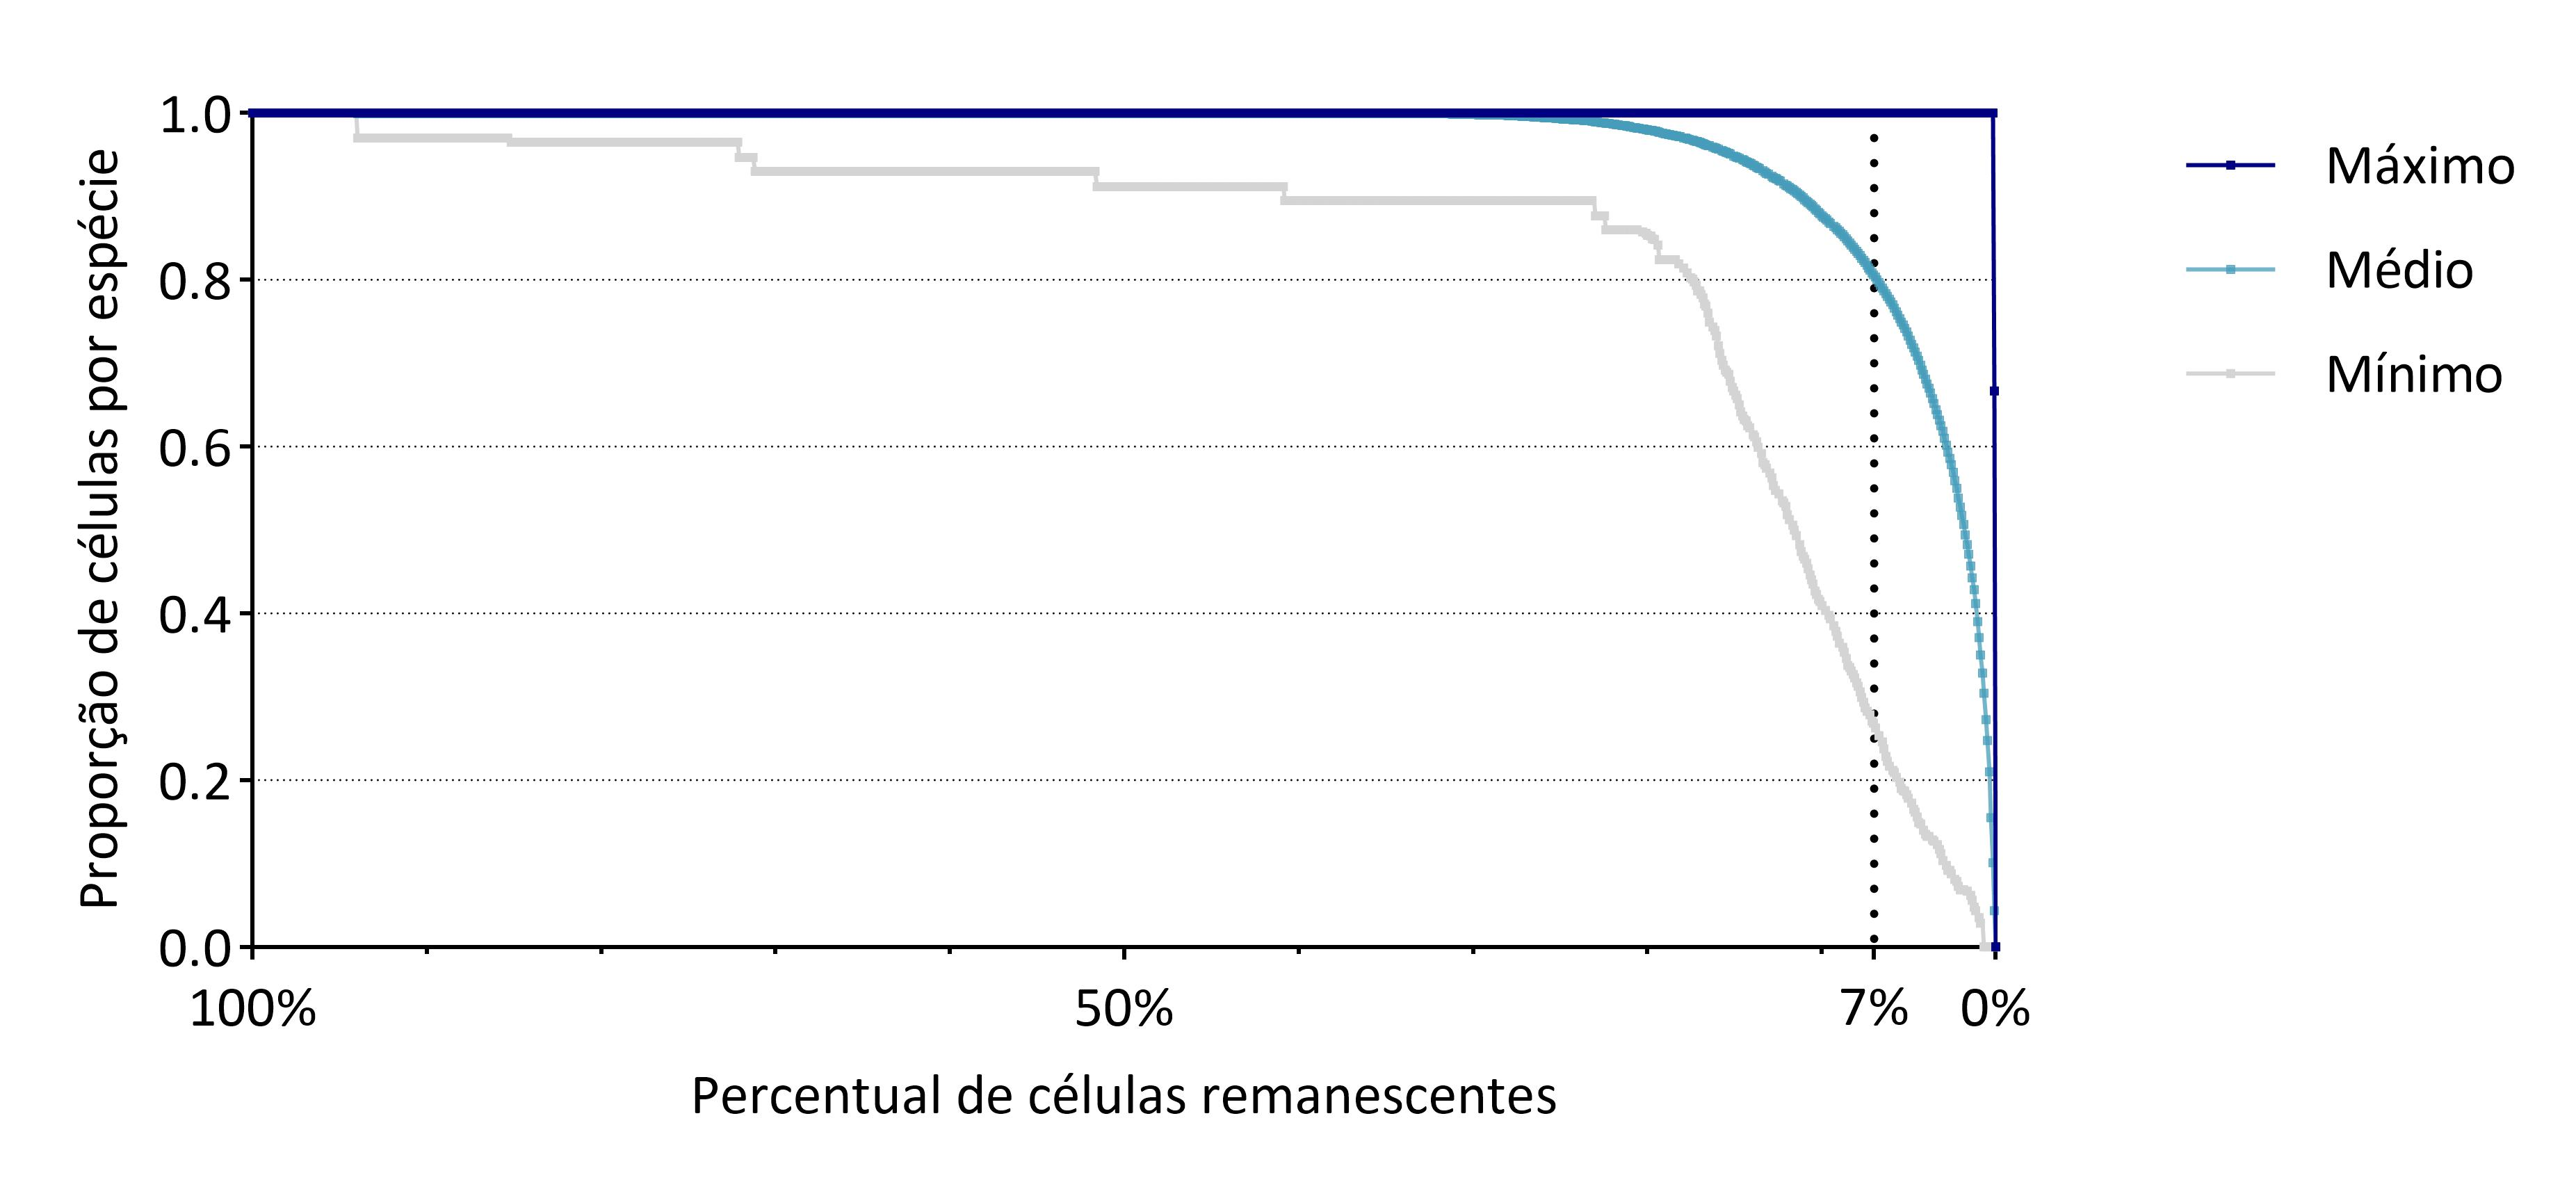
\includegraphics[width=0.85\linewidth]{imagens/cap07/Figura_7.1} 

}

\caption{Máximas, médias e mínimas das proporções totais de células por espécie de ave migratória conforme percentual de células totais remanescentes durante a priorização pelo Zonation e destaque do limiar de corte em 7\%.}\label{fig:21}
\end{figure}



Entre os padrões percebidos na solução por priorização por riqueza, ponderada pelos escores de vulnerabilidade para espécies de aves migratórias, está um adensamento das células recrutadas para a solução nas regiões Sul e Sudeste (Figura \ref{fig:30}). Tal fato decorre não só da relativa importância de áreas nessas regiões para as espécies de aves migratórias, mas também reflete um esforço de amostragem de aves em campo historicamente maior nessas duas regiões. Um segundo padrão que emerge é o recrutamento da maior parte do litoral brasileiro, justificado pela abundância de registros ao longo de toda rota Atlântica no país.

Com a meta de conservação adotada, das 16 espécies de aves migratórias nacionalmente ameaçadas, 14 tiveram 90\% ou mais das células com seus registros resguardadas na solução da priorização pelo Zonation (Tabela \ref{tab:tab04}).

\newpage

\begin{longtable}[t]{>{}l>{\centering\arraybackslash}p{4cm}>{\centering\arraybackslash}p{4cm}}
\caption{\label{tab:tab04}Percentual de células constantes na solução de priorização por riqueza, ponderada pelos escores de vulnerabilidade, para espécies de aves migratórias ameaçadas (conforme Portaria MMA nº 444/14).}\\
\toprule
Espécie & Categoria & \% de células na solução\\
\midrule
\em{Amazona pretrei} & VU & 70\\
\em{Sporophila melanogaster} & VU & 86\\
\em{Sporophila hypoxantha} & VU & 90\\
\em{Sporophila palustris} & VU & 91\\
\em{Stilpnia peruviana} & VU & 92\\
\addlinespace
\em{Calidris pusilla} & EN & 92\\
\em{Sterna hirundinacea} & VU & 94\\
\em{Limnodromus griseus} & CR & 95\\
\em{Thalasseus maximus} & EN & 98\\
\em{Calidris canutus} & CR & 99\\
\addlinespace
\em{Calidris subruficollis} & VU & 100\\
\em{Pterodroma arminjoniana} & CR & 100\\
\em{Puffinus lherminieri} & CR & 100\\
\em{Sporophila beltoni} & VU & 100\\
\em{Sporophila ruficollis} & VU & 100\\
\addlinespace
\em{Sterna dougallii} & VU & 100\\
\bottomrule
\end{longtable}

Do mesmo modo, a meta de conservação adotada também garantiu que, para as espécies menos comuns, ou seja, aquelas com registros em 20 células ou menos, 100\% das suas células estejam presentes na solução (Tabela \ref{tab:tab05}).

\newpage

\begin{ThreePartTable}
\begin{TableNotes}
\item[a] Com corte em 7\%, para as espécies de aves migratórias, ordenadas pelas espécies menos comuns.
\end{TableNotes}
\begin{longtable}[t]{>{}l>{\centering\arraybackslash}p{4cm}>{\centering\arraybackslash}p{4cm}}
\caption{\label{tab:tab05}Percentual de células com registros na solução de priorização pelo Zonation por espécie.}\\
\toprule
Espécie & Nº de células com registros pré priorização & \% de células com registro na solução\\
\midrule
\endfirsthead
\caption[]{\label{tab:tab05}Percentual de células com registros na solução de priorização pelo Zonation por espécie. \textit{(continuação)}}\\
\toprule
Espécie & Nº de células com registros pré priorização & \% de células com registro na solução\\
\midrule
\endhead

\endfoot
\bottomrule
\insertTableNotes
\endlastfoot
\em{Myiodynastes luteiventris} & 1 & 100\\
\em{Parkesia motacilla} & 1 & 100\\
\em{Progne cryptoleuca} & 1 & 100\\
\em{Progne dominicensis} & 1 & 100\\
\em{Spatula platalea} & 1 & 100\\
\addlinespace
\em{Chaetura pelagica} & 2 & 100\\
\em{Coccyzus erythropthalmus} & 2 & 100\\
\em{Icterus galbula} & 2 & 100\\
\em{Micrococcyx cinereus} & 2 & 100\\
\em{Puffinus lherminieri} & 2 & 100\\
\addlinespace
\em{Tringa inornata} & 2 & 100\\
\em{Mareca sibilatrix} & 3 & 100\\
\em{Asemospiza obscura} & 4 & 100\\
\em{Calidris mauri} & 4 & 100\\
\em{Sporophila iberaensis} & 4 & 100\\
\addlinespace
\em{Conothraupis speculigera} & 5 & 100\\
\em{Phaeomyias murina} & 5 & 100\\
\em{Pterodroma arminjoniana} & 5 & 100\\
\em{Vireo flavoviridis} & 6 & 100\\
\em{Nengetus coronatus} & 9 & 100\\
\addlinespace
\em{Chionis albus} & 12 & 100\\
\em{Empidonax alnorum} & 14 & 100\\
\em{Serpophaga munda} & 14 & 100\\
\em{Heteronetta atricapilla} & 15 & 100\\
\em{Phytotoma rutila} & 16 & 100\\
\addlinespace
\em{Catharus minimus} & 17 & 100\\
\em{Oreopholus ruficollis} & 18 & 100\\
\em{Chlidonias niger} & 19 & 100\\
\em{Cypseloides niger} & 19 & 100\\
\em{Onychoprion fuscatus} & 20 & 100\\
\addlinespace
\em{Setophaga ruticilla} & 22 & 96\\
\em{Chroicocephalus cirrocephalus} & 23 & 100\\
\em{Spatula discors} & 23 & 100\\
\em{Larus atlanticus} & 24 & 100\\
\em{Charadrius falklandicus} & 25 & 100\\
\addlinespace
\em{Sporophila ruficollis} & 27 & 100\\
\em{Progne elegans} & 28 & 100\\
\em{Oxyura vittata} & 32 & 97\\
\em{Calidris bairdii} & 33 & 100\\
\em{Anthus correndera} & 34 & 97\\
\addlinespace
\em{Phoenicopterus chilensis} & 35 & 100\\
\em{Dolichonyx oryzivorus} & 37 & 84\\
\em{Spatula versicolor} & 37 & 95\\
\em{Catharus swainsoni} & 37 & 100\\
\em{Serpophaga griseicapilla} & 39 & 97\\
\addlinespace
\em{Cinclodes fuscus} & 40 & 95\\
\em{Sporophila hypochroma} & 41 & 88\\
\em{Pseudocolopteryx acutipennis} & 41 & 95\\
\em{Vireo altiloquus} & 41 & 100\\
\em{Sterna dougallii} & 43 & 100\\
\addlinespace
\em{Piranga rubra} & 44 & 93\\
\em{Setophaga petechia} & 45 & 73\\
\em{Charadrius modestus} & 51 & 100\\
\em{Setophaga striata} & 53 & 79\\
\em{Inezia inornata} & 53 & 89\\
\addlinespace
\em{Ictinia mississippiensis} & 54 & 80\\
\em{Lessonia rufa} & 55 & 100\\
\em{Pheucticus aureoventris} & 57 & 56\\
\em{Tyrannus tyrannus} & 62 & 86\\
\em{Calidris subruficollis} & 62 & 100\\
\addlinespace
\em{Sporophila beltoni} & 63 & 100\\
\em{Vireo olivaceus} & 69 & 81\\
\em{Buteo swainsoni} & 69 & 88\\
\em{Sternula antillarum} & 71 & 97\\
\em{Contopus cooperi} & 78 & 81\\
\addlinespace
\em{Sterna paradisaea} & 84 & 92\\
\em{Leucophaeus atricilla} & 84 & 93\\
\em{Contopus virens} & 86 & 73\\
\em{Pseudocolopteryx flaviventris} & 87 & 94\\
\em{Riparia riparia} & 93 & 91\\
\addlinespace
\em{Sporophila palustris} & 93 & 91\\
\em{Buteo platypterus} & 94 & 79\\
\em{Gelochelidon nilotica} & 94 & 98\\
\em{Sterna trudeaui} & 99 & 98\\
\em{Phalaropus tricolor} & 102 & 96\\
\addlinespace
\em{Tachycineta leucopyga} & 103 & 93\\
\em{Calidris himantopus} & 104 & 97\\
\em{Polystictus pectoralis} & 107 & 86\\
\em{Coscoroba coscoroba} & 114 & 94\\
\em{Neochen jubata} & 119 & 56\\
\addlinespace
\em{Netta peposaca} & 124 & 84\\
\em{Limnodromus griseus} & 126 & 95\\
\em{Limosa haemastica} & 130 & 92\\
\em{Dacnis nigripes} & 139 & 87\\
\em{Sterna hirundinacea} & 141 & 94\\
\addlinespace
\em{Pygochelidon melanoleuca} & 144 & 64\\
\em{Sporophila cinnamomea} & 151 & 82\\
\em{Sporophila melanogaster} & 152 & 86\\
\em{Calidris canutus} & 154 & 99\\
\em{Chordeiles minor} & 156 & 81\\
\addlinespace
\em{Tringa semipalmata} & 160 & 98\\
\em{Stilpnia peruviana} & 169 & 92\\
\em{Thalasseus maximus} & 171 & 98\\
\em{Catharus fuscescens} & 179 & 53\\
\em{Sporophila hypoxantha} & 183 & 90\\
\addlinespace
\em{Calidris minutilla} & 187 & 84\\
\em{Nyctanassa violacea} & 193 & 95\\
\em{Hymenops perspicillatus} & 204 & 82\\
\em{Amazona pretrei} & 206 & 70\\
\em{Bartramia longicauda} & 213 & 78\\
\addlinespace
\em{Numenius hudsonicus} & 222 & 94\\
\em{Callonetta leucophrys} & 230 & 83\\
\em{Calidris pusilla} & 231 & 92\\
\em{Anas georgica} & 232 & 78\\
\em{Petrochelidon pyrrhonota} & 247 & 75\\
\addlinespace
\em{Attila phoenicurus} & 248 & 75\\
\em{Pluvialis squatarola} & 250 & 94\\
\em{Mimus triurus} & 251 & 80\\
\em{Thalasseus acuflavidus} & 252 & 95\\
\em{Progne subis} & 255 & 65\\
\addlinespace
\em{Pardirallus sanguinolentus} & 289 & 86\\
\em{Elaenia chilensis} & 296 & 65\\
\em{Arenaria interpres} & 296 & 92\\
\em{Sterna hirundo} & 301 & 91\\
\em{Calidris alba} & 301 & 94\\
\addlinespace
\em{Coccyzus americanus} & 303 & 74\\
\em{Dendrocygna bicolor} & 306 & 81\\
\em{Charadrius semipalmatus} & 405 & 88\\
\em{Lurocalis semitorquatus} & 421 & 74\\
\em{Pluvialis dominica} & 423 & 84\\
\addlinespace
\em{Calidris fuscicollis} & 448 & 85\\
\em{Calidris melanotos} & 450 & 83\\
\em{Plegadis chihi} & 465 & 74\\
\em{Sublegatus modestus} & 472 & 45\\
\em{Elaenia chiriquensis} & 477 & 55\\
\addlinespace
\em{Falco peregrinus} & 482 & 80\\
\em{Cyanoloxia glaucocaerulea} & 494 & 68\\
\em{Sporophila bouvreuil} & 500 & 56\\
\em{Casiornis fuscus} & 520 & 27\\
\em{Tringa melanoleuca} & 602 & 83\\
\addlinespace
\em{Turdus subalaris} & 615 & 68\\
\em{Harpagus diodon} & 616 & 74\\
\em{Turdus flavipes} & 622 & 65\\
\em{Hirundo rustica} & 625 & 68\\
\em{Griseotyrannus aurantioatrocristatus} & 655 & 50\\
\addlinespace
\em{Podager nacunda} & 687 & 74\\
\em{Rynchops niger} & 688 & 71\\
\em{Actitis macularius} & 693 & 74\\
\em{Elaenia parvirostris} & 720 & 74\\
\em{Fluvicola albiventer} & 729 & 48\\
\addlinespace
\em{Myiopagis viridicata} & 742 & 52\\
\em{Hydropsalis parvula} & 750 & 62\\
\em{Chaetura meridionalis} & 809 & 70\\
\em{Tringa flavipes} & 849 & 77\\
\em{Elaenia spectabilis} & 913 & 58\\
\addlinespace
\em{Tyrannus albogularis} & 926 & 45\\
\em{Legatus leucophaius} & 944 & 64\\
\em{Platalea ajaja} & 983 & 69\\
\em{Pandion haliaetus} & 1013 & 62\\
\em{Elanoides forficatus} & 1086 & 57\\
\addlinespace
\em{Coccyzus melacoryphus} & 1195 & 59\\
\em{Lathrotriccus euleri} & 1218 & 57\\
\em{Florisuga fusca} & 1234 & 54\\
\em{Pachyramphus validus} & 1301 & 55\\
\em{Myiarchus swainsoni} & 1359 & 57\\
\addlinespace
\em{Porphyrio martinica} & 1420 & 54\\
\em{Myiophobus fasciatus} & 1498 & 55\\
\em{Anthracothorax nigricollis} & 1504 & 53\\
\em{Tringa solitaria} & 1533 & 53\\
\em{Pachyramphus polychopterus} & 1551 & 56\\
\addlinespace
\em{Rostrhamus sociabilis} & 1588 & 54\\
\em{Sporophila lineola} & 1657 & 44\\
\em{Vireo chivi} & 1677 & 58\\
\em{Ictinia plumbea} & 1697 & 46\\
\em{Pyrocephalus rubinus} & 1821 & 51\\
\addlinespace
\em{Tersina viridis} & 1862 & 48\\
\em{Progne tapera} & 1965 & 55\\
\em{Turdus amaurochalinus} & 2103 & 49\\
\em{Sporophila caerulescens} & 2185 & 46\\
\em{Progne chalybea} & 2233 & 51\\
\addlinespace
\em{Empidonomus varius} & 2236 & 49\\
\em{Myiodynastes maculatus} & 2446 & 44\\
\em{Stelgidopteryx ruficollis} & 2495 & 45\\
\em{Tyrannus savana} & 2704 & 44\\
\em{Pitangus sulphuratus} & 3048 & 43\\
\addlinespace
\em{Tyrannus melancholicus} & 3250 & 40\\*
\end{longtable}
\end{ThreePartTable}

\hypertarget{abordagem-2-uxe1reas-de-agregauxe7uxe3o-de-indivuxedduos}{%
\section{Abordagem 2: Áreas de agregação de indivíduos}\label{abordagem-2-uxe1reas-de-agregauxe7uxe3o-de-indivuxedduos}}

Para a determinação das Áreas de Concentração pelo critério da expressiva agregação de indivíduos de espécies de aves migratórias ou parcialmente migratórias inicialmente foi realizado um levantamento bibliográfico em publicações científicas nacionais e estrangeiras. Porém, é possível que nem todas as áreas de expressiva agregação registradas na literatura tenham sido encontradas. Cientes dessa limitação, em 2021 foi realizada uma consulta \emph{on-line} direcionada à comunidade brasileira de ornitólogos cadastrada no Sistema de Autorização e Informação em Biodiversidade - SISBIO, no Sistema Nacional de Anilhamento - SNA e na Sociedade Brasileira de Ornitologia - SBO. Na ocasião, estes especialistas foram consultados sobre a validade das áreas de agregação constantes na 3ª edição do \emph{Relatório de Rotas e Áreas de Concentração de Aves Migratórias no Brasil}, bem como sobre a necessidade de inclusão de novas áreas com base em sua experiência de campo e/ou informações não publicadas. Por fim, as sugestões recebidas foram validadas pela equipe técnica do CEMAVE quanto ao atendimento aos critérios previamente estabelecidos. A participação da comunidade ornitológica é reconhecida ao final deste relatório, onde são nominados todos os que colaboraram.

A definição das áreas de concentração de aves migratórias pode não ser tarefa simples, uma vez que o próprio conceito de concentração pode ser variável. Influenciam nessa decisão parâmetros como tamanho da população global ou regional da espécie, socialidade habitual, objetivo da agregação e grau de risco de extinção da espécie (muitas vezes coincidente com o pequeno tamanho da população).

Para espécies com populações muito numerosas (como as andorinhas, por exemplo), uma agregação de uma centena de indivíduos pode não significar muito, mas algumas espécies com populações menores concentram uma grande porcentagem dos indivíduos em um único lugar, em algum período do ano, como ocorre com alguns \emph{Sporophila} mais raros, para os quais uma concentração de uma centena é considerada relevante.

Agregações de indivíduos de uma espécie que normalmente não são observados em bandos ou não se reúnem em números tão altos em suas atividades diárias alertam para uma situação peculiar, para a qual pode ser necessária proteção especial. O gavião-caramujeiro (\emph{Rostrhamus sociabilis}), por exemplo, é visto frequentemente em poleiros noturnos que reúnem 50-60 indivíduos, mas grupos de 2.000-3.000 indivíduos indicam concentrações fora do comum, em áreas que devem receber atenção especial.

Aves limícolas podem ser vistas em pequenos bandos em qualquer lugar da zona costeira, mas não são encontradas às centenas em lugares aleatórios, mas sim em pequenas porções de habitat que oferecem as condições ideais para obtenção de alimento. Essas áreas raras dentro de um tipo de ambiente que parece homogêneo (mas não é) são buscadas pelos indivíduos em migração que podem ter que se deslocar milhares de quilômetros entre um ponto de alimentação e outro. Sem esses pontos de parada, os indivíduos podem ser incapazes de completar seu ciclo anual de deslocamento e a raridade desses locais gera agregações de centenas a milhares de indivíduos, de uma ou várias espécies. Há que se considerar que os pontos de parada (diferentemente do destino final) não necessariamente concentrarão todos os indivíduos em viagem em um único momento, de modo que é compreensível que essas áreas de concentração agreguem menos indivíduos que as áreas de invernagem, não sendo necessariamente menos importantes que estas.

Em vista do que foi aqui exposto, conclui-se que a definição das áreas de concentração de aves migratórias não é matemática e não segue uma regra geral, mas deve considerar os parâmetros aqui citados, que são variáveis de acordo com a espécie ou grupo alvo.

As áreas de expressiva agregação validadas foram sobrepostas à mesma grade de células utilizada pelo método anterior, de modo a padronizar os dois métodos e delimitar com precisão a localização geográfica das Áreas de Concentração de Aves Migratórias no Brasil. Todas as células que continham as áreas de agregação foram marcadas como solução deste método. Devido ao fato de a grade ser a mesma, muitas células selecionadas na solução da priorização pelo Zonation podem ser coincidentes com aquelas indicadas na solução pelo critério de agregação.

\newpage

\hypertarget{resultados-1}{%
\subsection{Resultados}\label{resultados-1}}

Foram compiladas 57 áreas de agregação, distribuídas por 490 células da grade em 19 estados, além de ilhas oceânicas. As áreas serão descritas nessa seção com as justificativas para sua delimitação e respectivas fontes de informação. A maior parte são áreas de ocorrência de espécies migratórias limícolas e costeiro-oceânicas. Poucas são as áreas com agregação expressiva de indivíduos de espécies florestais ou campestres. Tal padrão decorre das características de agregação das espécies limícolas e costeiro-oceânicas e, talvez, das limitações de conhecimento e disponibilidade de dados sobre as demais espécies.

A seguir são apresentadas as áreas de agregação de indivíduos de aves migratórias por região e estado:

\textbf{\emph{Região Nordeste}}

\textbf{Alagoas}

\textbf{1 - Pontal do Peba e ilha do Cabeço}: o pontal do Peba na Área de Proteção Ambiental (APA) de Piaçabuçu em Alagoas e a ilha do Cabeço, em Sergipe (na divisa com Alagoas), guardam a foz do rio São Francisco. Para esta área já foram registradas 19 espécies de aves migratórias, 14 delas neárticas. Maçaricos, batuíras e trinta-réis utilizam a região durante suas migrações para pouso e alimentação. Cabral et al.~(2006a, 2006b) registraram mais de 200 indivíduos de \emph{Calidris alba} (média mensal de avistamento) e 100 de \emph{Charadrius semipalmatus}. Azevedo Jr \& Larrazábal (2011) observaram bandos de 300 indivíduos de \emph{Sterna hirundo}.

\textbf{Bahia}

\textbf{2 - Mangue Seco}: inserido na APA de Mangue Seco, é o primeiro local de agregação de \emph{Sterna dougallii} conhecido para o Brasil. Esta espécie, com outros integrantes da família Laridae, como \emph{S. hirundo}, formam concentrações de 10.000 indivíduos (Hays et al.~1997 e 1999, Lima et al.~2004, Lima \& Lima 2011).

\textbf{3 - Baía de Todos os Santos e Cacha-Prego}: assim como Mangue Seco, historicamente, a baía de Todos os Santos, com seus mangues e praias, abrigava as maiores concentrações de aves migratórias neárticas da Bahia (Morrison et al.~1989). A área possui diferentes sítios reconhecidos como importantes para aves migratórias, como a barra do Paraguaçu e Salinas da Margarida. Recentemente, para um trecho de 275 ha de área intermareal, foram observados mais de 60 indivíduos de \emph{Calidris pusilla}, cerca de 40 \emph{C. alba}, mais de 20 \emph{Arenaria interpres} e seis indivíduos de \emph{Tringa semipalmata} (Lunardi et al.~2012). A região de Cacha-Prego, em seu extremo sul, é área de invernada de \emph{Sterna dougallii}, com agregações na casa dos milhares. Os bancos de areia que ocorrem no local são vitais para que as aves possam descansar durante a invernada e se alimentar em águas próximas (Lima \& Lima 2011).

\textbf{4 - Baía de Camamu}: nesta baía os bancos de areia são utilizados também por \emph{Sterna dougallii} e \emph{S. hirundo}, formando concentrações de mais de 3.000 indivíduos (Hays et al.~1997 e 1999, Lima et al.~2004).

\textbf{5 - Barra Velha e ilha Coroa Vermelha}: no município de Caravelas, a barra Velha e a ilha Coroa Vermelha apresentaram registros de mais de 600 indivíduos de \emph{Thalasseus acuflavidus}, cerca de 60 \emph{Sterna dougallii}, 25 \emph{S. hirundo} e mais de 90 \emph{T. maximus} (C. Campolina, com. pess. 2021).

\textbf{6 - Corumbau}: localizada no município de Porto Seguro, a estimativa das populações do gênero \emph{Sterna} em Corumbau é de 3000 indivíduos. As espécies mais abundantes são \emph{Sterna hirundo}, seguida de \emph{S. dougallii} e \emph{Thalasseus a. eurygnathus}.

\textbf{7 - Ponta do Curral}: próxima ao morro de São Paulo, no município de Valença. Segundo Lima et al.~(2004), dados de recuperação de aves anilhadas apontam que a área é importante para a migração de \emph{Sterna dougallii} e outros representantes da família Laridae.

\textbf{Ceará}

\textbf{8 - Ilha Grande}: ilha com cerca de 3.000 ha, com os mangues mais preservados do Nordeste, localizada no complexo estuarino do rio Timonha, em Ubatuba. Agregação de ao menos 14 espécies de limícolas migratórias de origem neártica (Charadriidae e Scolopacidae). As contagens mensais, que chegaram a 1805 aves, reportaram um máximo de 732 indivíduos de \emph{Calidris pusilla}, 700 \emph{C. minutilla}, 261 \emph{Numenius hudsonicus}, 244 \emph{Arenaria interpres}, 196 \emph{Pluvialis squatarola} e 128 \emph{Charadrius semipalmatus} (Fedrizzi et al.~2016).

\textbf{9 - Região do Banco dos Cajuais}: o Banco dos Cajuais é uma área úmida costeira com mais de 70.000 ha, entre os estuários dos rios Jaguaribe e Apodi (RN), localizada parcialmente em algumas unidades de conservação: APA municipal de Canoa Quebrada, APA municipal da Praia de Ponta Grossa e APA municipal do Manguezal da Barra Grande. O local inclui extensas zonas intertidais, as maiores do estado, praias, restinga, mangues e um mosaico de salinas e lagoas usadas para extração de sal e cultivo de camarão. Em 2017, parte desta área foi reconhecida e como \href{http://whsrn.org/whsrn_sites/banco-dos-cajuais}{sítio da \emph{Western Hemisphere Shorebird Reserves Network} (WHSRN)} por concentrar aves limícolas migratórias, registrando cerca de 1\% das populações globais de \emph{Calidris canutus rufa} e de \emph{Limnodromus griseus griseus}. Outras 19 espécies migratórias neárticas são também registradas na área (Girão \& Albano 2011, Fedrizzi et al.~2016).

\textbf{Maranhão}

\textbf{10 - Reentrâncias Maranhenses}: área litorânea que se estende desde a foz do rio Gurupi, divisa com o estado do Pará a oeste, até a ilha do Cajual a leste, já limitando com o golfo do Maranhão. Distribui-se entre os biomas amazônico e marinho costeiro, estando parcialmente protegida pela Reserva Extrativista (RESEX) de Cururupu (Figura \ref{fig:22}) e pela APA das Reentrâncias Maranhenses. Desde 1991, é \href{http://whsrn.org/whsrn_sites/reentrancias-maranhenses}{reconhecida como de importância hemisférica para aves limícolas migratórias pela WHSRN}. Foi incluída na Convenção de Ramsar em 1993 (Serrano 2011) e, em composição com as Reentrâncias Paraenses, considerada uma IBA (Área Importante para a Conservação de Aves) (De Luca et al.~2009). Morrison et al.~(1989) destacam a área como a terceira maior em importância no continente para as aves limícolas neárticas e a mais importante do Brasil. Em termos de diversidade e abundância, as principais baías e localidades conhecidas das Reentrâncias Maranhenses utilizadas pelos migrantes neárticos são: Lençóis (ilhas de Maiaú, Campechá e salina de Iguará), Turiaçu (ilha da Croa dos Ovos e salina do Inglês) (Schulz-Neto \& Sousa 1995), croa Alta, ponta Seca, ilha de São Lucas, ponta de Muricitiuia, Mangunça, ponta da Croa, Porto Alegre, São João Mirim, Mangue Seco, Caçacueira e ilha do Cajual (Rodrigues \& Carvalho 2011a). Como exemplos de agregações temos a ilha do Cajual, com mais de 20.000 indivíduos de \emph{Calidris pusilla} e 3.600 de \emph{Limnodromus griseus} (Rodrigues 2000), a ponta Seca, em Cururupu, com 1.200 indivíduos de \emph{Limnodromus griseus} (Rodrigues 2007), a croa Alta, também em Cururupu, com 700 indivíduos de \emph{Pluvialis squatarola} (Rodrigues \& Carvalho 2011a) e mesmo número de \emph{Numenius hudsonicus} (Rodrigues 2007).

\begin{figure}[H]

{\centering 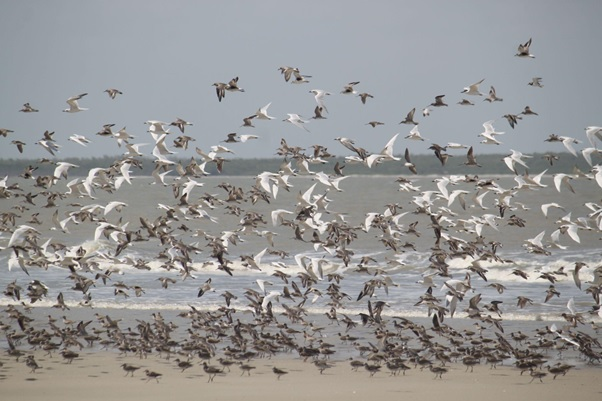
\includegraphics[width=0.75\linewidth]{imagens/cap07/Figura_7.2} 

}

\caption{Revoada de aves migratórias na Reserva Extrativista Cururupu. Foto: Danielle Paludo}\label{fig:22}
\end{figure}



\textbf{11 - Baixada Maranhense}: assim como a área anterior, é reconhecida como uma IBA e como um sítio Ramsar, sendo parcialmente protegida pela APA da Baixada Maranhense. Toda a área apresenta importantes sítios de alimentação e repouso para aves migratórias (Roth \& Scott 1987). Ao norte desta área, considerando ainda a ilha do Cajual, Rodrigues (2000) registrou quase 90.000 indivíduos de migratórias neárticas ao longo de um ano. Na ilha dos Caranguejos, observam-se picos de abundância entre os meses de setembro e fevereiro, com mais de 40.000 aves de 13 espécies neárticas (Carvalho \& Rodrigues 2011). Ao sul, mais de 20 espécies de maçaricos e batuíras foram observadas na região da baixada, concentrando-se em maior número nas proximidades de Viana, inclusive na bacia do rio Pindaré e na bacia do rio Mearim, sendo que cinco espécies se reproduzem na região. As mais abundantes em outubro de 1985 foram \emph{Calidris minutilla} e \emph{Charadrius semipalmatus}, observadas aos milhares na região de Viana. Mais para o interior observa-se as espécies \emph{Tringa melanoleuca} e \emph{T. flavipes}, \emph{Bartramia longicauda} e \emph{Pluvialis dominica} (Roth \& Scott 1987). A Baixada Maranhense também é um dos poucos lugares do Brasil onde há numerosas concentrações de \emph{Porphyrio martinica}, um ralídeo de hábito migratório (De Luca et al.~2009).

\textbf{12 - Praias de Raposo e Panaquatira}: na ilha de São Luís, destacam-se pela importância para aves migratórias as praias de Panaquatira, protegida pela APA Upaon-açu-Miritiba (Rodrigues \& Carvalho 2011a), onde censos mensais chegaram a registrar mais de 1.000 indivíduos de 10 espécies neárticas (Almeida \& Rodrigues 2015), e a do Raposo, na ilha de Curupu, onde Silva \& Rodrigues (2015) registraram 181 aves/ha, com destaque para \emph{Calidris pusilla}, \emph{Tringa semipalmata} e \emph{Pluvialis squatarola}. A ilha de Curupu abriga ainda importante colônia reprodutiva de \emph{Sternula antillarum} no Brasil (Rodrigues et al.~2010).

\textbf{Paraíba}

\textbf{13 - Ilha da Restinga}: um bando com cerca de 800 indivíduos de \emph{Charadrius semipalmatus} foi registrado no telhado de um galpão na margem da BR-230, nas proximidades da ilha da Restinga. Essa espécie utiliza a ilha como área de alimentação e repouso (Cardoso \& Zeppelini 2013). Outras espécies também são comumente observadas na região do estuário do rio Paraíba, como \emph{Pluvialis squatarola}, \emph{Numenius hudsonicus}, \emph{Tringa melanoleuca} e \emph{Calidris pusilla} (Cardoso \& Zeppelini 2011).

\textbf{Pernambuco}

\textbf{14 - Parque dos Manguezais}: nesta área de manguezal, inserida na malha urbana de Recife, censos registraram concentrações na ordem de 3.000 indivíduos de \emph{Calidris pusilla} (W. Telino-Jr, com. pess. 2021).

\textbf{15 - Ilha da Coroa do Avião}: ilhota situada no Canal de Santa Cruz e uma importante área para a migração de \emph{Calidris alba} (Lyra-Neves et al.~2004), com registros de mais de 400 indivíduos utilizando os bancos de areia da ilha (Cardoso \& Nascimento 2007).

\textbf{Rio Grande do Norte}

\textbf{16 - Foz do rio Apodi-Mossoró e salinas de Areia Branca}: área de alimentação e descanso para aves migratórias situada entre os municípios de Grossos e Areia Branca. Na foz do rio Apodi-Mossoró, em duas contagens de ponto fixo e uma embarcada, foram observados 787 indivíduos de 13 espécies limícolas migratórias. As maiores concentrações foram de \emph{Tringa melanoleuca}, com 522 indivíduos. Também destacaram-se espécies não limícolas, como \emph{Rynchops niger} (93) e \emph{Gelochelidon nilotica} (78) (Oliveira et al.~2015). Já nas salinas, em uma pequena área de 145 ha, foram realizados avistamentos de centenas de \emph{Charadrius semipalmatus}, \emph{Calidris canutus}, \emph{C. himantopus}, \emph{C. alba}, \emph{C. pusilla}, \emph{Limnodromus griseus} e \emph{Tringa flavipes} (Elias 2017).

\textbf{17 - Complexo Litorâneo da Bacia Potiguar}: abrange várias localidades importantes por concentrações de aves migratórias desde Macau (Figura \ref{fig:23}), a oeste, a Galinhos, a leste: as salinas de Macau e de Galinhos, salina Diamante Branco, a área em torno de Soledade e a lagoa Lagamar (Carnaubais e Porto de Mangue). Destacam-se os registros de grupos de mais de 1.000 indivíduos de \emph{Limnodromus griseus}, 2.800 \emph{Calidris pusilla} e mais de 400 indivíduos de \emph{Tringa flavipes} e \emph{Tringa melanoleuca} (Azevedo-Júnior \& Larrazábal 2011, Irusta \& Sagot-Martin 2011).

\begin{figure}[H]

{\centering 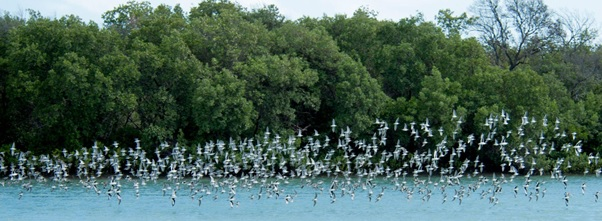
\includegraphics[width=0.75\linewidth]{imagens/cap07/Figura_7.3} 

}

\caption{Aves migratórias em Macau. Foto: João Damasceno}\label{fig:23}
\end{figure}

\textbf{18 - Lagoa de Guaraíras}: localizada no município de Tibau do Sul, as contagens realizadas em 2015 a partir de um transecto embarcado de 3,75 km de extensão registraram 4.306 indivíduos de 15 espécies, destacando-se \emph{Calidris pusilla} (3.297), \emph{Charadrius semipalmatus} (662), \emph{Arenaria interpres} (96), \emph{Limnodromus griseus} (93) e \emph{Calidris alba} (57). Em virtude da dificuldade de acesso às áreas lamacentas onde as aves concentravam-se durante a maré baixa, muitos indivíduos deixaram de ser contados (Oliveira et al.~2015).

\textbf{19 - Foz do rio Cunhaú}: situada no município de Canguaretama, 190 indivíduos de oito espécies migratórias neárticas foram observados em um trecho de 500 m de extensão, com destaque para \emph{Calidris pusilla} (107 ) e \emph{Charadrius semipalmatus} (47) (Oliveira et al.~2015).

\textbf{Sergipe}

\textbf{20 - Estuário do rio Sergipe e praia de Atalaia}: com registro de 12 espécies das famílias Charadriidae e Scolopacidae, o estuário do rio Sergipe apresentou registros de agregação de cerca de 2.200 indivíduos de \emph{Charadrius semipalmatus} e 200 de \emph{Numenius hudsonicus}. Na região também há registro de \emph{Falco peregrinus} e de \emph{Sterna hirundo}, com bandos de até 100 indivíduos acompanhando barcos de pesca (Sousa 2011a). Já na praia de Atalaia, ainda em Aracaju, foram observadas concentrações de 1.038 indivíduos de \emph{C. semipalmatus}, 1.075 de \emph{Calidris pusilla} e de até 400 de \emph{Calidris alba} (Almeida 2010, Almeida \& Ferrari 2011).

\textbf{21 - Praias e manguezais do estuário do rio Vaza-Barris}: espécies migratórias utilizam a área para alimentação e descanso durante a sua passagem pelo litoral brasileiro. As aves migratórias observadas no local foram \emph{Pandion haliaetus}, \emph{Pluvialis squatarola}, \emph{Charadrius semipalmatus}, \emph{Limnodromus griseus}, \emph{Numenius hudsonicus}, \emph{Actitis macularius}, \emph{Tringa solitaria}, \emph{Tringa melanoleuca}, \emph{Tringa flavipes}, \emph{Arenaria interpres}, \emph{Calidris canutus}, \emph{Calidris alba}, \emph{Calidris pusilla}, \emph{Sterna hirundo} e \emph{Sterna dougallii} (Schulz-Neto 1992 in: Sousa 2011b, Sousa et al.~2004). Essas espécies costumam descansar nos bancos de areia e forrageiam principalmente ao longo de praias e nestes bancos, como a crôa da Goré. Também forrageiam em bancos de lodo do rio Santa Maria e nas margens do rio Vaza-Barris e seus afluentes. Já em 1992, Schulz-Neto indicava a área do estuário do rio Vaza-Barris como ``importante para o descanso e alimentação de aves migratórias''. Em seu estudo foram observados 33 indivíduos de \emph{Charadrius semipalmatus}, 277 \emph{Calidris alba}, sete \emph{Numenius hudsonicus}, 54 \emph{Limnodromus griseus} e 68 \emph{Calidris pusilla}. \emph{Sterna hirundo} foi registrada no estuário, acompanhando barcos de pesca, em bandos de até 300 indivíduos (Sousa 2011b).

\textbf{22 - Complexo estuarino dos rios Piauí, Fundo e Real}: na divisa dos estados de Sergipe e Bahia, está incluído nos limites da Área de Proteção Ambiental do Litoral Sul do estado de Sergipe e é contíguo com a área de agregação de migratórias Mangue Seco, no estado da Bahia. Quinze espécies migratórias neárticas utilizam a área para repouso e/ou alimentação. Em 2007, foram observados mais de 300 indivíduos de \emph{Numenius hudsonicus} sobrevoando o estuário e alimentando-se nas margens do rio Real, próximo ao povoado Pontal, município de Indiaroba. Assim como para o estuário e foz do rio Vaza-Barris, Schulz-Neto \& Souza (1993) apontam a foz do rio Real, incluindo todo o complexo estuarino, como ``área importante para o descanso e alimentação das aves migratórias provenientes, em sua grande maioria, da região neártica'' (Sousa 2011c).

\textbf{\emph{Região Norte}}

\textbf{Amapá}

\textbf{23 - Praia do Goiabal}: historicamente conhecida como uma das áreas com maiores concentrações de migratórias neárticas no estado do Amapá (Morrison et. al.~1989). A praia do Goiabal apresentou a maior agregação de \emph{Calidris alba} na costa amazônica brasileira, com 3.000 indivíduos. Foi registrada também alta abundância de \emph{Calidris pusilla} (2400) e de \emph{Charadrius semipalmatus} (1.000), além de alguns indivíduos de \emph{Pluvialis squatarola}, \emph{Arenaria interpres}, \emph{Calidris canutus} e \emph{Tringa melanoleuca} (Rodrigues \& Carvalho 2011b), abundâncias que vêm sendo confirmadas em sobrevoos recentes (D. Paludo, com. pess. 2021).

\textbf{24 - Praias do Parque Nacional do Cabo Orange}: a área do Parque Nacional (PARNA) registra agregações de 10.000 indivíduos de \emph{Calidris pusilla} (Figura \ref{fig:24}), além de outras 17 espécies migratórias: \emph{Phoenicopterus ruber}, \emph{Platalea ajaja}, \emph{Pandion haliaetus}, \emph{Pluvialis squatarola}, \emph{Charadrius semipalmatus}, \emph{Numenius hudsonicus}, \emph{Actitis macularius}, \emph{Tringa solitaria}, \emph{T. melanoleuca}, \emph{T. semipalmata}, \emph{T. flavipes}, \emph{Arenaria interpres}, \emph{Calidris canutus}, \emph{C. alba}, \emph{C. pusilla}, \emph{Sterna hirundo} e \emph{Rynchops niger} (P. Silvestre \& D. Paludo, com. pess. 2021).

\begin{figure}[H]

{\centering 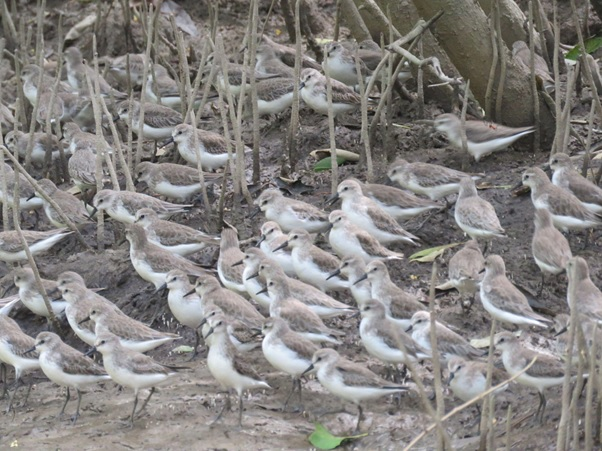
\includegraphics[width=0.75\linewidth]{imagens/cap07/Figura_7.4} 

}

\caption{\emph{Calidris pusilla} no Parna de Cabo Orange. Foto: Arquivo CEMAVE}\label{fig:24}
\end{figure}



\textbf{Amazonas}

\textbf{25 - Lagos e igarapés da Reserva Extrativista Catuá-Ipixuna}: \emph{Calidris melanotos} é a espécie com mais registros na área, com 63 indivíduos observados em um dos lagos. Cinquenta indivíduos de \emph{Calidris fuscicollis} foram registrados forrageando em outro lago. Na desembocadura do igarapé Catuá foi avistada uma dezena de \emph{Actitis macularius}, espécie eventualmente também observada em algumas praias do rio Solimões. Ao longo deste rio, entre os igarapés Catuá e Ipixuna, foram registrados vários indivíduos de \emph{Pandion haliaetus} e \emph{Tringa solitaria}. \emph{Tringa flavipes} foi encontrada na desembocadura do igarapé Catuá e há um avistamento de \emph{Pluvialis squatarola}. Avistamentos de \emph{Hirundo rustica} e \emph{Progne subis} são comuns. Vários indivíduos de \emph{H. rustica} foram avistados voando ao longo do rio Solimões, entre os igarapés Catuá e Ipixuna e, esporadicamente, em alguns lagos destes igarapés. Para \emph{P. subis} foi registrado um número máximo de cerca de 50 indivíduos (Andretti \& Costa 2011).

\textbf{26 - Lagos e igarapés da Reserva de Desenvolvimento Sustentável Piagaçu-Purus}: há registros de 13 espécies migrantes neárticas e a área é sítio reprodutivo de \emph{Rynchops niger}, em especial ao longo dos lagos, paranãs e igarapés ao redor do lago Ayapuá (Cintra et al.~2011).

\textbf{27 - Rio Solimões e afluentes na Reserva de Desenvolvimento Sustentável Mamirauá}: há registros de 25 espécies migrantes neárticas e a área é sítio reprodutivo de \emph{Rynchops niger} (Melo et al.~2011).

\textbf{28 - Ilhas do Cumaru e do Papagaio}: no baixo rio Negro, município de Iranduba, essas duas ilhotas apresentaram concentrações de mais de 250.000 indivíduos de andorinhas migratórias, principalmente \emph{Progne subis}, quando se reúnem para dormir. \emph{Progne tapera} também é abundante, mas sem estimativa populacional. As andorinhas estão presentes de janeiro a maio há pelo menos 15 anos consecutivos. Outras espécies migratórias na área são \emph{Pandion haliaetus}, \emph{Falco peregrinus}, \emph{Tyrannus savana} e \emph{Hirundo rustica} (M. Cohn-Haft, com. pess. 2021).

\textbf{Pará}

\textbf{29 - Reentrâncias Paraenses}: área litorânea que se estende desde a foz do rio Gurupi, divisa com o estado do Maranhão a leste, até a baía do Marajó. Distribui-se entre os biomas amazônico e marinho costeiro, estando parcialmente protegida por diversas reservas extrativistas, tendo sido incluída na Convenção de Ramsar em 2018 (área denominada Estuário do rio Amazonas e seus manguezais) e, junto com as Reentrâncias Maranhenses, é considerada uma IBA (Área Importante para a Conservação de Aves) (De Luca et al.~2009). Morrison et al.~(1989) destacam a área como uma das mais importantes no continente para as aves limícolas neárticas. Concentrações importantes de \emph{Calidris pusilla}, \emph{Leucophaeus atricilla}, \emph{Calidris canutus} e \emph{Pluvialis squatarola} foram verificadas na área, com máximos de 6.000, 3.000, 2.000 e 1.200 indivíduos, respectivamente. Observa-se, também, uma alta abundância de outros táxons migratórios, como \emph{Calidris alba} e \emph{Charadrius semipalmatus} (400 indivíduos), \emph{Arenaria interpres}, \emph{Numenius hudsonicus} e \emph{Limnodromus griseus} (todos com cerca de 300 indivíduos), e ainda avistamentos de cerca de 250 \emph{Thalasseus acuflavidus} e de 50 \emph{Actitis macularius} (Rodrigues \& Carvalho 2011c).

\textbf{Tocantins}

\textbf{30 - Parque Estadual do Cantão}: além de algumas espécies migratórias de Charadriiformes, foi registrado um bando de \emph{Progne subis} estimado em 5.000 a 8.000 indivíduos (Pinheiro \& Dornas 2009). Essa espécie de andorinha parece ser fiel ao sítio de invernada, sendo observada em anos consecutivos na região (Dornas \& Pinheiro 2011), que também é área de reprodução de \emph{Neochen jubata} (M. O. Barbosa, com. pess. 2021).

\textbf{\emph{Região Sudeste}}

\textbf{Espírito Santo}

\textbf{31 - Ilhas dos municípios de Vila Velha, Guarapari e Marataízes}: as ilhas Itatiaia, Escalvada (Figura \ref{fig:25}) e Branca abrigam as maiores colônias reprodutivas de \emph{Thalasseus acuflavidus} no Atlântico Sul, correspondendo a mais de 1\% da população global da espécie. Foram estimados 10.000 indivíduos na ilha Branca e de 10.000 a 13.000 indivíduos na ilha Escalvada (Efe et al.~2000). Ocorrem também colônias de \emph{Sterna hirundinacea} (Efe 2004). Nas ilhas Itatiaia há registros históricos de nidificação de \emph{Puffinus lherminieri} (Bencke et al.~2006).

\begin{figure}[H]

{\centering 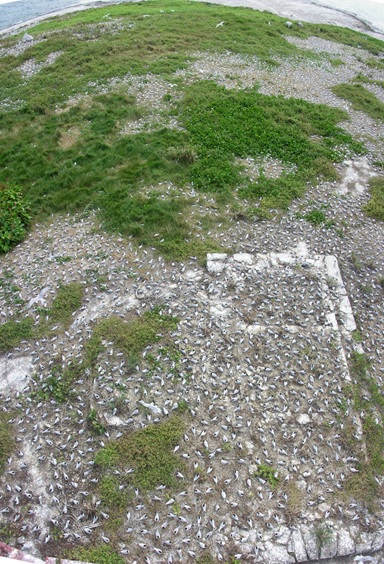
\includegraphics[width=0.4\linewidth]{imagens/cap07/Figura_7.5} 

}

\caption{Colônia reprodutiva de \emph{Thalasseus acuflavidus} na Ilha Escalvada. Foto: César Musso}\label{fig:25}
\end{figure}



\textbf{32 - Foz do rio Doce}: monitoramentos realizados na foz do rio Doce, decorrentes do rompimento da barragem de Fundão, apontaram 14 espécies migratórias neárticas entre outras espécies migratórias oceânicas, com contagens anuais totais de indivíduos chegando a 3.773 para \emph{Sterna hirundo} e 3.321 para \emph{Thalasseus acuflavidus}, além de avistamentos de 1.839 indivíduos de Sterninae por monitoramento com drone (Bianchini et al.~2020).

\textbf{Rio de Janeiro}

\textbf{33 - Região de Quissamã}: inclui o Parque Nacional da Restinga de Jurubatiba e destaca-se por abrigar grandes concentrações (mais de 6.000 indivíduos) de aves limícolas representadas principalmente por \emph{Calidris fuscicollis}, \emph{Calidris alba} e \emph{Tringa flavipes} (Tavares et al.~2015).

\textbf{São Paulo}

\textbf{34 - Várzea e foz do rio Embu-Mirim}: compreende as Áreas de Preservação Permanente (APP) das bacias dos rios Embu-Mirim e Guarapiranga. Foram registrados grupos de até 300 indivíduos de \emph{Tringa melanoleuca} e de até 200 de \emph{Tringa flavipes} (Schunck 2011).

\textbf{35 - Manguezais da baixada Santista}: circundados por três IBAs (SP04, SP05 e SP07) (Bencke et al.~2006), ainda que não contemplados por elas, os ecossistemas de mangues entre Cubatão, Praia Grande e a região da barra do canal de Bertioga ou manguezais da baixada Santista são formados por um complexo de ambientes transicionais. Tal diversidade reflete-se no número de espécies migratórias lá observadas: apenas dentre as migrantes neárticas há 17 táxons registrados, mas também ocorrem espécies com outros padrões de deslocamento. Citam-se, como exemplos: \emph{Dendrocygna bicolor}, \emph{Anas versicolor}, \emph{Platalea ajaja}, \emph{Nyctanassa violacea}, \emph{Porphyrio martinica}, \emph{Actitis macularius}, \emph{Calidris canutus}, \emph{C. pusilla}, \emph{Sterna hirundo}, \emph{S. hirundinacea}, \emph{Thalasseus maximus}, \emph{Tringa flavipes}, \emph{T. melanoleuca}, \emph{Charadrius semipalmatus}, \emph{Rynchops niger}, \emph{Pandion haliaetus}, \emph{Progne subis}, \emph{Hirundo rustica} e \emph{Coccyzus melacoryphus}. As espécies \emph{Platalea ajaja}, \emph{T. flavipes}, \emph{T. melanoleuca}, \emph{C. semipalmatus}, \emph{R. niger} e \emph{P. haliaetus} foram incluídas entre as espécies dominantes ou mais importantes para a comunidade de aves local. De outubro a novembro quase 1.000 indivíduos de \emph{T. flavipes} e de \emph{C. semipalmatus} chegam a ser observados na área, sendo esta também uma das mais importantes áreas de reprodução para \emph{N. violacea} na região Sudeste do Brasil, que forma colônias nos municípios de Cubatão, Santos e São Vicente (Olmos \& Silva e Silva 2001). Para a área também é reportado o avistamento de uma centena de \emph{P. ajaja} (D. N. Donadio, com. pess. 2021).

\textbf{36 - Arquipélago de Alcatrazes e ilhas costeiras do litoral paulista}: o arquipélago de Alcatrazes e a Ilha Bela, reconhecidos como IBA, bem como as ilhas costeiras de Castilho, as Lajes de Santos e da Conceição e o ilhote das Gaivotas são importantes áreas de reprodução para espécies marinhas e migratórias, especificamente para \emph{Sterna hirundinacea}, em sete áreas, e \emph{Thalasseus maximus}, em cinco áreas (Campos et al.~2004, Bencke et al.~2006). Para a Laje de Santos, que também é um parque estadual marinho, há observações de agregação e reprodução de \emph{Thalasseus acuflavidus} (Campos et al.~2004, Fey et al.~2017).

\textbf{\emph{Região Centro-Oeste}}

\textbf{Mato Grosso}

\textbf{37 - Chapada dos Guimarães}: área de ocorrência das espécies migratórias \emph{Ictinia mississippiensis} e \emph{Rostrhamus sociabilis} (Figura \ref{fig:26}), sendo que esse último foi observado em grupos de mais de 2.500 indivíduos (P. P. Amaral, com. pess. 2010).

\begin{figure}[H]

{\centering 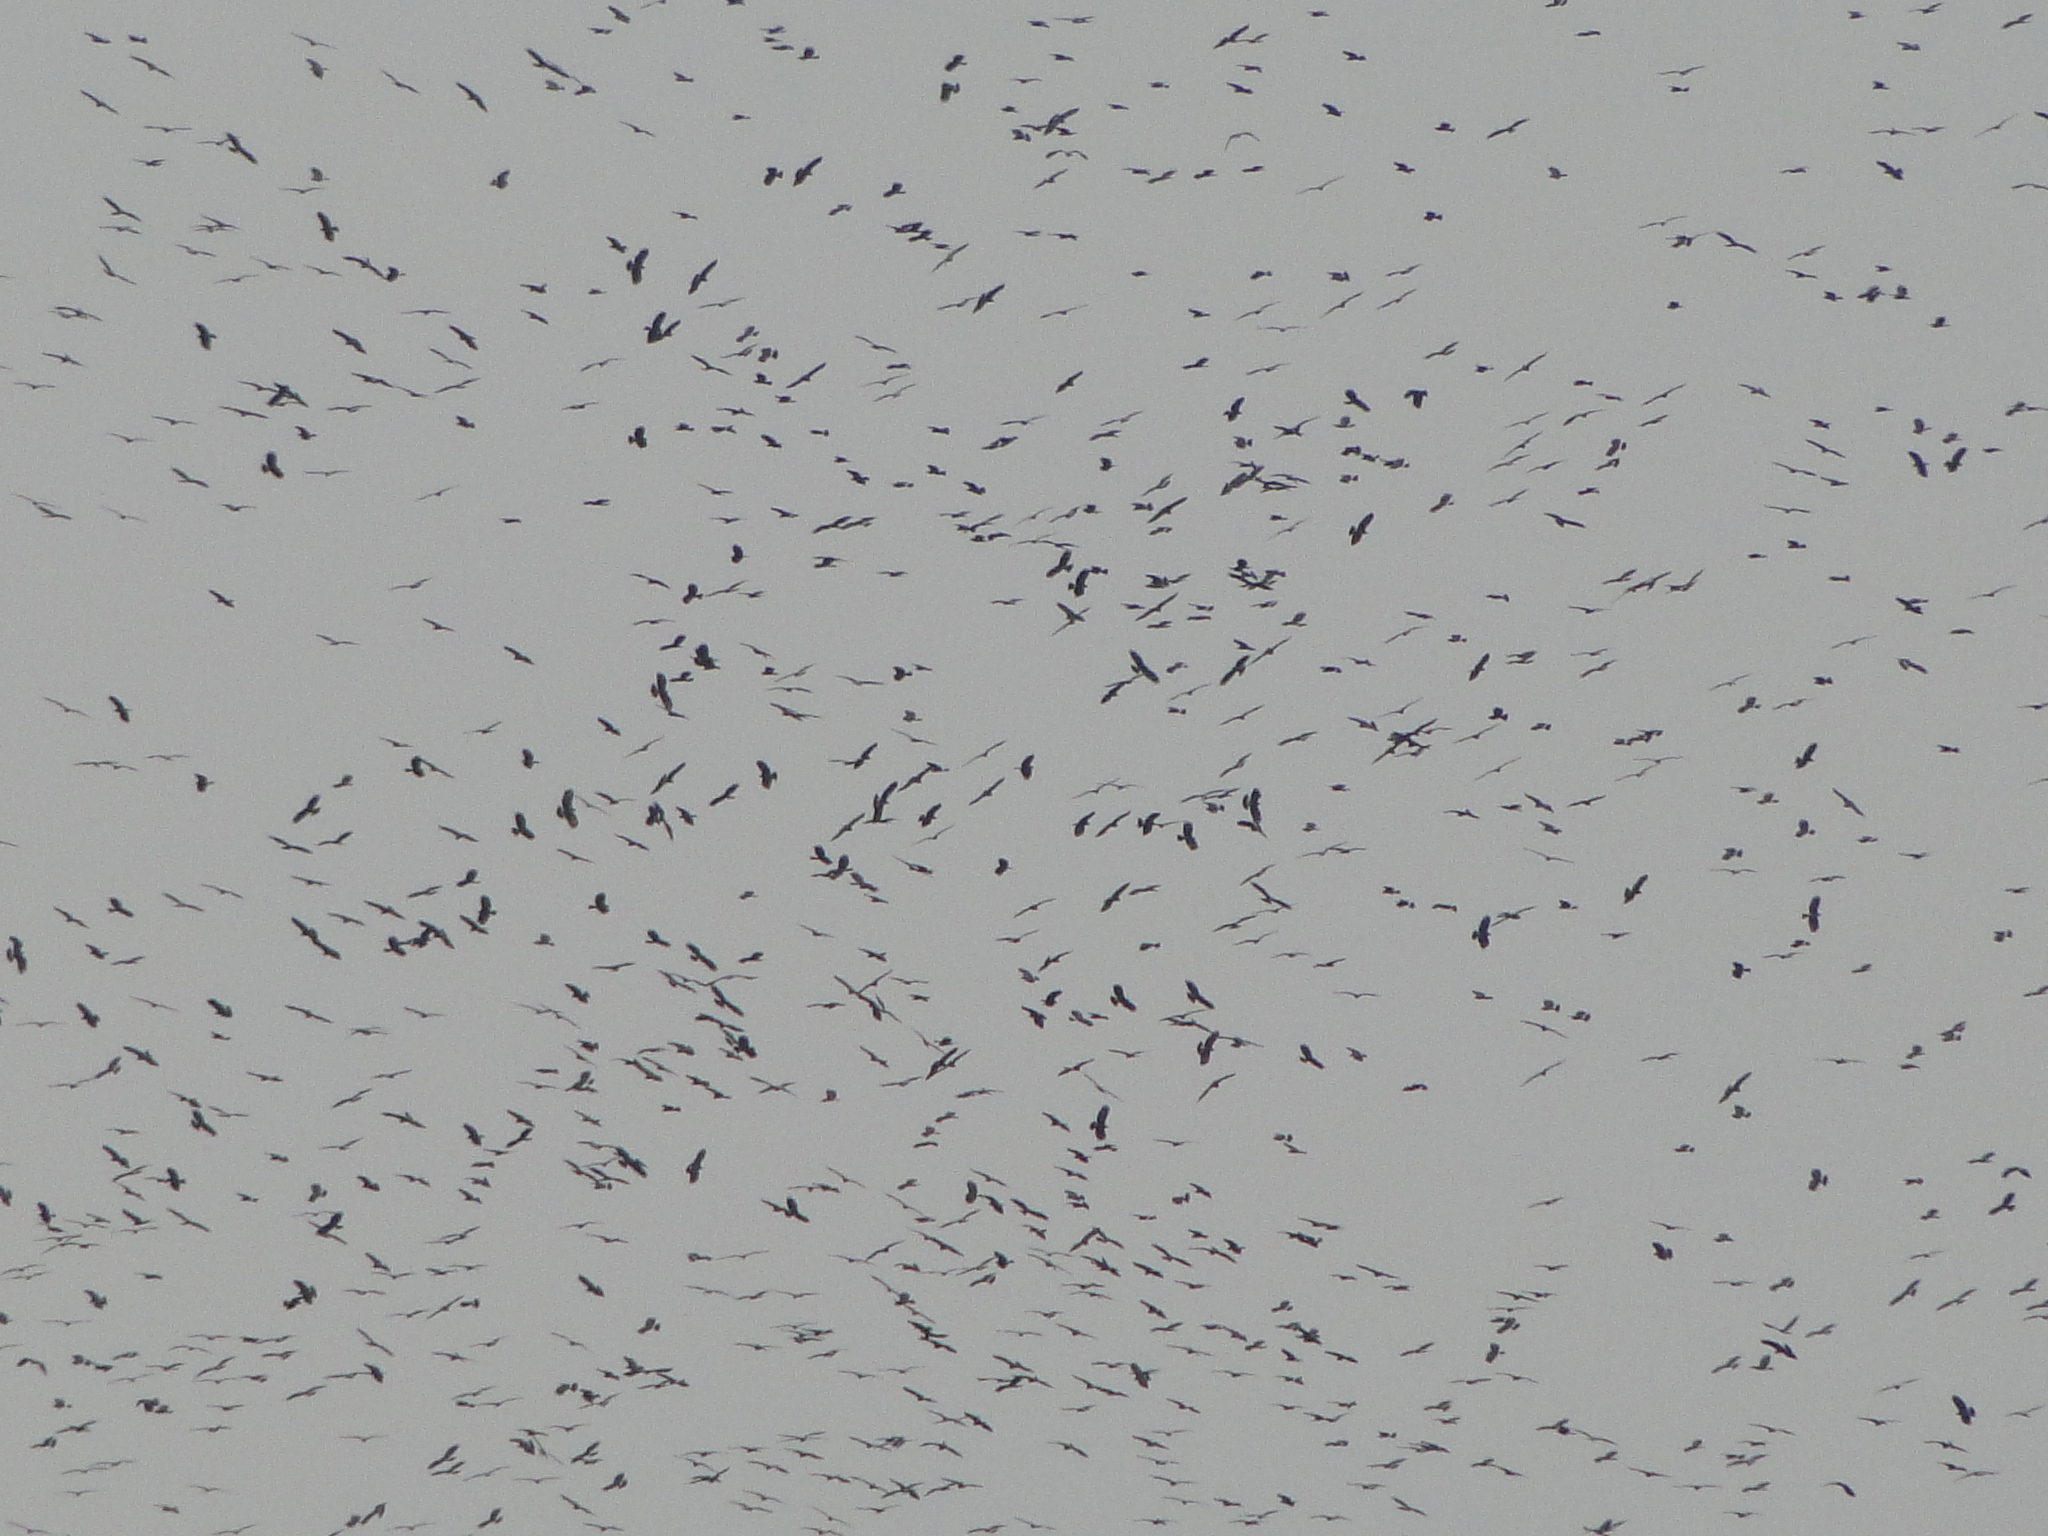
\includegraphics[width=0.75\linewidth]{imagens/cap07/Figura_7.6} 

}

\caption{Concentração de \emph{Rostrhamus sociabilis} (gavião-caramujeiro) na Chapada dos Guimarães. Foto: Mauricio Santos}\label{fig:26}
\end{figure}



\textbf{38 - Rio Cuiabá-Sesc Pantanal}: área reprodutiva de \emph{Rynchops niger}, com quantitativos de quase 600 indivíduos (Antas et al.~2016).

\textbf{39 - Estação Ecológica Taiamã e região}: para a unidade e região ao sul, são registrados sítios de dormitório e de alimentação ou invernada para as seguintes espécies migratórias: \emph{Rostrhamus sociabilis}, com estimativas de 1.500 a 2.000 indivíduos, \emph{Calidris fuscicollis}, concentrações de cerca de 150 indivíduos, \emph{Hirundo rustica}, cerca de 2.000 indivíduos, que podem ser observados em companhia de \emph{Petrochelidon pyrrhonota}, cerca de 3.000 indivíduos e, por fim, \emph{Rynchops niger}, que nidifica nas praias, com colônias estimadas em 1.000 indivíduos (A. V. B. Frota \& B. D. Vitorino, com. pess. 2021).

\textbf{\emph{Região Sul}}

\textbf{Paraná}

\textbf{40 - Parque Municipal Barigui}: foi registrado um número expressivo de \emph{Tringa flavipes} em 2006, quase 500 indivíduos (Deconto \& Aurelio-Silva 2011), assim como outras espécies migratórias, porém com poucos registros.

\textbf{41 - Parque Regional do Iguaçu e adjacências}: na área foram registrados 265 indivíduos de \emph{Tringa flavipes}, além de 49 de \emph{C. melanotos} e de 30 a 35 indivíduos de \emph{T. melanoleuca} (Vallejos et al.~2011).

\textbf{42 - Parque Nacional Marinho das Ilhas dos Currais, ilha da Figueira e ilhas Itacolomis}: são ilhas costeiras importantes como área de pouso e de reprodução das espécies migratórias \emph{Sterna hirundinacea} (100 casais) e \emph{Thalasseus acuflavidus} (100 casais) (Krul 2004). A área também é reconhecida como IBA (BR209) (Bencke et al.~2006).

\textbf{43 - Nordeste dos Campos Gerais}: área utilizada por uma população de \emph{Petrochelidon pyrrhonota} estimada em 1.500 a 2.000 indivíduos durante a invernada de 2007 (Santos 2011).

\textbf{44 - Trecho inferior do rio Ivaí}: esta área, que se distribui ao norte do rio Ivaí, entre sua foz e a localidade de Nordestina, em Amaporã, originalmente composta por várzeas, foi convertida em sua maior parte em lavouras de arroz. Contudo, ainda concentra grande riqueza de espécies migratórias, algumas delas formando grandes concentrações. Destacam-se \emph{Plegadis chihi}, com concentrações superiores a 4.000 indivíduos, \emph{Anas versicolor}, com cerca de 300 indivíduos, \emph{Platalea ajaja}, com cerca de 124 indivíduos, \emph{Rostrhamus sociabilis}, com contagens de até 78 indivíduos e \emph{Tringa flavipes}, com mais de 1.200 indivíduos (P. Scherer-Neto, A. Urben-Filho, A. Silva Júnior \& J. N. Campanha, com. pess. 2021).

\textbf{Rio Grande do Sul}

\textbf{45 - Banhado do Maçarico}: área categorizada como Refúgio de Vida Silvestre, o banhado do Maçarico também está incluído em uma área reconhecida como IBA (RS11). Nessa área foi registrada a maior população reprodutiva de \emph{Sporophila palustris} do Brasil (200 a 300 indivíduos -- cerca de 10\% da população global estimada), espécie migratória e ameaçada (Maurício et al.~2014) e há, ainda, registros de até 2800 indivíduos de \emph{Plegadis chihi} (Ebird- Banhado do Maçarico, 2022).

\textbf{46 - Estuário da laguna dos Patos}: localizado nos municípios de Rio Grande, Pelotas e São José do Norte, compreende o setor meridional da Lagoa dos Patos, entre a Ponta dos Lençóis a leste, a Lagoa Pequena a oeste e a barra do Canal de Rio Grande a sul, incluindo as ilhas da Torotama, do Leonídio, dos Marinheiros e ilhotas associadas, incluindo a APA municipal da Lagoa Verde, Eco-Museu da Ilha da Pólvora e RVS do Molhe Leste. Existem registros de 22 espécies de migrantes neárticos para este estuário. A região é importante sítio de estadia para \emph{Pluvialis dominica}, \emph{Tringa flavipes}, \emph{Calidris subruficollis}, \emph{Calidris fuscicollis}, \emph{Calidris melanotos}, \emph{Sterna hirundo} e \emph{Hirundo rustica}. Na ilha da Torotama, ao menos 545 indivíduos de \emph{P. dominica} e 800 indivíduos \emph{C. subruficollis} foram contados. Quando levemente inundados, os campos também são importantes para \emph{C. fuscicollis}, com pelo menos 688 indivíduos registrados no local. Aproximadamente 400 indivíduos de \emph{T. flavipes}, 100 \emph{C. fuscicollis}, 200 \emph{C. melanotos} e 500 \emph{H. rustica} foram observados na transição entre banhados de água doce e marismas na ilha da Torotama e banhado do Silveira (Dias et al.~2011). \emph{Calidris fuscicollis} é também frequente em praias arenosas e bordas de marismas do canal de Rio Grande, especialmente na localidade de Pontal Sul e arredores, onde até 500 indivíduos foram registrados (Vooren 1995). Esta localidade também é sítio de agregação de \emph{S. hirundo}. Totais de 3.725 e 5.580 indivíduos dessa espécie foram contados no Pontal Sul (Bugoni e Vooren 2005). Áreas planas areno-lamosas junto a marismas em sacos protegidos constituem sítio de forrageio e descanso para \emph{Pluvialis squatarola}, \emph{Charadrius semipalmatus}, \emph{Limosa haemastica}, \emph{Numenius hudsonicus}, \emph{T. flavipes}, \emph{Tringa melanoleuca}, \emph{Arenaria interpres} e \emph{Calidris canutus} (Resende \& Leeuwenberg 1987, Vooren 1995, Dias \& Maurício 1998, Dias et al.~2011), embora valores máximos de contagens dessas espécies não superem 100 indivíduos.

\textbf{47 - Reserva Biológica do Mato Grande e extremo sul do canal São Gonçalo}: em 2009 foram observadas nessas áreas concentrações de \emph{Plegadis chihi} de até 8.795 indivíduos (Vizentin-Bugoni et al.~2015). Há, ainda, registros expressivos de outras espécies migratórias: 384 indivíduos de \emph{Netta peposaca}, 270 \emph{Calidris melanotos}, 183 \emph{Coscoroba coscoroba}, 134 \emph{Rostrhamus sociabilis}, 80 \emph{Calidris fuscicollis}, 45 \emph{Tachycineta leucopyga} (Ebird - Estrada de Santa Izabel BR 473, 2022). Também são áreas de reprodução de \emph{Sporophila palustris}, que além de migratória, é uma espécie ameaçada (Maurício et al.~2014).

\textbf{48 - Banhado do Taim}: reconhecido como IBA (RS12) (Bencke et al.~2006) e sítio Ramsar, o banhado do Taim está contemplado em parte pela Estação Ecológica do Taim. Abriga as maiores populações conhecidas de \emph{Coscoroba coscoroba} e o Censo Neotropical de Cisnes apontou 1.622 indivíduos, além de ser a principal área de reprodução da espécie (Dias \& Fontana 2001). Há também registro de centenas de \emph{Calidris subruficollis} (espécie migratória e ameaçada) durante o verão austral (Lanctot et al.~2002) e é área de reprodução de cerca de 12.000 indivíduos de \emph{Plegadis chihi} (Matheu et al.~2014).

\textbf{49 - Parque Nacional da Lagoa do Peixe}: neste parque ocorrem mais de 20 espécies de aves limícolas de origem neártica, três de migrantes austrais e cinco que se reproduzem no local. Além destas, também ocorrem anatídeos migratórios, como \emph{Anas georgica} e \emph{Coscoroba coscoroba} (Nascimento 1995). Reconhecido desde 1990 como \href{https://whsrn.org/whsrn_sites/lagoa-do-peixe/}{sítio da Western Hemisphere Shorebird Reserves Network (WHSRN)} por abrigar mais de 10\% da população global de \emph{Limosa haemastica} e \emph{Calidris canutus rufa}, além de mais de 1\% da população de outras quatro espécies: \emph{Calidris subruficollis}, \emph{Pluvialis dominica}, \emph{Calidris fuscicollis} e \emph{Calidris alba} (Morrison et al.~2006). A área é também utilizada por grandes grupos de \emph{Sterna hirundo}, que chegam a formar concentrações de 12.000 a 14.000 indivíduos (Bencke et al.~2006). No trecho de praia oceânica na porção norte do parque há registros de grandes concentrações de aves migratórias, com destaque para \emph{Calidris alba} (até 3.100 indivíduos), \emph{Calidris canutus rufa} (até 1.900) e \emph{Calidris fuscicollis} (até 3.400) (Fedrizzi 2008; CEMAVE/PNLP- monitoramento 2012-2018). Já na região lagunar, próxima à barra, foram registrados mais de 6.000 indivíduos de \emph{Calidris fuscicollis} em 2005 e mais de 14.000 em novembro de 2006 (Fedrizzi 2008). No mesmo local, foram registrados mais de 1.000 indivíduos de \emph{Limosa haemastica} nos anos 1980 (Harrington et al.~1986) e 300 indivíduos em 2005 (Fedrizzi 2008). Também é nas áreas lagunares que se concentra \emph{Tringa flavipes}, com 2.500 indivíduos registrados (Gonçalves 2009). Os campos úmidos ao redor da Lagoa do Peixe constituem um dos principais sítios de invernada de \emph{Pluvialis dominica} e \emph{Calidris subruficollis}, em escala mundial (Lanctot et al.~2002, Morrison et al.~2006). Próximo ao limite sul do parque, foram registradas as maiores concentrações de \emph{Calidris canutus rufa}: 11.000 indivíduos em 1982 (Harrington et al.~1986), 7.000 em 1984 (Resende 1988) e 5.200 em 2005 (Fedrizzi 2008).

\textbf{50 - Praias do Litoral Médio}: o litoral gaúcho, em especial o litoral médio, é uma das duas áreas de agregação de aves migratórias mais importantes no Brasil, considerando a quantidade e a diversidade de espécies (Morrison et al.~1989). Em censo aéreo ao longo de 253 km de praias do litoral médio, Morrison e colaboradores observaram 9.118 aves categorizadas como \emph{shorebirds}, em sua maioria migrantes neárticas. As maiores concentrações foram registradas no trecho entre as praias próximas à lagoa do Bacupari e a praia do Bojuru, que se sobrepõe parcialmente ao PARNA da Lagoa do Peixe. O ``Atlas das Aves Limícolas Neárticas na Costa da América do Sul'' (Morrison \& Ross 1989) aponta especificamente as praias oceânicas do Rio Grande do Sul como a área de invernada mais importante para \emph{Calidris alba} na costa atlântica da América do Sul, e ressalta que aproximadamente 15\% da população do \emph{Pluvialis dominica} na América do Sul oriental concentra-se no litoral do estado, havendo também populações significativas de \emph{Calidris fuscicollis} e áreas de descanso importantes para Sternidae, como a \emph{Sterna hirundo} (Vooren \& Brusque 1999). A maior parte das espécies de aves migratórias que utilizam a Lagoa do Peixe aproxima-se da área em voos que acompanham a linha da costa oceânica, seja a partir do norte, durante a migração ao hemisfério Sul, seja vindo do sul, no caso de espécies que invernam em regiões mais meridionais do continente e passam pelo litoral do estado em sua migração de retorno às áreas de reprodução.

\textbf{51 - Banhado Capão da Areia}: área localizada no litoral médio do estado, ao sul do Parque Nacional da Lagoa do Peixe. A série histórica de dados de contagens aéreas de cisnes, entre eles o migratório \emph{Coscoroba coscoroba} (Bencke et al.~2017), aponta a existência de áreas de agregação regular dessas aves ao sul da Lagoa do Peixe, especificamente no banhado Capão da Areia.

\textbf{52 - Margem oeste da lagoa Mirim}: concentrações de até 500 indivíduos de \emph{Calidris subruficollis} foram registradas nessa área, formando por vezes bandos mistos com \emph{Pluvialis dominica} em grupos de até 440 indivíduos. Em 2012, uma consultoria ambiental registrou um pequeno bando de \emph{Calidris canutus} (Figura \ref{fig:27} - A. Mader, com. pess. 2021).

\begin{figure}[H]

{\centering 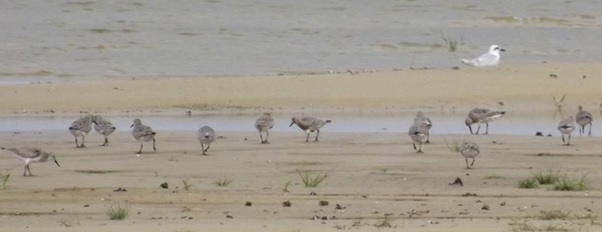
\includegraphics[width=0.75\linewidth]{imagens/cap07/Figura_7.7} 

}

\caption{Bando migratório neártico do maçarico-de-papo-vermelho (\emph{Calidris canutus}) na margem oeste da lagoa Mirim. Foto: Aurélea Mader}\label{fig:27}
\end{figure}



\textbf{Santa Catarina}

\textbf{53 - Municípios de Bocaina do Sul, Painel e Urupema}: esses municípios abrigam \href{https://youtu.be/-6shMIhlPN8}{importantes áreas de agregação de \emph{Amazona pretrei} no período não reprodutivo}, a partir do mês de maio, quando milhares de indivíduos se agregam em inúmeros sítios de pernoite (Schunck et al.~2011), a exemplo da localidade de Passo do Souza, que embora seja um imenso reflorestamento de \emph{Pinus} spp., em 2020 e 2021 foi local de pernoite de toda a população de \emph{A. pretrei}, com 22.332 papagaios (N. Prestes, com. pess. 2021).

\textbf{54 - Coxilha Rica e Estância do Meio}: principal área reprodutiva de \emph{Sporophila beltoni} em Santa Catarina. Destaca-se a área a oeste do rio Lava Tudo, na região da Coxilha Rica, com ocorrência de \emph{S. hypoxantha} e \emph{S. melanogaster}. A leste deste rio, a localidade de Estância do Meio contempla número muito significativo de territórios reprodutivos de \emph{S. beltoni} (M. Repenning \& C. Fontana, com. pess. 2021).

\textbf{55 - Ilhas marinhas costeiras da Deserta (Reserva Biológica Arvoredo), Moleques do Sul (Parque Estadual do Tabuleiro) e ilhas Itacolomis}: constituem áreas de pouso e reprodução de \emph{Sterna hirundinacea}, \emph{S. hirundo} e \emph{Thalasseus acuflavidus}, com avistamentos que chegam a centenas de indivíduos (Branco et al.~2004).

\textbf{56 - Foz do rio Tijucas}: área de alimentação de várias espécies migratórias. Área de agregação de grandes bandos de espécies migratórias, por exemplo, \emph{Plegadis chihi} (2.000 indivíduos), \emph{Charadrius semipalmatus} (200), \emph{Calidris fuscicollis} (200), \emph{Rynchops niger} (200), \emph{Calidris canutus} (112) e \emph{Thalasseus acuflavidus} (60). Também são observados grupos menores de \emph{Calidris pusilla}, \emph{C. alba}, \emph{Pluvialis squatarola}, \emph{Tringa melanoleuca} e \emph{T. flavipes} (F. Fisch \& A. Roos, com. pess. 2021; Ebird-Tijucas-Foz do rio Tijucas 2022).

\textbf{57 - Praias entre a foz do rio Urussanga e a foz do rio Araranguá}: trecho entre os municípios de Balneário Rincão (Figura \ref{fig:28}) e Araranguá. A importância dessa região litorânea para a avifauna migratória e limícola já é mencionada há pelo menos três décadas (Rosário-Bege \& Marterer 1991). Recentes estudos confirmam tal indicação (Branco et al.~2004, Romagna 2015, Gava-Just et al.~2018). Por exemplo, das 28 espécies listadas no ``Plano de Ação Nacional para Conservação das Aves Limícolas Migratórias'', 18 possuem ocorrência confirmada nas praias entre as fozes do rio Urussanga e Araranguá (Gava-Just et al.~2018, WikiAves 2021). A região serve como área de alimentação, descanso e abrigo para Scolopacidae e Sterninae, incluindo espécies ameaçadas de extinção como \emph{Calidris canutus} (bandos de até 160 indivíduos, em abril de 2014) e \emph{Sterna hirundinacea} (bandos de até 650 indivíduos, em julho de 2014). Destaque ainda para grandes concentrações de \emph{Calidris alba}, com contagem máxima de 2.500 indivíduos no outono de 2018. Outros migrantes neárticos, como \emph{Charadrius semipalmatus}, \emph{Calidris fuscicollis}, \emph{Tringa flavipes}, \emph{Sterna hirundo} e \emph{Pluvialis dominica} ocorrem em bandos de dezenas de indivíduos. Além dos migrantes neárticos, pequenos bandos de migrantes austrais como \emph{Charadrius falklandicus}, \emph{Charadrius modestus} e \emph{Larus atlanticus} ocorrem regularmente na região (J. Gava-Just, com. pess. 2021)\\

\begin{figure}[H]

{\centering 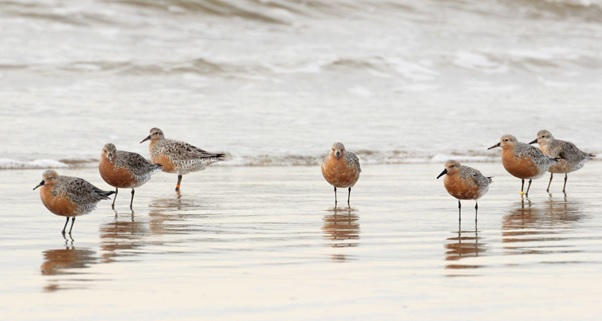
\includegraphics[width=0.75\linewidth]{imagens/cap07/Figura_7.8} 

}

\caption{Bando de maçarico-de-papo-vermelho (\emph{Calidris canutus}) no balneário Rincão. Foto: Rafael Romagna}\label{fig:28}
\end{figure}



\textbf{\emph{Zona pelágica}}

\textbf{58 - Ilhas oceânicas}: as ilhas oceânicas são, via de regra, áreas extremamente importantes para a avifauna marinha e migratória. Os arquipélagos de Fernando de Noronha (PE) e de Abrolhos (BA), o Atol das Rocas (RN) e as ilhas de Trindade e Martim Vaz (ES) são pontos críticos de pouso, descanso, alimentação e reprodução. \emph{Onychoprion fuscatus} nidifica em todas estas ilhas oceânicas (Figura \ref{fig:29}). O Arquipélago de Fernando de Noronha é, atualmente, o único local reprodutivo de \emph{Puffinus lherminieri} no Brasil. \emph{Pterodroma arminjoniana}, no Atlântico Sul, reproduz-se apenas em Trindade e Martim Vaz e o Atol das Rocas destaca-se por ser a área com a maior agregação de aves marinhas em nidificação no Brasil. Alguns migrantes também utilizam a área do Atol para repouso e alimentação: \emph{Pluvialis squatarola}, \emph{Charadrius semipalmatus}, \emph{Arenaria interpres}, \emph{Numenius hudsonicus} e \emph{Limnodromus griseus} (Sick 1997, Alves et al.~2004, Fonseca-Neto 2004, Bencke et al.~2006).

\begin{figure}[H]

{\centering 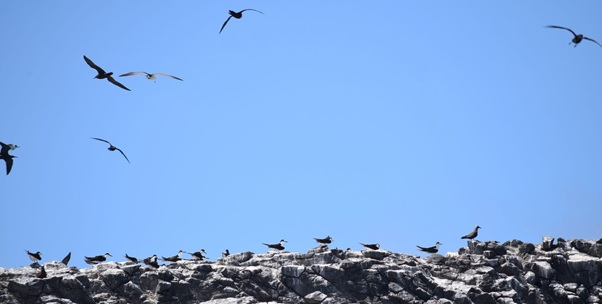
\includegraphics[width=0.75\linewidth]{imagens/cap07/Figura_7.9} 

}

\caption{Colônia de \emph{Onychoprion fuscatus}. Foto: Patrícia Serafini}\label{fig:29}
\end{figure}



\newpage

\hypertarget{uxe1reas-de-concentrauxe7uxe3o-de-aves-migratuxf3rias-mapa-final}{%
\section{Áreas de Concentração de Aves Migratórias: mapa final}\label{uxe1reas-de-concentrauxe7uxe3o-de-aves-migratuxf3rias-mapa-final}}

Considerando conjuntamente as áreas priorizadas com base na riqueza e sensibilidade de espécies migratórias (Zonation) e as áreas de agregação com expressivo número de indivíduos (revisão bibliográfica e consulta a especialistas), o mapa final de Áreas de Concentração de Aves Migratórias resultou na seleção de 2.149 células, totalizando 737.000 km² ou, aproximadamente, 8\% da superfície do Brasil (Figura \ref{fig:30}).

\begin{figure}[H]

{\centering 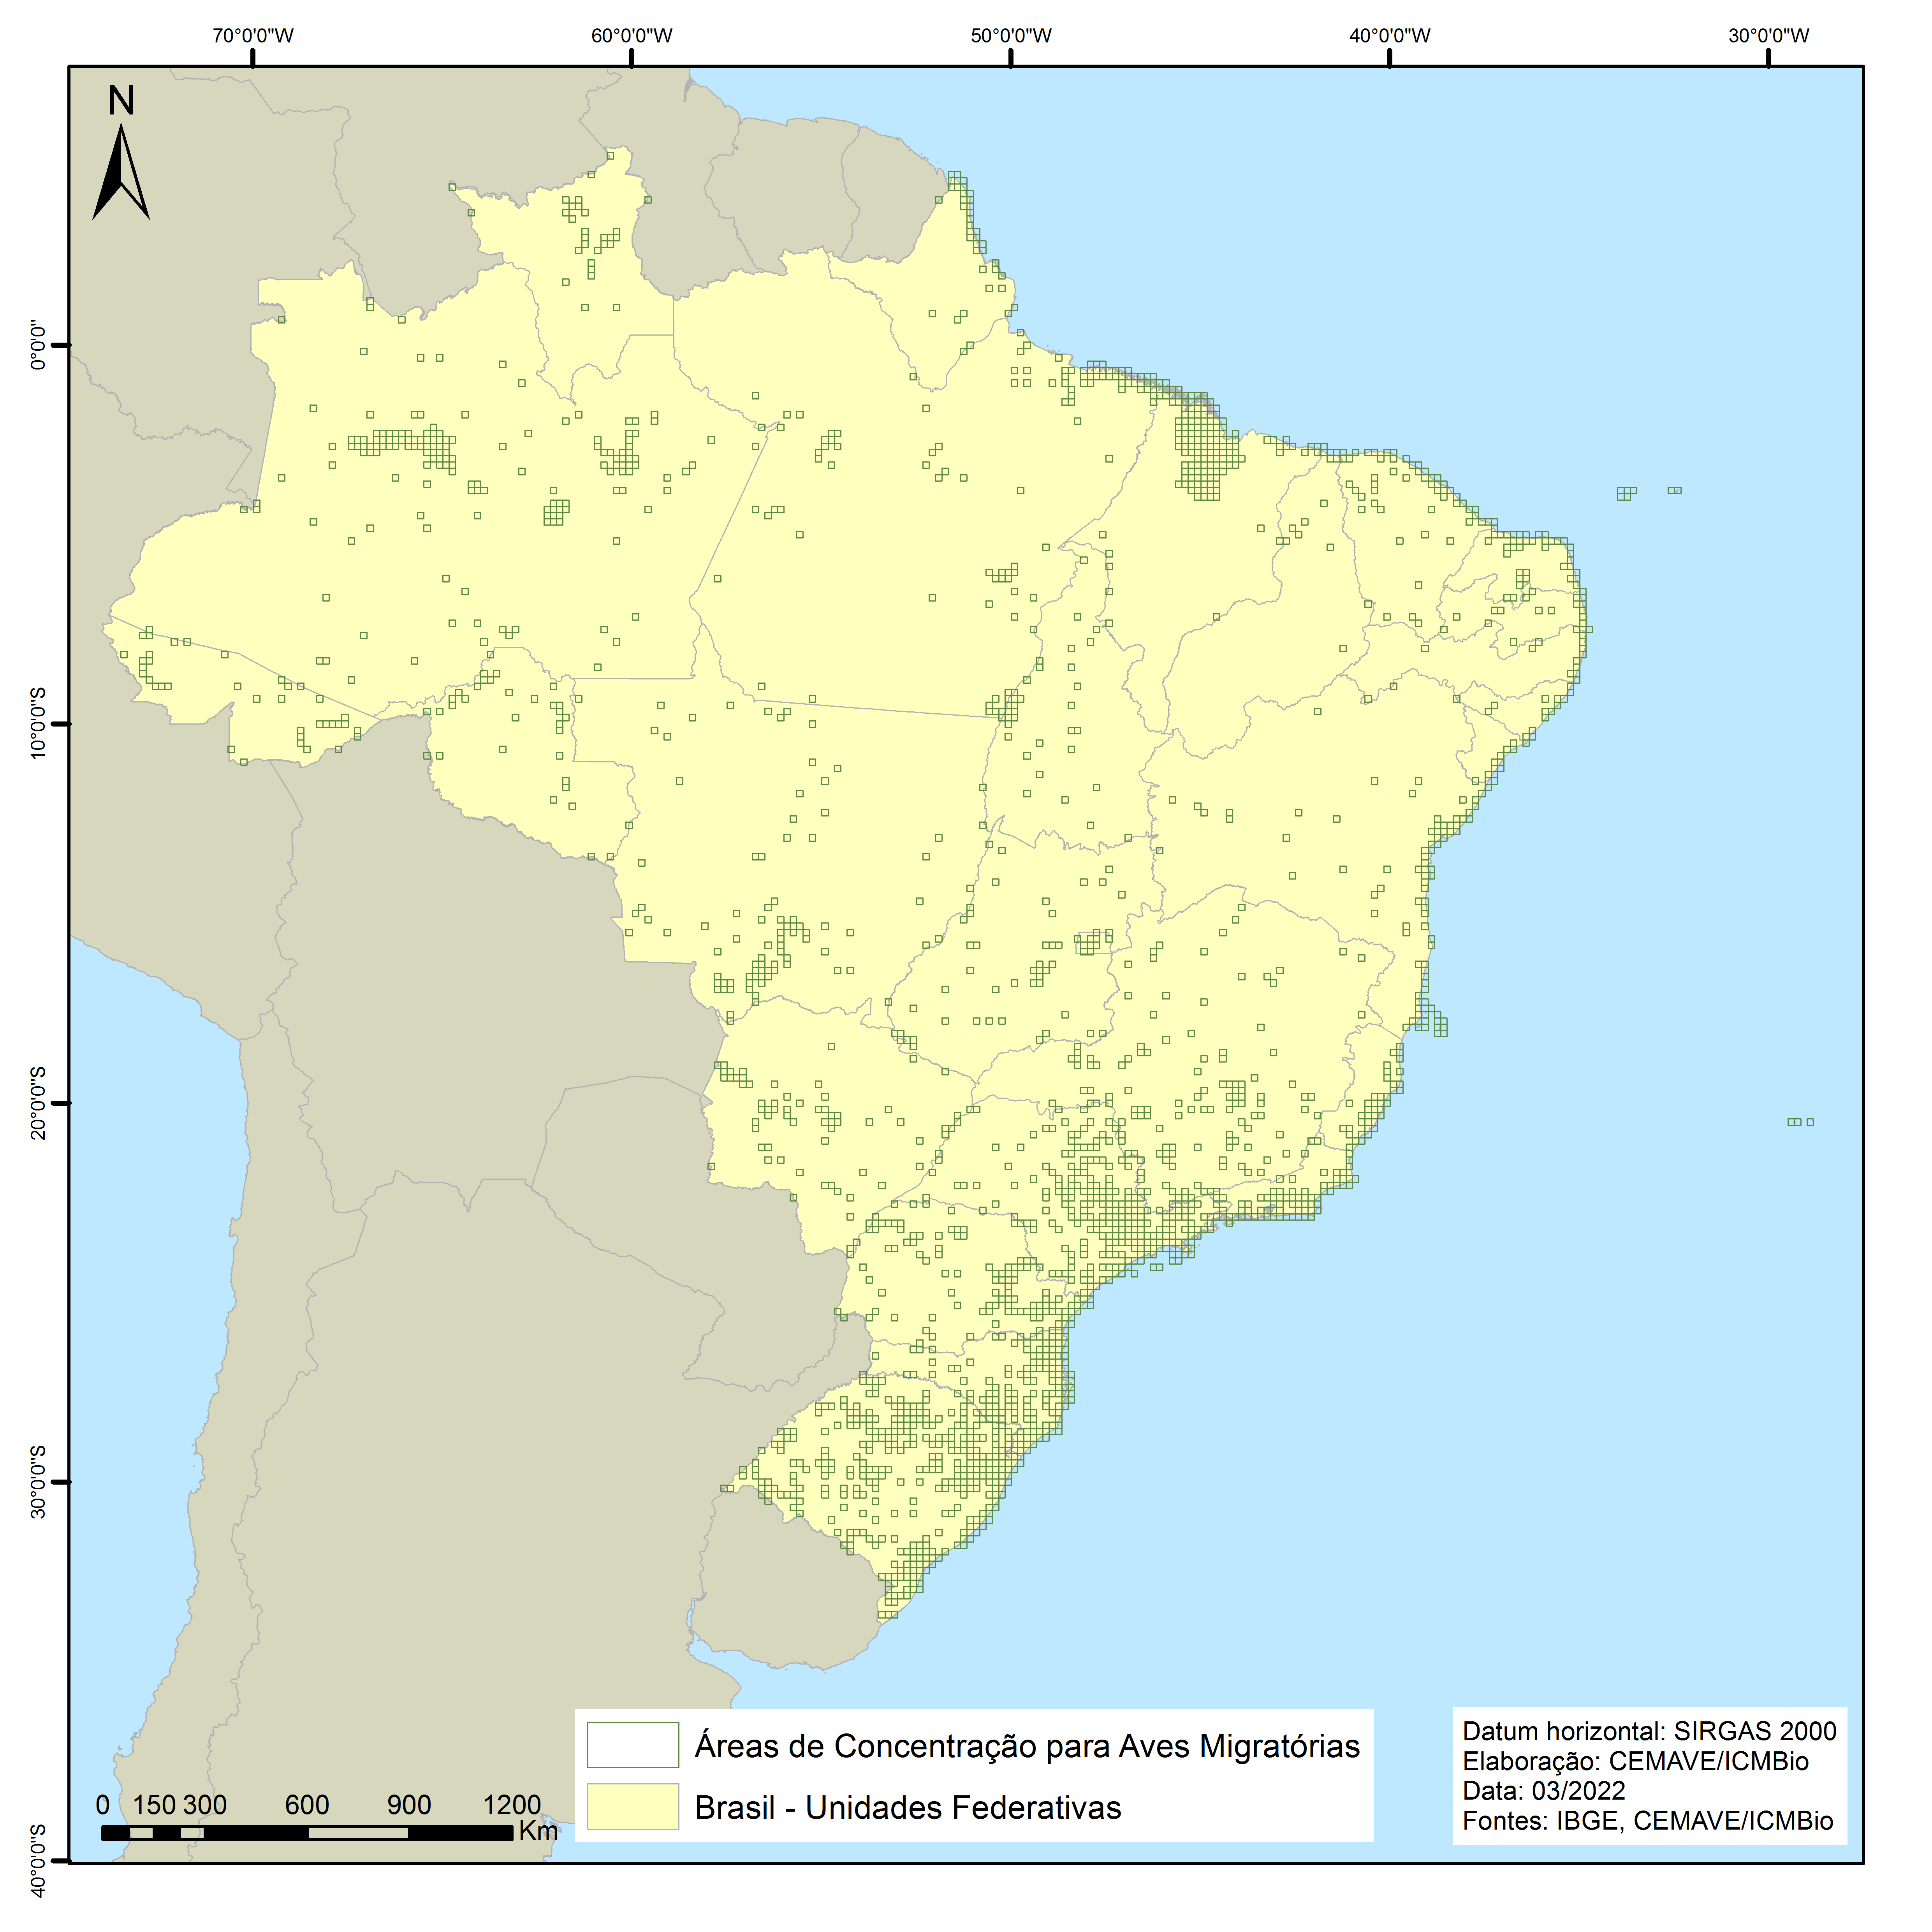
\includegraphics[width=0.75\linewidth]{imagens/cap07/Figura_7.10} 

}

\caption{Áreas de Concentração de Aves Migratórias no Brasil.}\label{fig:30}
\end{figure}

As Áreas de Concentração de Aves Migratórias estão disponíveis para \emph{download} em \href{https://www.icmbio.gov.br/cemave/destaques-e-noticias/240-cemave-publica-relatorio-sobre-rotas-de-aves-migratorias.html}{arquivos no formato *.shp}. Este relatório também pode ser encontrado no \href{https://www.gov.br/icmbio/pt-br}{Portal do ICMBio} na \emph{internet} e no \href{https://cemave-sede.github.io/painel-aves-migratorias/\#vis\%C3\%A3o-geral}{painel \emph{on-line}} criado especificamente para o compartilhamento de seu conteúdo. Mapas com maior detalhamento ilustrando as áreas selecionadas em cada estado por região e também as ilhas oceânicas são apresentados abaixo (Figuras \ref{fig:31} a \ref{fig:45}).

Cabe ressaltar que o planejamento sistemático para conservação por meio da priorização de áreas ocupadas por espécies sensíveis a determinado tipo de empreendimento não gera um produto definitivo. Além das óbvias evoluções metodológicas e tecnológicas que nos permitem refinar os produtos, é importante esclarecer que, no caso específico deste relatório, o conhecimento a respeito das migrações de aves ainda é limitado no Brasil. A dinâmica das migrações ajusta-se continuamente a inúmeras variáveis e em diferentes escalas, em decorrência de alterações em pequenos sítios na rota migratória, passando por flutuações populacionais resultantes de impactos em nível regional ou mesmo por alterações em resposta a mudanças climáticas globais.

Sendo assim, a priorização precisa ser constantemente revisada para que novos cenários sejam considerados e para que o planejamento esteja condizente com a realidade do momento. O aporte de críticas ao processo de análise e aos métodos aqui utilizados, bem como o compartilhamento de novas informações para alimentar esse modelo, são muito bem-vindos. Sabemos que este documento é resultado do empenho de muitas pessoas, mesmo que indiretamente, e esperamos que a colaboração entre aqueles que detêm conhecimento sobre nossa biodiversidade e as instituições que trabalham por sua conservação seja cada vez maior, a fim de que possamos gerar produtos cada vez melhores.

A seguir são apresentadas em detalhe as Áreas de Concentração de Aves Migratórias por unidade federativa.

\begin{figure}[H]

{\centering 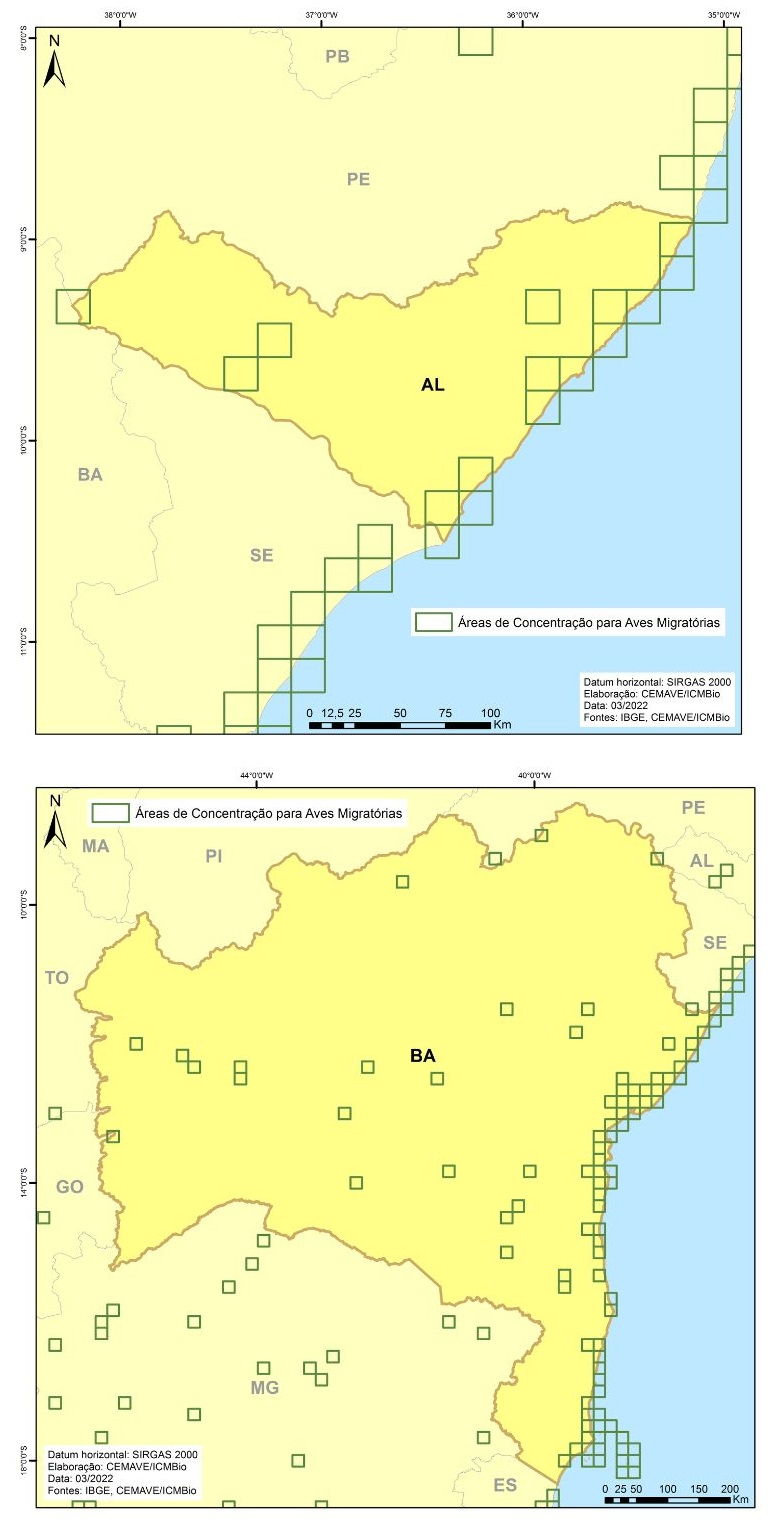
\includegraphics[width=0.7\linewidth]{imagens/cap07/Fig_11_AL_BA} 

}

\caption{Áreas de Concentração de Aves Migratórias nos estados de Alagoas (acima) e Bahia (abaixo).}\label{fig:31}
\end{figure}

\begin{figure}[H]

{\centering 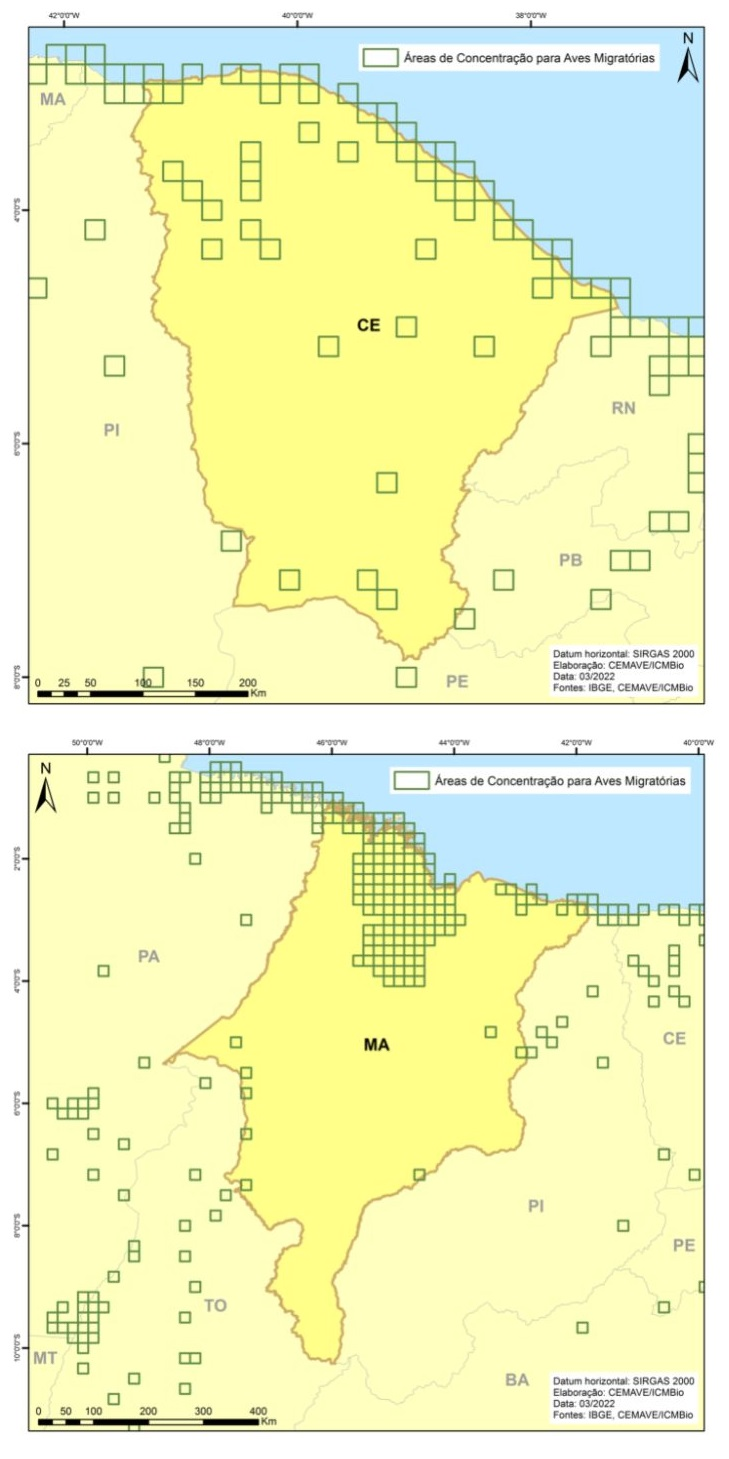
\includegraphics[width=0.7\linewidth]{imagens/cap07/Fig_12_CE_MA} 

}

\caption{Áreas de Concentração de Aves Migratórias nos estados do Ceará (acima) e Maranhão (abaixo).}\label{fig:32}
\end{figure}

\begin{figure}[H]

{\centering 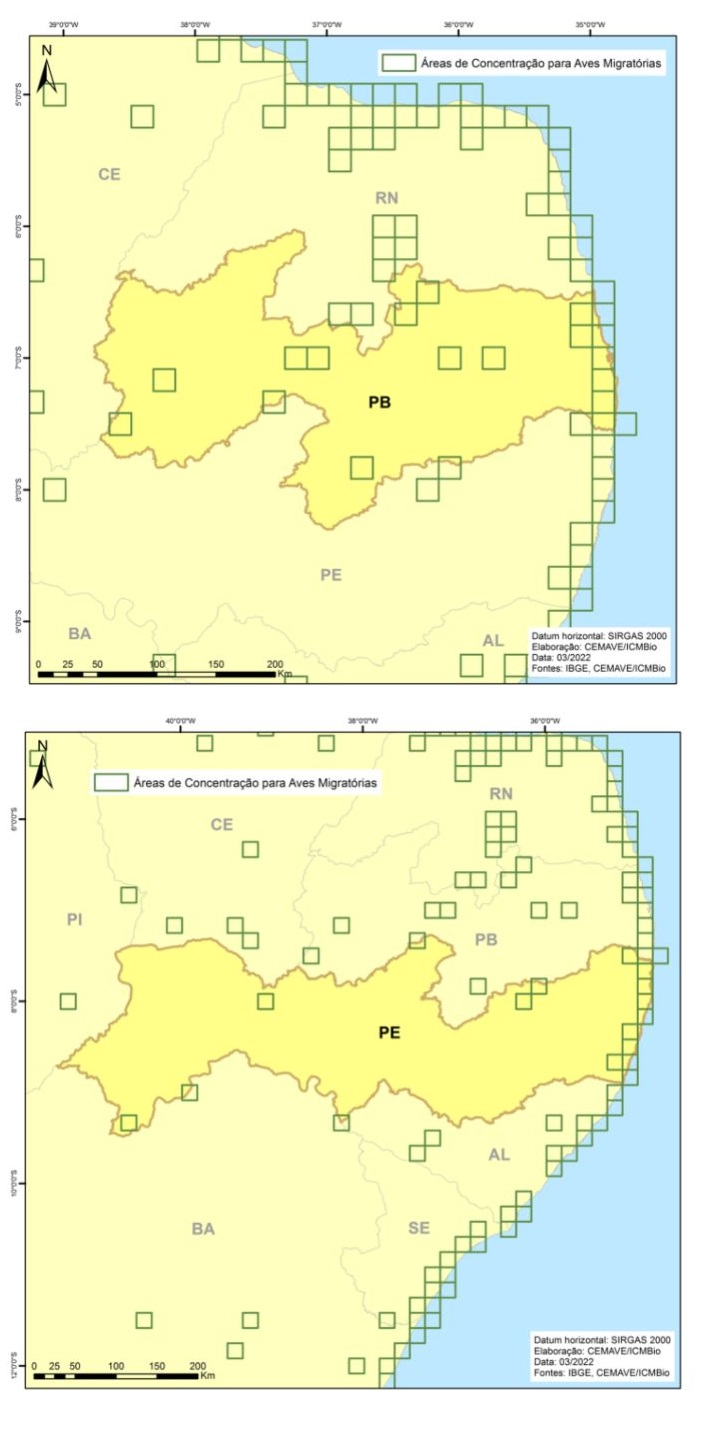
\includegraphics[width=0.7\linewidth]{imagens/cap07/Fig_13_PB_PE} 

}

\caption{Áreas de Concentração de Aves Migratórias nos estados da Paraíba (acima) e Pernambuco (abaixo).}\label{fig:33}
\end{figure}

\begin{figure}[H]

{\centering 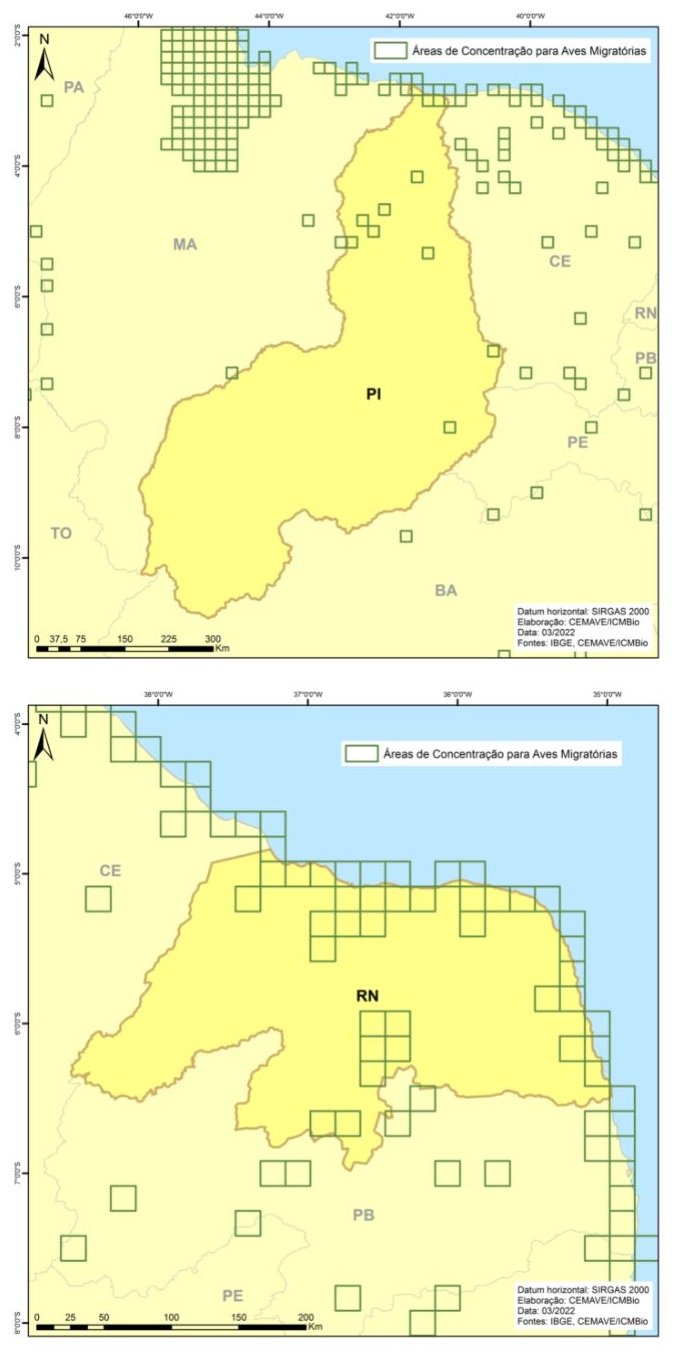
\includegraphics[width=0.7\linewidth]{imagens/cap07/Fig_14_PI_RN} 

}

\caption{Áreas de Concentração de Aves Migratórias nos estados do Piauí (acima) e Rio Grande do Norte (abaixo).}\label{fig:34}
\end{figure}

\begin{figure}[H]

{\centering 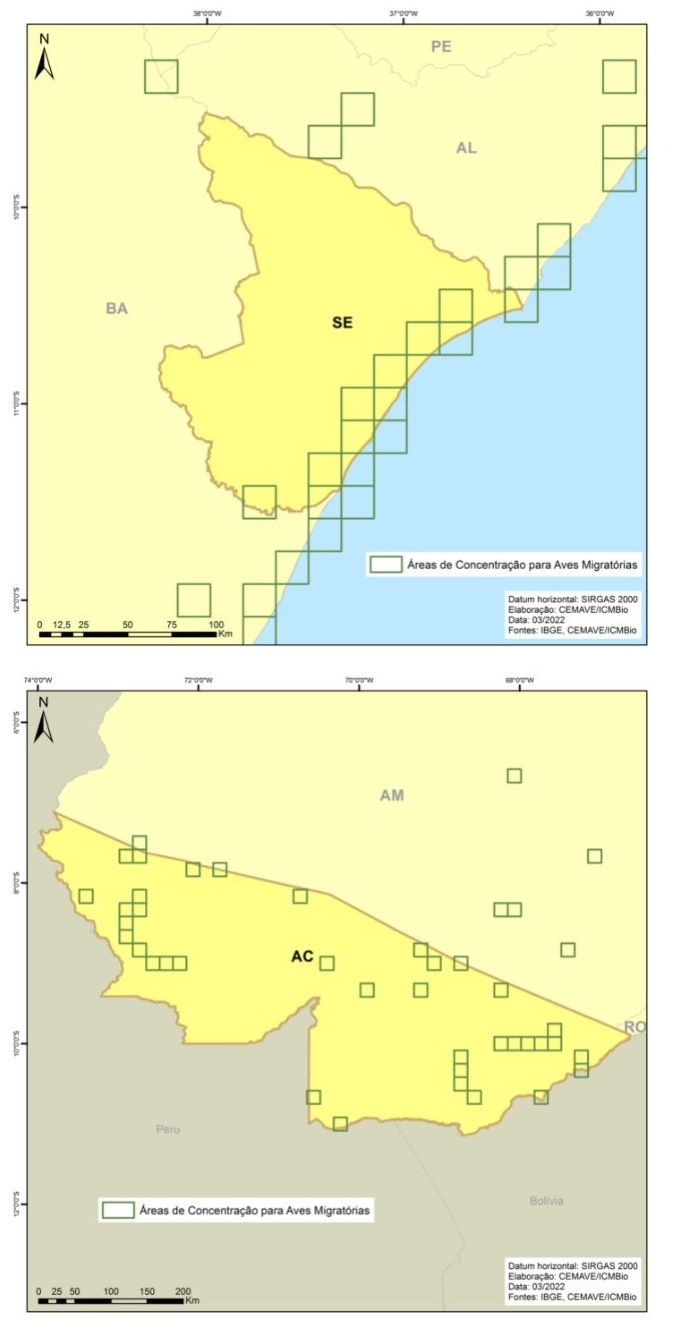
\includegraphics[width=0.7\linewidth]{imagens/cap07/Fig_15_SE_AC} 

}

\caption{Áreas de Concentração de Aves Migratórias nos estados de Sergipe (acima) e Acre (abaixo).}\label{fig:35}
\end{figure}

\begin{figure}[H]

{\centering 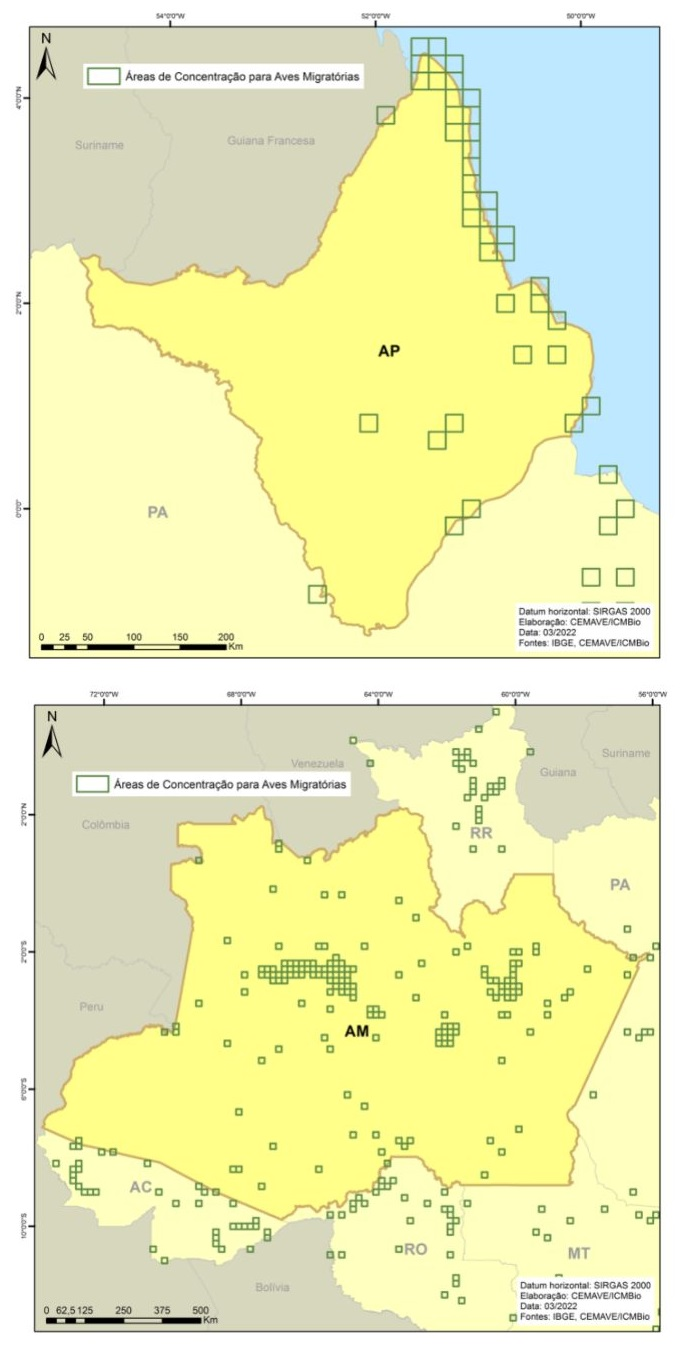
\includegraphics[width=0.7\linewidth]{imagens/cap07/Fig_16_AP_AM} 

}

\caption{Áreas de Concentração de Aves Migratórias nos estados do Amapá (acima) e Amazonas (abaixo).}\label{fig:36}
\end{figure}

\begin{figure}[H]

{\centering 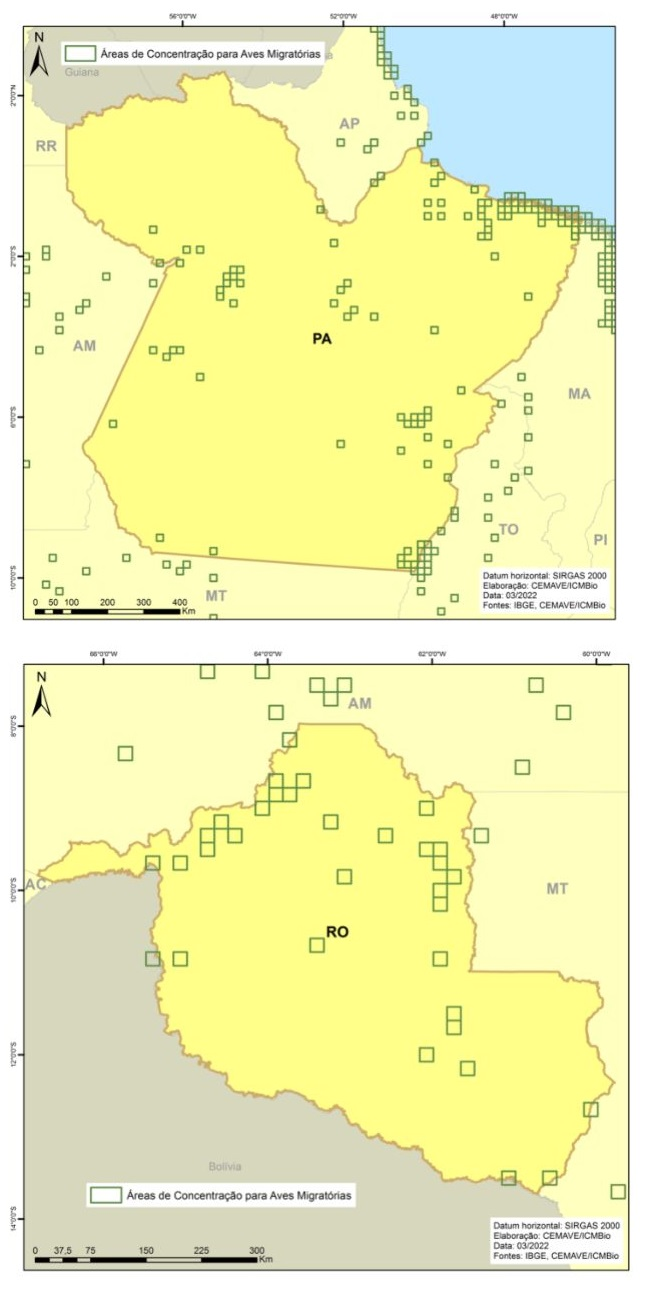
\includegraphics[width=0.7\linewidth]{imagens/cap07/Fig_17_PA_RO} 

}

\caption{Áreas de Concentração de Aves Migratórias nos estados do Pará (acima) e Rondônia (abaixo).}\label{fig:37}
\end{figure}

\begin{figure}[H]

{\centering 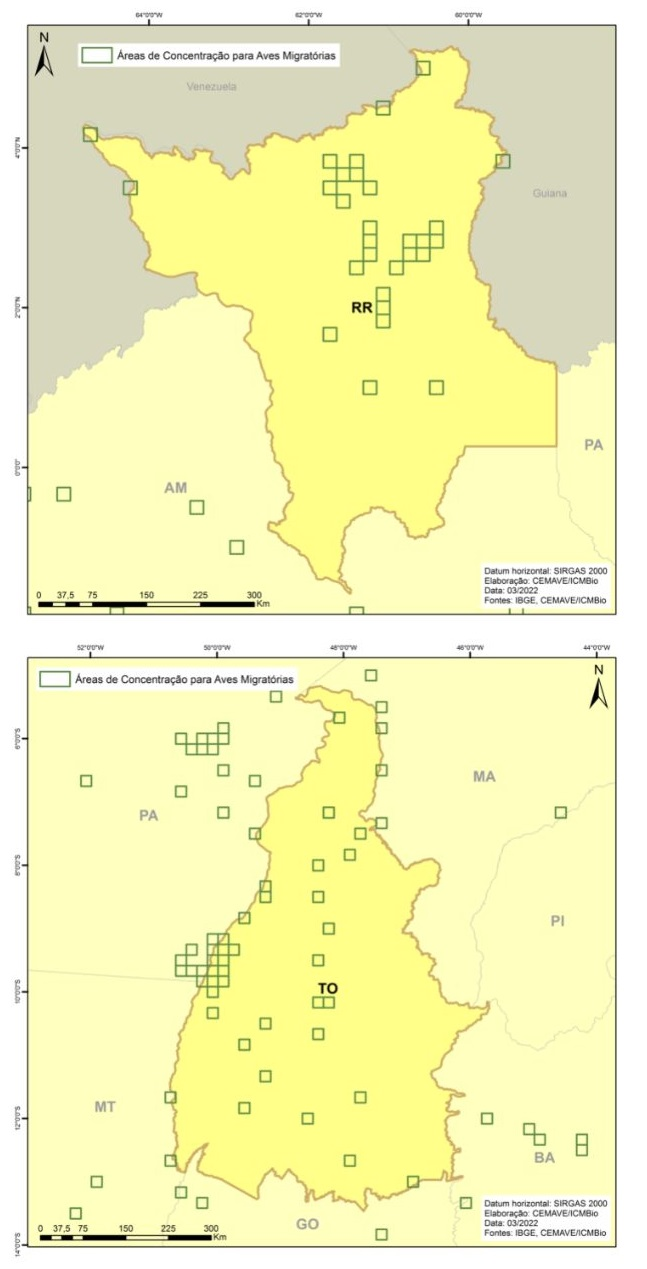
\includegraphics[width=0.7\linewidth]{imagens/cap07/Fig_18_RR_TO} 

}

\caption{Áreas de Concentração de Aves Migratórias nos estados de Roraima (acima) e Tocantins (abaixo).}\label{fig:38}
\end{figure}

\begin{figure}[H]

{\centering 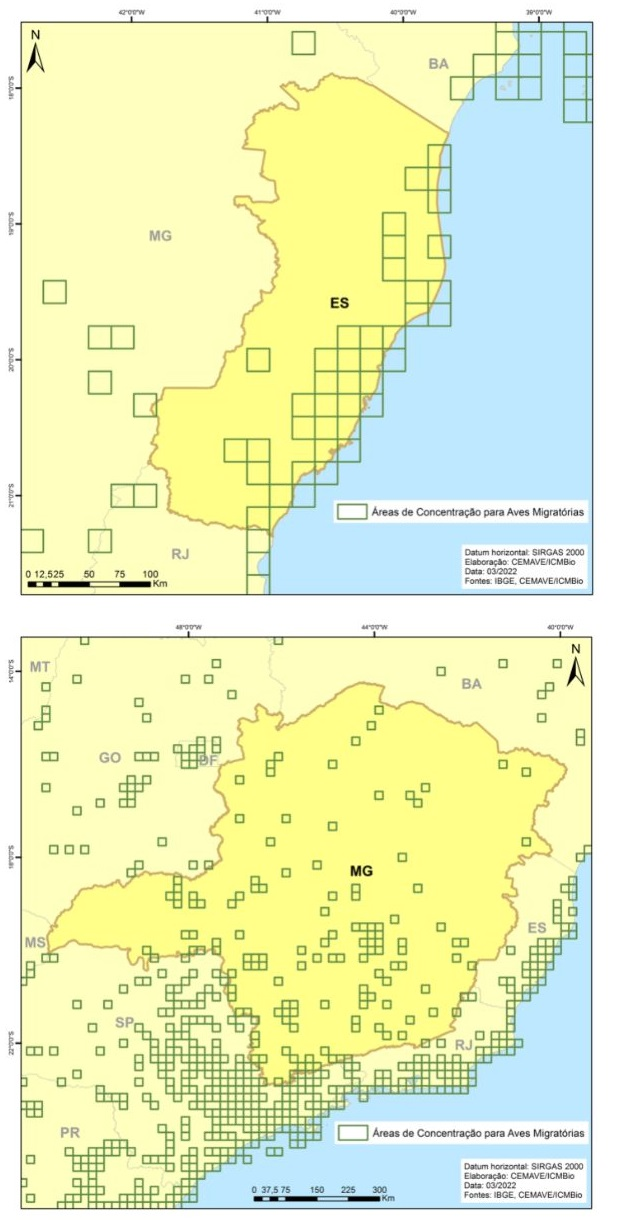
\includegraphics[width=0.7\linewidth]{imagens/cap07/Fig_19_ES_MG} 

}

\caption{Áreas de Concentração de Aves Migratórias nos estados do Espírito Santo (acima) e Minas Gerais (abaixo).}\label{fig:39}
\end{figure}

\begin{figure}[H]

{\centering 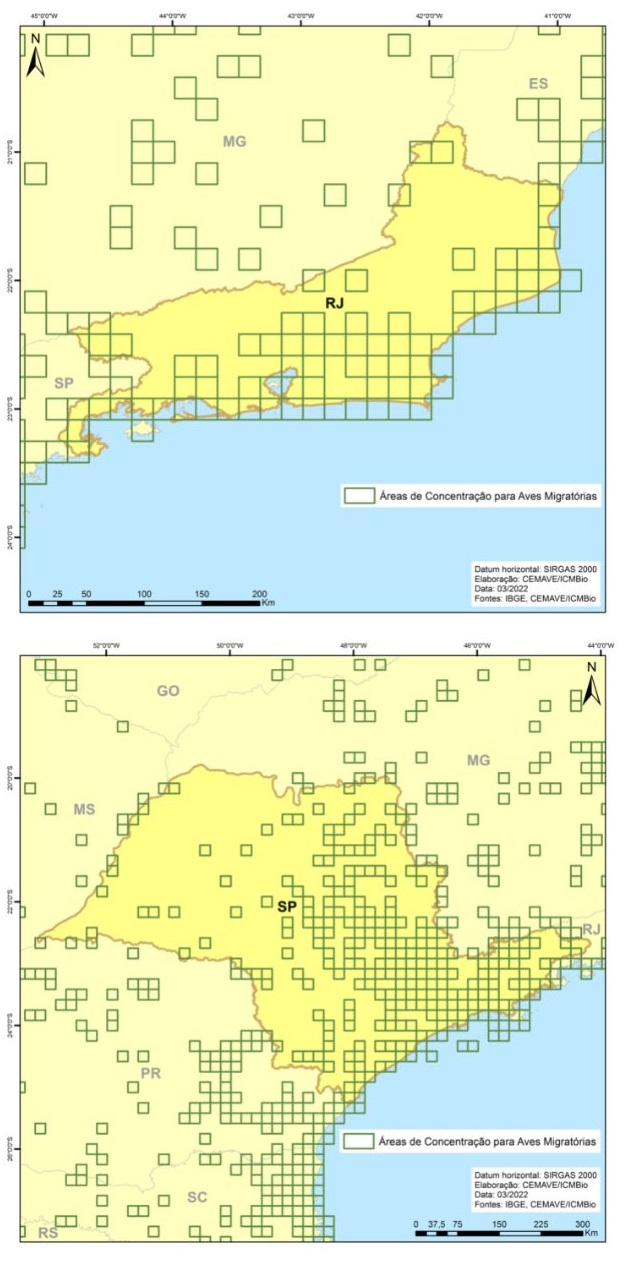
\includegraphics[width=0.7\linewidth]{imagens/cap07/Fig_20_RJ_SP} 

}

\caption{Áreas de Concentração de Aves Migratórias nos estados do Rio de Janeiro (acima) e São Paulo (abaixo).}\label{fig:40}
\end{figure}

\begin{figure}[H]

{\centering 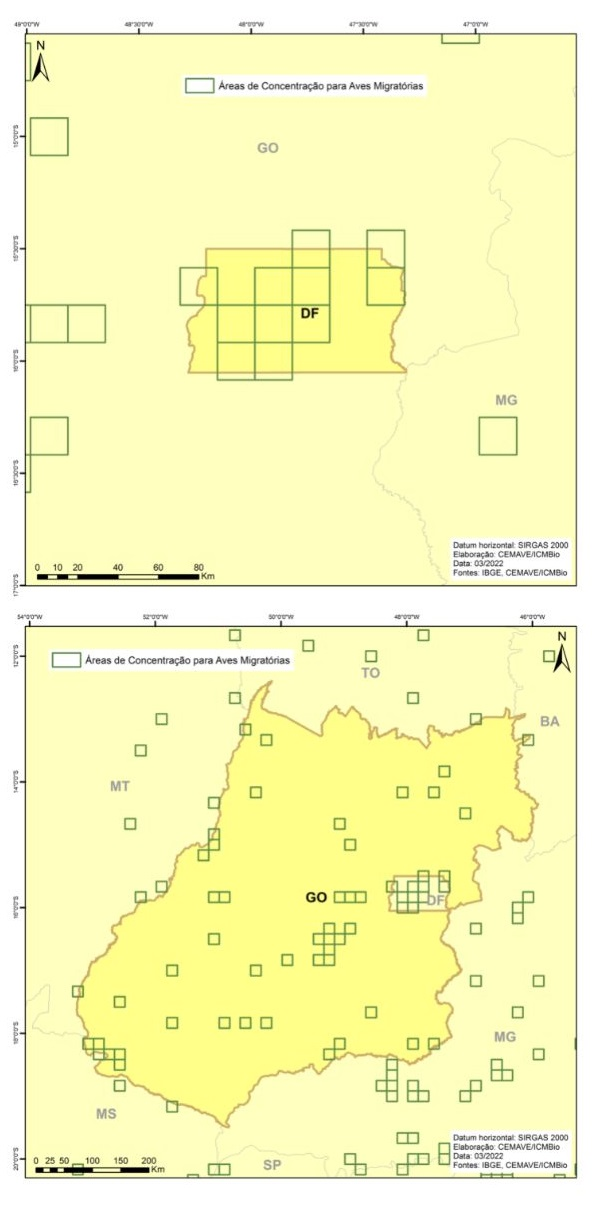
\includegraphics[width=0.7\linewidth]{imagens/cap07/Fig_21_DF_GO} 

}

\caption{Áreas de Concentração de Aves Migratórias no Distrito Federal (acima) e no estado de Goiás (abaixo).}\label{fig:41}
\end{figure}

\begin{figure}[H]

{\centering 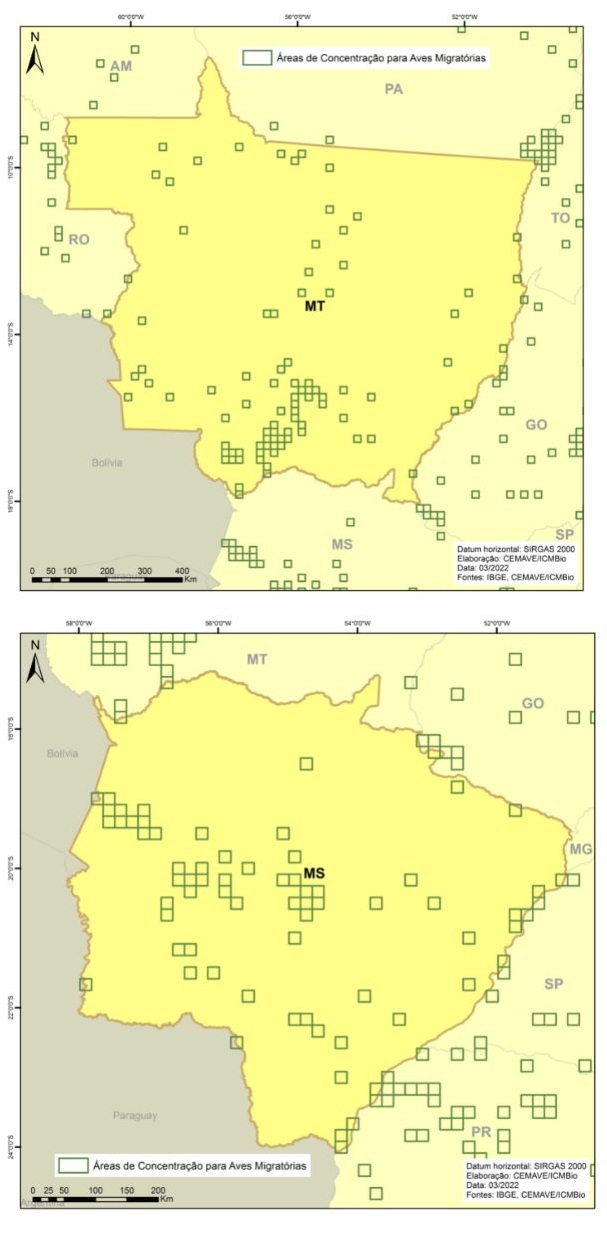
\includegraphics[width=0.7\linewidth]{imagens/cap07/Fig_22_MT_MS} 

}

\caption{Áreas de Concentração de Aves Migratórias nos estados de Mato Grosso (acima) e Mato Grosso do Sul (abaixo).}\label{fig:42}
\end{figure}

\begin{figure}[H]

{\centering 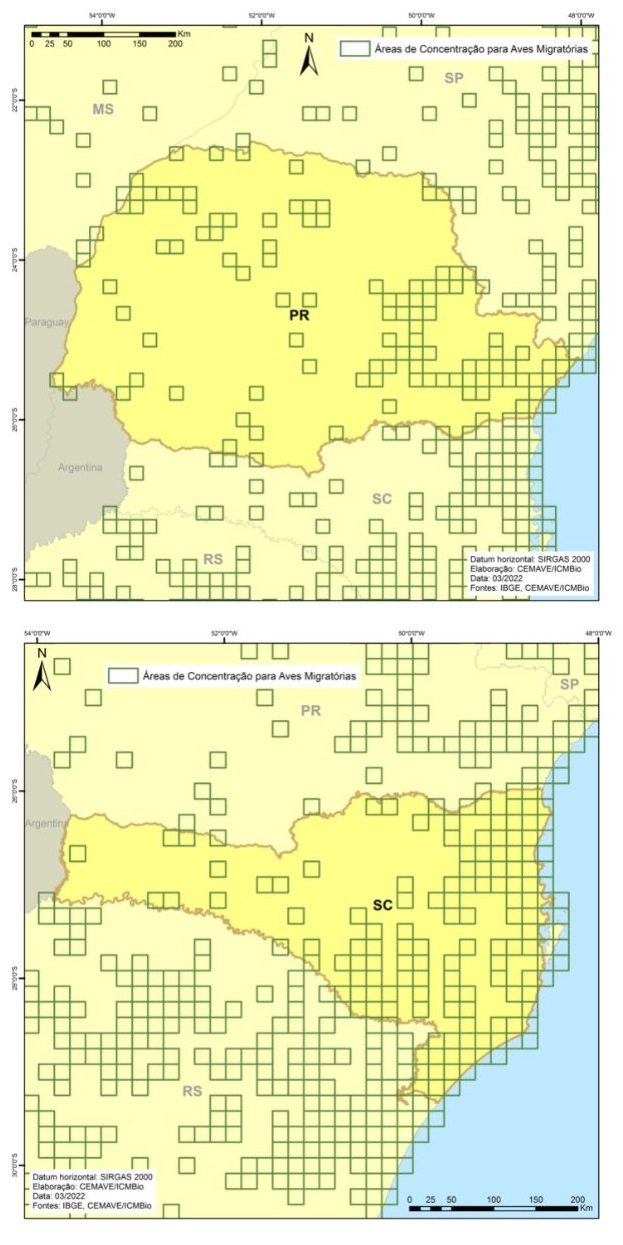
\includegraphics[width=0.7\linewidth]{imagens/cap07/Fig_23_PR_SC} 

}

\caption{Áreas de Concentração de Aves Migratórias nos estados do Paraná (acima) e Santa Catarina (abaixo).}\label{fig:43}
\end{figure}

\begin{figure}[H]

{\centering 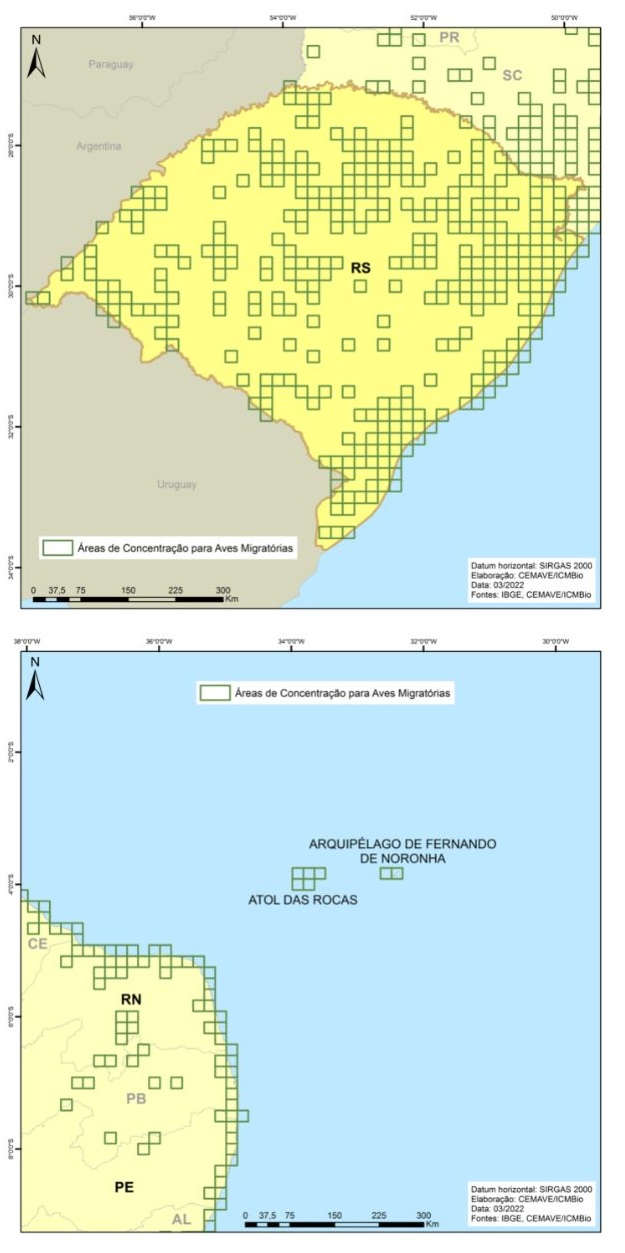
\includegraphics[width=0.7\linewidth]{imagens/cap07/Fig_24_RS_FN} 

}

\caption{Áreas de Concentração de Aves Migratórias no estado do Rio Grande do Sul (acima), no arquipélago de Fernando de Noronha e no atol das Rocas (abaixo).}\label{fig:44}
\end{figure}

\begin{figure}[H]

{\centering 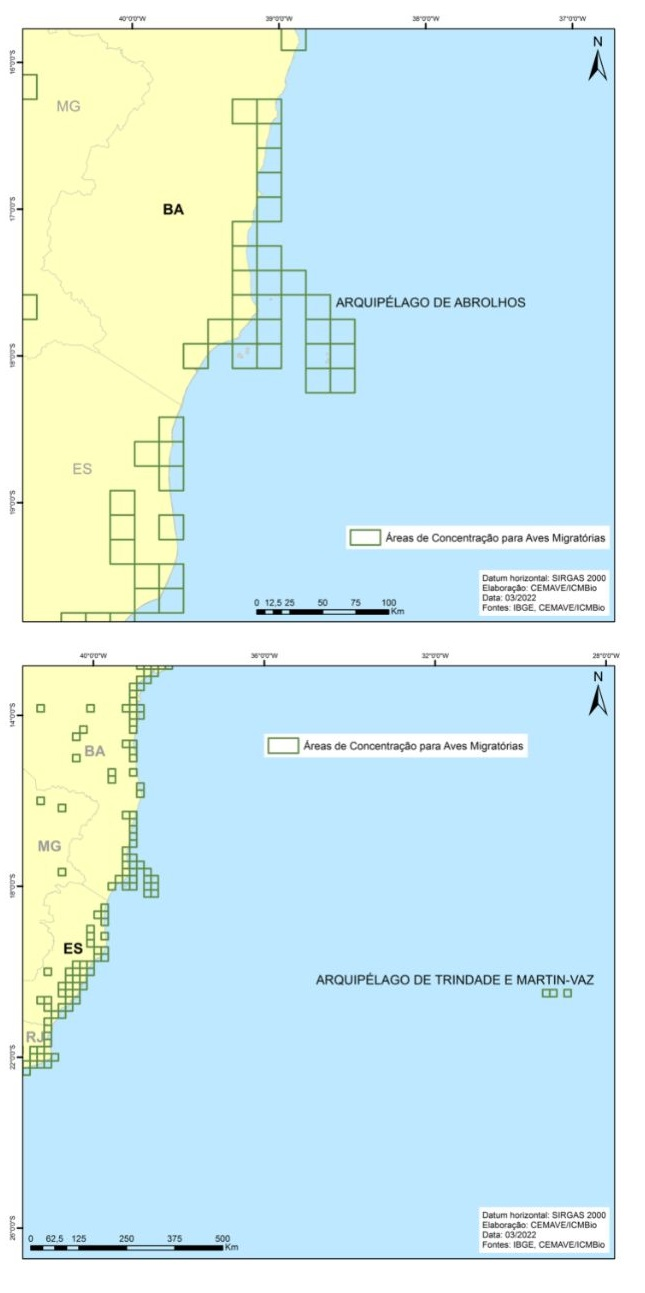
\includegraphics[width=0.7\linewidth]{imagens/cap07/Fig_25_AB_MV} 

}

\caption{Áreas de Concentração de Aves Migratórias nos arquipélagos de Abrolhos (acima) e Trindade e Martim-Vaz (abaixo).}\label{fig:45}
\end{figure}

\begin{blackbox}

\begin{center}
\textbf{AEROGERADORES: UMA BREVE ANÁLISE SOBRE O POTENCIAL ``EFEITO DE BARREIRA'' À FAUNA VOADORA}

\end{center}

A geração de energia a partir dos ventos é ambientalmente interessante e parece ser uma tendência a ser seguida. Contudo, alguns efeitos negativos podem surgir e cabe aos técnicos e gestores a análise e proposição de medidas que agreguem ainda mais sustentabilidade a esta atividade.

O capítulo 4 deste relatório traz os principais impactos, diretos e indiretos, relativos à instalação e operação de parques eólicos. Mesmo considerando as boas práticas na construção e gestão desses empreendimentos, que visam mitigar esses efeitos negativos, busca-se aqui ampliar a ótica de análise de um dos impactos diretos então citados: o efeito de barreira. Trata-se de uma breve análise relacionada à distribuição espacial das estruturas das torres eólicas e a área acumulada de varredura das suas pás e seu efeito de potencial obstáculo à fauna voadora.

Informações obtidas no \href{https://sigel.aneel.gov.br/Down}{sítio eletrônico da ANEEL} revelam a existência de 18.129 aerogeradores instalados na área continental do Brasil (\emph{download} do \emph{shapefile} ``Aerogeradores'' em 26 janeiro de 2022). Esses aerogeradores estão localizados em 13 estados brasileiros em quantidades muito variadas (Tabela \ref{tab:tab06}), mas com sua distribuição espacial bastante concentrada em algumas áreas (Figura \ref{fig:61a}, sendo a Bahia e o Rio Grande no Norte os estados com o maior número.

\end{blackbox}

\begin{figure}[H]

{\centering 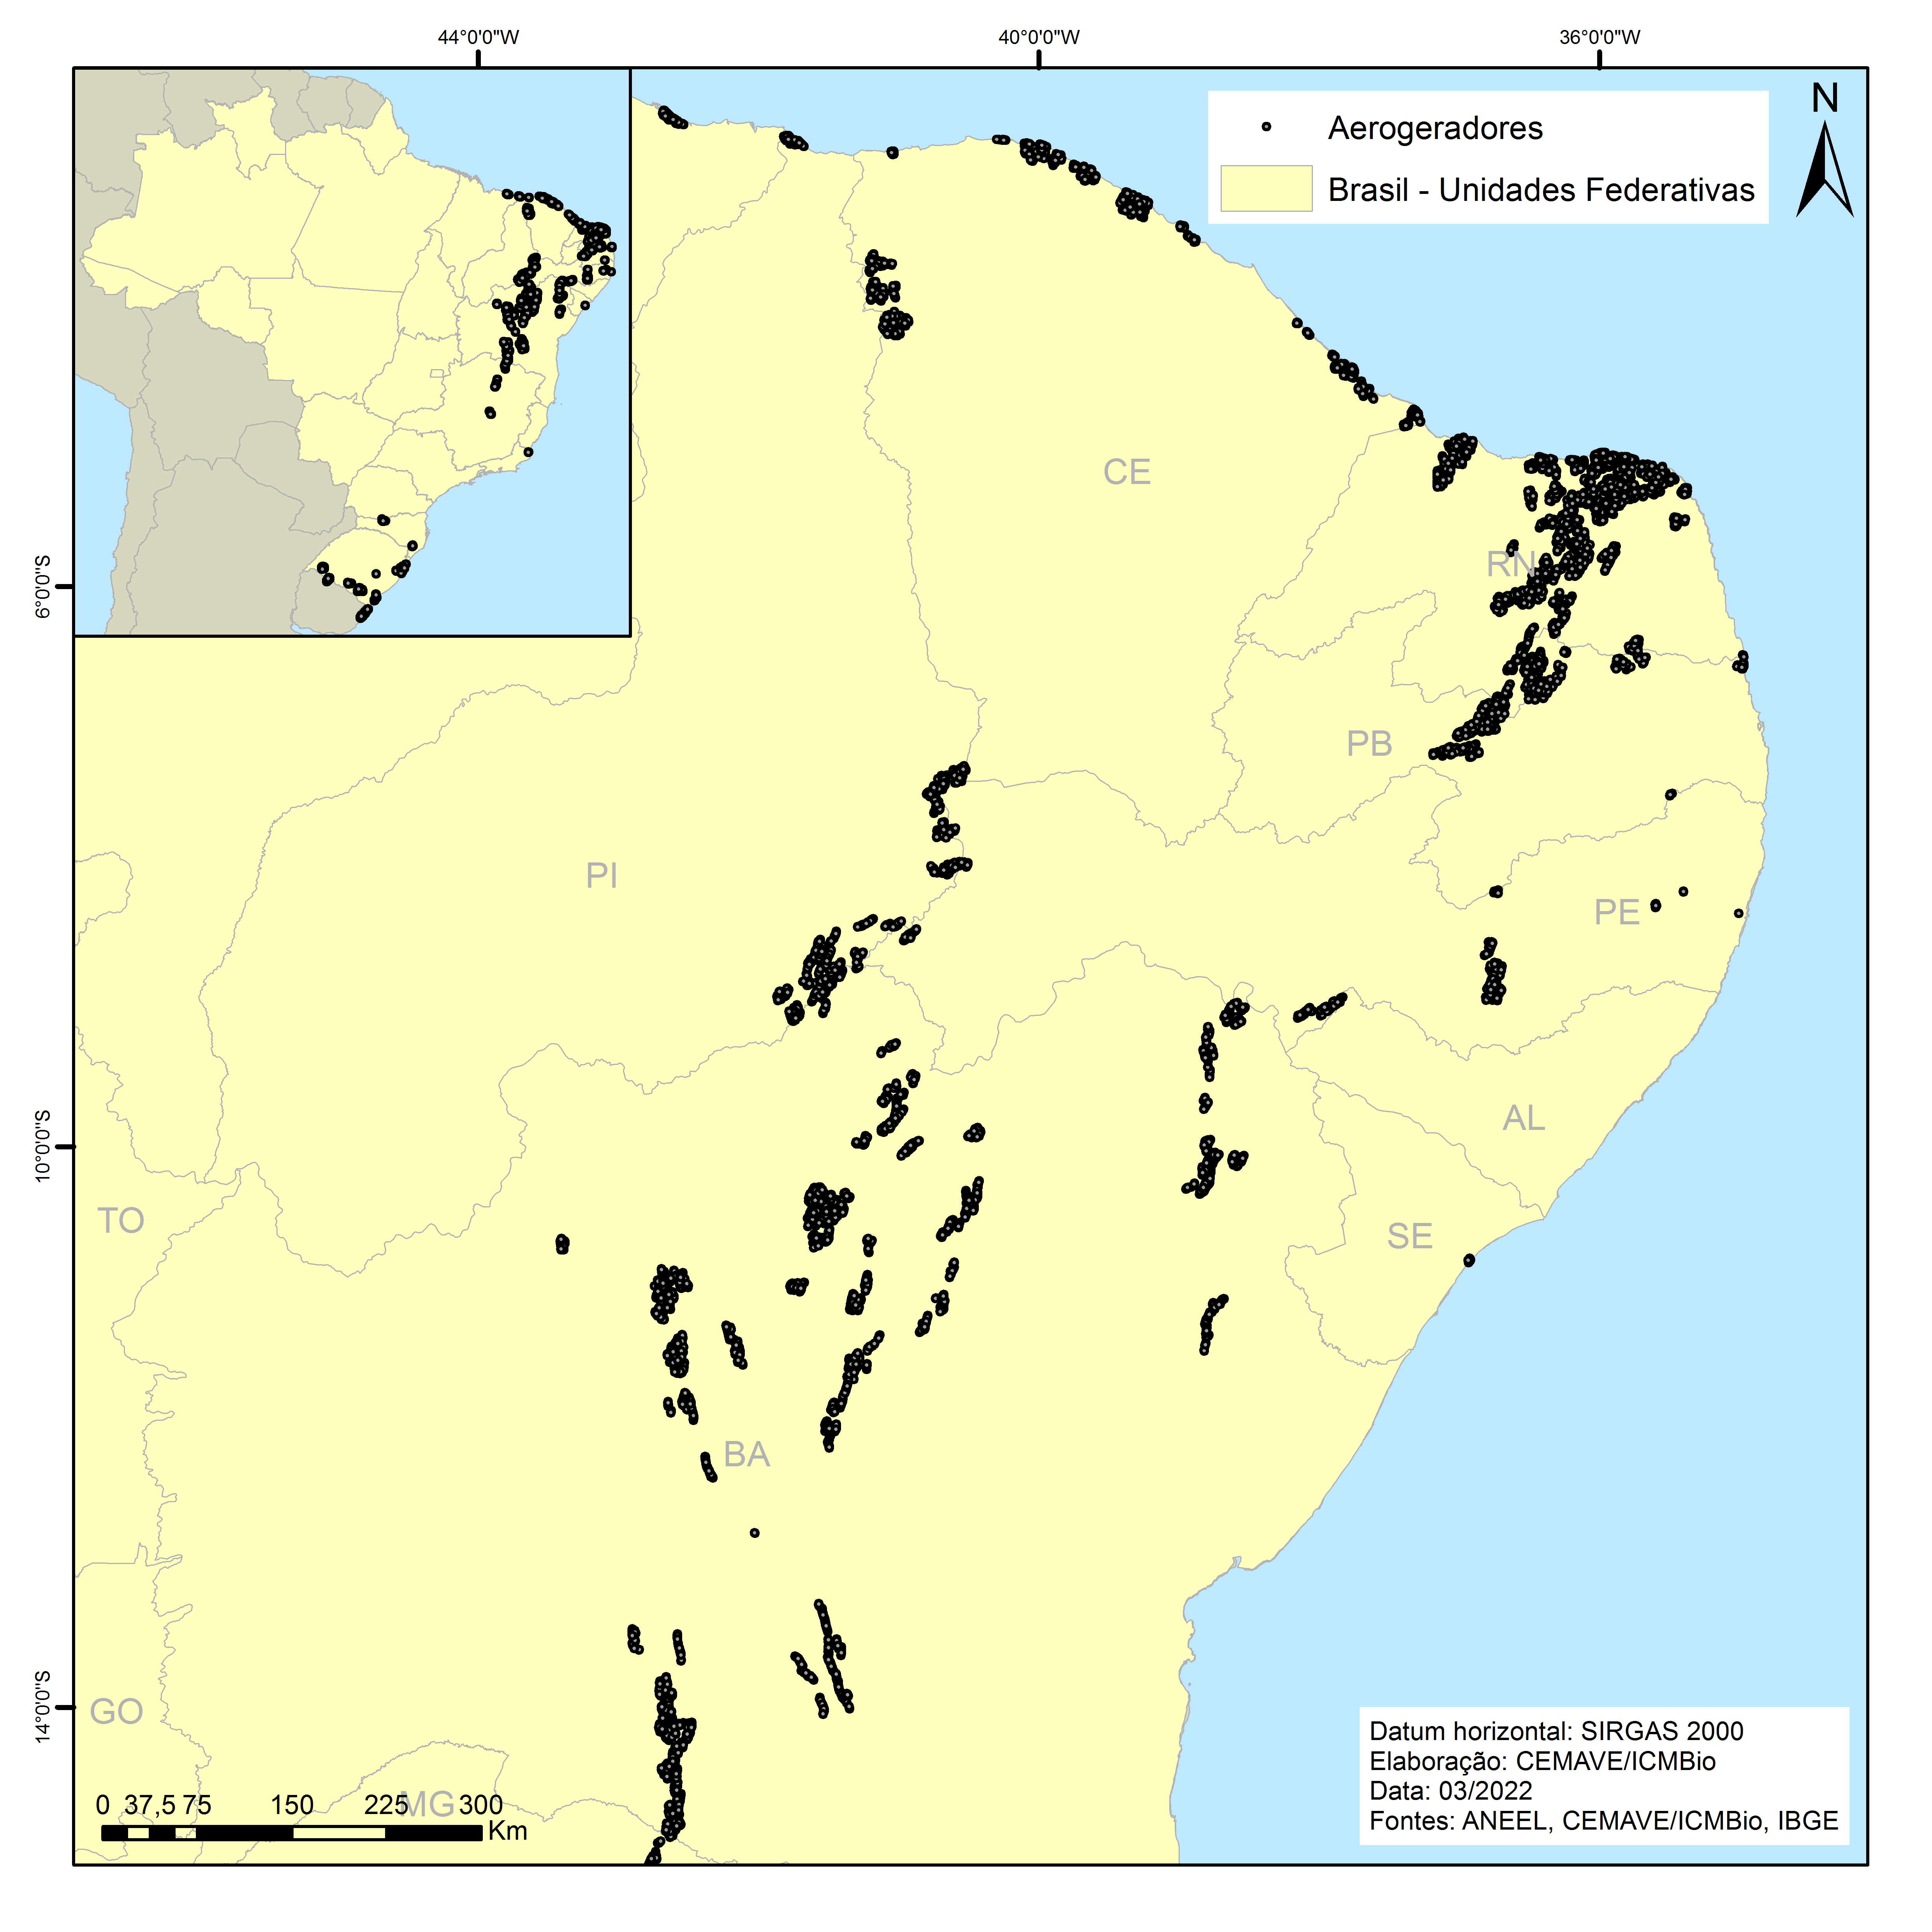
\includegraphics[width=0.75\linewidth]{imagens/cap07/Figura_7.41} 

}

\caption{. Distribuição dos aerogeradores nos estados da Bahia, Ceará, Maranhão, Paraíba, Pernambuco, Piauí, Rio Grande do Norte e Sergipe.}\label{fig:61a}
\end{figure}

\begin{blackbox}
A grande concentração de aerogeradores em determinados locais pode representar obstáculos para animais que voam nas faixas de altura dos seus rotores. Isto aconteceria devido à disposição espacial das grandes estruturas construídas em linhas, frequentemente paralelas, que muitas vezes se distribuem numa sequência (Figura \ref{fig:61b}), além, principalmente, do tamanho de suas pás, que podem ultrapassar os 150 metros de diâmetro de rotor.

Assim, a área de varredura das pás em movimento é um fator determinante na constituição de impactos à fauna voadora, como o efeito de barreira, pois se projeta verticalmente na faixa de voo como um grande obstáculo, que pode causar injúria ou mortalidade por colisão, sendo potencializado nos locais com maior adensamento de aerogeradores. O efeito cumulativo e sinérgico de empreendimentos próximos também merece atenção no planejamento regional (SNH 2012).

\end{blackbox}

\begin{figure}[H]

{\centering 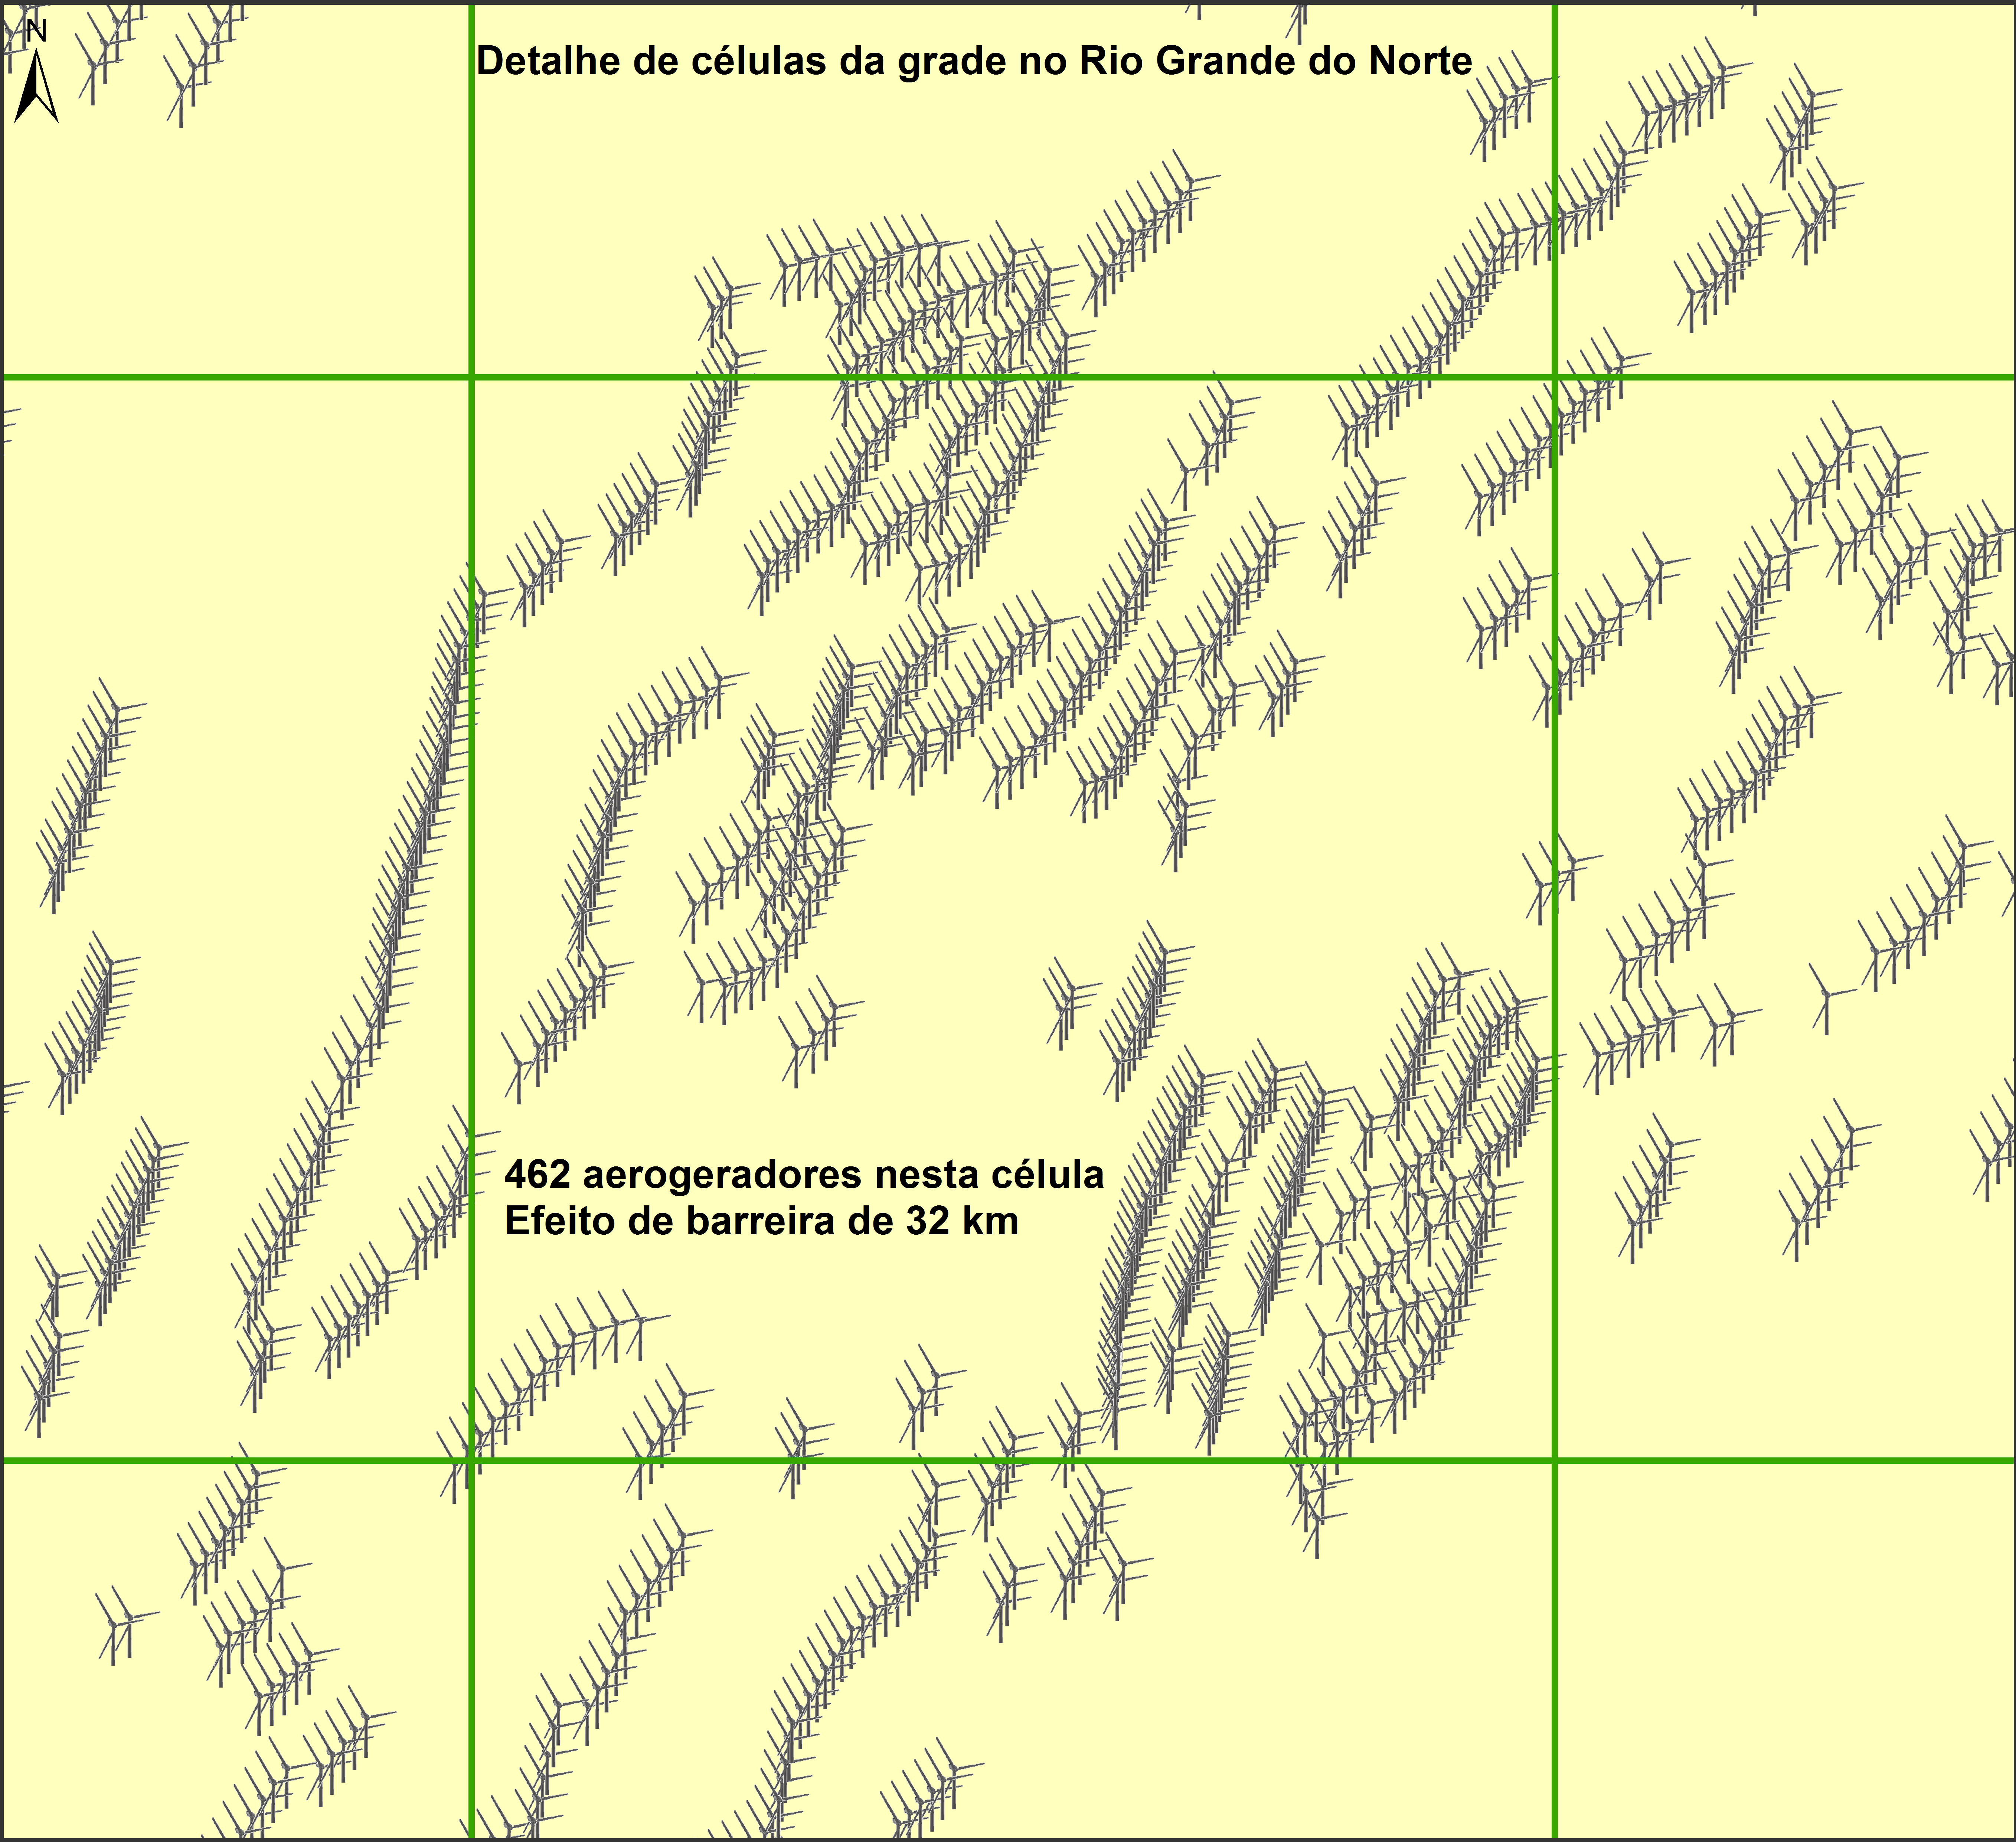
\includegraphics[width=0.75\linewidth]{imagens/cap07/Figura_7.42} 

}

\caption{Representação em detalhe da distribuição espacial de aerogeradores em uma célula da grade de análise no Rio Grande do Norte. A localização geográfica de cada aerogerador é real, mas os símbolos que os representam foram superdimensionados para dar visibilidade ao efeito da sua distribuição. Para esta análise foi criada uma grade virtual com células quadradas de aproximadamente 18 km de lado, sobreposta ao território brasileiro. Os aerogeradores foram situados conforme suas coordenadas geográficas. Para maiores informações sobre a grade ver item “Abordagem 1: Priorização das áreas mais ricas em aves migratórias”, no capítulo 7.}\label{fig:61b}
\end{figure}

\begin{blackbox}
A fim de avaliar a distribuição e a magnitude potencial de geração do ``efeito de barreira'' sobre a fauna alada, a partir dos dados da ANEEL, na tabela \ref{tab:tab06} são apresentadas informações relativas ao número de aerogeradores por estado, a soma das áreas de varredura das pás dos rotores\textsuperscript{1} e uma estimativa do que isso representaria em quilômetros de extensão se essas áreas somadas fossem projetadas verticalmente, com 100 m de altura, para fins comparativos.

\end{blackbox}

\begin{blackbox}
Assim, considerando os valores da última coluna da tabela, a soma das áreas de varredura das pás em projeção vertical, assumindo uma altura de 100 m, produziria uma barreira à fauna voadora de extensão considerável em algumas células. A célula da grade com maior extensão somada de áreas de varredura das pás (4.677.737 m\textsuperscript{2}), se projetadas verticalmente, apresentaria uma barreira vertical de cerca de 47 km de comprimento. O estado da Bahia, por exemplo, que detém o maior número de aerogeradores, teria em seu território uma barreira de 923 km de comprimento, seguido pelo estado do Rio Grande do Norte, que teria um muro virtual com 610 km de extensão.

\end{blackbox}

\begin{ThreePartTable}
\begin{TableNotes}
\item[a] Estado - Foram considerados todos os estados com empreendimentos em operação ou em instalação, conforme dados da ANEEL em 26/01/2022 (status de operação SIM ou NÃO, 1 ou 2)
\item[b] NA = Número de aerogradores
\item[c] SAV = Soma da área de varredura das pás (m2)
\item[d] DPV = Dimensão em projeção vertical, com 100 m de altura, da soma da área de varredura das pás (km)
\end{TableNotes}
\begin{longtable}[t]{>{}lr>{\raggedleft\arraybackslash}p{4cm}>{\raggedleft\arraybackslash}p{4cm}}
\caption{\label{tab:tab06}Número de aerogeradores por estado, áreas de varredura dos rotores e comparativo em projeção vertical.}\\
\toprule
Estado & NA & SAV & DPV\\
\midrule
\cellcolor{gray!6}{BA} & \cellcolor{gray!6}{6113} & \cellcolor{gray!6}{92366749} & \cellcolor{gray!6}{923.67}\\
RN & 4693 & 61088354 & 610.88\\
\cellcolor{gray!6}{CE} & \cellcolor{gray!6}{1705} & \cellcolor{gray!6}{21389264} & \cellcolor{gray!6}{213.89}\\
PI & 1641 & 20960472 & 209.60\\
\cellcolor{gray!6}{RS} & \cellcolor{gray!6}{1530} & \cellcolor{gray!6}{16832971} & \cellcolor{gray!6}{168.32}\\
\addlinespace
PB & 1003 & 16221772 & 162.22\\
\cellcolor{gray!6}{PE} & \cellcolor{gray!6}{698} & \cellcolor{gray!6}{8337202} & \cellcolor{gray!6}{83.37}\\
MG & 320 & 6247513 & 62.48\\
\cellcolor{gray!6}{MA} & \cellcolor{gray!6}{193} & \cellcolor{gray!6}{2229425} & \cellcolor{gray!6}{22.29}\\
SC & 164 & 713224 & 7.13\\
\addlinespace
\cellcolor{gray!6}{PR} & \cellcolor{gray!6}{34} & \cellcolor{gray!6}{281966} & \cellcolor{gray!6}{2.82}\\
SE & 23 & 1241401 & 1.24\\
\cellcolor{gray!6}{RJ} & \cellcolor{gray!6}{12} & \cellcolor{gray!6}{63370} & \cellcolor{gray!6}{0.63}\\
\bottomrule
\insertTableNotes
\end{longtable}
\end{ThreePartTable}

\emph{Os diâmetros das pás dos rotores dos aerogeradores são disponibilizados no sítio eletrônico da ANEEL. A partir desses valores foi calculada a área de varredura de cada aerogerador (\(Área = \pi.r^2\)). As áreas de varredura de todos os aerogeradores listados para cada estado foram somadas e apresentadas na tabela acima. Para fins de comparação, na última coluna a soma das áreas de varredura das pás é apresentada em projeção vertical, com 100 m de altura, simulando os círculos do giro das hélices, alinhados, justapostos, lado a lado, com seu comprimento total expresso em quilômetros.}

\begin{blackbox}
Tendo em vista os valores observados, com as áreas de varredura das pás somadas ultrapassando milhões de metros quadrados, pode-se deduzir que, para algumas áreas, especialmente as mais adensadas de torres eólicas, as hélices em movimento de giro podem constituir obstáculos relevantes para espécies voadoras.

Isto reforça ainda mais a importância da realização de estudos ambientais robustos, no contexto dos processos de licenciamento ambiental de parques eólicos, que possam subsidiar, com informações qualificadas, a proposição de medidas para evitar ou minimizar os impactos cumulativos sobre a fauna voadora relacionados à geração eólica de energia.

\end{blackbox}

\newpage

\textbf{\emph{Agradecimentos}} - À Sociedade Brasileira de Ornitologia e aos seguintes ornitólogos/profissionais pela contribuição para a elaboração deste capítulo:
Alberto Urben-Filho,
Alessandro Pacheco Nunes,
Alexsander Zamorano Antunes,
Aloysio Souza de Moura,
Alyson Melo,
André Guaraldo,
Andrei Langeloh Roos,
Angélica Vilas Boas da Frota,
Antenor Silva Júnior,
Aurélea Mäder,
Bruno Rodrigo de Albuquerque França,
Caio Graco Machado,
Cynthia Campolina,
Daniel Nicodemo Donadio,
Danielle Paludo,
Fabiane Fisch,
Fabio de Mello Patiu,
Fábio Olmos,
Gabriela Ramires,
Glauber Henrique Borges de Oliveira Souto,
Guilherme Santos Toledo de Lima,
Henrique Cardoso Delfino,
Henrique Chupil,
Jason Mobley,
João Gava Just,
João Paulo Tavares Damasceno,
José Nelson Campanha,
Leandro Schalcher Aguiar,
Lucas Marcel Pagani Passos,
Luciana Santos Medeiros,
Luiz dos Anjos,
Marcelo Alejandro Villegas Vallejos,
Marcelo de O. Barbosa,
Marcos Antônio Pesquero,
Mario Cohn-Haft,
Maurício Tavares,
Morgana Cirimbelli Gaidzinski,
Nêmora Pauletti Prestes,
Onofre Monteiro,
Paulo Rodrigo Silvestro,
Pedro Meloni Nassar,
Pedro Scherer-Neto,
Raoane Silva Siqueira,
Raquel Rodrigues Costa Mello
Renata Neves Biancalana,
Rochely Morandini,
Rodolfo Teixeira Frias,
Rômulo Ribon,
Shanna Bittencourt,
Thaís de Assis Volpi,
Thiago Filadelfo,
Vitor de Oliveira Lunardi,
Wallace Rodrigues Telino Júnior.

\hypertarget{referuxeancias-bibliogruxe1ficas-6}{%
\section{Referências bibliográficas}\label{referuxeancias-bibliogruxe1ficas-6}}

Almeida, B.J.M. 2010. As aves limícolas migratórias nas praias de Aracaju: avaliação da influência antrópica e contribuição para ações de desenvolvimento costeiro. Dissertação de Mestrado. Universidade Federal de Sergipe. Aracaju. 90p. Disponível em: \url{https://ri.ufs.br/handle/riufs/4143} Acesso em: {[}02/03/2022{]}.

Almeida, B.J.M., Ferrari, S.F. 2011. Migratory shorebirds at a stopover site in Northeastern Brazil: Habitat use and anthropogenic impacts, p.~22-23. In: 4th Meeting of Western Hemisphere Shorebird Group. Simon Fraser University. Vancouver. 137p. Disponível em: \url{http://www.sfu.ca/biology/wildberg/4WHSG/WHSGProgramFinal.pdf} Acesso em: {[}02/03/2022{]}.

Almeida, B., Rodrigues, A.A.F. 2015. Abundância sazonal de aves limícolas em área costeira amazônica, praia de Panaquatira, golfão maranhense, Brasil. Ornithologia 8(1): 38-42. Disponível em: \url{http://ornithologia.cemave.gov.br/index.php/ornithologia/article/view/207} Acesso em: {[}02/03/2022{]}.

Alves, V.S., Soares, A.B.A., Couto, G.S., Efe, M.A., Ribeiro, A.B.B. 2004. Aves marinhas de Abrolhos, p.~213-232. In: Branco, J.O. (org). Aves marinhas e insulares brasileiras: bioecologia e conservação. Editora da UNIVALI. Itajaí. Disponível em: \url{http://www.avesmarinhas.com.br/Cap\%C3\%ADtulo\%204.pdf} Acesso em: {[}08/03/2022{]}.

Andretti, C.B., Costa, T.V.V. 2011. Reserva Extrativista Catuá-Ipixuna, p.~46-49. In: Valente, R., Silva, J.M.C., Straube, F.C., Nascimento, J.L.X. (org). Conservação de aves migratórias neárticas no Brasil. Conservation International. Belém. 406p. Disponível em: \url{https://ppbio.inpa.gov.br/sites/default/files/Livro_Aves_migratorias_nearticas_no_brasil_Conservation_International.pdf} Acesso em: {[}02/03/2022{]}.

Antas, P.T.Z., Carrara, L.A., Ubaid, F.K., Oliveira-Júnior, S.B., Ferreira, L.P. 2016. Aves coloniais da Reserva Particular do SESC Pantanal. Conhecendo o Pantanal 10. Serviço Social do Comércio (Sesc). Rio de Janeiro. 236p. Disponível em: \url{https://www.sescpantanal.com.br/arquivos/cadastro-itens/layout-6/arquivos/file-636004641681109890.pdf} Acesso em: {[}02/03/2022{]}.

Azevedo Jr, S.M., Larrazábal, M.E. 2011. Pontal do Peba, p.~159-162. In: Valente, R., Silva, J.M.C., Straube, F.C., Nascimento, J.L.X. (org). Conservação de aves migratórias neárticas no Brasil. Conservation International. Belém. 406p. Disponível em: \url{https://ppbio.inpa.gov.br/sites/default/files/Livro_Aves_migratorias_nearticas_no_brasil_Conservation_International.pdf} Acesso em: {[}02/03/2022{]}.

Bencke, G.A., Mauricio, G.N., Develey, P.F., Goerck, J.M. 2006. Áreas importantes para a conservação das aves no Brasil: Parte I - Estados do Domínio da Mata Atlântica. SAVE Brasil. São Paulo. 494p. Disponível em: \url{https://savebr-site.s3.amazonaws.com/areas_importantes_para_conservacao_das_aves_parte_1_1.pdf} Acesso em: {[}02/03/2022{]}.

Bencke, G.A., Dotto, J.C.P., Mahler Jr, J.K.F. 2017. Proposta de critérios de exigibilidade de EIA/RIMA e de consulta à gestão do Parque Nacional da Lagoa do Peixe em processos de licenciamento ambiental de empreendimentos eólicos com potencial interferência sobre aves migratórias. Museu de Ciências Naturais - Fundação Zoobotânica do Rio Grande do Sul. Porto Alegre. Disponível em: \url{http://www.fepam.rs.gov.br/Documentos_e_PDFs/Eolica/criterios_lagoa_peixe\%201.pdf} Acesso em: {[}04/03/2022{]}.

Bianchini, A., Bastos, A.C., Teixeira, E.C., Castro, E.V.R. 2020. Relatório anual 2020 do PMBA/FEST-RRDM evolução espaço temporal na qualidade ambiental e na biodiversidade no ambiente marinho. Programa de Monitoramento da Biodiversidade Aquática da Área Ambiental I -- Porção Capixaba do Rio Doce e Região Marinha e Costeira Adjacente. Fundação Espírito-Santense de Tecnologia, Vitória. Disponível em: \url{https://flacso.org.br/files/2021/11/2021.10.05_RT37_Relatorio_Semestral_de_Evolucao_PMBA_Fest_RRDM_set2021_SEI.pdf} Acesso em: {[}04/03/2022{]}.

Branco, J.O., Machado, I.F., Bovendorp, M.S. 2004. Avifauna associada a ambientes de influência marítima no litoral de Santa Catarina, Brasil. Revista Brasileira de Zoologia 21(3): 459-466. \url{https://doi.org/10.1590/S0101-81752004000300007}

Bugoni, L., Vooren, C.M. 2005. Distribution and abundance of six Tern species in Southern Brazil. Waterbirds 28(1): 110-119. Disponível em: \url{https://laatm.furg.br/images/pdf/articles/010-BugonieVoorenWaterbirds28110-119TernsInSouthernBrazil.pdf} Acesso em: {[}04/03/2022{]}.

Cabral, S.A.S., Azevedo JR, S.M., Larrazábal, M.E. 2006a. Levantamento das aves da Área de Proteção ambiental de Piaçabuçu, no litoral de Alagoas, Brasil. Ornithologia 1: 161-167. Disponível em: \url{http://ornithologia.cemave.gov.br/index.php/ornithologia/article/view/19} Acesso em: {[}04/03/2022{]}.

Cabral, S.A.S., Azevedo JR, S.M., Larrazábal, M.E. 2006b. Abundância sazonal de aves migratórias na Área de Proteção ambiental de Piaçabuçu, Alagoas, Brasil. Revista Brasileira de Zoologia 23(3): 865-869 \url{https://doi.org/10.1590/S0101-81752006000300033}

Campos, F.P., Paludo, D., Faria, P.J., Martuscelli, P. 2004. Aves insulares marinhas, residentes e migratórias do litoral do estado de São Paulo, p.~57-82. In: Branco, J.O. (org). Aves marinhas e insulares brasileiras: biologia e conservação. Editora da UNIVALI. Itajaí. 266p. Disponível em: \url{http://www.avesmarinhas.com.br/Cap\%C3\%ADtulo\%203.pdf} Acesso em: {[}09/03/2022{]}.

Carvalho, D.L., Rodrigues, A.A.F. 2011. Spatial and temporal distribution of migrant shorebirds (Charadriiformes) on Caranguejos Island in the Gulf of Maranhão, Brazil. Revista Brasileira de Ornitologia 19(4): 486-492. Disponível em: \url{http://www.revbrasilornitol.com.br/BJO/article/view/4504/0} Acesso em: {[}04/03/2022{]}.

Cardoso, T.A.L, Zeppelini, D. 2011. Migratory shorebirds during boreal summer and southward migration on the coast of Paraiba, Brazil. Waterbirds 34(3): 369-375. \url{https://doi.org/10.1675/063.034.0312}

Cardoso, T.A.L, Zeppelini, D. 2013. Migratory shorebirds roosting on a roof in Paraíba, Brazil: response to a new habitat or loss of the natural ones? Ornitologia Neotropical 24: 225-229. Disponível em: \url{https://sora.unm.edu/sites/default/files/ON\%2024\%282\%29\%20225-229\%20NEW.pdf} Acesso em: {[}04/03/2022{]}.

Cardoso, T.A.L., Nascimento, J.L.X. 2007. Avaliação de atividades turísticas prejudiciais à permanência de aves migratórias na Coroa do Avião, Pernambuco, Brasil. Ornithologia 24: 225-229. Disponível em: \url{https://www.icmbio.gov.br/cemave/images/stories/Publicações_cient\%C3\%ADficas/Cardoso__Nascimento_2007.pdf} Acesso em: {[}04/03/2022{]}.

Cintra, R., Kasecker, T., Melo, A.V. 2011. Reserva de Desenvolvimento Sustentável Piagaçu-Purus, p.~50-54. In: Valente, R., Silva, J.M.C., Straube, F.C., Nascimento, J.L.X. (org). Conservação de aves migratórias neárticas no Brasil. Conservation International. Belém. 406p. Disponível em: \url{https://ppbio.inpa.gov.br/sites/default/files/Livro_Aves_migratorias_nearticas_no_brasil_Conservation_International.pdf} Acesso em: {[}02/03/2022{]}.

De Luca, A.C., Develey, P.F., Bencke, G.A., Goerck, J.M. (org) 2009. Áreas importantes para a conservação das aves no Brasil. Parte II -- Amazônia, Cerrado e Pantanal. SAVE Brasil. São Paulo. 382p. Disponível em: \url{https://savebr-site.s3.amazonaws.com/areas_importantes_para_conservacao_das_aves_parte_2_1.pdf} Acesso em: {[}04/03/2022{]}.

Deconto, L.R., Aurélio-Silva, M. 2011. Parque Municipal do Barigüi, p.~288-291. In: Valente, R., Silva, J.M.C., Straube, F.C., Nascimento, J.L.X. (org). Conservação de aves migratórias neárticas no Brasil. Conservation International. Belém. 406p. Disponível em: \url{https://ppbio.inpa.gov.br/sites/default/files/Livro_Aves_migratorias_nearticas_no_brasil_Conservation_International.pdf} Acesso em: {[}02/03/2022{]}.

Dias, R.A., Fontana, C.S. 2001. Distribuição, biologia, ecologia e conservação do cisne-de-pescoco-preto \emph{Cygnus melanocorypha}, e da capororoca \emph{Coscoroba coscoroba}, no Brasil, p.~1-20. In: Seijas, S.M. (org) Censo Neotropical de Cisnes, período 1998--2000. Literature of Latin America. Buenos Aires. Disponível em: \url{https://www.academia.edu/29399651/Censo_Neotropical_de_cisnes_Periodo_1998_2000} Acesso em: {[}08/03/2022{]}.

Dias, R.A., Maurício, G.N. 1998. Lista preliminar da avifauna da extremidade sudoeste do saco da Mangueira e arredores, Rio Grande, Rio Grande do Sul. Atualidades Ornitológicas 86: 10-11.

Dias, R.A., Gianuca, D., Gianuca, A.T., Gomes-Jr, A., Chiaffitelli, R., Ferreira, W.L.S. 2011. Estuário da Lagoa dos Patos, p.~335-341. In: Valente, R., Silva, J.M.C., Straube, F.C., Nascimento, J.L.X. (org). Conservação de aves migratórias neárticas no Brasil. Conservation International. Belém. 406p. Disponível em: \url{https://ppbio.inpa.gov.br/sites/default/files/Livro_Aves_migratorias_nearticas_no_brasil_Conservation_International.pdf} Acesso em: {[}02/03/2022{]}.

Dornas, T., Pinheiro, R.T. 2011. Ilha do Bananal e Planície do Cantão, p.~111-115. In: Valente, R., Silva, J.M.C., Straube, F.C., Nascimento, J.L.X. (org). Conservação de aves migratórias neárticas no Brasil. Conservation International. Belém. 406p. Disponível em: \url{https://ppbio.inpa.gov.br/sites/default/files/Livro_Aves_migratorias_nearticas_no_brasil_Conservation_International.pdf} Acesso em: {[}02/03/2022{]}.

Ebird. 2022 Banhado do Maçarico. Disponível em: \url{https://ebird.org/hotspot/L4139790} Acesso em: {[}25/02/2022{]}.

Ebird. 2022. Estrada de Santa Izabel BR 473. Disponível em: \url{https://ebird.org/hotspot/L4083258} Acesso em: {[}08/03/2022{]}.

Ebird. 2022. Tijucas-Foz do rio Tijucas. Disponível em: \url{https://ebird.org/hotspot/L3805460} Acesso em: {[}08/03/2022{]}.

Efe, M.A, Nascimento, J.L.X, Nascimento, I.L.S., Musso, C. 2000. Distribuição e ecologia reprodutiva de \emph{Sterna sandvicensis eurygnatha} no Brasil. Melopsittacus 3(3): 110-121. Disponível em: \url{https://www.researchgate.net/publication/267448612_Distribuicao_e_ecologia_reprodutiva_de_Sterna_sandvicensis_eurygnatha_no_Brasil} Acesso em: {[}08/03/2022{]}.

Efe M.A.~2004. Aves marinhas das ilhas do Espírito Santo, p.~101-118 In: Branco, J.O. (org). Aves marinhas e insulares brasileiras: bioecologia e conservação. Editora da UNIVALI. Itajaí. Disponível em: \url{http://www.avesmarinhas.com.br/Cap\%C3\%ADtulo\%205.pdf} Acesso em: {[}08/03/2022{]}.

Elias, A.P.R. 2017. Salinas artificiais como habitat alternativo para aves limícolas charadriiformes: sazonalidade e uso do habitat no estuário Apodi-Mossoró, RN, Brasil. Dissertação de Mestrado. UFERSA, Mossoró. Disponível em: \url{http://repositorio.ufersa.edu.br/handle/tede/691} Acesso em: {[}08/03/2022{]}.

Fedrizzi, C.E. 2008. Distribuição, abundância e ecologia alimentar de aves limícolas (Charadriiformes: Charadrii e Scolopaci) na zona costeira do Rio Grande do Sul, Brasil. Fundação Universidade de Rio Grande. Rio Grande. 176p. Disponível em: \url{https://sistemas.furg.br/sistemas/sab/arquivos/bdtd/0000010763.pdf} Acesso em: {[}08/03/2022{]}.

Fedrizzi, C.E., Carlos, C.J., Campos, A.A. 2016. Annual patterns of abundance of Nearctic shorebirds and their prey at two estuarine sites in Ceará, NE Brazil, 2008-2009. Wader Study 123: 122-135. \url{https://doi.org/10.18194/ws.00036}

Fey, J.D., Neves, T.S., Baraldo, K.B., Peppes, F. 2017. A preliminary analysis of the distribution and spatial/temporal patterns of seabirds in the Laje de Santos Marine State Park (Santos, Brazil) and surrounding waters. Brazilian Journal of Oceanography 65(4): 576-587 \url{https://doi.org/10.1590/S1679-87592017129206504}

Fonseca-Neto, F.P. 2004. Aves marinhas da ilha Trindade, p.~119-146. In: Branco, J.O. (org.). Aves marinhas e insulares brasileiras: biologia e conservação. Editora da UNIVALI. Itajaí. Disponível em: \url{http://www.avesmarinhas.com.br/Cap\%C3\%ADtulo\%202.pdf} Acesso em: {[}09/03/2022{]}.

Gava-Just, J.P., Rosoni, J.R.R., Romagna, R.S., Zocche, J.J. 2018. Bird diversity and conservation in the southern coast of Santa Catarina state, Brazil. Papéis Avulsos de Zoologia 58. \url{https://doi.org/10.11606/1807-0205/2018.58.30}

Girão, W., Albano, C. 2011. Região do Banco dos Cajuais, p.~137--140 In: Valente, R., Silva, J.M.C., Straube, F.C., Nascimento, J.L.X. (org). Conservação de aves migratórias neárticas no Brasil. Conservation International. Belém. 406p. Disponível em: \url{https://ppbio.inpa.gov.br/sites/default/files/Livro_Aves_migratorias_nearticas_no_brasil_Conservation_International.pdf} Acesso em: {[}02/03/2022{]}.

Gonçalves, M.S.S. 2009. Ecologia e conservação de aves dos ecossistemas associados ao estuário do Parque da Lagoa do Peixe, Brasil. Dissertação de Mestrado. Unisinos. São Leopoldo. 67p. Disponível em: \url{http://www.repositorio.jesuita.org.br/handle/UNISINOS/2328} Acesso em: {[}08/03/2022{]}.

Hays, H., Di Costanzo, J., Cormons, G., Antas, P.T.Z., Nascimento, J.L.X., Nascimento, I.L.S., Bremer, R.E. 1997. Recoveries of Roseat and Common Terns in South America. J. Field Ornithol. 68: 79-90. Disponível em: \url{https://sora.unm.edu/node/52131} Acesso em: {[}08/03/2022{]}.

Hays, H., Lima, P., Monteiro, L., Di Costanzo, J., Cormons, G., Nisbet, I.C.T., Saliva, J.E., Spendelow, J.A., Burger, J., Pierce, J., Gochfeld, M. 1999. A nonbreeding concentration of Roseate and Common Terns in Bahia, Brazil. Journal of Field Ornithology 70: 455-464. Disponível em: \url{https://sora.unm.edu/node/52335} Acesso em: {[}08/03/2022{]}.

Harrington, B.A., Antas. P.T.Z., Silva, F. 1986. Northward shorebird migration on the Atlantic coast of southern Brazil. Vida Silvestre Neotropical 1(1): 45--54. Disponível em: \url{https://www.researchgate.net/publication/258340775_Northward_shorebird_migration_on_the_Atlantic_Coast_of_Southern_Brazil} Acesso em: {[}08/03/2022{]}.

Irusta, J.B., Sagot-Martin, F. 2011. Complexo Litorâneo da Bacia Potiguar, p.~141-145. In: Valente, R., Silva, J.M.C., Straube, F.C., Nascimento, J.L.X. (org). Conservação de aves migratórias neárticas no Brasil. Conservation International. Belém. 406p. Disponível em: \url{https://ppbio.inpa.gov.br/sites/default/files/Livro_Aves_migratorias_nearticas_no_brasil_Conservation_International.pdf} Acesso em: {[}02/03/2022{]}.

Krul, R. 2004. Aves marinhas costeiras do Paraná, p.~37-56. In: Branco, J.O. (org). Aves marinhas e insulares brasileiras: bioecologia e conservação. Editora da UNIVALI. Itajaí. Disponível em: \url{http://www.avesmarinhas.com.br/Cap\%C3\%ADtulo\%202.pdf} Acesso em: {[}08/03/2022{]}.

Lanctot, R.B., Blanco, D.E., Dias, R.A., Isacch, J.P., Gill, V.A. et al.~2002. Conservation status of the Buff-breasted Sandpiper: Historic and contemporary distribution and abundance in South America. The Wilson Bulletin 114: 44-72. Disponível em: \url{https://www.jstor.org/stable/4164416} Acesso em: {[}08/03/2022{]}.

Lima, P.C., Hays, H., Lima, R.C.F.R., Cormons, T., Cormons, G. et al.~2004. Recuperações de \emph{Sterna dougallii} (Montagu, 1831) na Bahia, Brasil. Ararajuba 12: 147-149. Disponível em: \url{http://www.revbrasilornitol.com.br/BJO/article/view/2611} Acesso em: {[}08/03/2022{]}.

Lima, P.C., Hays, H., Lima, R.C.F.R., Cormons, T., Cormons, G. et al.~2005. Recuperações de \emph{Sterna hirundo} (Linnaeus, 1758) na Bahia, Brasil, entre 1995 e 2004. Revista Brasileira de Ornitologia 13(2): 177-179 Disponível em: \url{http://revbrasilornitol.com.br/BJO/article/view/2205} Acesso em: {[}08/03/2022{]}.

Lima, P.C., Lima, R.C.F.R. 2011. APA do Litoral Norte da Bahia, p.~181-185. In: Valente, R., Silva, J.M.C., Straube, F.C., Nascimento, J.L.X. (org). Conservação de aves migratórias neárticas no Brasil. Conservation International. Belém. 406p. Disponível em: \url{https://ppbio.inpa.gov.br/sites/default/files/Livro_Aves_migratorias_nearticas_no_brasil_Conservation_International.pdf} Acesso em: {[}02/03/2022{]}.

Lunardi, V.O., Macedo, R.H., Granadeiro, J.P., Palmeirim, J.M. 2012. Migratory flows and foraging habitat selection by shorebirds along the northeastern coast of Brazil: The case of Baía de Todos os Santos. Estuarine, Coastal and Shelf Science 96: 179-187. \url{https://doi.org/10.1016/j.ecss.2011.11.001}

Lyra-Neves, R.M. Azevedo-Júnior, S.M., Telino-Júnior, W.R. 2004. Monitoramento do maçarico-branco, \emph{Calidris alba} (Pallas) (Aves, Scolopacidae), através de recuperações de anilhas coloridas, na Coroa do Avião, Igarassu, Pernambuco, Brasil. Revista Brasileira de Zoologia 21(2): 319-324. \url{https://doi.org/10.1590/S0101-81752004000200027}

Maurício, G.N., Dias, R.A., Repenning, M., Vizentin-Bugoni, J. 2014. \emph{Sporophila palustris}, p.~98-102. In: Serafini, P.P. (org). Plano de Ação Nacional para a Conservação dos Passeriformes Ameaçados dos Campos Sulinos e Espinilho. Série Espécies Ameaçadas 31. Brasília. 213p. Disponível em: \url{https://www.gov.br/icmbio/pt-br/assuntos/biodiversidade/pan/pan-aves-dos-campos-sulinos} Acesso em: {[}08/03/2022{]}.

Matheu, E., del Hoyo, J., Garcia, E.F.J., Boesman, P. 2014. White-faced Ibis (\emph{Plegadis chihi}). In: del Hoyo, J., Elliott, A., Sargatal, J., Christie, D.A., de Juana, E. (ed). Handbook of the Birds of the World Alive. Lynx Editions. Barcelona,. Disponível em \url{http://www.hbw.com/node/52776} Acesso em: {[}08/03/2022{]}.

Melo, A.V., Cintra, R., Santos, P.M.R.S., Tibúrcio, J.E.P. 2011. Reserva de Desenvolvimento Sustentável Mamirauá, p.~37-41 In: Valente, R., Silva, J.M.C., Straube, F.C., Nascimento, J.L.X. (org). Conservação de aves migratórias neárticas no Brasil. Conservation International. Belém. 406p. Disponível em: \url{https://ppbio.inpa.gov.br/sites/default/files/Livro_Aves_migratorias_nearticas_no_brasil_Conservation_International.pdf} Acesso em: {[}02/03/2022{]}.

Moilanen, A., Leathwick, J.R., Quinn, J.M. 2011. Spatial prioritization of conservation management. Conservation Letters 4: 383-393 \url{https://doi.org/10.1111/j.1755-263X.2011.00190.x}

Morrison, R.I.G., Ross, R.K. 1989. Atlas of neartic shorebirds on the coast of South America. v. 1 e 2. Canadian Wildlife Service. Ottawa. Disponível em: \url{https://publications.gc.ca/collections/collection_2019/eccc/CW66-96-1989-1-eng.pdf} Acesso em: {[}08/03/2022{]}.

Morrison, R.I.G., Ross, R.K., Antas, P.T.Z. 1989. Brazil, p.~179-211. In: Morrison, R.I.G., Ross, R.K. (org). Atlas of Neartic Shorebirds on the coast of South America, Canadian Wildlife Service. v.1. Ottawa. Disponível em: \url{https://publications.gc.ca/collections/collection_2019/eccc/CW66-96-1989-1-eng.pdf} Acesso em: {[}08/03/2022{]}.

Morrison, R.I.G, McCaffery, B.J., Gill, R.E, Skagen, S.K., Jones, S.L. et al.~2006. Population estimates of North American shorebirds. Wader Study Group Bulletin 111: 67-85. Disponível em: \url{https://www.shorebirdplan.org/wp-content/uploads/2013/01/Morrison2006.pdf} Acesso em: {[}08/03/2022{]}.

Nascimento, I.L.S. 1995. As aves do Parque Nacional da Lagoa do Peixe. Edições Ibama. Brasília. 45p. Disponível em: \url{https://www.icmbio.gov.br/cemave/images/stories/Publica\%C3\%A7\%C3\%B5es_cient\%C3\%ADficas/Aves_da_Lagoa_Peixe.pdf} Acesso em: {[}08/03/2022{]}.

Oliveira, A.C., Sousa, A.E.B.A, Santos, M.C., Lyra-Neves, R.M. 2015. Expedição - Censo de aves limícolas na costa do Nordeste. Relatório Técnico. CEMAVE/ICMBio. Cabedelo. 24p.

Olmos, F., Silva e Silva, R. 2001. The avifauna of a southeastern Brazilian mangrove swamp. International Journal Of Ornithology 4(3/4): 135-205. Disponível em: \url{https://www.researchgate.net/profile/Robson-Silva-17/publication/299514925_The_avifauna_of_a_southeastern_Brazilian_mangrove_swamp/links/56fd1a1c08aeb723f15d61d6/The-avifauna-of-a-southeastern-Brazilian-mangrove-swamp.pdf} Acesso em: {[}08/03/2022{]}.

Pacheco, J.F., Silveira, L.F. Aleixo, A., Agne, C.E., Bencke, G.A. et al.~2021. Annotated checklist of the birds of Brazil by the Brazilian Ornithological Records Committee---second edition. Ornithology Research 29: 94--105. \url{http://doi.org/10.1007/s43388-021-00058-x}

Pinheiro, R.T., Dornas, T. 2009. Distribuição e conservação das aves na região do Cantão, Tocantins: ecótono Amazônia/Cerrado. Biota Neotropica 9(1): 187-205. Disponível em: \url{http://gesto.to.gov.br/site_media/upload/gestao/documentos/Distribuicao_e_conservacao_das_aves_na_regiao_do_Cantao_.pdf} Acesso em: {[}08/03/2022{]}.

Resende, S.L., Leeuwenberg, F. 1987. Ecological studies of Lagoa do Peixe. Unpublished Report 4. World Wildlife Foundation--WWF. Washington. 52p.

Resende, S.M.L. 1988. Nonbreeding Strategies of Migratory Birds at Lagoa do Peixe, Rio Grande do Sul, Brazil. Dissertação de Mestrado. Universidade de Cornell. Ithaca.

Rodrigues, A.A.F. 2000. Seazonal abundance of neartic shorebirds in the Gulf of Maranhão, Brazil. Journal of Field Ornithology 71(4): 665-675. Disponível em: \url{https://www.jstor.org/stable/4514536} Acesso em: {[}08/03/2022{]}.

Rodrigues, A.A.F. 2007. Priority areas for conservation of migratory and resident waterbirds on the coast of Brazilian Amazonia. Revista Brasileira de Ornitologia 15: 157-166. Disponível em: \url{http://www.revbrasilornitol.com.br/BJO/article/view/2904} Acesso em: {[}08/03/2022{]}.

Rodrigues, A.A.F., Bezerra, L.R.P., Pereira, A.S., Carvalho, D.L., Lopes, A.T.L. 2010. Reprodução de \emph{Sternula antillarum} (Charadriiformes: Sternidae) na costa amazônica do Brasil. Revista Brasileira de Ornitologia 18(3): 216-221. Disponível em: \url{http://www.revbrasilornitol.com.br/BJO/article/view/4012} Acesso em: {[}08/03/2022{]}.

Rodrigues, A.A.F., Carvalho, D.L. 2011a. Reentrâncias Maranhenses e Golfão Maranhense, p.~122-124. In: Valente, R., Silva, J.M.C., Straube, F.C., Nascimento, J.L.X. (org). Conservação de aves migratórias neárticas no Brasil. Conservation International. Belém. 406p. Disponível em: \url{https://ppbio.inpa.gov.br/sites/default/files/Livro_Aves_migratorias_nearticas_no_brasil_Conservation_International.pdf} Acesso em: {[}02/03/2022{]}.

Rodrigues, A.A.F., Carvalho, D.L. 2011b. Praia do Goiabal, p.~22-23. In: Valente, R., Silva, J.M.C., Straube, F.C., Nascimento, J.L.X. (org). Conservação de aves migratórias neárticas no Brasil. Conservation International. Belém. 406p. Disponível em: \url{https://ppbio.inpa.gov.br/sites/default/files/Livro_Aves_migratorias_nearticas_no_brasil_Conservation_International.pdf} Acesso em: {[}02/03/2022{]}.

Rodrigues, A.A.F., Carvalho, D.L. 2011c. Reentrâncias Paraenses, p.~85-87. In: Valente, R., Silva, J.M.C., Straube, F.C., Nascimento, J.L.X. (org). Conservação de aves migratórias neárticas no Brasil. Conservation International. Belém. 406p. Disponível em: \url{https://ppbio.inpa.gov.br/sites/default/files/Livro_Aves_migratorias_nearticas_no_brasil_Conservation_International.pdf} Acesso em: {[}02/03/2022{]}.

Romagna, R.S. 2015. Riqueza, sazonalidade e abundância da avifauna em uma zona de praia do sul de Santa Catarina, Brasil. Monografia. UNESC. Disponível em: \url{http://repositorio.unesc.net/bitstream/1/3735/1/Rafael\%20Spilere\%20Romagna.pdf} Acesso em: {[}02/03/2022{]}.

Rosário-Bege, L.A., Marterer, B.T.P. 1991. Conservação da avifauna na região sul do estado de Santa Catarina. Editora FATMA. Florianópolis. Disponível em: \url{http://avesdesantacatarina.com.br/sistema/sys/arquivos/livros/Publi6.pdf?phpMyAdmin=8Tu28JbjQYXH\%2C4zqQ1gzBLwtjVd} Acesso em: {[}02/03/2022{]}.

Roth, P.G., Scott, D.A. 1987. A avifauna da Baixada Maranhense, p.~117-128. In: Seminário sobre desenvolvimento econômico e impacto ambiental em áreas do trópico úmido brasileiro. A experiência da CVRD. Anais. Secretaria Especial do Meio Ambiente, IWRD e CVRD.

Santos, R.E.F. 2011. Porção Nordeste dos Campos Gerais do Paraná, p.~281-283. In: Valente, R., Silva, J.M.C., Straube, F.C., Nascimento, J.L.X. (org). Conservação de aves migratórias neárticas no Brasil. Conservation International. Belém. 406p. Disponível em: \url{https://ppbio.inpa.gov.br/sites/default/files/Livro_Aves_migratorias_nearticas_no_brasil_Conservation_International.pdf} Acesso em: {[}02/03/2022{]}.

Schulz-Neto, A., Souza, E.A. 1993. Levantamento preliminar de aves aquáticas no litoral sul sergipano. III Congresso Brasileiro de Ornitologia. Pelotas, Brasil.

Schulz-Neto, A., Souza, E.A. 1995. Expedição para o levantamento de áreas propícias ao descanso, alimentação e/ou reprodução de aves praieiras na Área de Proteção Ambiental das Reentrâncias Maranhenses. Relatório de atividades, CEMAVE/IBAMA.

Schunck, F. 2011. Bacia Hidrográfica do Reservatório Guarapiranga, São Paulo, SP, p.~227-236. In: Valente, R., Silva, J.M.C., Straube, F.C., Nascimento, J.L.X. (org). Conservação de aves migratórias neárticas no Brasil. Conservation International. Belém. 406p. Disponível em: \url{https://ppbio.inpa.gov.br/sites/default/files/Livro_Aves_migratorias_nearticas_no_brasil_Conservation_International.pdf} Acesso em: {[}02/03/2022{]}.

Schunck, F., Somenzari, M., Lugarini, C., Soares, E.S. 2011. Plano de Ação Nacional para a conservação dos papagaios da Mata Atlântica. Série Espécies Ameaçadas 20: 130p.

Serrano, I.L. 2011. Área de Proteção Ambiental das Reentrâncias Maranhenses, p.~118-121. In: Valente, R., Silva, J.M.C., Straube, F.C., Nascimento, J.L.X. (org). Conservação de aves migratórias neárticas no Brasil. Conservation International. Belém. 406p. Disponível em: \url{https://ppbio.inpa.gov.br/sites/default/files/Livro_Aves_migratorias_nearticas_no_brasil_Conservation_International.pdf} Acesso em: {[}02/03/2022{]}.

Sick, H. 1997. Ornitologia Brasileira. Rio de Janeiro, Editora Nova Fronteira. 912p.

Silva, L.M.R., Rodrigues, A.A.F. 2015. Densidade e distribuição espacial de aves limícolas em habitat de forrageio na costa amazônica brasileira. Ornithologia 8(1): 33-37. Disponível em: \url{http://ornithologia.cemave.gov.br/index.php/ornithologia/article/view/206} Acesso em: {[}08/03/2022{]}.

Sousa, M.C., Fraga, R.T., Carlos, C.J. 2004. Seabirds records from Alagoas and Sergipe states, north-east Brazil. Cotinga 24: 112-114. Disponível em: \url{https://www.researchgate.net/publication/352768285_Seabird_records_from_Alagoas_and_Sergipe_states_north-east_Brazil} Acesso em: {[}08/03/2022{]}.

Sousa, M.C. 2011a. Estuário do Rio Sergipe, p.~167-170. In: Valente, R., Silva, J.M.C., Straube, F.C., Nascimento, J.L.X. (org). Conservação de aves migratórias neárticas no Brasil. Conservation International. Belém. 406p. Disponível em: \url{https://ppbio.inpa.gov.br/sites/default/files/Livro_Aves_migratorias_nearticas_no_brasil_Conservation_International.pdf} Acesso em: {[}02/03/2022{]}.

Sousa, M.C. 2011b. Estuário do Rio Vaza Barris, p.~175-177. In: Valente, R., Silva, J.M.C., Straube, F.C., Nascimento, J.L.X. (org). Conservação de aves migratórias neárticas no Brasil. Conservation International. Belém. 406p. Disponível em: \url{https://ppbio.inpa.gov.br/sites/default/files/Livro_Aves_migratorias_nearticas_no_brasil_Conservation_International.pdf} Acesso em: {[}02/03/2022{]}.

Sousa, M.C. 2011c. Complexo do Estuário dos Rios Piauí, Fundo e Real, p.~171-174. In: Valente, R., Silva, J.M.C., Straube, F.C., Nascimento, J.L.X. (org). Conservação de aves migratórias neárticas no Brasil. Conservation International. Belém. 406p. Disponível em: \url{https://ppbio.inpa.gov.br/sites/default/files/Livro_Aves_migratorias_nearticas_no_brasil_Conservation_International.pdf} Acesso em: {[}02/03/2022{]}.

Tavares, D.C., Perez, M.S., Gonçalvez, M.P., Moura, J., Siciliano, S. 2015. A yearlong survey on Nearctic shorebirds in a chain of coastal lagoons in Northern Rio de Janeiro, Brazil. Ornithologia 8(1), 1-10. Disponível em: \url{http://ornithologia.cemave.gov.br/index.php/ornithologia/article/view/186/164} Acesso em: {[}02/03/2022{]}.

Vallejos, M.A.V., Lanzer, M., Aurélio-Silva, M., Meijer, A.A.R. Carrano, E., Straube, F.C. 2011. Parque Regional do Iguaçu e Adjacências, p.~292-297 In: Valente, R., Silva, J.M.C., Straube, F.C., Nascimento, J.L.X. (org). Conservação de aves migratórias neárticas no Brasil. Conservation International. Belém. 406p. Disponível em: \url{https://ppbio.inpa.gov.br/sites/default/files/Livro_Aves_migratorias_nearticas_no_brasil_Conservation_International.pdf} Acesso em: {[}02/03/2022{]}.

Vizentin-Bugoni, J., Jacobs, F., Coimbra M., Dias, R. 2015. Birds of the Reserva Biológica do Mato Grande and surroundings, Rio Grande do Sul, Brazil. Check List 11(3): 1641 \url{https://doi.org/10.15560/11.3.1641}

Vooren, C.M. 1995. Levantamento das aves da ponta dos pescadores (suplemento ao relatório final de janeiro de 1995). Relatório do Programa Asas Polares (1993-1994), FURG / Museu Oceanográfico. Rio Grande.

Vooren, C.M., Brusque, L.F. 1999. As aves do ambiente costeiro do Brasil: Biodiversidade e conservação. Fundação Universidade do Rio Grande. Rio Grande. Disponivel em: \url{https://1library.org/document/y8xe945q-as-aves-do-ambiente-costeiro-do-brasil-biodiversidade-e-conservacao.html} Acesso em: {[}08/03/2022{]}.

MMA (Ministério do Meio Ambiente). 2014. Portaria MMA 444/2014, p.~121-125. Lista da Fauna Ameaçada de Vertebrados e Invertebrados Terrestres.

\hypertarget{cap8}{%
\chapter{\texorpdfstring{Eólicas \emph{offshore} no Brasil: potenciais impactos, recomendações para o licenciamento e implicações para a conservação das aves marinhas e costeiras}{Eólicas offshore no Brasil: potenciais impactos, recomendações para o licenciamento e implicações para a conservação das aves marinhas e costeiras}}\label{cap8}}

\chaptermark{Eólicas offshore no Brasil}

\pagestyle{headings}

\textbf{Leandro Bugoni\textsuperscript{1}, Guilherme Tavares Nunes\textsuperscript{2}, Mozart da Silva Lauxen\textsuperscript{3}, Camila Gomes\textsuperscript{4}, Andrei Langeloh Roos\textsuperscript{5}, Patricia Pereira Serafini\textsuperscript{5}}

\emph{1. Instituto de Ciências Biológicas - Campus Carreiros}\\
\emph{Universidade Federal do Rio Grande -- FURG}\\
\emph{Av. Itália, s/n}\\
\emph{96203-900 Rio Grande, RS}

\emph{2. Centro de Estudos Costeiros, Limnológicos e Marinhos - UFRGS Litoral}\\
\emph{Universidade Federal do Rio Grande do Sul -- UFRGS}\\
\emph{Av. Tramandaí, 976}\\
\emph{95625-000 Imbé, RS}

\emph{3. Núcleo de Licenciamento Ambiental}\\
\emph{Superintendência no Rio Grande do Sul}\\
\emph{Instituto Brasileiro do Meio Ambiente e dos Recursos Naturais Renováveis -- IBAMA}\\
\emph{Rua Miguel Teixeira, 126}\\
\emph{90050-250 Porto Alegre, RS}

\emph{4. Centro Nacional de Pesquisa e Conservação de Aves Silvestres -- CEMAVE}\\
\emph{Instituto Chico Mendes de Conservação da Biodiversidade -- ICMBio}\\
\emph{Floresta Nacional da Restinga de Cabedelo}\\
\emph{BR-230, Km 10}\\
\emph{58108-012 Cabedelo, PB}

\emph{5. Centro Nacional de Pesquisa e Conservação de Aves Silvestres -- CEMAVE}\\
\emph{Instituto Chico Mendes de Conservação da Biodiversidade -- ICMBio}\\
\emph{Estação Ecológica Carijós}\\
\emph{Rodovia Maurício Sirotski Sobrinho s/n - Trevo Jurerê}\\
\emph{88053-700 Florianópolis, SC}

A energia eólica em escala comercial desenvolveu-se a partir da década de 1980, em resposta à crise do petróleo que marcou a década anterior. Inicialmente com torres instaladas em terra, exibiu um forte crescimento a partir dos anos 2000, superando os 700 GW de capacidade instalada no mundo ao final de 2020 (GWEC 2021) (Figura \ref{fig:61}). Recentemente, a crescente saturação da paisagem e redução na disponibilidade de áreas continentais, em particular na Europa, associada aos ventos de maior velocidade média, mais constantes e confiáveis, característicos do ambiente marinho (Zheng et al.~2016, EPE 2019), fizeram com que o olhar de parte significativa dos investidores voltasse para o potencial eólico no mar. Essa tendência tem impulsionado uma evolução tecnológica dos aerogeradores, associada à contínua queda nos custos de implantação, e capacidades de geração cada vez maiores. Os atuais modelos \emph{offshore} em desenvolvimento têm potência nominal que varia de 10 a 16 MW, contra 4 a 6 MW das máquinas em terra. Consequentemente, há um crescimento global anual médio de 25\% na capacidade instalada no mar nos últimos 5 anos, contrastando com o crescimento em terra de 11\% ao ano no mesmo período (GWEC 2021).

\begin{figure}[H]

{\centering 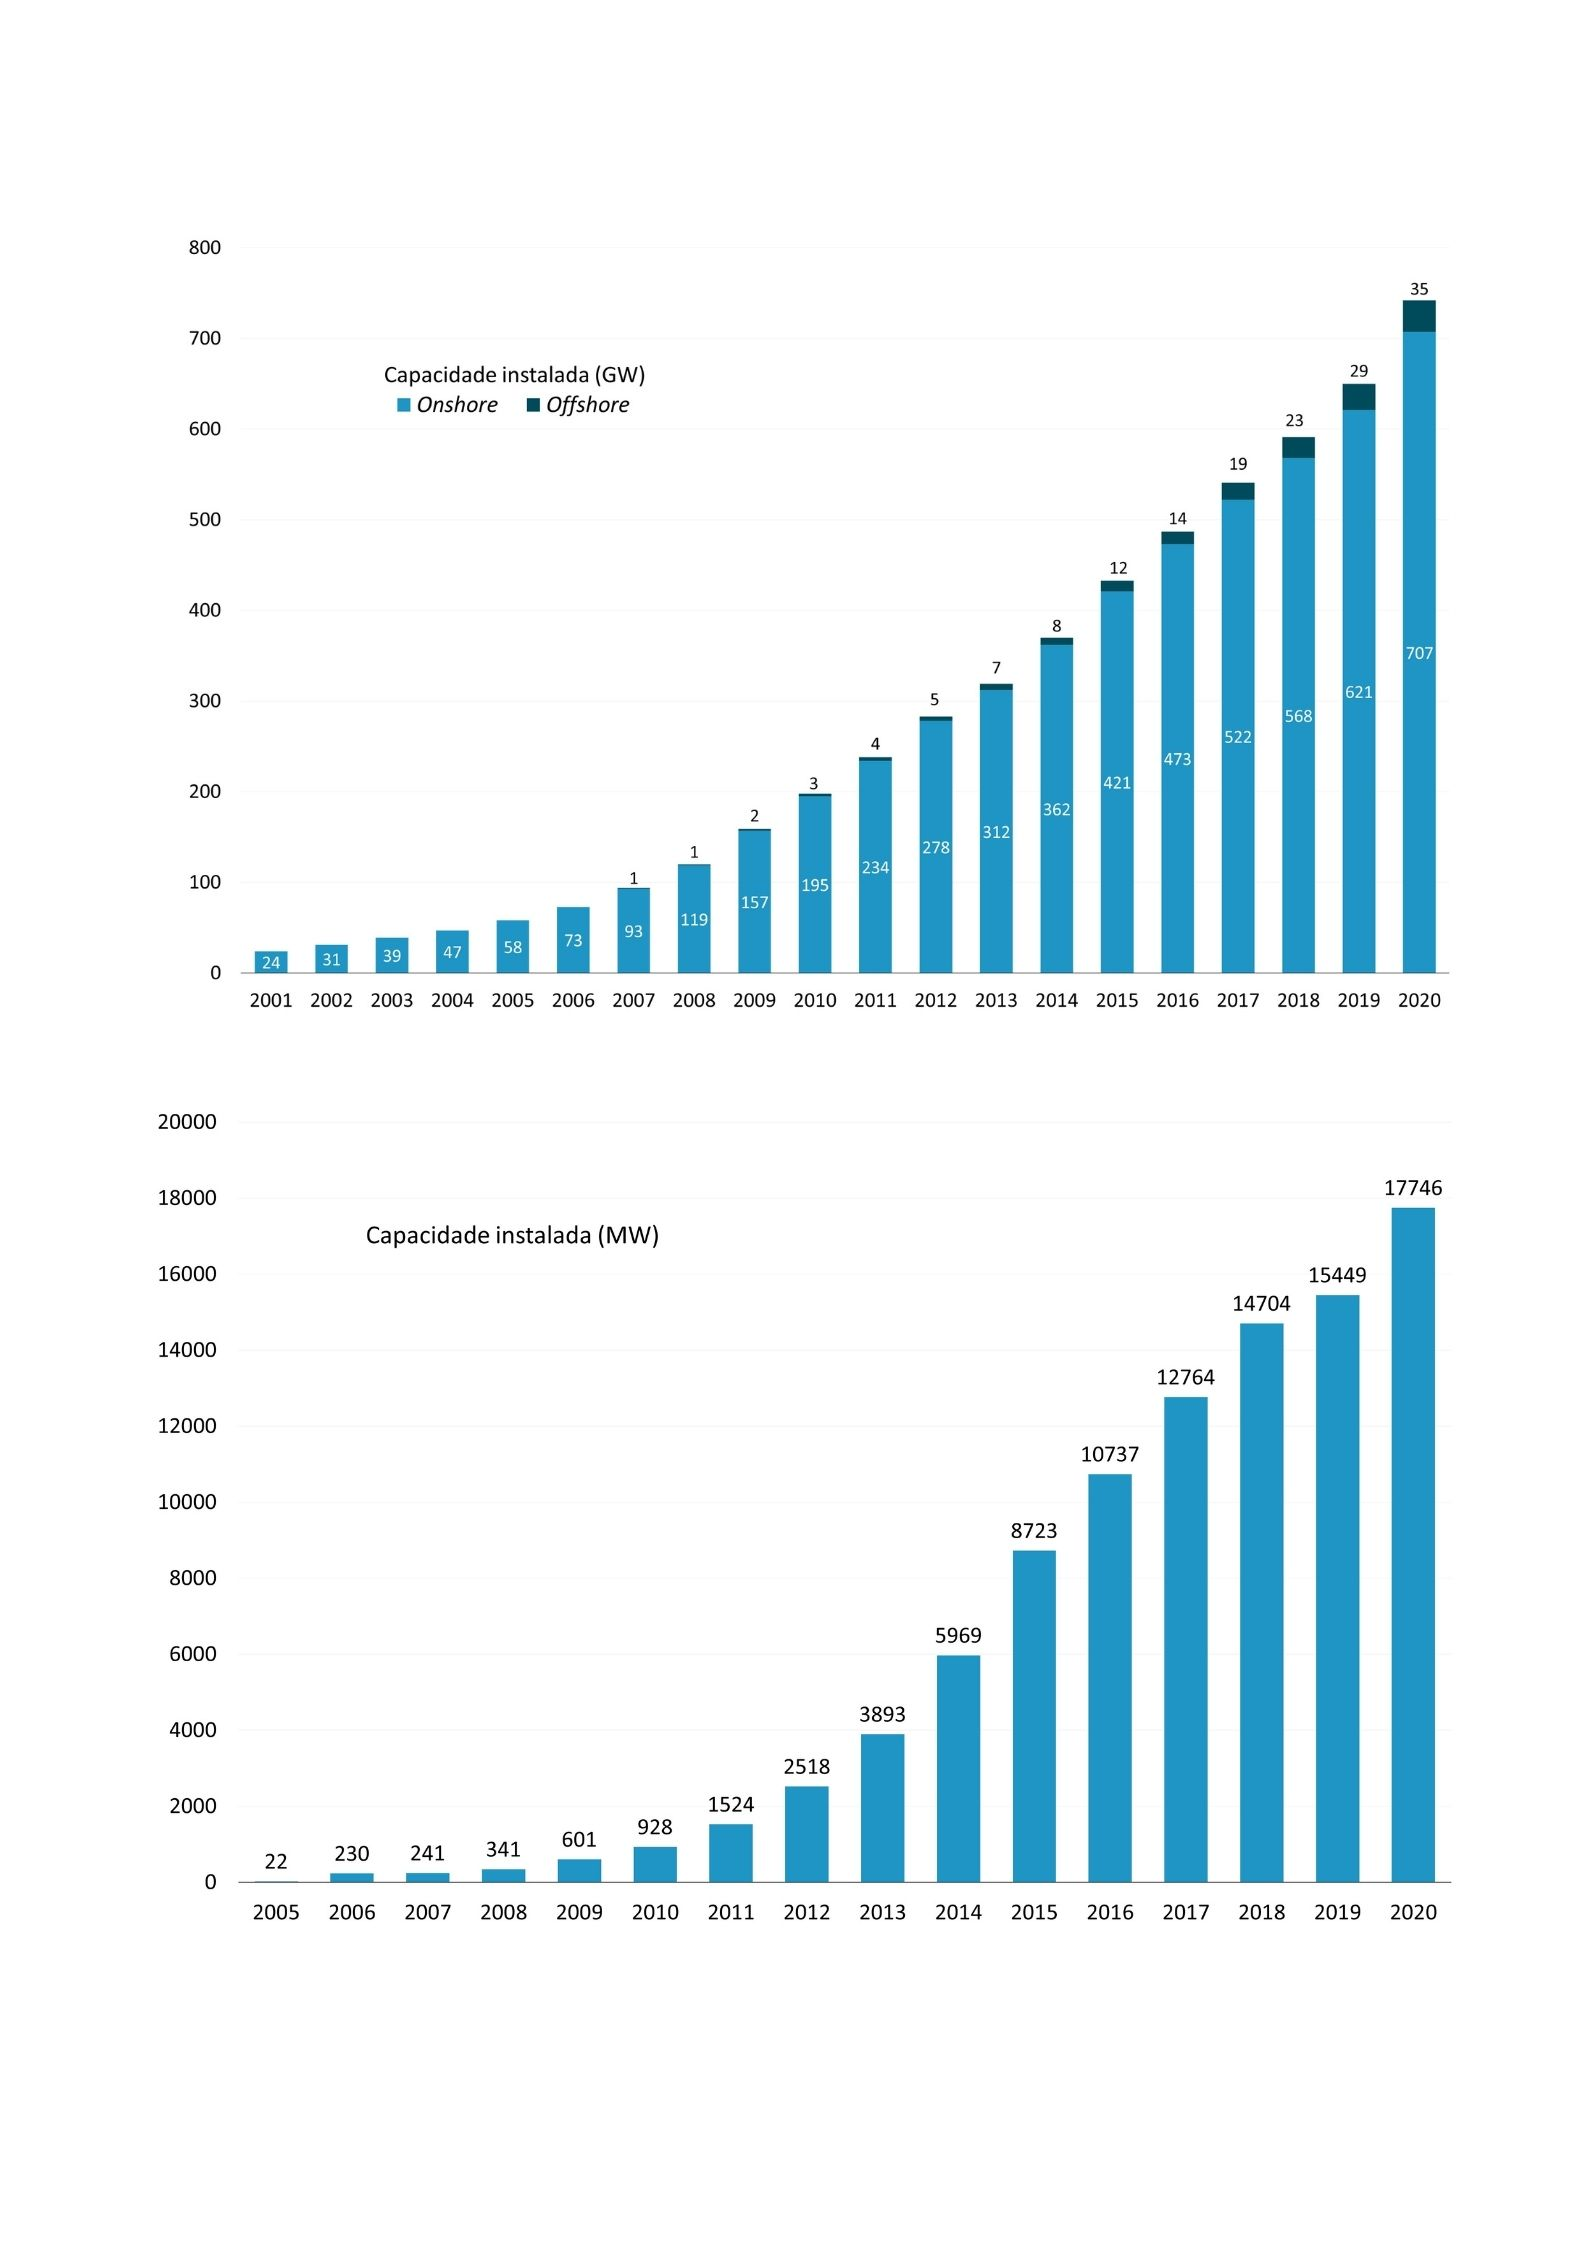
\includegraphics[width=0.9\linewidth]{imagens/cap08/Figura_8.1ab} 

}

\caption{Evolução da capacidade instalada de energia eólica, em terra e no mar, no mundo (em gigawatts GW, acima) (GWEC 2021), e no Brasil, atualmente somente em terra (em megawatts MW, abaixo). Fonte: ABEEólica (2021)}\label{fig:61}
\end{figure}

No Brasil, a partir dos incentivos governamentais instituídos pela Lei nº 10.438/2002 (Programa de Incentivo às Fontes Alternativas de Energia Elétrica -- Proinfa), criou-se um cenário favorável ao desenvolvimento da energia eólica que, de inexpressiva até 2005, já representa cerca de 10\% da matriz elétrica nacional, com um crescimento médio de 36\% ao ano na última década (Figura \ref{fig:62}). Em 2020, a energia eólica respondeu por 10\% da geração injetada no Sistema Interligado Nacional (SIN) e, em dias de pico, representou quase 95\% da energia consumida no subsistema Nordeste (ABEEólica 2021). A totalidade dos parques eólicos instalados no país está em terra, ocupando especialmente o litoral do Nordeste e do extremo Sul do país (Figura 8.2). Nos últimos anos, entretanto, houve uma substancial expansão para o interior, no Estado da Bahia, fazendo com que essa unidade da federação assumisse a co-liderança nacional em capacidade ao lado do Rio Grande do Norte. Cada um desses Estados conta com cerca de 7,5 GW em operação ou construção, em um universo que totaliza 25,1 GW de potência outorgada (ANEEL 2021a) (Figura \ref{fig:63}).

\begin{figure}[H]

{\centering 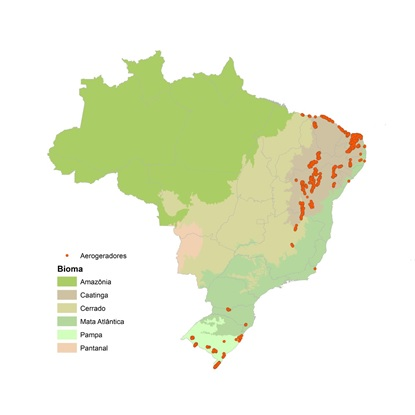
\includegraphics[width=0.55\linewidth]{imagens/cap08/Figura_8.2} 

}

\caption{Localização das usinas eólicas instaladas ou em instalação no Brasil. Fonte: ANEEL (2021b)}\label{fig:62}
\end{figure}

\begin{figure}[H]

{\centering \includegraphics[width=0.65\linewidth]{imagens/cap08/Figura_8.3} 

}

\caption{Usinas eólicas no Brasil: potência outorgada por estado da federação, em operação ou em fase de construção. Fonte: ANEEL (2021a)}\label{fig:63}
\end{figure}

O rápido desenvolvimento da energia eólica \emph{offshore} no mundo, em especial na última década, com perspectiva de reprodução, agora, no Brasil, tem demandado a mobilização de empreendedores, órgãos ambientais e pesquisadores por diretrizes de licenciamento, avaliação de risco e desenvolvimento de metodologias ou abordagens para identificação e mitigação de potenciais impactos, com especial foco nas aves marinhas e costeiras. Esse cenário é bastante desafiador, dada a urgência do tema e a heterogeneidade ambiental e de composição da avifauna ao longo da vasta costa brasileira, para as quais não há uma única e simples abordagem.

Embora alguns dos impactos ambientais decorrentes dos empreendimentos eólicos no mar sejam similares aos terrestres (e.g., impactos por colisão e barreiras aos deslocamentos predominantemente afetando as aves, além de supressão ou alteração de \emph{habitat}), existem outros associados às peculiaridades do ambiente e das espécies marinhas. Por exemplo, enquanto espécies de morcegos frequentemente colidem com estruturas eólicas em ambientes terrestres, a frequência de registros de quirópteros é menor à medida que aumenta a distância da costa (Solick \& Newman 2021). No Brasil, não é conhecido se as espécies de morcegos são migratórias (Bernard \& Delgado-Jaramillo 2019) ou mesmo se ocorrem regularmente em ambiente marinho, onde apenas registros esporádicos (Costa et al.~2006, Esbérard e Moreira 2006, Van Deusen 1961) foram documentados. No mar, as aves marinhas e costeiras são grupos com maior risco, enquanto aves de rapina e Passeriformes, comumente sob elevado risco no ambiente terrestre, devem sofrer pouco ou nenhum impacto em ambientes marinhos. Para as aves marinhas, os riscos são basicamente de mortalidade direta causada por colisão com as estruturas, em especial com as hélices, ou por evitação de habitat anteriormente usados (Furness et al.~2013). Considerando esse problema, o presente capítulo visa:

\begin{enumerate}
\def\labelenumi{\arabic{enumi}.}
\item
  indicar de forma objetiva a legislação aplicável e seu desenvolvimento nos últimos anos, incluindo aquelas normas específicas sobre a tipologia eólica \emph{offshore}, bem como a legislação aplicável às aves marinhas e costeiras;
\item
  fornecer um panorama geral sobre o conhecimento global atual acerca do impacto de eólicas no mar sobre as aves marinhas, identificando as experiências internacionais quanto aos grupos potencialmente impactados e as abordagens de estudo, monitoramento e inovações tecnológicas;
\item
  apontar grupos de aves marinhas de interesse nas áreas de elevado potencial eólico \emph{offshore} no Brasil, dada a demanda de licenciamento atualmente em curso e a ocorrência de espécies conhecidas ou potencialmente ocorrentes nestas áreas;
\item
  apresentar e discutir cuidados importantes a serem levados em conta durante as fases do licenciamento, considerando o conhecimento atual sobre distribuição espacial e comportamento de aves marinhas no Brasil, técnicas e abordagens promissoras para execução do diagnóstico e monitoramento, bem como o balizamento apresentado no Termo de Referência para elaboração de Estudos e Relatórios de Impacto Ambiental -- EIA/RIMAs de Complexos Eólicos \emph{Offshore} (CEO) do IBAMA.
\end{enumerate}

Este texto não tem a pretensão de ser um guia detalhado e definitivo sobre um tema tão complexo e sobre o qual existem muitas lacunas e especificidades. Porém, pretende indicar aspectos gerais que requerem atenção, e fornecer um primeiro cenário da interface entre a energia eólica \emph{offshore} e as aves marinhas e costeiras que ocorrem no Brasil. Sobre o panorama inicial aqui apresentado, futuros direcionamentos e aprimoramentos devem ser aplicados, usando-se uma abordagem adaptativa à medida que avançamos no entendimento sobre o tema e que as atividades são realizadas (\emph{sensu} Bell \& Morse 2003).

\hypertarget{histuxf3rico-no-brasil-e-legislauxe7uxe3o-aplicuxe1vel}{%
\section{Histórico no Brasil e legislação aplicável}\label{histuxf3rico-no-brasil-e-legislauxe7uxe3o-aplicuxe1vel}}

As diversas outras fontes de energia utilizadas no país tiveram o licenciamento realizado de forma corretiva ou sob demanda premente, e verificou-se, posteriormente, que diversos aspectos não haviam sido adequadamente considerados. Diferentemente, a geração de energia a partir da fonte eólica em ambiente marinho tem a rara oportunidade de ser inserida na matriz elétrica brasileira de forma ambiental e estrategicamente planejada.

Apesar de se diferenciar do ambiente terrestre pela ausência de propriedades privadas, o espaço marinho é palco de inúmeros usos e destinações, como exploração de óleo e gás, pesquisa sísmica, cabos e emissários submarinos, dragagens, navegação, pesca artesanal e industrial, turismo, militar, conservação ambiental, entre outros, nem sempre compatíveis entre si. A experiência europeia mostra que um elemento-chave para a redução de impactos ambientais e conflitos de uso é a definição de um Planejamento Espacial Marinho (PEM), instrumento a ser obrigatoriamente elaborado pelos países-membros da União Europeia até 2021, conforme a Diretiva 2014/89/EU. No Brasil, que assumiu o compromisso de implantar o PEM até 2030, como signatário da Conferência da ONU para os Oceanos, de 2017, a Comissão Interministerial para os Recursos do Mar (CIRM) coordena as ações para sua elaboração. Até lá, essa lacuna de planejamento agrega ao processo incertezas e custos desnecessários, pois áreas inadequadas, seja por questões ambientais, seja por incompatibilidade com outras atividades, são objeto de desenvolvimento de projetos que, preliminarmente, poderiam ter sido identificados como inviáveis. Como produto intermediário há a indicação de implantação, pelo governo brasileiro, de um projeto piloto do PEM em uma região do país; seria altamente recomendável que essa iniciativa ocorresse em alguma das regiões de maior potencial eólico (Figura \ref{fig:64}), antecipando, ao menos parcialmente, os benefícios desse instrumento de ordenamento e gestão territorial.

\begin{figure}[H]

{\centering \includegraphics[width=0.75\linewidth]{imagens/cap08/Figura_8.4} 

}

\caption{Potencial eólico no mar ao longo da costa brasileira (World Bank 2019) e localização dos empreendimentos em licenciamento ambiental (IBAMA 2022), detalhados nas três áreas de maior potencial eólico: a) litoral do Nordeste, entre Piauí e Rio Grande do Norte; b) litoral Sudeste, entre o sul do Espírito Santo e o norte do Rio de Janeiro; c) litoral Sul, ao longo da costa central e norte do Rio Grande do Sul.}\label{fig:64}
\end{figure}

Ainda, vislumbra-se um cenário de indefinições regulatórias nos mais diversos aspectos relacionados ao desenvolvimento de um projeto eólico no mar, desde a cessão de uso do território, estabelecimento de prioridades e incompatibilidades de uso, até questões relacionadas aos modelos de outorga e seleção pelo setor elétrico. Já sob o aspecto ambiental propriamente dito, apesar de não haver um instrumento legal específico para a tipologia, o arcabouço legal existente é suficiente para embasar o processo de licenciamento. Os órgãos intervenientes são aqueles regularmente envolvidos no processo de licenciamento ambiental e especificados pela Portaria Interministerial nº 60/2015, consistindo na Fundação Nacional do Índio -- FUNAI, Instituto Nacional de Colonização e Reforma Agrária -- INCRA (originalmente, Fundação Cultural Palmares), Instituto do Patrimônio Histórico e Artístico Nacional -- IPHAN e Ministério da Saúde. Quando o empreendimento afetar Unidade de Conservação (UC), conforme previsão da Lei Federal nº 9.985/2000 e Resolução CONAMA nº 428/2010, deverá ser solicitada autorização do órgão responsável por sua administração. No caso de UCs federais, esse órgão é o ICMBio e os procedimentos relativos à sua autorização para licenciamento ambiental estão previstos na Instrução Normativa Conjunta ICMBio/IBAMA nº 8/2019. Essa IN também faculta ao IBAMA solicitar manifestação técnica especializada do ICMBio acerca de eventuais impactos sobre espécies ameaçadas de extinção, a qual terá caráter opinativo e não vinculante, assim como determina que sejam observados os Planos de Ação Nacional e as áreas geográficas de concentração de espécies ameaçadas. No caso de captura e marcação de aves silvestres durante os estudos prévios visando o licenciamento ou o monitoramento durante as fases de instalação e operação, é necessário obter também autorizações no Sistema Nacional de Anilhamento, gerido pelo ICMBio/CEMAVE (IN GABIN/ICMBIO nº 7/2021). Além disso, a IN ICMBio/IBAMA nº 01/2014 determina que os dados relativos à fauna silvestre oriundos dos estudos, programas de monitoramento e procedimentos de resgate de fauna vinculados ao licenciamento ambiental federal sejam depositados em banco de dados com acesso amplo e irrestrito de ambos os órgãos. Nesse sentido, encontra-se em fase de desenvolvimento a plataforma SISBIA (Sistema de Gestão de Dados de Biodiversidade para Avaliação de Impacto Ambiental), que também prevê nível público de acesso.

Deve-se destacar a definição de competência da União para promover o licenciamento ambiental dos empreendimentos ou atividades localizados ou desenvolvidos no mar territorial, na plataforma continental ou na Zona Econômica Exclusiva, conforme o Art. 7º, XIV, b, da Lei Complementar nº 140/2011, e especificamente das usinas eólicas, no caso de empreendimentos e atividades \emph{offshore} e zona de transição terra-mar, como posteriormente regulamentado pelo Art. 3º, VIII, c, do Decreto Federal nº 8.437/2015. Com a exclusividade de competência atribuída ao ente federal, supera-se de imediato a indesejável discrepância entre os graus de complexidade dos estudos ambientais exigidos pelos diferentes estados, fato observado, em particular, na primeira década de desenvolvimento das usinas eólicas em terra, num contexto de disputa pela atração de investimentos. Fundamentando-se na Resolução CONAMA nº 279/2001, que prevê procedimento simplificado para o licenciamento ambiental de empreendimentos com pequeno impacto ambiental, usinas eólicas foram, por vezes, licenciadas com estudos superficiais, ainda que localizadas em áreas sensíveis ou sendo projetos de grande porte. Tais divergências e os consequentes riscos derivados das insuficientes avaliações de impacto ambiental foram propulsores da elaboração da Resolução CONAMA nº 462/2014, que estabeleceu critérios para enquadramento dos projetos quanto ao potencial de impacto e consequente rito de licenciamento, inclusive fornecendo o conteúdo mínimo dos diferentes tipos de estudo ambiental.

Diante da ausência de normativa similar para usinas eólicas \emph{offshore} e prevendo a iminente proposição de projetos, o IBAMA definiu uma agenda para capacitação do corpo técnico e elaboração de quadro normativo. Já em 2015, no desenvolvimento das matrizes de impacto por tipologias, o Instituto realizou uma primeira identificação das atividades, aspectos, impactos e medidas mitigadoras inerentes aos empreendimentos eólicos marítimos, a partir da bibliografia existente. Posteriormente, em parceria com o programa ``Diálogos Setoriais'', da União Europeia, realizou encontros com especialistas nacionais e internacionais em 2019, bem como produziu estudo sintetizando a experiência e comparando as práticas adotadas em países pioneiros na implantação de empreendimentos eólicos \emph{offshore} (Vasconcelos 2019). Com isso, reuniu-se informação suficiente para propor um Termo de Referência (TR) Padrão para Estudo de Impacto Ambiental e Relatório de Impacto Ambiental (EIA/RIMA) de Complexos Eólicos Marítimos (IBAMA 2020), submetido à consulta pública e lançado, em sua versão final, em novembro de 2020. Entre as próximas metas da agenda do órgão licenciador federal estão a elaboração de um Guia de Avaliação de Impacto para a tipologia e norma específica para disciplinar seu licenciamento.

O termo de referência apresenta o escopo e encadeamento lógico a serem observados no estudo de impacto ambiental necessário à avaliação de viabilidade de cada projeto. Conforme a estimativa prévia de intensidade dos impactos, maior ênfase foi direcionada a aspectos relacionados aos usos potencialmente conflitantes (por exemplo, óleo e gás, pesca, navegação, turismo), interferências paisagísticas e infraestrutura necessária (porto de apoio). O diagnóstico do meio biótico remete para uma maior complexidade no que se refere aos grupos tartarugas, aves e mamíferos marinhos, bem como aos ambientes recifais. Embora preservando certo grau de autonomia aos consultores, o TR indica uma ou mais alternativas metodológicas para obtenção de dados, conforme as melhores práticas internacionais e o estado da arte no momento de sua elaboração, sem restringir a proposição de métodos alternativos nos planos de trabalho de cada projeto individual.

A definição do tipo de estudo exigido e de seu escopo, apresentada no termo de referência, traz segurança ao processo, possibilidade de planejamento prévio pelo empreendedor e isonomia entre os proponentes. Ressalta-se que, apesar de ser um TR padrão para a tipologia, é prevista sua adaptação às particularidades do projeto e da região onde se insere. Além disso, para projetos experimentais, com até duas turbinas ou instalados sobre plataformas já existentes, podem ser aplicáveis estudos ambientais simplificados. O significativo aumento no número de processos em licenciamento pode ser um reflexo da relevância da definição de procedimentos claros. Se entre 2016, ano de instauração do primeiro processo, a novembro de 2020, mês de lançamento do TR, apenas 11 processos haviam sido abertos, desde então 38 novos projetos já foram apresentados.

Analisando-se sua distribuição espacial, constata-se, como esperado, a atração pelas três regiões com maior potencial eólico ao longo da costa brasileira: litoral do Nordeste, do Piauí ao Rio Grande do Norte; litoral Sudeste, do Rio de Janeiro ao Espírito Santo; e litoral Sul, em especial, no Rio Grande do Sul (Figura 8.4). O afastamento médio da costa é de cerca de 14 km e as configurações propostas apresentam aerogeradores com potência de 12 a 15 MW, torres de 150 m e pás de 120 m em média, resultando em alturas máximas de aproximadamente 270 m. A princípio, dadas as profundidades tipicamente inferiores a 50 m, todos os parques preveem fundações do tipo \emph{monopile}, com estacas cravadas no solo marinho. Essas estruturas são de instalação mais fácil e menores custos, razões pelas quais são as mais utilizadas nessa faixa de profundidade globalmente (Hernandez-C et al.~2021) (Figura \ref{fig:65}).

\begin{figure}[H]

{\centering \includegraphics[width=0.75\linewidth]{imagens/cap08/Figura_8.5} 

}

\caption{Tipos de estrutura de fixação de turbinas eólicas \emph{offshore}. A - Monopés ou estacas (\emph{Monopile}), B - Base gravitacional (\emph{Gravity base}) e C - Tripés (\emph{Jacket and tripods}). Imagem: Manzano-Agugliaro et al.~(2020) {[}CC BY{]}}\label{fig:65}
\end{figure}



A busca por áreas com maior potencial eólico e menor profundidade, bem como a proximidade com infraestrutura portuária consolidada, fizeram com que começassem a surgir sobreposições de poligonais projetadas para diferentes empreendimentos. Como subsídio aos empreendedores, desde junho de 2021 o IBAMA disponibiliza publicamente um \href{https://www.ibama.gov.br/laf/consultas/mapas-de-projetos-em-licenciamento-complexos-eolicos-offshore}{mapa dos empreendimentos em licenciamento}, atualizado sempre que um novo processo é iniciado ou finalizado. Desde então, nenhuma nova sobreposição foi verificada, apontando para a importância da transparência e publicidade de informações que auxiliem na elaboração dos projetos, sendo esse princípio igualmente aplicável às informações ambientais geradas nos estudos e monitoramentos exigidos durante o licenciamento. No entanto, a demanda por instalação de diferentes empreendimentos em áreas adjacentes, gera uma barreira contínua ao longo da costa, com implicações para a navegação e potencial surgimento de barreiras para organismos marinhos. Esse aspecto suscita preocupações quanto aos efeitos cumulativos, em nível de populações (e.g., Goodale \& Milman 2020), comunidades ou guildas de aves (Goodale et al.~2019). Em especial, os impactos são maiores nas populações de aves que usam a região nerítica (Goodale et al.~2019), devendo ser abordados com cautela e olhar em macroescala.

Em relação ao marco legal relacionado, especificamente, a estratégias para a conservação das aves marinhas e costeiras no Brasil, que potencialmente podem interagir com CEOs, merecem destaque os Planos de Ação Nacional para a Conservação de Espécies Ameaçadas (PANs). Os PANs definem ações \emph{in situ} e \emph{ex situ} para a conservação e recuperação de espécies. São instrumentos de implementação da Política Nacional da Biodiversidade, contemplados pela Portaria MMA n° 43, de 31 de janeiro de 2014, que institui o Programa Nacional de Conservação das Espécies Ameaçadas de Extinção -- Pró-Espécies. Os PANs geridos pelo ICMBio são regulamentados pela IN ICMBio nº 21, de 18 de dezembro de 2018, que disciplina os procedimentos para sua elaboração, aprovação, publicação, implementação, monitoria, avaliação e revisão. Os planos de ação contemplando espécies da Classe Aves com maior interface com CEOs incluem o PAN Albatrozes e Petréis -- PLANACAP (Portaria ICMBio nº 378, de 24 de abril de 2018), o PAN Aves Marinhas (Portaria ICMBio nº 286, de 4 de abril de 2018), e o PAN Aves Limícolas Migratórias (Portaria ICMBio nº 491, de 10 de setembro de 2019).

Além disso, uma vez que muitas das espécies de aves marinhas migratórias ameaçadas que utilizam águas brasileiras usam territórios de outros países para completar seus ciclos de vida, a participação consolidada do Brasil no Acordo Internacional para a Conservação dos Albatrozes e Petréis -- ACAP, e como membro do Conselho Científico e parte da Convenção sobre a Conservação das Espécies Migratórias de Animais Silvestres -- CMS das Nações Unidas tem, principalmente na última década, reforçado essa importante rede de colaboração para fortalecer e qualificar estratégias de conservação dessas espécies. O engajamento nacional nessas estratégias compartilhadas entre países é respaldado legalmente no Brasil por instrumentos como o Decreto nº 6.753/2009, que promulga o Acordo para a Conservação de Albatrozes e Petréis, adotado na Cidade do Cabo, em 2 de fevereiro de 2001; o Decreto Legislativo nº 387 de 15 de outubro de 2013, que aprova o texto da Convenção sobre a Conservação das Espécies Migratórias de Animais Silvestres, assinado em Bonn, em 23 de junho de 1979; e o Decreto nº 9.080/2017, que promulga a CMS no país, tornando o Brasil uma de suas nações parte.

\hypertarget{euxf3licas-offshore-e-potenciais-efeitos-sobre-as-aves-marinhas-e-costeiras}{%
\section{\texorpdfstring{Eólicas \emph{offshore} e potenciais efeitos sobre as aves marinhas e costeiras}{Eólicas offshore e potenciais efeitos sobre as aves marinhas e costeiras}}\label{euxf3licas-offshore-e-potenciais-efeitos-sobre-as-aves-marinhas-e-costeiras}}

O conhecimento atual sobre os efeitos de eólicas \emph{offshore} concentra-se em iniciativas de pesquisa e monitoramento desenvolvidas no hemisfério Norte. Tais efeitos são muito variáveis em função da qualidade do \emph{habitat}, da distribuição de presas, da configuração do complexo eólico e de sua localização em relação às áreas reprodutivas e de alimentação das espécies (Bennun et al.~2021a).

Os impactos dos CEOs sobre as aves marinhas e costeiras podem ser, basicamente, de dois tipos: 1) por colisão, quando a ave falha em evitar os aerogeradores, sendo identificado pela ocorrência de aves mortas ou lesionadas no entorno das turbinas, especialmente aplicável a turbinas eólicas \emph{onshore}, mas potencialmente identificável através de carcaças encontradas nas praias, ou no mar, com câmeras tradicionais ou termais (para uso noturno ou sob neblina); e 2) por realocação ou deslocamento (do inglês \emph{displacement}), quando as aves evitam a área do empreendimento e, consequentemente, deixam de usar o local para suas atividades básicas. Na prática, com a instalação dos CEOs há a criação de áreas de exclusão ou alteração de \emph{habitat} utilizados pelas aves, sejam áreas de alimentação (Welcker \& Nehls 2016), interrupção de corredores de deslocamento causando um efeito barreira (Cook et al.~2014) ou gerando maior gasto energético em função da alteração de rotas, ou alterações na estrutura dos ecossistemas, incluindo mudanças nas relações tróficas (Perrow 2019). A evitação da área, segundo Furness et al.~(2013), pode ocorrer em macroescala, quando todo o CEO é evitado, ou em microescala, quando a área segue em uso, mas o comportamento para desviar das turbinas é realizado pelas aves. O comportamento em nível do interior do empreendimento é referido como de mesoescala por Thaxter et al.~(2018). Adicionalmente, a realocação pode ser por atração, na qual as aves são atraídas para as áreas dos CEOs, em especial para uso das estruturas como locais de pouso e descanso (Vanermen et al.~2015, Dierschke et al.~2016).

Os impactos diretos de estruturas eólicas \emph{offshore} sobre as aves marinhas têm sido inferidos principalmente através de estudos teóricos que abordam impactos potenciais. Essa tendência decorre do fato da identificação empírica de indivíduos afetados por eventos de colisão ser logisticamente difícil (Bennum et al.~2021b). Da mesma forma, a inferência sobre impactos por mudança de área de uso, por realocação, pode diferir entre espécies similares ou entre populações, e requer dados referentes aos padrões pré-instalação para uma avaliação acurada dos efeitos oriundos dos CEOs, uma vez instalados. Portanto, os estudos prévios têm um papel fundamental na avaliação de risco desses empreendimentos e na proposição de medidas de mitigação de seus impactos ambientais. Igualmente relevante é a obtenção de dados sobre uso do espaço, comportamento e rotas de deslocamento das aves, como subsídios ao entendimento mecanístico de mudanças de padrões que possam ser detectadas em comparações pós-instalação (e.g., Petersen et al.~2011).

A redução ou interrupção no uso, pelas aves, da área utilizada para instalação do empreendimento pode representar alterações de áreas de forrageio e descanso (Welcker \& Nehls 2016) e redefinição de suas trajetórias de voo (i.e., efeito barreira; Masden et al.~2009, 2010). Tais consequências podem ser observadas pela diferença no uso da área entre os períodos anterior e posterior à instalação do empreendimento; também, após a instalação, entre a área interna e externa do empreendimento (evitação em macroescala; Desholm \& Kahlert 2005). Alternativamente, as aves podem seguir utilizando ou, até mesmo, serem atraídas para a área do empreendimento após a instalação dos aerogeradores. Por exemplo, as estruturas eólicas podem fornecer locais para pouso, em especial para biguás (Dierschke et al.~2016) ou propiciar melhores condições para alimentação para espécies piscívoras (Vanermen et al.~2015, Degraer et al.~2020). Os complexos podem, ainda funcionar como elementos da paisagem, utilizados para a orientação durante o voo noturno (Vasconcelos 2019) ou aumentar a disponibilidade de alimento, uma vez que há restrições a embarcações pesqueiras 500 m no entorno da poligonal licenciada, conforme NORMAM-11/DPC, de 2017, da Marinha do Brasil. Ainda, as estruturas construídas podem agir como recifes artificiais, atraindo presas potenciais (Langhamer 2012, Bergström et al.~2013). Perrow (2019) sugere que mudanças de comportamento das aves na área do empreendimento possuem implicações espécie-específicas para o desempenho e gasto energético individuais, sendo as aves mergulhadoras as mais sensíveis. Desse modo, o uso do espaço por aves marinhas no interior e no entorno do empreendimento precisa ser avaliado antes e após a instalação dos aerogeradores.

Os aerogeradores \emph{offshore} são fixados por meio de tecnologias distintas, implicando em diferentes impactos associados à sua instalação. As tecnologias mais utilizadas são as fundações fixadas diretamente no leito marinho, dentre as quais a do tipo \emph{monopile} é o modelo tipicamente empregado em profundidades de até 60 m (Bennun et al.~2021a). Ruídos extremamente elevados são produzidos durante sua instalação, devido à percussão no fundo do mar. Presume-se que a tecnologia de aerogeradores flutuantes, na qual a torre localiza-se sobre uma plataforma ancorada ao fundo do mar por cabos, resulte em menos ruídos durante a instalação, caso não sejam igualmente utilizadas estacas no sistema de ancoragem. Além disso, a opção por aerogeradores flutuantes tem a vantagem de viabilizar a implantação de complexos eólicos em maiores profundidades. Conforme o tipo de fundação ou ancoragem, são formados substratos em extensões variáveis, que funcionam como recifes submersos artificiais, compondo um novo \emph{habitat}.

Além do impacto individual de cada turbina instalada e de seu conjunto, é importante observar que as estruturas associadas incluem subestações e cabos submarinos, instalações na costa adjacente que dão suporte às instalações \emph{offshore}, tais como subestações terrestres, cabos subterrâneos e linhas de transmissão. O conjunto dessas estruturas, seus efeitos cumulativos regionais e seus impactos sobre a biodiversidade e funcionamento ecossistêmico devem ser sempre considerados em qualquer análise de impacto (e.g., Raoux et al.~2018).

Há evidências de que as gaivotas (Laridae) são as espécies de aves marinhas mais frequentemente impactadas por colisão em parques eólicos \emph{offshore}, seguidas por espécies de trinta-réis (Sterninae), no caso de aerogeradores instalados mais próximos da costa (Skov et al.~2018, King 2019). O principal fator preditivo, no caso das fatalidades regulares por colisão com aerogeradores \emph{offshore} relatadas para gaivotas, foi o tempo despendido pela ave na altitude do rotor (Skov et al.~2018). Quanto aos componentes costeiros dos parques eólicos \emph{offshore}, as linhas de transmissão, subestação terrestre e estruturas associadas podem impactar espécies com alta carga alar (massa corporal em relação à área de asa), como algumas aves de rapina e cisnes. Tais grupos podem estar particularmente sujeitos a maiores riscos, advindos da colisão com linhas de transmissão associadas ao empreendimento. Em determinadas situações, os impactos por evitação e colisão podem estar associados, como demonstrado para Anseriformes, que evitam toda a área durante o dia, provavelmente porque a detectam visualmente, mas usam o espaço dos CEOs à noite, por exemplo durante migrações, quando então há aumento dos riscos de colisão (Desholm \& Kahlert 2005).

Algumas aves limícolas (ordem Charadriiformes) e aves aquáticas (por exemplo, Anseriformes) realizam voos em mar aberto durante suas migrações e são registradas durante o monitoramento em plataformas \emph{offshore} e por radares em alguns locais do mundo, com altitudes de voo variando consideravelmente, mas em geral, a menos de 200 m de altitude (Alves et al.~2016, Conklin et al.~2017, Hüppop et al.~2019). No entanto, para a América do Sul, há poucas informações sobre detalhes do comportamento migratório da maioria das espécies (Hernandez-C. et al.~2021). A ausência de Anseriformes marinhos no Brasil, comuns em áreas temperadas frias do hemisfério Norte e também no sul da América do Sul, demonstra uma diferença importante na composição da avifauna em águas marinhas rasas. Por outro lado, entre as aves limícolas migratórias ocorrentes no Brasil existem espécies em grande risco de extinção, devido à perda de \emph{habitat} ao longo de suas rotas de migração. Impactos adicionais advindos de geração de energia eólica podem, potencialmente, gerar efeitos catastróficos em populações deste grupo, notadamente nas áreas de maior agregação ao redor do mundo (Melville et al.~2016).

\hypertarget{as-aves-marinhas-e-costeiras-no-brasil}{%
\section{As aves marinhas e costeiras no Brasil}\label{as-aves-marinhas-e-costeiras-no-brasil}}

A extensão latitudinal de cerca de 38º ao longo da costa brasileira oferece variadas condições ambientais para o grupo das aves marinhas, o que sustenta uma assembleia que representa cerca de um terço (\textasciitilde100 espécies) das cerca de 350 espécies de aves marinhas existentes no mundo. Uma fração substancial desse total é composta por aves de ocorrência ocasional, usualmente denominadas vagantes (Pacheco et al.~2021) e que são, portanto, de menor relevância no contexto das eólicas \emph{offshore}. A heterogeneidade da paisagem marinha ao longo da extensa costa atende aos requerimentos de espécies tipicamente tropicais, em sua porção norte, e de espécies temperadas e antárticas, em sua porção sul. A Zona Econômica Exclusiva brasileira representa área de invernagem para migrantes austrais e boreais, e ainda, de reprodução e alimentação para espécies residentes, as quais utilizam ilhas em regiões neríticas (sobre a plataforma, em especial, próximo à costa) e oceânicas para nidificação.

A classificação das espécies como residentes ou migratórias (i.e., que se reproduzem em território brasileiro e realizam deslocamentos cíclicos) é relevante para a avaliação de impacto de CEOs. Essa classificação pode, por exemplo, ajudar a definir locais de agregação naturais, com deslocamentos regulares entre as colônias e as áreas de alimentação, ou movimentos mais livres, sem a necessidade de retorno regular a um ponto. Neste contexto, é possível identificar algumas das ilhas oceânicas como de menor relevância em relação aos empreendimentos eólicos em processo de licenciamento atualmente que, quase em sua totalidade, restringem-se a profundidades inferiores a 50 m nas três áreas de interesse primário citadas acima (Figura 8.4). Assim, a Ilha da Trindade, o Arquipélago de São Pedro e São Paulo e, possivelmente, o Arquipélago de Fernando de Noronha, são de menor relevância neste momento. No entanto, as aves que se reproduzem no Atol das Rocas, em especial aquelas que tendem a deslocar-se em direção à costa, como \emph{Sula leucogaster}, demandam especial atenção, pois podem atingir as áreas onde já há pedidos de licenciamento, como ao longo da costa do Rio Grande do Norte e estados próximos. Por exemplo, sabe-se que \emph{Pterodroma arminjoniana} usa a costa brasileira durante parte do seu período reprodutivo (Leal \& Bugoni 2021) ou utiliza as costas Norte e Nordeste brasileiras, incluindo Piauí, Ceará e Rio Grande do Norte, durante sua migração entre o Atlântico Norte e as colônias em Trindade (Leal \& Bugoni 2021). Por outro lado, rastreamento de \emph{S. dactylatra} fora do período reprodutivo em Fernando de Noronha indica que esta espécie não se dirige regularmente em direção à costa, mesmo durante o período não reprodutivo (Roy et al.~2021). Adicionalmente, havendo empreendimentos no sul da Bahia e Espírito Santo, as aves de Abrolhos passam a merecer especial atenção, pois podem atingir áreas costeiras durante suas viagens de alimentação (Nunes et al.~2022). O mesmo aplica-se às espécies que se reproduzem em ilhas costeiras próximas aos locais de interesse, como por exemplo as ilhas da região norte do Rio de Janeiro e do litoral de Santa Catarina, onde \emph{S. leucogaster} e \emph{Fregata magnificens} se reproduzem (Alves et al.~2004) e há elevado potencial eólico.

A ampla maioria das aves marinhas migratórias que ocorrem no Brasil são oriundas da região antártica e subantártica, Patagônia, ilhas e costas do Atlântico Sul, mas também da Nova Zelândia e Austrália. Uma parcela menor é composta pelos migrantes boreais (Tabela 8.1), provenientes da América do Norte, Europa e ilhas da Macaronésia. A origem biogeográfica das espécies é um aspecto relevante, pois pode determinar a sazonalidade de sua presença nas águas brasileiras e, assim, influenciar o desenho amostral nas fases de diagnóstico e monitoramento. Por exemplo, migrantes austrais ocorrem no Brasil, predominantemente, do final do outono a meados da primavera. Um número menor de espécies se reproduz em território brasileiro, em ilhas oceânicas, como São Pedro e São Paulo, Atol das Rocas, Fernando de Noronha, Ilha da Trindade e Martin Vaz, além de Abrolhos, que embora contenha espécies tipicamente oceânicas, está localizada sobre a plataforma continental (Mancini et al.~2016). Adicionalmente, diversas espécies, como gaivotas e trinta-réis, se reproduzem em ilhas costeiras, de Santa Catarina ao litoral do Espírito Santo, sendo que algumas também se reproduzem nas ilhas oceânicas, tais como atobás e fragatas (Branco 2004).

Por sua vez, as aves limícolas que utilizam a região costeira, incluindo praias arenosas, planícies de maré, manguezais, estuários e lagoas costeiras (excetuando, nessa abordagem, as limícolas continentais - Tabela 8.1), distribuem-se de Norte a Sul do país. No entanto, há áreas de agregação importantes de aves limícolas no litoral do Rio Grande do Sul, bem como ao longo de parte dos litorais Sudeste, Nordeste e Norte. Esses grupos utilizam a Rota Atlântica para migração, quando supostamente deslocam-se em grandes altitudes, da ordem de centenas a milhares de metros sobre o nível do mar. Porém, nos deslocamentos menores nas áreas não reprodutivas brasileiras, as aves limícolas podem cruzar extensões do oceano voando em altitudes mais baixas, na faixa de ação das hélices dos aerogeradores. Como as áreas com elevado potencial de geração de energia eólica \emph{offshore} estão distribuídas ao longo de toda a costa e contemplam as regiões Sul, Sudeste e Nordeste, é possível identificar grupos de aves marinhas e costeiras que podem apresentar elevada vulnerabilidade à presença dos aerogeradores em cada região e que, portanto, devem ser contempladas nas fases de diagnóstico e monitoramento de CEOs.

A região Sul do Brasil, em especial a costa do Rio Grande do Sul e a porção sul da costa catarinense, possuem marcada sazonalidade em relação à dinâmica oceanográfica, o que tem como consequência uma variação temporal na composição da assembleia de aves marinhas que utiliza a região. A ocorrência de uma frente subtropical de plataforma na região, influenciada pelas águas de plataforma subantártica, tropical e pela pluma de água doce do Rio da Prata, elevam a produtividade primária e atraem espécies que utilizam as áreas visadas pelos CEOs, para alimentação ou como corredor de deslocamento. Entre os migrantes austrais que ocorrem nas áreas com batimetria de até 50 m destacam-se \emph{Procellaria aequinoctialis} e \emph{Thalassarche chlororhynchos}, espécies que se encontram ameaçadas globalmente de extinção devido a uma série de ameaças no mar e nas áreas reprodutivas, como a captura incidental em pescarias, a poluição marinha e a predação de ninhos por espécies exóticas (BirdLife International 2018). O albatroz \emph{T. chlororhynchos} é o que se encontra mais ameaçado por impactos antrópicos e apresenta tendência de declínio populacional. Além de estar categorizado como ``Em Perigo'' (EN), utiliza a área de potencial eólico \emph{offshore} do Sul e Sudeste do Brasil também durante o período reprodutivo, quando está com ninhos ativos em Tristão da Cunha (Gabani 2020). Por fim, há de se destacar espécies que realizam extensos deslocamentos entre as colônias e as áreas de alimentação, quando podem atingir as águas territoriais brasileiras, como é o caso de \emph{Diomedea exulans} e \emph{P. conspicillata}, que chegam ao sul do Brasil, mas permanecem em águas profundas da plataforma externa e talude (Bugoni et al.~2009, Carneiro et al.~2020).

Adicionalmente, a região Sul, de interesse para instalação de CEOs, é amplamente utilizada por espécies de gaivotas e trinta-réis (Laridae), as quais se reproduzem em ilhas costeiras do sul do Brasil, Uruguai, Argentina e Estados Unidos, a exemplo de \emph{Sterna hirundinacea} (ameaçada de extinção no Brasil), \emph{S. hirundo}, \emph{Thalasseus acuflavidus}, \emph{T. maximus} (as duas últimas ameaçadas de extinção no Rio Grande do Sul e \emph{T. maximus}, ameaçada nacionalmente) e \emph{Larus dominicanus}. Durante o período não reprodutivo, tais espécies utilizam a costa sul do Brasil para alimentação, a qual se dá na superfície da coluna d'água, em áreas de baixa profundidade, e envolve movimentos diários cíclicos entre as áreas de alimentação, no mar, e de descanso, durante o dia, ou dormitório noturno, no cordão litorâneo (e.g., Bugoni \& Vooren 2005, Bugoni et al.~2005). Portanto, projetos de instalação de CEOs ao longo da costa sul do Brasil deveriam dedicar atenção, nas fases de diagnóstico e monitoramento, para espécies de Procellariiformes e Charadriiformes que utilizam a região, incluindo espécies bentívoras que se alimentam ao longo das praias arenosas e áreas úmidas costeiras (ver abaixo).

A região Sudeste, em especial as porções norte do Rio de Janeiro e sul do Espírito Santo, são de especial interesse pelos ventos adequados à produção de energia e proximidade aos mercados consumidores dessa energia produzida (Figura 8.4). Porém, esses locais apresentam flutuação sazonal nas condições ambientais, pois possuem forte influência do vento nordeste que faz ressurgir a Água Central do Atlântico Sul e, consequentemente, elevar a produtividade primária na região. Além de abrigar espécies de trinta-réis que se reproduzem e se alimentam na região e adjacências, como \emph{S. hirundinacea}, \emph{T. maximus} e \emph{T. acuflavidus}, as áreas com potencial eólico \emph{offshore} também são utilizadas por espécies de Suliformes, como \emph{S. leucogaster} e \emph{F. magnificens}. Os atobás, incluindo \emph{S. leucogaster}, obtêm o alimento através do mergulho denominado \emph{plunge-diving}, no qual a ave se lança em queda livre a partir de uma determinada altitude para capturar a presa na subsuperfície da coluna d'água. O momento anterior à descida é caracterizado por ganho de altitude, velocidade reduzida e aumento das frequências de mudança de rumo, com patrulhamento da superfície em círculos (Nelson 2005), o que pode representar um aumento da vulnerabilidade dessas espécies ao impacto com as pás dos aerogeradores durante o comportamento de alimentação. Adicionalmente, parte da dieta de \emph{S. leucogaster} é composta por descartes da pesca de arrasto na plataforma continental brasileira e, especificamente, na região Sudeste do Brasil (Souza 2021) e poderia ser influenciada, positiva ou negativamente, com a implementação de uma zona de exclusão de pesca na área do empreendimento e adjacências. É possível que, de forma similar a outros Sulidae do hemisfério Norte (e.g., Goodale \& Milman 2020), os atobás no Brasil também estejam ameaçados por empreendimentos eólicos. O voo planado e o cleptoparasitismo (roubo de alimento de outros indivíduos) de \emph{F. magnificens} também podem elevar a vulnerabilidade da espécie, pois o primeiro ocorre em baixas velocidades, com frequente mudança de rumo, e inclui até mesmo momentos de baixa atividade cerebral na fase de ascensão (Rattenborg et al.~2016), e o segundo está associado a uma queda em alta velocidade e perseguição de outras aves, como \emph{S. leucogaster}. A velocidade de voo pode ser um componente importante na definição de riscos, sendo bastante variável entre áreas e períodos (Masden et al.~2021). Embora escassos, os dados de altitude de voo de fragatas indicam substancial uso das faixas de altitude coincidentes com o rotor de turbinas eólicas, com cerca de 50\% do tempo despendido em voo entre 100 e 200 m (Clark et al.~2020). Por fim, cabe destacar que as áreas da região Sudeste com potencial eólico \emph{offshore} também são utilizadas por \emph{T. chlororhynchos} durante os períodos não reprodutivo e reprodutivo, com uso particularmente intenso da região sob influência da ressurgência de Cabo Frio, conforme demonstrado através de rastreamento remoto de animais no Oceano Atlântico sudoeste (Gabani 2020).

A região Nordeste com elevado potencial eólico \emph{offshore} apresenta maior amplitude longitudinal de áreas propícias aos CEOs e, portanto, pode contemplar espécies oriundas das ilhas oceânicas brasileiras, em sua porção leste, e espécies que utilizam as águas costeiras ricas em nutrientes oriundos de descargas sazonais de rios, em sua porção oeste. Por exemplo, a região é visitada para alimentação por espécies de Laridae, como \emph{T. maximus}, \emph{T. acuflavidus}, \emph{Leucophaeus atricilla}, \emph{S. hirundo} e \emph{S. dougallii} (sendo a primeira e a última ameaçadas de extinção no Brasil), além de \emph{S. leucogaster} e* \emph{F. magnificens}, espécies que se reproduzem no Atol das Rocas e Fernando de Noronha, e de \emph{Anous stolidus} e \emph{Onychoprion fuscatus}, que são mais raras na costa (Mancini et al.~2016).

Por outro lado, as espécies marinhas migratórias que utilizam as praias ou áreas costeiras para pouso e alimentam-se no mar, também estão sujeitas a deslocamentos regulares. Desse grupo marinho costeiro requerem especial atenção os trinta-réis que usam a costa brasileira como área de invernagem (não reprodutiva), como \emph{S. hirundo}, espécie que forma grandes bandos para descanso e pernoite nas praias do Rio Grande do Sul (Bugoni \& Vooren, 2005), e da Bahia ao extremo norte do Brasil (Hays et al.~1999). No Norte e Nordeste brasileiro, os bandos de \emph{S. hirundo} são mistos com \emph{S. dougallii} (Hays et al.~1999), espécie ameaçada de extinção no Brasil (Tabela 8.1). O mesmo ocorre com gaivotões \emph{L. dominicanus} ao longo da costa Sul e Sudeste (Costa \& Sander 2008) e \emph{L. atricilla}, na costa Norte (Lima et al.~2010). Conhecer esses locais de agregação e deslocamentos regulares entre a praia e os locais de alimentação no mar adjacente é de fundamental importância no contexto da energia eólica.

Em uma escala espacial mais ampla, a linha de costa brasileira também é utilizada como corredor para espécies de aves costeiras migratórias, sejam elas oriundas do hemisfério Norte ou do sul da América do Sul. O litoral brasileiro compõe a Rota Atlântica de migração de aves costeiras, com alguns sítios-chave utilizados como áreas de invernagem ou pontos de parada, adjacentes às áreas com potencial eólico \emph{offshore}. Exemplos são as praias arenosas do Ceará e Rio Grande do Norte, a restinga de Jurubatiba no Rio de Janeiro e a Lagoa do Peixe e o estuário da Laguna dos Patos, no Rio Grande do Sul. Nesse contexto, cabe destacar a importância de direcionar atenção para as espécies que utilizam tais pontos para acondicionamento pré-migratório, pois durante os movimentos curtos entre sítios de alimentação ou entre esses e os dormitórios, a altitude de voo pode se sobrepor às altitudes das pás dos aerogeradores (Stantial \& Cohen 2015), enquanto o voo migratório pode ocorrer a centenas ou milhares de metros de altitude (Senner et al.~2018; Lindström et al.~2021). Entre as espécies migratórias Neárticas que utilizam a Rota Atlântica durante o seu período não reprodutivo (verão austral), destacam-se representantes de Scolopacidae, como \emph{Calidris canutus}, \emph{C. alba}, \emph{C. pusilla}, \emph{Arenaria interpres}, \emph{Tringa flavipes} e \emph{T. melanoleuca}, e Charadriidae, como \emph{Charadrius semipalmatus}, \emph{Pluvialis dominica} e \emph{P. squatarola}. Adicionalmente, representantes do sul da América do Sul, como \emph{Charadrius falklandicus}, \emph{C. modestus} e \emph{Oreopholus ruficollis}, também visitam a costa sul brasileira durante o período não reprodutivo, o qual corresponde ao inverno austral. Portanto, a costa brasileira, como um todo, representa um importante corredor migratório, com sítios-chave para parada e reabastecimento energético de espécies de visitantes regulares dos Hemisférios Norte e Sul, os quais possuem forte associação e proximidade geográfica com as áreas de potencial eólico \emph{offshore}. Assim, considera-se importante, no contexto dos estudos de licenciamento, o mapeamento e monitoramento de sítios importantes para as aves costeiras, bem como o refinamento do conhecimento sobre os corredores de movimentos curtos, associados às rotinas diárias de forrageamento, e de movimentos longos, associados ao voo migratório.

\hypertarget{sugestuxf5es-para-mitigauxe7uxe3o-de-impacto-de-ceos-uxe0-avifauna-marinha-e-costeira-no-brasil}{%
\section{Sugestões para mitigação de impacto de CEOs à avifauna marinha e costeira no Brasil}\label{sugestuxf5es-para-mitigauxe7uxe3o-de-impacto-de-ceos-uxe0-avifauna-marinha-e-costeira-no-brasil}}

A informação ambiental, já existente ou especialmente produzida, fundamenta a tomada de decisão acerca da viabilidade de um empreendimento com potencial de geração de impacto, apontando para as medidas necessárias dentro da clássica hierarquia da mitigação -- evitar, mitigar, compensar (Sánchez 2013). Assim, diferentes métodos podem ser empregados a fim de criar uma base de conhecimento tanto na escala da área do empreendimento, quanto em uma escala mais ampla (e.g., regional, nacional). Tais informações de base são extremamente relevantes, ainda, para a definição de um programa de monitoramento adequado às condições locais e para uma avaliação da efetividade de mitigação em médio e longo prazos. Em conjunto, os diversos empreendimentos podem gerar informações que, somadas, contribuirão para evitar impactos cumulativos desta tipologia sobre populações de aves marinhas e costeiras. Inexistindo um Plano de Gestão Espacial Marinho, o empreendedor, ainda na fase de projeto e preventivamente, para reduzir a probabilidade de se defrontar com um licenciamento de maior complexidade, deve considerar, na seleção da área, aspectos de risco relacionados a atributos da biodiversidade conhecidos que apontem para um elevado grau de sensibilidade, tais como Unidades de Conservação, áreas-chave de biodiversidade, a distribuição de espécies ameaçadas potencialmente vulneráveis à tipologia e rotas migratórias. Diversas fontes disponibilizam informações geográficas que possibilitam realizar esta avaliação prévia (Bennun et al.~2021a), indispensável, porém não suficiente, para prescindir de diagnóstico em escala local. Assim, como sugestão aos empreendedores e consultores ambientais, propomos uma estrutura de trabalho baseada na experiência internacional, na literatura científica e no TR, com procedimentos, abordagens metodológicas e perguntas a serem respondidas (Figura \ref{fig:66}).

\begin{figure}[H]

{\centering \includegraphics[width=0.65\linewidth]{imagens/cap08/Figura_8.6} 

}

\caption{Proposta de estrutura de trabalho aplicável ao planejamento de estudos de impacto ambiental e de monitoramento ambiental em áreas de exploração de energia eólica \emph{offshore} ao longo da costa brasileira. CEO -- Complexo Eólico \emph{Offshore}; ADA -- Área Diretamente Afetada; AID -- Área de Influência Direta; AII -- Área de Influência Indireta. Definições segundo o Termo de Referência padrão para Estudo de Impacto Ambiental e Relatório de Impacto Ambiental de Complexos Eólicos \emph{Offshore} (IBAMA 2020).}\label{fig:66}
\end{figure}



\emph{Escala do empreendimento -- diagnóstico e monitoramento}

O Termo de Referência para Estudo de Impacto Ambiental e Relatório de Impacto Ambiental (EIA/RIMA) de CEOs aponta as necessidades de informação para caracterização e monitoramento da avifauna que utiliza a área do empreendimento e seu entorno (Figura 8.6). O item 6.2.1.5 desdobra-se em itens relacionados ao diagnóstico de uso da área pela avifauna, os quais buscam responder às seguintes questões: (1) quais espécies utilizam a área; (2) quais os padrões espaciais de uso área; e (3) como as espécies utilizam a área. Cabe ressaltar, ainda, que o TR destaca a utilidade de dados pretéritos, obtidos em conformidade com as exigências apontadas, como subsídio para o processo de diagnóstico, embora destaque também a necessidade de dados primários complementares sempre que necessário. Tais informações geram um ponto de partida para a caracterização da distribuição espacial das aves, avaliação de potenciais alterações na assembléia de aves nas fases de instalação e operação, identificação de espécies sentinelas/indicadoras para o monitoramento e, ainda, avaliações do risco de colisão das diferentes espécies com os aerogeradores. Para isso, a utilização de grupos de técnicas complementares (e.g., Eulerianas \emph{versus} Lagrangeanas) pode enriquecer a base de dados e aumentar a acurácia do diagnóstico (Largey et al.~2021).

A revisão de informações previamente existentes, para a área do empreendimento e entorno, representa uma importante etapa do diagnóstico, pois tais dados podem ser utilizados para otimizar os esforços de campo. A análise de bancos de dados pretéritos que contemplem contagens de aves no mar e na costa (abordagem Euleriana) indica os principais grupos que utilizam a região, bem como suas variações no espaço e no tempo, desde que os dados sejam obtidos com métodos comparáveis e com esforço amostral suficiente. Nesse caso, tais informações devem ser utilizadas para a verificação de ocorrência de espécies potencialmente sensíveis aos aerogeradores, para o mapeamento de áreas importantes para as aves e para a caracterização da fenologia de uso da área. Adicionalmente, dados de rastreamento remoto fornecem informações sob a ótica do indivíduo (abordagem Lagrangeana), o que possibilita a identificação de trajetórias de voo que se sobrepõem à área do empreendimento ou seu entorno. Desse modo, é possível realizar um diagnóstico acurado da área do empreendimento utilizando dados previamente obtidos, mas, para isso, é estritamente necessária uma revisão bibliográfica exaustiva, associada a consultas a bases de dados que contemplem os tópicos contidos no TR. Cabe mencionar a importância de diversificação das buscas por informação, visto que dados relevantes para o escopo do diagnóstico podem estar em bancos de dados não publicados, bases de dados amplamente compartilhadas, ``literatura cinza'' (e.g., resumos de congressos, monografias, dissertações e teses) e literatura científica. Atenção deve ser dada à análise crítica desses dados, em especial quanto à viabilidade de análises quantitativas para comparações posteriores, pois a simples compilação de dados, embora relevante como ponto de partida para o planejamento de amostragens complementares, em geral não é suficiente. Adicionalmente, destaca-se a importância de explorar dados e informações obtidos em áreas adjacentes, mas que compartilhem condições ambientais com o empreendimento em tela, dada à alta mobilidade das aves marinhas e a consequente efemeridade nos padrões de uso do espaço. A ausência, \emph{a priori}, de registro de determinada espécie na área do empreendimento não significa que não ocorra, especialmente se a espécie for de potencial ocorrência na região devido à sua rota migratória ou existência de condições adequadas.

A inexistência ou indisponibilidade de dados prévios demanda o levantamento de dados primários e, nessa situação, a informação mais básica a ser obtida é a identificação das espécies que utilizam a área do empreendimento e seu entorno. A composição da assembleia de aves pode ser estudada através de censos utilizando embarcações como plataformas de observação, embora o emprego de embarcações adequadas para identificação e contagem de aves possa ser dificultado pela baixa profundidade dos locais onde os empreendimentos vêm sendo propostos. Métodos alternativos podem envolver a utilização de veículos aéreos não tripulados -- VANTs -- ou aeronaves tripuladas equipadas com câmeras de alta resolução (Žydelis et al.~2019), sendo possível a realização de análises automatizadas, embora sob supervisão e validação de especialistas. O conhecimento sobre as aves que utilizam a área do empreendimento é fundamental para identificar espécies indicadoras para o período de monitoramento, para avaliar alterações no uso entre os períodos de diagnóstico e operação dos aerogeradores (i.e., macroevitação) e mesmo para adaptar e calibrar métodos empregados com espécies típicas do hemisfério Norte. Para a adequada seleção de espécies indicadoras, critérios como abundância espécie-específica, grau de vulnerabilidade ou risco representado pelo empreendimento e \emph{status} de ameaça (conforme listas de espécies ameaçadas), devem ser considerados, assim como a viabilidade metodológica, logística e temporal de execução do monitoramento. Também é recomendável a definição de áreas controle no entorno do empreendimento ou a amostragem em transecções ou pontos que incluam áreas fora da área diretamente afetada, com características ambientais similares, a serem monitoradas em ambos os períodos. Assim, em um eventual cenário de alteração na composição da assembleia que utiliza o polígono do empreendimento, será possível avaliar se há um efeito da presença dos aerogeradores (em caso de não haver alteração na área controle) ou se há um efeito externo influenciando no uso da região (em caso de também haver alteração na área controle). É importante mencionar que indicadores quantitativos para monitoramento serão efetivos apenas se forem pertinentes para a detecção de impactos e obtidos nas fases pré e pós-instalação.

As técnicas supramencionadas são igualmente úteis para identificar padrões de distribuição espacial das aves, embora necessitem de um refinamento para obtenção de dados sobre altitude de voo. Informações sobre a distribuição tridimensional das aves subsidiarão produtos importantes da etapa do diagnóstico, como a modelagem de risco de colisão, conforme referido no item 8 do TR, e proposta de \emph{layout} dos aerogeradores, conforme referido no item 6.2.1.5 (h) do TR. Para isso, equipamentos adicionais são opções convenientes para contagens nas áreas controle e do empreendimento, como telêmetros em embarcações (Harwood et al.~2018) ou LiDAR -- \emph{Light Detection And Ranging} -- em aeronaves tripuladas ou não (Cook et al.~2018). A utilização de equipamentos de rastreamento remoto com sensores de GNSS -- \emph{Global Navigation Satellite Systems} -- associados a medidores de altitude, fornece uma informação complementar à distribuição bidimensional, embora no nível do indivíduo. Cabe destacar a importância da determinação de uma frequência de amostragem com os receptores de sinal de GNSS suficiente para a segmentação de comportamentos ao longo das trajetórias de voo, visto que a altitude de voo é comportamento-específica (Furness et al.~2013). Para isso, a identificação das espécies que utilizam a região e a escolha de espécie(s) indicadora(s) será fundamental para o direcionamento de esforços e recursos para a captura das aves e fixação de equipamentos de rastreamento remoto.

Por fim, a caracterização do comportamento das aves na área do empreendimento é imprescindível para complementar as informações necessárias à modelagem do risco de colisão. Tais informações podem ser obtidas da literatura, das observações nas plataformas de observação e contagem (i.e., embarcações e aeronaves) ou, ainda, de equipamentos de rastreamento remoto. A identificação dos comportamentos realizados previamente à instalação dos aerogeradores representa a base para avaliar a ocorrência de evitação durante a fase de operação. Ou seja, será útil para avaliar como as espécies que permaneceram usando a área do empreendimento comportam-se em relação aos aerogeradores, o que, em última instância, pode representar alterações na alocação de tempo e energia e, consequentemente, em sucesso de alimentação e/ou reprodução (Cook et al.~2012).

O processo ideal de diagnóstico na escala do empreendimento demanda alguns produtos cruciais para a efetiva continuidade das etapas de licenciamento e monitoramento. A modelagem do risco de colisão é uma técnica quantitativa que identifica a vulnerabilidade das espécies que utilizam a região em relação ao impacto com aerogeradores, pois associa características do voo com informações sobre o uso do \emph{habitat} e parâmetros populacionais (Furness et al.~2013). Entretanto, os modelos existentes, se aplicados no Brasil, ainda contêm importantes graus de incertezas, dado o desconhecimento de parâmetros comportamentais e populacionais da maioria das espécies, em particular no hemisfério Sul. Assim, seus resultados devem ser considerados com cautela, embora possam ser úteis para apontar espécies e grupos críticos. Nesse sentido, uma indicação qualitativa inicial de risco potencial, que serve como primeiro passo para futuros estudos, é apresentada na Tabela 8.1. Esses indicadores devem ser examinados com cautela, dadas as várias lacunas no conhecimento no Brasil e a heterogeneidade ambiental inerente à extensa costa do país. A caracterização da assembleia de aves e os modelos de risco de colisão serão úteis, também, na identificação de potenciais efeitos diretos e indiretos dos aerogeradores nas espécies que utilizam a área do empreendimento. A partir disso, outro importante produto da fase de diagnóstico é a proposta de \emph{layout} do CEO, buscando mitigar seu impacto sobre as espécies mais vulneráveis. A proposta deve considerar o risco de colisão e o uso do espaço tridimensional por parte da avifauna na área no empreendimento, visando proteger altitudes de voo e áreas importantes (e.g.~estuários, parcéis) para as aves, além de indicar corredores de deslocamento, por exemplo entre colônias, ou entre áreas de descanso em terra e áreas de alimentação no mar. Estes corredores devem ser planejados em nível de empreendimento, mas idealmente também em escala mais ampla, considerando-se o efeito barreira oriundo de vários empreendimentos dispostos lado a lado.

Por fim, as informações obtidas na fase inicial subsidiarão a elaboração do Programa de Monitoramento da Biota, o qual está previsto no item 11 do TR e demanda recomendações específicas sobre as aves. A parte do Programa de Monitoramento da Biota destinada à avifauna deve conter ferramentas, estratégias e demais informações necessárias ao monitoramento nas fases de instalação e operação e, idealmente, deve possuir sinergia com programas destinados a outros grupos taxonômicos. O programa pode ser dividido em estratégias destinadas ao monitoramento das áreas controle e do empreendimento e às espécies indicadoras identificadas na fase de diagnóstico. O monitoramento das áreas deve considerar o mesmo desenho amostral e as mesmas plataformas de observação da fase de diagnóstico, visando à comparação entre os períodos pré e pós-instalação dos aerogeradores. Adicionalmente, os aerogeradores podem servir como base para fixação de equipamentos de registro autônomo da ocorrência de aves, como câmeras, microfones e receptores de VHF para detecção de aves equipadas com transmissores. Em relação a esse último ponto, cabe ressaltar que a costa brasileira representa uma lacuna importante no rastreamento remoto de aves migratórias utilizando o sistema VHF, através da rede internacional colaborativa Motus. Portanto, a instalação de receptores de VHF em aerogeradores ou em áreas costeiras adjacentes pode fornecer informações sobre o uso das rotas migratórias, visto que a distribuição das áreas com potencial de geração de energia eólica possui forte sobreposição com sítios chave para a \href{https://atlanticflywayshorebirds.org/pt-br/}{Rota Atlântica}. Assim, a caracterização da assembleia de aves que utiliza a área do empreendimento e seu entorno é fundamental para avaliar a continuidade de uso da região, e até mesmo para direcionar esforços àquelas espécies que permaneçam usando a área durante a operação.

O monitoramento das espécies indicadoras selecionadas na fase de diagnóstico fornecerá informações sobre a continuidade de uso da área e as estratégias comportamentais perante os aerogeradores (i.e., evitação em microescala). Para isso, o uso de rastreamento remoto com receptores de GNSS com alta frequência de amostragem permite a caracterização da distribuição espacial e a segmentação da trajetória em diferentes comportamentos -- descanso, voo de deslocamento, forrageio, dentre outros -- através de técnicas estatísticas. Adicionalmente, acelerômetros triaxiais também podem ser utilizados em associação aos estimadores de posição para refinar a classificação de comportamentos a partir de informações de acelerações estática e dinâmica, uma vez que operam em frequências de amostragem abaixo de 1 Hz. Por fim, a combinação de sensores de pressão é uma importante estratégia para avaliar a continuidade de uso como área de forrageio por espécies mergulhadoras, as quais têm sido apontadas como as mais vulneráveis aos CEOs (Bradbury et al.~2014).

Na fase de monitoramento pós-instalação, a identificação de colisões ou o registro do comportamento das aves ao aproximar-se de cada estrutura pode ser feito com uso de câmeras térmicas para visualização de trajetórias e eventual colisão (Matzner et al.~2020). Essa técnica, ainda em desenvolvimento, permite obter informações noturnas e sob condições de mau tempo, impraticáveis através de monitoramento aéreo ou a bordo de embarcações. Equipamentos que estimam comprimento corporal e envergadura são bastante promissores, pois possibilitam identificar espécies ou grupos de aves com características semelhantes (Matzner et al.~2020).

\emph{Escala regional/nacional -- mapeamento da sensibilidade de aves marinhas a CEOs}

Paralelamente aos processos de licenciamento ambiental dos CEOs, iniciativas em escala mais abrangente podem ser importantes para criar uma base de informações para futuras áreas a serem licenciadas. Conforme previsto no TR, as informações geradas nas etapas de diagnóstico e monitoramento devem formar um banco de dados único em um repositório centralizado e com regras claras de acesso (e.g., SISBIA), e podem ser utilizadas para elaboração de mapas de sensibilidade em escalas regional e nacional. O mapeamento da sensibilidade de aves marinhas aos aerogeradores representa a espacialização das sensibilidades espécie-específicas, de modo que seja possível identificar regiões mais suscetíveis a impactos negativos sobre o grupo. Garthe \& Hüppop (2004) propuseram um índice de vulnerabilidade contemplando variáveis associadas ao comportamento de voo, ao comportamento geral e ao estado de conservação de cada espécie. A partir disso, propuseram a espacialização da vulnerabilidade espécie-específica associada a dados de abundância, de modo que fosse possível identificar regiões de concentração de espécies vulneráveis na Zona Econômica Exclusiva da Alemanha, no Mar do Norte. Subsequentemente, Furness et al.~(2013) propuseram a decomposição do índice proposto por Garthe \& Hüppop (2004) em dois \emph{scores} espécie-específicos: risco de colisão e distúrbio/deslocamento. O primeiro aumenta o peso da altitude de voo na equação que estima o risco de colisão com as pás dos aerogeradores, enquanto o segundo foca em aspectos relacionados ao distúrbio gerado pelos aerogeradores, embarcações e aeronaves, e à especialização de \emph{habitat}. Desde então, os \emph{scores} de risco de colisão e de distúrbio/deslocamento têm sido amplamente aplicados para mapear a sensibilidade de aves marinhas à presença de CEOs (e.g., Bradbury et al.~2014, Kelsey et al.~2018, Pollock et al.~2021), consolidando-se como métricas importantes para a espacialização de previsões sobre potenciais impactos ao grupo em áreas mais amplas do que aquelas sob influência dos empreendimentos. Chama-se a atenção para a necessidade de análises de risco quantitativas, em complementação à indicação genérica preliminar da tabela \ref{tab:tab07}.

O mapeamento da sensibilidade de aves marinhas a CEOs ao longo da costa brasileira tem potencial de fornecer uma importante base de consulta e tomada de decisões durante o processo de licenciamento da atividade, e também de subsidiar mais amplamente a etapa prévia de planejamento do desenvolvimento da atividade no país. No entanto, este mapeamento em larga escala é uma tarefa que extrapola os requerimentos ao licenciamento ambiental por parte do empreendedor. Ainda que possa ser executada pelo órgão ambiental competente, em parceria com instituições de pesquisa, e utilizada como subsídio a avaliações específicas de viabilidade ambiental de empreendimentos. Idealmente, esse mapeamento deveria compor uma das camadas de informação do Planejamento Espacial Marinho (PEM), sob responsabilidade da CIRM, em conjunto com instâncias de planejamento da estrutura governamental, por exemplo através do Zoneamento Ecológico-Econômico. O mapeamento da sensibilidade pode ser realizado com recortes taxonômicos -- focando em ordens e/ou famílias -- e/ou espaciais, os quais podem utilizar como ponto de partida (e complementar) os mapeamentos de potencial de geração de energia eólica e de adequabilidade logística à instalação de aerogeradores (e.g., Weiss et al.~2018). Para isso, são necessárias informações que subsidiem o cálculo dos índices e possibilitem a espacialização. Na prática, a tarefa demanda uma caracterização da avifauna que utiliza a costa brasileira, associada a dados de contagens no mar, além de informações comportamentais, demográficas, de uso do espaço e do estado de conservação. Salienta-se, novamente, a necessidade e premência da estruturação de um banco de dados único ou, minimamente, relacional, contendo as informações existentes pertinentes ao mapeamento da sensibilidade, as quais podem ser oriundas de levantamentos e pesquisas prévias (e.g., Sistema de Autorização e Informação em Biodiversidade - SISBIO), de diagnósticos que venham a ser feitos em cada área licenciada (e.g., SISBIA), ou ainda de repositórios de dados de rastreamento remoto (e.g., \emph{Seabird Tracking Database}, BirdLife International).

Adicionalmente às lacunas de conhecimento indicadas acima, há a oportunidade de desenvolvimento de métodos de detecção de colisões, de identificação de espécies e início das pesquisas com LiDAR e fotografia digital em aeronaves, associados ao aprendizado de máquina. A identificação e classificação de imagens aéreas de alta resolução no censo de aves, por exemplo, poderiam ser financiadas por projetos de pesquisa e desenvolvimento do setor elétrico e/ou compor linhas de pesquisa acadêmica. Esse conhecimento e tecnologia são estratégicos para esclarecer aspectos que, se mantidos obscuros, podem retardar a introdução segura da fonte eólica \emph{offshore} no país.

Em suma, a exploração do ambiente marinho para geração de energia eólica é uma realidade no Brasil, devido ao crescente número de projetos já protocolados para licenciamento ambiental. Não restam dúvidas de que o mar é a nova fronteira de desenvolvimento econômico em âmbito global e que a geração de energia \emph{offshore} é um dos pilares mais importantes da Economia Azul. A demanda por licenciamento para CEOs no Brasil vem em um momento em que há importantes aprendizados de experiências internacionais, bem como tecnologias existentes para o aprimoramento do diagnóstico e do monitoramento ambiental, as quais precisam ser incorporadas ao desenvolvimento dos projetos e das atividades de consultoria ambiental para uma eficaz mitigação do desenvolvimento das atividades de geração de energia. Além disso, parte-se de um abrangente e moderno balizamento inicial contido no TR, o qual aponta importantes direções através das quais o processo de licenciamento deve seguir, ao mesmo tempo em que deixa em aberto possibilidades de aperfeiçoamento das diretrizes apontadas. Por fim, cabe ainda destacar que a demanda de exploração do ambiente marinho brasileiro vem também no início da Década da Ciência Oceânica da ONU, reforçando a importância de um desenvolvimento econômico além da linha de costa fortemente baseado no conhecimento científico e comprometido com a conservação do capital natural.

\begingroup\fontsize{12}{14}\selectfont

\begin{ThreePartTable}
\begin{TableNotes}
\item[1] Sequências e nomenclaturas estão de acordo com a lista brasileira de aves (Pacheco et al. 2021).
\item[2] Status global de conservação segue classificação da IUCN (2020) e o nacional segue MMA (2014).
\item[3] As espécies vagantes foram excluídas, pois têm baixa probabilidade de impacto oriundo dos CEOs e baixo risco presumível.
\end{TableNotes}
\begin{longtable}[t]{>{\raggedright\arraybackslash}p{1.9cm}>{\raggedright\arraybackslash}p{1.6cm}>{\centering\arraybackslash}p{1.1cm}>{\centering\arraybackslash}p{1.2cm}>{\centering\arraybackslash}p{1.7cm}>{\centering\arraybackslash}p{1.7cm}>{\raggedright\arraybackslash}p{1.7cm}>{\raggedright\arraybackslash}p{1.7cm}}
\caption{\label{tab:tab07}Espécies de aves marinhas e costeiras de interesse para os Complexos Eólicos \emph{Offshore} no Brasil.}\\
\toprule
Táxon & Nome comum & Status global & Status nacional & Área de ocorrência predominante & Habitat & Status migratório & Impacto potencial / Risco presumido\\
\midrule
\endfirsthead
\caption[]{\label{tab:tab07}Espécies de aves marinhas e costeiras de interesse para os Complexos Eólicos \emph{Offshore} no Brasil. \textit{(continuação)}}\\
\toprule
Táxon & Nome comum & Status global & Status nacional & Área de ocorrência predominante & Habitat & Status migratório & Impacto potencial / Risco presumido\\
\midrule
\endhead

\endfoot
\bottomrule
\insertTableNotes
\endlastfoot
\em{Phoenicopteridae} &  &  &  &  &  &  & \\
\em{Phoenicopterus chilensis} & Flamingo-chileno & NT & LC & Sul, Interior & Costeiro, Interior & Migrante austral & Colisão / -\\
\em{Phoenicopterus ruber} & Flamingo-americano & LC & LC & Norte & Costeiro & Residente, Migrante boreal & Colisão / -\\
\em{Podicipedidae} &  &  &  &  &  &  & \\
\em{Podicephorus major} & Mergulhão-grande & LC & LC & Sul e Sudeste & Interior, Nerítico & Residente & Colisão, perda de habitat / Moderado\\
\addlinespace
\em{Charadriidae} &  &  &  &  &  &  & \\
\em{Pluvialis dominica} & Batuiruçu & LC & DD & Sul & Costeiro & Migrante boreal & Colisão / -\\
\em{Pluvialis squatarola} & Batuiruçu-de-axila-preta & LC & LC & Toda a costa & Costeiro & Migrante boreal & Colisão / -\\
\em{Oreopholus ruficollis} & Batuíra-de-papo-ferrugíneo & LC & LC & Sul & Costeiro & Migrante austral & Colisão / -\\
\em{Charadrius modestus} & Batuíra-de-peito-tijolo & LC & LC & Sul & Costeiro & Migrante austral & Colisão / -\\
\addlinespace
\em{Charadrius semipalmatus} & Batuíra-de-bando & LC & LC & Toda a costa & Costeiro & Migrante boreal & Colisão / -\\
\em{Charadrius wilsonia} & Batuíra-bicuda & LC & VU & Norte e Nordeste & Costeiro & Residente & Colisão / -\\
\em{Charadrius collaris} & Batuíra-de-coleira & LC & LC & Toda a costa & Costeiro & Residente & Colisão / -\\
\em{Charadrius falklandicus} & Batuíra-de-coleira-dupla & LC & LC & Sul & Costeiro & Migrante austral, Residente no RS & Colisão / -\\
\em{Haematopodidae} &  &  &  &  &  &  & \\
\addlinespace
\em{Haematopus palliatus} & Piru-piru & LC & NT & Toda a costa & Costeiro & Residente, Migrante parcial no extremo Norte & Colisão / -\\
\em{Recurvirostridae} &  &  &  &  &  &  & \\
\em{Himantopus mexicanus} & Pernilongo-de-costas-negras & LC & LC & Norte e Nordeste & Costeiro & Residente, Migrante parcial no extremo Norte & Colisão / -\\
\em{Himantopus melanurus} & Pernilongo-de-costas-brancas & LC & LC & Toda a costa & Costeiro & Residente & Colisão / -\\
\em{Scolopacidae} &  &  &  &  &  &  & \\
\addlinespace
\em{Bartramia longicauda} & Maçarico-do-campo & LC & LC & Interior & Interior & Migrante boreal & Colisão / Baixo\\
\em{Numenius hudsonicus} & Maçarico-de-bico-torto & LC & NT & Toda a costa & Costeiro & Migrante boreal & Colisão / -\\
\em{Limosa haemastica} & Maçarico-de-bico-virado & LC & LC & Sul e Sudeste & Costeiro & Migrante boreal & Colisão / -\\
\em{Arenaria interpres} & Vira-pedras & LC & NT & Toda a costa & Costeiro & Migrante boreal & Colisão / -\\
\em{Calidris canutus} & Maçarico-de-papo-vermelho & NT & CR & Toda a costa & Costeiro & Migrante boreal & Colisão / -\\
\addlinespace
\em{Calidris himantopus} & Maçarico-pernilongo & LC & LC & Toda a costa, Interior & Costeiro, Interior & Migrante boreal, Vagante & Colisão / Baixo\\
\em{Calidris alba} & Maçarico-branco & LC & LC & Toda a costa & Costeiro & Migrante boreal & Colisão / -\\
\em{Calidris bairdii} & Maçarico-de-bico-fino & LC & NA & Norte e Sul & Costeiro, Interior & Migrante boreal & Colisão / -\\
\em{Calidris minutilla} & Maçariquinho & LC & DD & Toda a costa, mais comum no Norte e Nordeste & Costeiro & Migrante boreal & Colisão / -\\
\em{Calidris fuscicollis} & Maçarico-de-sobre-branco & LC & LC & Toda a costa, Interior & Costeiro, Interior & Migrante boreal & Colisão / -\\
\addlinespace
\em{Calidris subruficollis} & Maçarico-acanelado & NT & VU & Sul & Costeiro, Interior & Migrante boreal & Colisão / -\\
\em{Calidris melanotos} & Maçarico-de-colete & LC & LC & Toda a costa & Costeiro & Migrante boreal & Colisão / -\\
\em{Calidris pusilla} & Maçarico-rasteirinho & NT & EN & Toda a costa, mais comum no Norte e Nordeste & Costeiro & Migrante boreal & Colisão / -\\
\em{Limnodromus griseus} & Maçarico-de-costas-brancas & LC & CR & Norte e Nordeste & Costeiro & Migrante boreal & Colisão / -\\
\em{Phalaropus tricolor} & pisa-n'água & LC & DD & Sul e Sudeste & Costeiro, Interior & Migrante boreal & Colisão / Baixo\\
\addlinespace
\em{Actitis macularius} & Maçarico-pintado & LC & LC & Toda a costa, mais comum no Sudeste, Norte e Nordeste & Costeiro & Migrante boreal & Colisão / -\\
\em{Tringa solitaria} & Maçarico-solitário & LC & LC & Toda a costa, Interior & Costeiro, Interior & Migrante boreal & Colisão / -\\
\em{Tringa melanoleuca} & Maçarico-grande-de-perna-amarela & LC & LC & Toda a costa & Costeiro & Migrante boreal & Colisão / -\\
\em{Tringa semipalmata} & Maçarico-de-asa-branca & LC & LC & Toda a costa & Costeiro & Migrante boreal & Colisão / -\\
\em{Tringa flavipes} & Maçarico-de-perna-amarela & LC & LC & Toda a costa, mais comum no interior & Costeiro, Interior & Migrante boreal & Colisão / -\\
\addlinespace
\em{Stercorariidae} &  &  &  &  &  &  & \\
\em{Stercorarius skua} & Mandrião-grande & LC & LC & Toda a costa, mais comum no Norte e Nordeste & Costeiro, Oceânico & Migrante boreal & Colisão, perda de habitat / -\\
\em{Stercorarius chilensis} & Mandrião-chileno & LC & NA & Sul e Sudeste & Costeiro, Oceânico & Migrante austral & Colisão, perda de habitat / -\\
\em{Stercorarius maccormicki} & Mandrião-do-sul & LC & LC & Toda a costa & Costeiro, Oceânico & Migrante austral, transequatorial & Colisão, perda de habitat / -\\
\em{Stercorarius antarcticus} & Mandrião-antártico & LC & LC & Toda a costa & Costeiro, Oceânico & Migrante austral & Colisão, perda de habitat / -\\
\addlinespace
\em{Stercorarius pomarinus} & Mandrião-pomarino & LC & LC & Toda a costa & Costeiro, Oceânico & Migrante boreal & Colisão, perda de habitat / -\\
\em{Stercorarius parasiticus} & Mandrião-parasítico & LC & LC & Toda a costa & Costeiro, Oceânico & Migrante boreal & Colisão, perda de habitat / -\\
\em{Stercorarius longicaudus} & Mandrião-de-cauda-comprida & LC & LC & Toda a costa & Costeiro, Oceânico & Migrante boreal & Colisão, perda de habitat / -\\
\em{Laridae} &  &  &  &  &  &  & \\
\em{Chroicocephalus maculipennis} & Gaivota-maria-velha & LC & LC & Sul e sudeste & Costeiro, Interior & Residente & Colisão, perda de habitat / -\\
\addlinespace
\em{Chroicocephalus cirrocephalus} & Gaivota-de-cabeça-cinza & LC & LC & Toda a costa, Interior & Costeiro, Interior & Residente & Colisão, perda de habitat / -\\
\em{Leucophaeus atricilla} & Gaivota-alegre & LC & LC & Norte e Nordeste & Costeiro & Migrante boreal & Colisão, perda de habitat / -\\
\em{Larus atlanticus} & Gaivota-de-rabo-preto & NT & NA & Sul & Costeiro & Migrante austral, Vagante(?) & Colisão / Baixo\\
\em{Larus dominicanus} & Gaivotão & LC & LC & Sul e Sudeste & Costeiro & Residente & Colisão, perda de habitat, Atração / -\\
\em{Anous stolidus} & Trinta-réis-escuro & LC & LC & Nordeste e Norte & Oceânico & Residente & Colisão, perda de habitat, Atração / -\\
\addlinespace
\em{Anous minutus} & Trinta-réis-preto & LC & LC & Norte e Nordeste & Oceânico & Residente, restrito a ilhas & Colisão / Baixo\\
\em{Gygis alba} & Grazina & LC & NT & Nordeste e Sudeste & Oceânico & Residente, restrito a ilhas & Colisão / Baixo\\
\em{Rynchops niger} & Talha-mar & LC & LC & Toda a costa, Interior & Costeiro, Interior, improvável deslocamentos sobre o oceano aberto & Residente, migra para o interior & Colisão / Baixo\\
\em{Onychoprion fuscatus} & Trinta-réis-das-rocas & LC & LC & Nordeste e Norte & Oceânico & Residente & Colisão, perda de habitat / -\\
\em{Sternula antillarum} & Trinta-réis-miúdo & LC & LC & Norte e Nordeste & Costeiro & Migrante boreal, Residente no MA & Colisão, perda de habitat / -\\
\addlinespace
\em{Sternula superciliaris} & Trinta-réis-pequeno & LC & LC & Toda a costa, Interior & Costeiro, Interior, improvável deslocamentos sobre o oceano aberto & Residente & Colisão / Baixo\\
\em{Phaetusa simplex} & Trinta-réis-grande & LC & LC & Toda a costa, Interior & Costeiro, Interior, improvável deslocamentos sobre o oceano aberto & Residente & Colisão / Baixo\\
\em{Gelochelidon nilotica} & Trinta-réis-de-bico-preto & LC & LC & Norte e Nordeste & Costeiro, Interior, improvável deslocamentos sobre o oceano aberto & Migrante parcial no Norte & Colisão / Baixo\\
\em{Sterna hirundo} & Trinta-réis-boreal & LC & LC & Toda a costa & Costeiro, Nerítico & Migrante boreal & Colisão, perda de habitat / Elevado\\
\em{Sterna dougallii} & Trinta-réis-róseo & LC & VU & Nordeste & Costeiro, Nerítico & Migrante boreal & Colisão, perda de habitat / Elevado\\
\addlinespace
\em{Sterna paradisaea} & Trinta-réis-ártico & LC & LC & Toda a costa & Oceânico, raramente Costeiro & Migrante boreal & Colisão / Moderado\\
\em{Sterna hirundinacea} & Trinta-réis-de-bico-vermelho & LC & VU & Sul e Sudeste & Costeiro, Nerítico & Residente, Migrante austral parcial no RS & Colisão, perda de habitat / Elevado\\
\em{Sterna trudeaui} & Trinta-réis-de-coroa-branca & LC & LC & Sul e sudeste & Costeiro & Migrante parcial no Sul & Colisão / Baixo\\
\em{Thalasseus acuflavidus} & Trinta-réis-de-bando & LC & LC & Toda a costa & Costeiro, Nerítico & Residente, Migrante austral parcial no RS & Colisão, perda de habitat / Elevado\\
\em{Thalasseus maximus} & Trinta-réis-real & LC & EN & Toda a costa (exceto RN a norte da BA) & Costeiro, Nerítico & Migrante austral parcial no RS, Migrante boreal no Norte, Residente no Sudeste & Colisão, perda de habitat / Elevado\\
\addlinespace
\em{Phaethontidae} &  &  &  &  &  &  & \\
\em{Phaethon aethereus} & Rabo-de-palha-de-bico-vermelho & LC & EN & Nordeste (Abrolhos e Fernando de Noronha) & Oceânico & Residente, restrito a ilhas & Colisão, perda de habitat / Baixo\\
\em{Phaethon lepturus} & Rabo-de-palha-de-bico-laranja & LC & EN & Nordeste (Fernando de Noronha e Abrolhos) & Oceânico & Residente, restrito a ilhas & Colisão, perda de habitat / Baixo\\
\em{Spheniscidae} &  &  &  &  &  &  & \\
\em{Spheniscus magellanicus} & Pinguim-de-magalhães & LC & NT & Sul e Sudeste & Nerítico & Migrante austral & Alteração de habitat de alimentação no Sul / Elevado\\
\addlinespace
\em{Diomedeidae} &  &  &  &  &  &  & \\
\em{Diomedea epomophora} & Albatroz-real & VU & VU & Sul & Oceânico & Migrante austral & Colisão, perda de habitat / Moderado\\
\em{Diomedea sanfordi} & Albatroz-real-do-norte & EN & EN & Sul & Oceânico & Migrante austral & Colisão, perda de habitat / Moderado\\
\em{Diomedea exulans} & Albatroz-errante & VU & CR & Sul e Sudeste & Oceânico & Migrante austral & Colisão, perda de habitat / Moderado\\
\em{Diomedea dabbenena} & Albatroz-de-tristão & CR & CR & Sul & Oceânico & Migrante austral & Colisão, perda de habitat / Moderado\\
\addlinespace
\em{Phoebetria fusca} & Piau-preto & EN & NA & Sul & Oceânico & Migrante austral, raro & Colisão, perda de habitat / Baixo\\
\em{Thalassarche chlororhynchos} & Albatroz-de-nariz-amarelo-do-atlântico & EN & EN & Sul e Sudeste & Oceânico, Nerítico & Migrante austral & Colisão, perda de habitat / Elevado\\
\em{Thalassarche melanophris} & Albatroz-de-sobrancelha-negra & LC & NT & Sul e Sudeste & Oceânico, Nerítico & Migrante austral & Colisão, perda de habitat / Elevado\\
\em{Oceanitidae} &  &  &  &  &  &  & \\
\em{Fregetta grallaria} & Painho-de-barriga-branca & LC & LC & Sudeste & Oceânico & Migrante austral, voo baixa altitude & Colisão, perda de habitat / Baixo\\
\addlinespace
\em{Fregetta tropica} & Painho-de-barriga-preta & LC & LC & Sul e Sudeste & Oceânico & Migrante austral, voo baixa altitude & Colisão, perda de habitat / Baixo\\
\em{Oceanites oceanicus} & Alma-de-mestre & LC & LC & Toda a costa & Oceânico & Migrante austral, voo baixa altitude & Colisão, perda de habitat / Baixo\\
\em{Hydrobatidae} &  &  &  &  &  &  & \\
\em{Hydrobates leucorhous} & Painho-de-cauda-furcada & VU & LC & Norte e Nordeste & Oceânico & Migrante boreal, voo baixa altitude & Colisão, perda de habitat / Baixo\\
\em{Procellariidae} &  &  &  &  &  &  & \\
\addlinespace
\em{Macronectes giganteus} & Petrel-grande & LC & LC & Sul e Sudeste & Oceânico, Nerítico & Migrante austral & Colisão, perda de habitat / Elevado\\
\em{Macronectes halli} & Petrel-grande-do-norte & LC & LC & Sul e Sudeste & Oceânico, alto mar & Migrante austral, raro & Colisão, perda de habitat / Moderado\\
\em{Fulmarus glacialoides} & Pardelão-Prateado & LC & LC & Sul e Sudeste & Oceânico & Migrante austral & Colisão, perda de habitat / Baixo\\
\em{Daption capense} & Pomba-do-cabo & LC & LC & Sul e Sudeste & Oceânico & Migrante austral & Colisão, perda de habitat / Baixo\\
\em{Pterodroma madeira} & Grazina-da-madeira & EN & EN & Nordeste & Oceânico, alto mar & Migrante boreal & Colisão, perda de habitat / Moderado\\
\addlinespace
\em{Pterodroma deserta} & Grazina-de-desertas & VU & CR & Nordeste ao Sul & Oceânico, alto mar & Migrante boreal & Colisão, perda de habitat / Moderado\\
\em{Pterodroma mollis} & Grazina-delicada & LC & LC & Sul e Sudeste & Oceânico, alto mar & Migrante austral & Colisão, perda de habitat / Moderado\\
\em{Pterodroma incerta} & Grazina-de-barriga-branca & EN & EN & Sul e Sudeste & Oceânico, alto mar & Migrante austral & Colisão, perda de habitat / Moderado\\
\em{Pterodroma arminjoniana} & Grazina-de-trindade & VU & CR & Sudeste (Ilhas da Trindade e Martin Vaz) e Nordeste durante a migração & Oceânico, alto mar & Migrante para o hemisfério Norte, Residente no Brasil & Colisão, perda de habitat / Elevado no Nordeste\\
\em{Pachyptila desolata} & Faigão-rola & LC & LC & Sul e Sudeste & Oceânico, alto mar & Migrante austral & Colisão, perda de habitat / Moderado\\
\addlinespace
\em{Pachyptila belcheri} & Faigão-de-bico-fino & LC & LC & Sul e Sudeste & Oceânico & Migrante austral, voo baixa altitude & Colisão, perda de habitat / Baixo\\
\em{Bulweria bulwerii} & Alma-negra & LC & NA & Sudeste e Nordeste & Oceânico & Migrante boreal, voo baixa altitude & Colisão, perda de habitat / Baixo\\
\em{Procellaria aequinoctialis} & Pardela-preta & VU & VU & Sul a Nordeste & Oceânico, Nerítico & Migrante austral & Colisão, perda de habitat / Elevado\\
\em{Procellaria conspicillata} & Pardela-de-óculos & VU & VU & Sul a Nordeste & Oceânico, alto mar & Migrante austral & Colisão, perda de habitat / Moderado\\
\em{Calonectris borealis} & Cagarra-grande & LC & LC & Toda a costa & Oceânico & Migrante boreal & Colisão, perda de habitat / Elevado\\
\addlinespace
\em{Calonectris edwardsii} & Cagarra-de-cabo-verde & NT & NT & Sul a Nordeste & Oceânico & Migrante boreal & Colisão, perda de habitat / Elevado\\
\em{Ardenna grisea} & Pardela-escura & NT & LC & Toda a costa & Oceânico, Nerítico & Migrante austral & Colisão, perda de habitat / Elevado\\
\em{Ardenna gravis} & Pardela-de-barrete & LC & LC & Toda a costa & Oceânico, Nerítico & Migrante austral & Colisão, perda de habitat / Elevado\\
\em{Puffinus puffinus} & Pardela-sombria & LC & LC & Toda a costa & Oceânico & Migrante boreal & Colisão, perda de habitat / Elevado\\
\em{Puffinus boydi} & Pardela-de-cabo-verde & LC & LC & Nordeste e Norte & Oceânico & Migrante boreal, Vagante & Colisão, perda de habitat / Baixo\\
\addlinespace
\em{Puffinus lherminieri} & Pardela-de-asa-larga & LC & CR & Sudeste e Nordeste & Oceânico & Residente, Migrante boreal, raro & Colisão, perda de habitat / Baixo\\
\em{Fregatidae} &  &  &  &  &  &  & \\
\em{Fregata trinitatis} & Fragata-pequena & NA & CR & Sudeste (Ilhas da Trindade e Martin Vaz) & Oceânico & Residente, Endêmico da Ilha da Trindade & Colisão / Baixo\\
\em{Fregata magnificens} & Fragata & LC & LC & Toda a costa & Oceânico & Residente & Colisão, perda de habitat / Elevado\\
\em{Fregata minor} & Fragata-grande & LC & CR & Sudeste (Ilhas da Trindade e Martin Vaz) & Oceânico & Residente, Endêmico da Ilha da Trindade & Colisão / Baixo\\
\addlinespace
\em{Sulidae} &  &  &  &  &  &  & \\
\em{Sula dactylatra} & Atobá-grande & LC & LC & Toda a costa & Oceânico & Residente & Colisão, perda de habitat / Elevado\\
\em{Sula sula} & Atobá-de-pé-vermelho & LC & EN & Sudeste e Nordeste & Oceânico & Residente, restrito a ilhas & Colisão, perda de habitat / Baixo\\
\em{Sula leucogaster} & Atobá-pardo & LC & LC & Sul a Nordeste & Oceânico & Residente & Colisão, perda de habitat / Elevado\\
\em{Nannopterum brasilianum} & Biguá & LC & LC & Toda a costa, Interior & Costeiro, Interior & Residente, Deslocamentos para o interior & Colisão, perda de habitat, Atração / Moderado\\*
\end{longtable}
\end{ThreePartTable}
\endgroup{}



\newpage

\hypertarget{referuxeancias-bibliogruxe1ficas-7}{%
\section{Referências bibliográficas}\label{referuxeancias-bibliogruxe1ficas-7}}

ABEEólica (Associação Brasileira de Energia Eólica). 2021. Boletim Anual Dados 2020. Disponível em: \url{http://abeeolica.org.br/wp-content/uploads/2021/06/PT_Boletim-Anual-de-Gera\%C3\%A7\%C3\%A3o_2020.pdf} Acesso em: {[}14/09/2021{]}.

Alves, V.S., Soares, A.B.A., Couto, G.S. 2004. Aves marinhas e aquáticas das ilhas do litoral do estado do Rio de Janeiro, p.~83--100. In: Branco, J.O. (org). Aves marinhas e insulares brasileiras: bioecologia e conservação. Editora da UNIVALI. Itajaí. Disponível em: \url{http://www.avesmarinhas.com.br/Cap\%C3\%ADtulo\%204.pdf} Acesso em: {[}09/03/2022{]}.

Alves, J.A., Dias, M.P., Méndez, V., Katrínardóttir, B., Gunnarsson, T.G. 2016. Very rapid long-distance sea crossing by a migratory bird. Scientific Reports 6: 38154. \url{https://doi.org/10.1038/srep38154}

ANEEL (Agência Nacional de Energia Elétrica). 2021a. Sistema de Informações de Geração - SIGA. Disponível em: \url{https://bit.ly/2IGf4Q0} Acesso em: {[}09/03/2022{]}.

ANEEL (Agência Nacional de Energia Elétrica). 2021b. Sistema de Informações Georreferenciadas do Setor Elétrico - SIGEL. Disponível em: \url{https://sigel.aneel.gov.br/Down} Acesso em: {[}09/03/2022{]}.

Bell, S., Morse, S. 2003. Measuring Sustainability: Learning from Doing. Routledge. \url{https://doi.org/10.4324/9781849771962}

Bennun, L., van Bochove, J., Fletcher, C., Wilson, D., Phair, N., Carbone, G. 2021a. Industry Guidance for Early Screening of Biodiversity Risk - Offshore Wind. IUCN/The Biodiversity Consultancy. Gland/Cambridge. Disponível em: \url{https://www.iucn.org/sites/dev/files/early_risk_screening_guidance_offshore_wind.pdf} Acesso em: {[}09/03/2022{]}.

Bennun, L., van Bochove, J., Ng, C., Fletcher, C., Wilson, D., Phair, N., Carbone, G. 2021b. Mitigating Biodiversity Impacts Associated with Solar and Wind Energy Development: Guidelines for Project Developers. IUCN/The Biodiversity Consultancy. Gland/Cambridge. \url{https://doi.org/10.2305/IUCN.CH.2021.04.en}

Bergström, L., Sundqvist, F., Bergström, U. 2013. Effects of an offshore wind farm on temporal and spatial patterns in the demersal fish community. Marine Ecology Progress Series 485: 199--210. \url{https://doi.org/10.3354/meps10344}

Bernard, E., Delgado-Jaramillo, M. 2019. Morcegos e eólicas: modelagens de riqueza de espécies e risco de colisão atual no Brasil, p.~83--98. In: Relatório de Rotas e Áreas de Concentração de Aves Migratórias no Brasil. CEMAVE/ICMBIO, Cabedelo. Disponível em: \url{https://www.icmbio.gov.br/portal/images/stories/comunicacao/relatorios/relatorio_de_rotas_e_areas_de_concentracao_de_aves_migratorias_brasil_3edicao.pdf} Acesso em: {[}09/03/2022{]}.

Bradbury, G., Trinder, M., Furness, B., Banks, A.N., Caldow, R.W.G., Hume, D. 2014. Mapping seabird sensitivity to offshore wind farms. PLoS ONE 9(9): e106366. \url{https://doi.org/10.1371/journal.pone.0106366}

Bugoni, L., Cormons, T.D., Boyne, A.W., Hays, H. 2005. Feeding grounds, daily foraging activities, and movements of Common Terns in southern Brazil, determined by radio-telemetry. Waterbirds 28(4): 468--477. \url{https://doi.org/10.1675/1524-4695(2005)28\%5B468:FGDFAA\%5D2.0.CO;2}

Bugoni, L., D'Alba, L., Furness, R.W. 2009. Marine habitat use of wintering Spectacled Petrels \emph{Procellaria conspicillata}, and overlap with longline fishery. Marine Ecology Progress Series 374: 273--285. \url{https://doi.org/10.3354/meps07750}

Bugoni L, Vooren CM. 2005. Distribution and abundance of six tern species in southern Brazil. Waterbirds 28(1): 110--119.\\
\url{https://doi.org/10.1675/1524-4695(2005)028\%5B0110:DAAOST\%5D2.0.CO;2}

Carneiro, A.P.B., Pearmain, E.J., Oppel, S., Clay, T.A., Phillips, R.A. et al.~2020. A framework for mapping the distribution of seabirds by integrating tracking, demography and phenology. Journal of Applied Ecology 57(3): 514--525. \url{https://doi.org/10.1111/1365-2664.13568}

Clark, B.L., Handby, T., Leat, E., Weber, S.B. 2020. First three-dimensional tracks for the Ascension Frigatebird \emph{Fregata aquila} highlight the importance of altitude for behavioural studies. Seabird 32: 1--19. Disponível em: \url{https://www.researchgate.net/publication/345739913_First_three-dimensional_tracks_for_the_Ascension_Frigatebird_Fregata_aquila_highlight_the_importance_of_altitude_for_behavioural_studies} Acesso em: {[}09/03/2022{]}.

Conklin, J.R., Senner, N.R., Battley, P.F., Piersma, T. 2017. Extreme migration and the individual quality spectrum. Journal of Avian Biology 48: 19--36. \url{https://doi.org/10.1111/jav.01316}

Cook, A.S.C.P., Johnston, A., Wright, L.J., Burton, N.H.K. 2012. A review of flight heights and avoidance rates of birds in relation to offshore wind farms. (Report No.~618). Report by British Trust for Ornithology (BTO). Thetford. Disponível em: \url{https://www.bto.org/sites/default/files/u28/downloads/Projects/Final_Report_SOSS02_BTOReview.pdf} Acesso em: {[}09/03/2022{]}.

Cook, A.S.C.P., Humphreys, E.M., Masden, E.A., Burton, N.H.K. 2014. The avoidance rates of collision between birds and offshore turbines. Scottish Marine and Freshwater Science 5: 16. Disponível em: \url{https://www.gov.scot/publications/scottish-marine-freshwater-science-volume-5-number-16-avoidance-rates/} Acesso em: {[}09/03/2022{]}.

Cook, A.S.C.P., Ward, R.M., Hansen, W.S., Larsen, L. 2018. Estimating seabird flight height using LiDAR. Scottish Marine and Freshwater Science 9: 14. \url{https://doi.org/10.7489/12131-1}

Costa, E.S., Sander, M. 2008. Variação sazonal de aves costeiras (Charadriiformes e Ciconiiformes) no litoral norte do Rio Grande do Sul, Brasil. Biodiversidade Pampeana 6, 3--8. Disponível em: \url{https://revistaseletronicas.pucrs.br/ojs/index.php/biodiversidadepampeana/article/view/3482} Acesso em: {[}09/03/2022{]}.

Costa, L.M., Prata, A.F.D., Moraes, D., Conde, C.F.V., Jordão-Nogueira, T., Esbérard, C.E.L. 2006. Deslocamento de \emph{Artibeus fimbriatus} sobre o mar. Chiroptera Neotropical 12(2): 289-290.

Degraer, S., Brabant, R., Rumes, B., Vigin, L. (ed). 2020. Environmental impacts of offshore wind farms in the Belgian part of the North Sea: empirical evidence inspiring priority monitoring, research and management. Series `Memoirs on the Marine Environment'. Royal Belgian Institute of Natural Sciences. OD Natural Environment, Marine Ecology and Management. Brussels: 131p. Disponível em: \url{https://www.researchgate.net/publication/348683836_Environmental_Impacts_of_Offshore_Wind_Farms_in_the_Belgian_Part_of_the_North_Sea_Empirical_Evidence_Inspiring_Priority_Monitoring_Research_and_Management} Acesso em: {[}09/03/2022{]}.

Desholm, M., Kahlert, J. 2005. Avian collision risk at an offshore wind farm. Biology Letters 1(3): 296--298. \url{https://doi.org/10.1098/rsbl.2005.0336}

Dierschke, V., Furness, R.W., Garthe, S. 2016. Seabirds and offshore wind farms in European waters: avoidance and attraction. Biological Conservation 202: 59--68. \url{https://doi.org/10.1016/j.biocon.2016.08.016}

EPE (Empresa de Pesquisa Energética). 2019. Roadmap Eólica Offshore Brasil. Disponível em: \url{https://www.epe.gov.br/sites-pt/publicacoes-dados-abertos/publicacoes/PublicacoesArquivos/publicacao-456/Roadmap_Eolica_Offshore_EPE_versao_R2.pdf} Acesso em: {[}14/09/2021{]}.

Esbérard, C.E.L., Moreira, S.C. 2006. Second record of \emph{Lasiurus ega} (Gervais) (Mammalia, Chiroptera, Vespertilionidae) over the South Atlantic. Brazilian Journal of Biology 66(1): 185-186.

Furness, R.W., Wade, H.M., Masden, E.A. 2013. Assessing vulnerability of marine bird populations to offshore wind farms. Journal of Environmental Management 119: 56--66. \url{https://doi.org/10.1016/j.jenvman.2013.01.025}

Gabani, C.D. 2020. Uso do habitat e comportamento de voo do Albatroz-de-nariz-amarelo (\emph{Thalassarche chlororhynchos}) no Oceano Atlântico Sul. Dissertação de Mestrado. FURG. Disponível em: \url{https://sistemas.furg.br/sistemas/sab/arquivos/bdtd/d8a1f54d19e1627aa1cafdf756cd4610.pdf} Acesso em: {[}09/03/2022{]}.

Garthe, S., Hüppop, O. 2004. Scaling possible adverse effects of marine wind farms on seabirds: developing and applying a vulnerability index. Journal of Applied Ecology 41(4): 724--734. \url{https://doi.org/10.1111/j.0021-8901.2004.00918.x}

Goodale, M.V., Milman, A. 2020. Assessing cumulative exposure of Northern Gannets to offshore wind farms. Wildlife Society Bulletin 44(2): 252--259. \url{https://doi.org/10.1002/wsb.1087}

Goodale, M.W., Milman, A., Griffin, C.R. 2019. Assessing the cumulative adverse effects of offshore wind energy development on seabird foraging guilds along the East Coast of the United States. Environmental Research Letters 14(7): 074018. \url{https://doi.org/10.1088/1748-9326/ab205b}

GWEC (Global Wind Energy Council). 2021. Global Wind Report 2021. Disponível em: \url{https://gwec.net/global-wind-report-2021} Acesso em: {[}14/09/2021{]}.

Harwood, A.J.P., Perrow, M.R., Berridge, R.J. 2018. Use of an optical rangefinder to assess the reliability of seabird flight heights from boat-based surveyors: implications for collision risk at offshore wind farms. Journal of Field Ornithology 89(4): 372--383. \url{https://doi.org/10.1111/jofo.12269}

Hays, H., Lima, P., Monteiro, L., Di Costanzo, J., Cormons, G., Nisbet, I.C.T. et al.~1999. A nonbreeding concentration of Roseate and Common Terns in Bahia, Brazil. Journal of Field Ornithology 70(4): 455-464. Disponível em: \url{https://sora.unm.edu/node/52335} Acesso em: {[}08/03/2022{]}.

Hernandez-C, O.M., Shadman, M., Amiri, M.M., Silva, C., Estefen, S.F., La Rovere, E. 2021. Environmental impacts of offshore wind installation, operation and maintenance, and decommissioning activities: a case study of Brazil. Renewable and Sustainable Energy Reviews 144: 110994. \url{https://doi.org/10.1016/j.rser.2021.110994}

Hüppop, O., Michalik, B., Bach, L., Hill, R., Pelletier, S. 2019. Migratory birds and bats, chapter 7. In: Perrow, M.R. (ed). Wildlife and Wind Farms, Conflicts and Solutions. Volume 3 Offshore: Potential Effects. Pelagic Publishing, Exeter.

IBAMA (Instituto Brasileiro do Meio Ambiente e dos Recursos Naturais Renováveis). 2020. Termo de Referência. EIA/RIMA Complexos Eólicos Marítimos (Offshore). Disponível em: \url{https://www.ibama.gov.br/phocadownload/licenciamento/publicacoes/2020-11-TR_CEM.pdf} Acesso em {[}01/10/2021{]}.

IBAMA (Instituto Brasileiro do Meio Ambiente e dos Recursos Naturais Renováveis). 2022. Mapas de Projetos em Licenciamento - Complexos Eólicos Offshore. Disponível em: \url{https://www.ibama.gov.br/laf/consultas/mapas-de-projetos-em-licenciamento-complexos-eolicos-offshore} Acesso em {[}31/03/2022{]}.

Kelsey, E.C., Felis, J.J., Czapanskiy, M., Pereksta, D.M., Adams, J. 2018. Collision and displacement vulnerability to offshore wind energy infrastructure among marine birds of the Pacific Outer Continental Shelf. Journal of Environmental Management 227: 229--247. \url{https://doi.org/10.1016/j.jenvman.2018.08.051}

King S. 2019. Seabirds: collision, p.~206-234. In: Perrow, M.R. (ed). Wildlife and Wind Farms, Conflicts and Solutions. Volume 3 Offshore: Potential Effects. Pelagic Publishing. Exeter.

Langhamer O. 2012. Artificial reef effect in relation to offshore renewable energy conversion: state of the art. Scientific World Journal 2012: 386713. \url{https://doi.org/10.1100/2012/386713}

Largey, N., Cook, A.S. Thaxter, C.B., McCluskie, A., Stokke, B.G., Wilson, B., Masden, E.A. 2021. Methods to quantify avian airspace use in relation to wind energy development. Ibis 163(3): 747--764. \url{https://doi.org/10.1111/ibi.12913}

Leal, G.R., Bugoni, L. 2021. Individual variability in habitat, migration routes and niche used by Trindade Petrels, \emph{Pterodroma arminjoniana}. Marine Biology 168(8): 134. \url{https://doi.org/10.1007/s00227-021-03938-4}

Lima, L.M., Schunck, F., Siciliano, S., Carlos, C., Rennó, B. et al.~2010. Distribuição, abundância e sazonalidade de \emph{Leucophaeus atricilla} (Charadriiformes: Laridae) no Brasil. Revista Brasileira de Ornitologia 18(3): 199--206. Disponível em: \url{http://www.revbrasilornitol.com.br/BJO/article/view/4010} Acesso em:{[}09/03/2022{]}.

Lindström, Å., Alerstam, T., Andersson, A., Backman, J., Bahlenberg, P. et al.~2021. Extreme altitude changes between night and day during marathon flights of great snipes. Current Biology 31(15): 3433--3439. \url{https://doi.org/10.1016/j.cub.2021.05.047}

Mancini, P.L., Serafini, P.P., Bugoni, L. 2016. Breeding seabird populations in Brazilian oceanic islands: historical review, update and a call for census standardization. Revista Brasileira de Ornitologia 24(2): 94--115. Disponível em: \url{https://doi.org/10.1007/BF03544338}

Manzano-Agugliaro, F., Sánchez-Calero, M., Alcayde, A., San-Antonio-Gómez, C., Perea-Moreno, A-J., Salmeron-Manzano, E. 2020. Wind turbines offshore foundations and connections to grid. Inventions 5: 8. \url{https://doi.org/10.3390/inventions5010008}

Masden, E.A., Haydon, D.T., Fox, A.D., Furness, R.W., Bullman, R., Desholm, M. 2009. Barriers to movement: impacts of wind farms on migrating birds. ICES Journal of Marine Science 66(4): 746--753. \url{https://doi.org/10.1093/icesjms/fsp031}

Masden, E.A., Haydon, D.T., Fox, A.D., Furness, R.W. 2010. Barriers to movement: modelling energetic costs of avoiding marine wind farms amongst breeding seabirds. Marine Pollution Bulletin 60(7): 1085--1091. \url{https://doi.org/10.1016/j.marpolbul.2010.01.016}

Masden, E.A., Cook, A.S., McCluskie, A., Bouten, W., Burton, N.H., Thaxter, C.B. 2021. When speed matters: the importance of flight speed in an avian collision risk model. Environmental Impact Assessment Review 90: 106622. \url{https://doi.org/10.1016/j.eiar.2021.106622}

Matzner, S., Warfel, T., Hull, R. 2020. ThermalTracker-3D: a thermal stereo vision system for quantifying bird and bat activity at offshore wind energy sites. Ecological Informatics 57: 101069. \url{https://doi.org/10.1016/j.ecoinf.2020.101069}

Melville, D.S., Chen, Y., Ma, Z. 2016. Shorebirds along the Yellow Sea coast of China face an uncertain future --- a review of threats. Emu 116(2): 100--110. \url{https://doi.org/10.1071/MU15045}

Nelson, J.B. 2005. Pelicans, Cormorants, and Their Relatives: the Pelecaniformes. Oxford, Oxford University Press.

Nunes, G.T., Efe, M.A., Barreto, C.T., Gaiotto, J.V., Silva, A.B., Vilela, F. et al.~2022. Ecological trap for seabirds due to the contamination caused by the Fundão dam collapse, Brazil. Science of the Total Environment 807: 151486. \url{https://doi.org/10.1016/j.scitotenv.2021.151486}

Pacheco, J.F., Silveira, L.F. Aleixo, A., Agne, C.E., Bencke, G.A., Bravo, G.A. et al.~2021. Annotated checklist of the birds of Brazil by the Brazilian Ornithological Records Committee---second edition. Ornithology Research 29(2): 94--105. \url{http://doi.org/10.1007/s43388-021-00058-x}

Perrow, M.R. 2019. A synthesis of effects and impacts, Chapter 10. In: Perrow, M.R. (ed). Wildlife and Wind Farms, Conflicts and Solutions. Volume 3 Offshore: Potential Effects. Pelagic Publishing. Exeter.

Petersen, I.K., MacKenzie, M.L., Rexstad, E., Wisz, M.S., Fox, A.D. 2011. Comparing pre- and post-construction distributions of Long-tailed Ducks \emph{Clangula hyemalis} in and around the Nysted offshore wind farm, Denmark: a quasi-designed experiment accounting for imperfect detection, local surface features and autocorrelation. Centre for Research into Ecological \& Environmental Modelling (CREEM) Technical Report Series No.~2011-1, University of St Andrews Research. Disponivel em: \url{http://hdl.handle.net/10023/2008} Acesso em: {[}09/03/2022{]}.

Pollock, C.J., Lane, J.V., Buckingham, L., Garthe, S., Jeavons, R., Furness, R.W., Hamer, K.C. 2021. Risks to different populations and age classes of gannets from impacts of offshore wind farms in the southern North Sea. Marine Environmental Research 171: 105457. \url{https://doi.org/10.1016/j.marenvres.2021.105457}

Rattenborg, N.C., Voirin, B., Cruz, S.M., Tisdale, R., Dell'Omo, G., Lipp, H-P., Wikelski, M., Vyssotski, A.L. 2016. Evidence that birds sleep in mid-flight. Nature Communications 7: 12468. \url{https://doi.org/10.1038/ncomms12468}

Raoux, A., Dambacher, J.M., Pezy, J.P., Mazé, C., Dauvin, J.C., Niquil, N. 2018. Assessing cumulative socio-ecological impacts of offshore wind farm development in the Bay of Seine (English Channel). Marine Policy 89: 11--20. \url{https://doi.org/10.1016/j.marpol.2017.12.007}

Roy, A., Delord, K., Nunes, G.T., Barbraud, C., Bugoni, L., Lanco-Bertrand, S. 2021. Did the animal move? A cross-wavelet approach to geolocation data reveals year-round whereabouts of a resident seabird. Marine Biology 168(7): 114. \url{https://doi.org/10.1007/s00227-021-03923-x}

Sánchez, L.E. 2013. Avaliação de Impacto Ambiental: Conceitos e Métodos. 2 ed.~Oficina de Textos. São Paulo. Disponível em: \url{http://ofitexto.arquivos.s3.amazonaws.com/Avaliacao-de-impacto-ambiental-2ed-DEG.pdf} Acesso em: {[}09/03/2022{]}.

Senner, N.R., Stager, M., Verhoeven, M.A., Cheviron, Z.A., Piersma, T., Bouten, W. 2018. High-altitude shorebird migration in the absence of topographical barriers: avoiding high air temperatures and searching for profitable winds. Proceedings of the Royal Society of London B, Biological Sciences 285(1881): 20180569. \url{https://doi.org/10.1098/rspb.2018.0569}

Skov, H., Heinänen, S., Norman, T., Ward, R.M., Méndez-Roldán, S., Ellis, I. 2018. ORJIP Aird Collision and Avoidance Study. Final report. The Carbon Trust. Cambridge. Disponível em: \url{https://tethys.pnnl.gov/sites/default/files/publications/Skov-et-al-2018.pdf} Acesso em: {[}09/03/2022{]}.

Solick, D., Newman, C. 2021. Oceanic records of North American bats and implications for offshore wind energy development in the United States. Ecology and Evolution 11(21): 14433--14447. \url{https://doi.org/10.1002/ece3.8175}

Souza, J.J. 2021. Padrões biogeográficos da dieta de \emph{Sula leucogaster} (Suliformes: Sulidae) no Brasil. Monografia. UFRGS. Disponível em: \url{https://repositorio.uergs.edu.br/xmlui/handle/123456789/1606} Acesso em: {[}09/03/2022{]}.

Stantial, M.L., Cohen, J.B. 2015. Estimating flight height and flight speed of breeding piping plovers. Journal of Field Ornithology 86(4): 369--377. \url{https://doi.org/10.1111/jofo.12120}

Thaxter, C.B., Ross-Smith, V.H., Bouten, W., Masden, E.A., Clark, N.A. et al.~2018. Dodging the blades: new insights into three-dimensional space use of offshore wind farms by Lesser Black-backed Gulls \emph{Larus fuscus}. Marine Ecology Progress Series 587: 247--253. \url{https://doi.org/10.3354/meps12415}

Van Deusen, H.M. 1961. Yellow bat collected over South Atlantic. Journal of Mammalogy 42(4): 530-531.

Vanermen, N., Onkelinx, T., Courtens, W., Verstraete, H., Stienen, E.W. 2015. Seabird avoidance and attraction at an offshore wind farm in the Belgian part of the North Sea. Hydrobiologia 756: 51--61. \url{https://doi.org/10.1007/s10750-014-2088-x}

Vasconcelos, R.M. 2019. Complexos Eólicos Offshore - Estudo sobre Avaliação de Impactos. Mapeamento de modelos decisórios ambientais aplicados na Europa para empreendimentos eólicos offshore. Relatório Final. União Européia - IBAMA. Disponível em: \url{https://www.ibama.gov.br/phocadownload/licenciamento/publicacoes/2019-Ibama-UE-Estudo-Eolicas-Offshore.pdf} Acesso em {[}13/09/2021{]}.

Weiss, C.V.C., Guanche, R., Ondiviela, B., Castellanos, O.F., Juanes, J. 2018. Marine renewable energy potential: a global perspective for offshore wind and wave exploitation. Energy Conversion and Management 177: 43--54. \url{https://doi.org/10.1016/j.enconman.2018.09.059}

Welcker, J., Nehls, G. 2016. Displacement of seabirds by an offshore wind farm in the North Sea. Marine Ecology Progress Series 554: 173--182. \url{https://doi.org/10.3354/meps11812}

World Bank. 2019. Global Wind Atlas 3.0. Technical University of Denmark (DTU), World Bank Group, Vortex, Energy Sector Management Assistance Program (ESMAP). Disponível em: \url{https://globalwindatlas.info} Acesso em {[}13/09/2021{]}.

Zheng, C.W., Li, C.Y., Pan, J., Liu, M.Y., Xia, L.L., 2016. An overview of global ocean wind energy resource evaluations. Renewable and Sustainable Energy Reviews 53: 1240--1251. \url{https://doi.org/10.1016/j.rser.2015.09.063}

Žydelis, R., Dorsch, M., Heinänen, S., Nehls, G., Weiss, F. 2019. Comparison of digital video surveys with visual aerial surveys for bird monitoring at sea. Journal of Ornithology 160(2): 567--580. \url{https://doi.org/10.1007/s10336-018-1622-4}

\hypertarget{morcegos-e-euxf3licas-modelagens-de-riqueza-de-espuxe9cies-e-risco-de-colisuxe3o-atual-no-brasil}{%
\chapter{Morcegos e eólicas: modelagens de riqueza de espécies e risco de colisão atual no Brasil}\label{morcegos-e-euxf3licas-modelagens-de-riqueza-de-espuxe9cies-e-risco-de-colisuxe3o-atual-no-brasil}}

\pagestyle{headings}

\textbf{Enrico Bernard\textsuperscript{1} \& Mauricio Cavalcante dos Santos\textsuperscript{2}}

\emph{1. Laboratório de Ciência Aplicada à Conservação da Biodiversidade}\\
\emph{Departamento de Zoologia}\\
\emph{Universidade Federal de Pernambuco - UFPE}\\
\emph{Rua Nelson Chaves s/n, Cidade Universitária}\\
\emph{50670-901 Recife, PE}

\emph{2. Centro Nacional de Pesquisa e Conservação de Aves Silvestres -- CEMAVE}\\
\emph{Instituto Chico Mendes de Conservação da Biodiversidade -- ICMBio}\\
\emph{Floresta Nacional da Restinga de Cabedelo}\\
\emph{BR-230 Km 10}\\
\emph{58108-012 Cabedelo, PB}

A terceira edição do Relatório de Rotas e Áreas de Concentração de Aves Migratórias no Brasil, publicada em 2019, trouxe uma análise até então inédita para o país, onde foi utilizada a modelagem de distribuição potencial para identificar áreas de maior riqueza de espécies de morcegos no Brasil, e estes dados foram sobrepostos com informações disponíveis sobre parques eólicos no país. Os objetivos daquela análise foram quantificar quadrículas que concentravam maior riqueza de espécies (incluindo ameaçadas) e maior área de rotor -- expressa a partir da soma do diâmetro das pás dos aerogeradores na quadrícula -- de forma a identificar pontos com maior potencial de colisão entre a fauna voadora e os aerogeradores. Este tipo de análise é útil no processo de tomada de decisões de áreas críticas para a conservação da biodiversidade e fornece subsídios para a melhoria dos processos de licenciamento ambiental.

Nesta nova versão, a base da análise, i.e., o cruzamento de informações sobre riqueza potencial de espécies de morcegos e a quantificação e espacialização da área de rotor dos aerogeradores, permaneceu a mesma, porém atualizamos a análise apresentada em 2019, utilizando os dados mais atuais sobre quantidade e localização dos aerogeradores.

\hypertarget{modelagem-da-riqueza-de-morcegos-e-avaliauxe7uxe3o-do-potencial-de-colisuxe3o}{%
\section{Modelagem da riqueza de morcegos e avaliação do potencial de colisão}\label{modelagem-da-riqueza-de-morcegos-e-avaliauxe7uxe3o-do-potencial-de-colisuxe3o}}

As informações sobre a modelagem da riqueza potencial de espécies de morcegos não foram alteradas em relação à análise de 2019, e a descrição completa da metodologia pode ser obtida em Delgado-Jaramillo et al.~(2020). Basicamente, foi utilizado o \emph{software} Maxent 3.3.3 (Phillips, et al., 2006) para uma modelagem de distribuição potencial das espécies em quadrículas de 5 km × 5 km, a partir de um banco de dados de mais de 9.000 registros pertencentes a 132 espécies. A maior parte deste \href{https://datadryad.org/stash/dataset/doi:10.5061/dryad.c59zw3r52}{banco de registros de ocorrência de espécies de morcegos} está agora disponível publicamente. Na análise de 2019, foram modeladas a distribuição potencial unicamente espécies com mais de seis registros. Espécies vulneráveis ou de importância para conservação, tais como endêmicas e ameaçadas, com menos de seis registros tiveram sua distribuição espacializada a partir do Mínimo Polígono Convexo dos pontos distais de registros.

A metodologia para a avaliação do potencial de colisão entre morcegos e aerogeradores passou por uma pequena alteração em relação à análise de 2019. Para a análise atual, em vez de quadrículas de 20 × 20 km, utilizamos quadrículas de 10 minutos, ou cerca de 18 × 18 km, advindas de uma grade virtual criada sobre o território brasileiro (detalhes no capítulo 7). Foram utilizados os dados de aerogeradores disponíveis no \href{https://sigel.aneel.gov.br/Down/}{Sistema de Informações Georreferenciadas do Setor Elétrico da Agência Nacional de Energia Elétrica} em 26 de janeiro de 2022, para calcular a área total de rotor existente em cada quadrícula. Este cálculo considera a área do rotor de cada aerogerador a partir do diâmetro de suas pás, e soma as áreas do total de aerogeradores. Isso nos permitiu expressar qual área potencial (em m\textsuperscript{2}) de colisão dos morcegos -- e também outros animais voadores - com as pás dentro de cada quadrícula de \textasciitilde{} 324 km\textsuperscript{2}. Estes procedimentos foram feitos usando ferramentas do programa ArcGIS 10.3 (ESRI 2015). Os \emph{shapefiles} resultantes destas análises podem ser obtidos no \href{https://www.icmbio.gov.br/portal/}{Portal do ICMBio}.

\hypertarget{resultados-2}{%
\section{Resultados}\label{resultados-2}}

\emph{Riqueza potencial} -- Como detalhado na análise de 2019, a riqueza potencial de espécies de morcegos no Brasil varia de 23 a 117 espécies/25 km\textsuperscript{2} (média 80,74 ± 14,76 espécies; moda 74-85 espécies/25 km\textsuperscript{2}; Figura \ref{fig:67}). A riqueza de espécies de morcegos é elevada em quase todo o território nacional: 70\% do país tem riqueza potencial de 50 a 90 espécies, e 25\% \textgreater{} 90 espécies; apenas 5\% tem potencial \textless{} 50 espécies/25 km\textsuperscript{2} (Figura \ref{fig:67}). A porção costeira da Mata Atlântica (quadrículas Q17, Q18, R11 - R16 e T7 - T9), principalmente na região Nordeste, e ao longo de sua zona de contato com o bioma Caatinga, são as áreas com maior potencial de riqueza de espécies (Figura 9.2), seguidas pelas regiões central e norte da Amazônia, no leste do Amazonas, no centro e norte do Pará (quadrículas H6, I6, J5, J6, K5 -- K7, L3 - L7, M4, M5), noroeste de Roraima (G2, H2), norte do Maranhão e costa do Piauí (O5 -- O7, P6, P7, Q6).

\begin{figure}[H]

{\centering \includegraphics[width=0.75\linewidth]{imagens/cap09/Figura_9.1} 

}

\caption{Riqueza potencial de espécies de morcegos modelada para o Brasil.}\label{fig:67}
\end{figure}

\emph{Espécies ameaçadas e endêmicas} -- Mantivemos o critério de considerar como mais relevantes para espécies ameaçadas de extinção aquelas quadrículas que continham pelo menos cinco das sete espécies ameaçadas de morcegos reconhecidas no Brasil. Estas quadrículas estão distribuídas nos biomas Cerrado (com a maior área) e Caatinga (Figura \ref{fig:68}). As quadrículas com o maior número de espécies ameaçadas de morcegos no Brasil são encontradas na Bahia (Q11 -- Q13), na fronteira entre Piauí, Ceará, Pernambuco e Paraíba (Q8, R8, R9, S9) e pequenas porções entre os estados de Minas Gerais e São Paulo (N16 -- 18, O18). Todas estas quadrículas contêm seis espécies ameaçadas.

\begin{figure}[H]

{\centering \includegraphics[width=0.75\linewidth]{imagens/cap09/Figura_9.2} 

}

\caption{Distribuição potencial de espécies ameaçadas de morcegos no Brasil, considerando as sete espécies oficialmente listadas para o país: \emph{Eptesicus taddeii} (VU), \emph{Furipterus horrens} (VU), \emph{Glyphonycteris behnii} (VU), \emph{Lonchorhina aurita} (VU), \emph{Natalus macrourus} (VU), \emph{Xeronycteris vieirai} (VU) e \emph{Lonchophylla dekeyseri} (EN).}\label{fig:68}
\end{figure}



\emph{Área de colisão potencial} -- Baseado nos dados disponíveis até 26 de janeiro de 2022, 13 estados brasileiros possuem parques eólicos em operação (Figura \ref{fig:69}). A base de dados do SIGEL aponta, em todo o Brasil, 18129 aerogeradores, sendo que 8410 destes constam como ``em operação''. A Bahia é o estado com o maior número total de aerogeradores (6113), seguida pelo Rio Grande do Norte (4693), Ceará (1705), Piauí (1641) e Rio Grande do Sul (1530). Quanto à área total de rotor, a Bahia também aparece em primeiro lugar, com 92.366.748 m\textsuperscript{2}, enquanto o Rio Grande do Norte tem 61.088.354 m\textsuperscript{2}, Ceará tem 21.389.264 m\textsuperscript{2}, Piauí tem 20.960.472 m\textsuperscript{2}, e o Rio Grande do Sul tem 16.832.971 m\textsuperscript{2}.

\begin{figure}[H]

{\centering \includegraphics[width=0.75\linewidth]{imagens/cap09/Figura_9.3} 

}

\caption{Riqueza potencial de espécies de morcegos e localização de parques eólicos em atividade no Brasil.}\label{fig:69}
\end{figure}

Oitenta e duas quadrículas têm \textgreater{} 1.000.000 m\textsuperscript{2} de área de rotor; 20 quadrículas (todas no Rio Grande do Norte, Bahia, Paraíba e Ceará) têm \textgreater{} 2.000.000 m\textsuperscript{2}; nove quadrículas (Bahia, Rio Grande do Norte e Ceará) têm \textgreater{} 3.000.000 m\textsuperscript{2}; e duas quadrículas na Bahia e uma no Ceará têm \textgreater{} 3.500.000 m\textsuperscript{2} de área de rotor. A quadrícula com maior área de rotor no Brasil está na Bahia (4.677.737 m\textsuperscript{2}) e a segunda maior no Ceará (4.500.635 m\textsuperscript{2}). Mapas específicos para cada um dos estados com parques eólicos são apresentados nas Figuras 9.4 - 9.16.

A geração eólica é bastante desproporcional quando sobreposta aos biomas brasileiros: cerca de 80\% dos aerogeradores instalados no Brasil encontram-se nos domínios do bioma Caatinga (Tabela \ref{tab:tab09}). Esta grande concentração aponta que o estudo e o monitoramento dos efeitos da geração eólica sobre morcegos deve ser visto como prioritário para a Caatinga, pois este é também o bioma com a maior concentração de espécies de morcegos endêmicas do Brasil, e as porções com maior riqueza potencial de espécies estão também nas zonas de contato entre a Mata Atlântica e a Caatinga. Já o Cerrado figura com 8,9\% dos aerogeradores do Brasil, e o Pampa tem a terceira maior concentração (8,4\% do total), mas é o bioma menos amostrado para morcegos do Brasil, com apenas 1\% dos registros conhecidos para o país. Embora tenha uma das maiores riquezas potenciais de espécies, e seja o bioma mais ameaçado pela perda e hiperfragmentação do \emph{habitat}, a Mata Atlântica tem apenas 2,5\% dos aerogeradores.

Não estão computadas em nossa análise dados para a geração eólica \emph{offshore} no Brasil, pois até a redação deste capítulo não havia parques nestes ambientes em operação no país. Entretanto, o Brasil deve experimentar nos próximos anos um \emph{boom} de pedidos de licenciamento de parques eólicos \emph{offshore} na costa do Nordeste, apontando também a necessidade de estudos prioritários para estes ambientes na região (veja capítulo 8).

\begin{longtable}[t]{>{}lrr}
\caption{\label{tab:tab09}Distribuição de aerogeradores por bioma no Brasil.}\\
\toprule
Bioma & Nº de aerogeradores & \% por Bioma\\
\midrule
Caatinga & 14530 & 80.14\\
Cerrado & 1621 & 8.94\\
Pampa & 1520 & 8.39\\
Mata Atlântica & 458 & 2.53\\
Total & 18129 & 100.00\\
\bottomrule
\multicolumn{3}{l}{\rule{0pt}{1em}\textsuperscript{a} Fonte: ANEEL (janeiro de 2022).}\\
\end{longtable}

\begin{figure}[H]

{\centering \includegraphics[width=0.7\linewidth]{imagens/cap09/Figura_9.5} 

}

\caption{Número total de aerogeradores (acima) e área de rotor (abaixo) em quadrículas de 18 × 18 km, sobrepostos à riqueza potencial de espécies de morcegos para o estado do Maranhão. Dados de turbinas para janeiro de 2022. Fonte: SIGEL/ANEEL}\label{fig:70}
\end{figure}

\begin{figure}[H]

{\centering \includegraphics[width=0.7\linewidth]{imagens/cap09/Figura_9.6} 

}

\caption{Número total de aerogeradores (acima) e área de rotor (abaixo) em quadrículas de 18 × 18 km, sobrepostos à riqueza potencial de espécies de morcegos para o estado do Piauí. Dados de turbinas para janeiro de 2022. Fonte: SIGEL/ANEEL}\label{fig:71}
\end{figure}

\begin{figure}[H]

{\centering \includegraphics[width=0.7\linewidth]{imagens/cap09/Figura_9.7} 

}

\caption{Número total de aerogeradores (acima) e área de rotor (abaixo) em quadrículas de 18 × 18 km, sobrepostos à riqueza potencial de espécies de morcegos para o estado do Ceará. Dados de turbinas para janeiro de 2022. Fonte: SIGEL/ANEEL}\label{fig:72}
\end{figure}

\begin{figure}[H]

{\centering \includegraphics[width=0.7\linewidth]{imagens/cap09/Figura_9.8} 

}

\caption{Número total de aerogeradores (acima) e área de rotor (abaixo) em quadrículas de 18 × 18 km, sobrepostos à riqueza potencial de espécies de morcegos para o estado do Rio Grande do Norte. Dados de turbinas para janeiro de 2022. Fonte: SIGEL/ANEEL}\label{fig:73}
\end{figure}

\begin{figure}[H]

{\centering \includegraphics[width=0.7\linewidth]{imagens/cap09/Figura_9.9} 

}

\caption{Número total de aerogeradores (acima) e área de rotor (abaixo) em quadrículas de 18 × 18 km, sobrepostos à riqueza potencial de espécies de morcegos para o estado da Paraíba. Dados de turbinas para janeiro de 2022. Fonte: SIGEL/ANEEL}\label{fig:74}
\end{figure}

\begin{figure}[H]

{\centering \includegraphics[width=0.7\linewidth]{imagens/cap09/Figura_9.10} 

}

\caption{Número total de aerogeradores (acima) e área de rotor (abaixo) em quadrículas de 18 × 18 km, sobrepostos à riqueza potencial de espécies de morcegos para o estado de Pernambuco. Dados de turbinas para janeiro de 2022. Fonte: SIGEL/ANEEL}\label{fig:75}
\end{figure}

\begin{figure}[H]

{\centering \includegraphics[width=0.7\linewidth]{imagens/cap09/Figura_9.11} 

}

\caption{Número total de aerogeradores (acima) e área de rotor (abaixo) em quadrículas de 18 × 18 km, sobrepostos à riqueza potencial de espécies de morcegos para o estado de Sergipe. Dados de turbinas para janeiro de 2022. Fonte: SIGEL/ANEEL}\label{fig:76}
\end{figure}

\begin{figure}[H]

{\centering \includegraphics[width=0.7\linewidth]{imagens/cap09/Figura_9.12} 

}

\caption{Número total de aerogeradores (acima) e área de rotor (abaixo) em quadrículas de 18 × 18 km, sobrepostos à riqueza potencial de espécies de morcegos para o estado da Bahia. Dados de turbinas para janeiro de 2022. Fonte: SIGEL/ANEEL}\label{fig:77}
\end{figure}

\begin{figure}[H]

{\centering \includegraphics[width=0.7\linewidth]{imagens/cap09/Figura_9.13} 

}

\caption{Número total de aerogeradores (acima) e área de rotor (abaixo) em quadrículas de 18 × 18 km, sobrepostos à riqueza potencial de espécies de morcegos para o estado de Minas Gerais. Dados de turbinas para janeiro de 2022. Fonte: SIGEL/ANEEL}\label{fig:78}
\end{figure}

\begin{figure}[H]

{\centering \includegraphics[width=0.7\linewidth]{imagens/cap09/Figura_9.14} 

}

\caption{Número total de aerogeradores (acima) e área de rotor (abaixo) em quadrículas de 18 × 18 km, sobrepostos à riqueza potencial de espécies de morcegos para o estado do Rio de Janeiro. Dados de turbinas para janeiro de 2022. Fonte: SIGEL/ANEEL}\label{fig:79}
\end{figure}

\begin{figure}[H]

{\centering \includegraphics[width=0.7\linewidth]{imagens/cap09/Figura_9.15} 

}

\caption{Número total de aerogeradores (acima) e área de rotor (abaixo) em quadrículas de 18 × 18 km, sobrepostos à riqueza potencial de espécies de morcegos para o estado do Paraná. Dados de turbinas para janeiro de 2022. Fonte: SIGEL/ANEEL}\label{fig:80}
\end{figure}

\begin{figure}[H]

{\centering \includegraphics[width=0.7\linewidth]{imagens/cap09/Figura_9.16} 

}

\caption{Número total de aerogeradores (acima) e área de rotor (abaixo) em quadrículas de 18 × 18 km, sobrepostos à riqueza potencial de espécies de morcegos para o estado de Santa Catarina. Dados de turbinas para janeiro de 2022. Fonte: SIGEL/ANEEL}\label{fig:81}
\end{figure}

\begin{figure}[H]

{\centering \includegraphics[width=0.7\linewidth]{imagens/cap09/Figura_9.17} 

}

\caption{Número total de aerogeradores (acima) e área de rotor (abaixo) em quadrículas de 18 × 18 km, sobrepostos à riqueza potencial de espécies de morcegos para o estado do Rio Grande do Sul. Dados de turbinas para janeiro de 2022. Fonte: SIGEL/ANEEL}\label{fig:82}
\end{figure}

\hypertarget{considerauxe7uxf5es-finais}{%
\section{Considerações finais}\label{considerauxe7uxf5es-finais}}

A comparação com a análise prévia publicada em 2019 indica um aumento do número de aerogeradores e tendência também para o uso de aerogeradores maiores e com maior área de rotor. Consequentemente, houve também aumento da área de colisão potencial com a fauna voadora. Para fins de comparação, a área de rotor no estado da Bahia equivale a um muro de 100 metros de altura por 923 km de comprimento, enquanto no Rio Grande do Norte este mesmo muro teria 610 km de comprimento. Estes valores demonstram claramente o quão obstruído e desafiador para um organismo voador pode ser o espaço aéreo de algumas das regiões com maior potencial eólico no Brasil. Este é um problema conservacionista especialmente para morcegos e aves que se deslocam a baixa altitude. Quando da instalação dos parques eólicos \emph{offshore}, a área de rotor deverá aumentar muito mais, pois os aerogeradores utilizados nestes ambientes são bem mais altos e com pás bem maiores do que os modelos usados \emph{onshore} (veja capítulo 7).

A distribuição dos aerogeradores não é aleatória, e eles tendem a estar concentrados em quadrículas específicas de cada estado, obviamente aquelas onde o potencial eólico maior já foi detectado pelas empresas e ocupado pelos parques eólicos em operação e em construção. De maneira geral, na região Nordeste os parques estão localizados sobretudo em dois ambientes distintos: áreas bem próximas da linha costeira, e as porções mais altas do relevo na porção interior dos estados. Em ambas as situações, há forte sobreposição entre locais de instalação de parques eólicos e algumas das áreas com maior riqueza potencial e maior potencial de ocorrência de espécies ameaçadas de morcegos no Brasil. Esta sobreposição é particularmente problemática quando observado que a maior parte dos órgãos ambientais licenciadores da região Nordeste não exige Estudo de Impacto Ambiental para o licenciamento dos parques eólicos, substituindo-o pelo Relatório Ambiental Simplificado (Barros \& Bernard 2019). A adoção do Relatório Ambiental Simplificado é problemática, pois as áreas com maior concentração de parques eólicos são também áreas com grandes vazios amostrais para morcegos no Brasil (Bernard et al.~2011; Bernard et al.~2014), com ênfase para a Caatinga (Neri et al.~2019). Assim, a adoção de um Relatório Ambiental Simplificado que permite a elaboração de lista de espécies a partir de revisão de literatura invariavelmente gerará dados incompletos, subestimando tanto a real riqueza de espécies de morcegos no local (Barros et al.~2017), quanto o real impacto dos aerogeradores sobre a fauna alada (Barros et al.~2022).

\newpage

\hypertarget{referuxeancias-bibliogruxe1ficas-8}{%
\section{Referências bibliográficas}\label{referuxeancias-bibliogruxe1ficas-8}}

Barros, M.A.S., Bernard, E. 2019. Licenciamento ambiental de parques eólicos no Brasil: qualidade das diretrizes estaduais para avaliação de impacto sobre morcegos, p.~504-523. In: BRAZIL WINDPOWER, 10. GWEC/Grupo Canalenergia/ABEEólica. São Paulo.

Barros, M.A.S., Bernard, E., Pereira, M.J.R., Rui, A.M., Falcão, F.C., Luz, J.L. 2017. Diretrizes para estudos de impacto de parques eólicos sobre morcegos no Brasil. Sociedade Brasileira para o Estudo de Quirópteros. Disponível em: www.sbeq.net/licenciamento Acesso em: {[}16/04/2022{]}

Barros, M.A.S., Iannuzzi, L., Silva, I.L.H., Otálora-Ardila, A., Bernard, E. 2022. Factors affecting searcher efficiency and scavenger removal of bat carcasses in Neotropical wind facilities. The Journal of Wildlife Management, 86(4): e22198. \url{https://doi.org/10.1002/jwmg.22198}

Bernard, E., Aguiar, L.M.S., Machado, R.B. 2011. Discovering the Brazilian bat fauna: A task for two centuries? Mammal Review 41: 23--39. \url{https://doi.org/10.1111/j.1365-2907.2010.00164.x}

Bernard, E., Paese, A., Machado, R.B., Aguiar, L.M.S. 2014. Blown in the wind: bats and wind farms in Brazil. Natureza \& Conservação 12: 106-111.

Delgado-Jaramillo, M., Aguiar, L.M.S., Machado, R.B., Bernard, E. Assessing the distribution of a species-rich group in a continental-sized megadiverse country: Bats in Brazil. Diversity \& Distributions 26: 533-648. \url{https://doi.org/10.1111/ddi.13043}

ESRI (Environmental Systems Research Institute). 2013. ArcGIS Professional GIS for the desktop, versão 10.2.

Neri, M., Jameli, D., Bernard, E., Melo, F.P.L. 2019. Green versus green? Adverting potential conflicts between wind power generation and biodiversity conservation in Brazil. Perspectives in Ecology and Conservation 17(3): 131-135. \url{https://doi.org/10.1016/j.pecon.2019.08.004}

Phillips, S.J., Anderson, R.P., Schapire, R.E., 2006. Maximum entropy modeling of species geographic distributions. Ecological Modelling 190: 231-259.

\hypertarget{apendice}{%
\appendix}


\pagestyle{headings}

\hypertarget{apuxeandice-a---lista-de-aves-migratuxf3rias}{%
\chapter{Apêndice A - Lista de aves migratórias}\label{apuxeandice-a---lista-de-aves-migratuxf3rias}}

\hspace{1.5cm}

Espécies de aves migratórias\footnote{Nomenclatura de acordo com o Comitê Brasileiro de Registros Ornitológicos - CBRO (Pacheco et al.~2021).} e seus respectivos escores de vulnerabilidade usados na análise do Zonation. (\emph{A = Reprodução exclusiva no Brasil; B = `Flocking'; C = Voo noturno ou crepuscular; D = Planador; E = Alta sensibilidade aos impactos das estruturas de apoio, exceto colisão; F = Massa corporal média (0,25 quando \textgreater{} 300 g); G = categoria de ameaça; H = PESO FINAL}).

\hspace{1.0cm}

\begin{longtable}[t]{>{}lrrrrrlrl}
\toprule
Espécie & A & B & C & D & E & F & G & H\\
\midrule
\endfirsthead
\multicolumn{9}{@{}l}{\textit{(continuação)}}\\
\toprule
Espécie & A & B & C & D & E & F & G & H\\
\midrule
\endhead

\endfoot
\bottomrule
\endlastfoot
\em{Amazona pretrei} & 1 & 1 & 1 & 0 & 1 & 0.25 & 2 & 6.25\\
\em{Calidris canutus} & 0 & 1 & 1 & 0 & 0 & 0 & 4 & 6\\
\em{Limnodromus griseus} & 0 & 1 & 1 & 0 & 0 & 0 & 4 & 6\\
\em{Pterodroma arminjoniana} & 0 & 0 & 1 & 0 & 0 & 0.25 & 4 & 5.25\\
\em{Thalasseus maximus} & 0 & 1 & 1 & 0 & 0 & 0.25 & 3 & 5.25\\
\addlinespace
\em{Calidris pusilla} & 0 & 1 & 1 & 0 & 0 & 0 & 3 & 5\\
\em{Puffinus lherminieri} & 0 & 0 & 1 & 0 & 0 & 0 & 4 & 5\\
\em{Sterna dougallii} & 0 & 1 & 1 & 0 & 1 & 0 & 2 & 5\\
\em{Stilpnia peruviana} & 1 & 0 & 1 & 0 & 1 & 0 & 2 & 5\\
\em{Calidris subruficollis} & 0 & 1 & 1 & 0 & 0 & 0 & 2 & 4\\
\addlinespace
\em{Sporophila beltoni} & 1 & 1 & 0 & 0 & 0 & 0 & 2 & 4\\
\em{Sporophila melanogaster} & 1 & 1 & 0 & 0 & 0 & 0 & 2 & 4\\
\em{Sporophila ruficollis} & 1 & 1 & 0 & 0 & 0 & 0 & 2 & 4\\
\em{Sterna hirundinacea} & 0 & 1 & 1 & 0 & 0 & 0 & 2 & 4\\
\em{Coscoroba coscoroba} & 0 & 1 & 1 & 0 & 1 & 0.25 & 0 & 3.25\\
\addlinespace
\em{Numenius hudsonicus} & 0 & 1 & 1 & 0 & 0 & 0.25 & 1 & 3.25\\
\em{Rostrhamus sociabilis} & 0 & 1 & 1 & 1 & 0 & 0.25 & 0 & 3.25\\
\em{Arenaria interpres} & 0 & 1 & 1 & 0 & 0 & 0 & 1 & 3\\
\em{Casiornis fuscus} & 1 & 0 & 1 & 0 & 1 & 0 & 0 & 3\\
\em{Catharus fuscescens} & 0 & 1 & 1 & 0 & 1 & 0 & 0 & 3\\
\addlinespace
\em{Catharus minimus} & 0 & 1 & 1 & 0 & 1 & 0 & 0 & 3\\
\em{Catharus swainsoni} & 0 & 1 & 1 & 0 & 1 & 0 & 0 & 3\\
\em{Conothraupis speculigera} & 0 & 1 & 1 & 0 & 0 & 0 & 1 & 3\\
\em{Harpagus diodon} & 0 & 1 & 0 & 1 & 1 & 0 & 0 & 3\\
\em{Pygochelidon melanoleuca} & 0 & 1 & 1 & 0 & 0 & 0 & 1 & 3\\
\addlinespace
\em{Sporophila hypoxantha} & 0 & 1 & 0 & 0 & 0 & 0 & 2 & 3\\
\em{Sporophila palustris} & 0 & 1 & 0 & 0 & 0 & 0 & 2 & 3\\
\em{Buteo platypterus} & 0 & 1 & 0 & 1 & 0 & 0.25 & 0 & 2.25\\
\em{Buteo swainsoni} & 0 & 1 & 0 & 1 & 0 & 0.25 & 0 & 2.25\\
\em{Chroicocephalus cirrocephalus} & 0 & 1 & 1 & 0 & 0 & 0.25 & 0 & 2.25\\
\addlinespace
\em{Dendrocygna bicolor} & 0 & 1 & 1 & 0 & 0 & 0.25 & 0 & 2.25\\
\em{Elanoides forficatus} & 0 & 1 & 0 & 1 & 0 & 0.25 & 0 & 2.25\\
\em{Larus atlanticus} & 0 & 1 & 1 & 0 & 0 & 0.25 & 0 & 2.25\\
\em{Leucophaeus atricilla} & 0 & 1 & 1 & 0 & 0 & 0.25 & 0 & 2.25\\
\em{Neochen jubata} & 0 & 1 & 0 & 0 & 1 & 0.25 & 0 & 2.25\\
\addlinespace
\em{Nyctanassa violacea} & 0 & 1 & 1 & 0 & 0 & 0.25 & 0 & 2.25\\
\em{Phoenicopterus chilensis} & 0 & 1 & 0 & 0 & 1 & 0.25 & 0 & 2.25\\
\em{Platalea ajaja} & 0 & 1 & 0 & 0 & 1 & 0.25 & 0 & 2.25\\
\em{Plegadis chihi} & 0 & 1 & 1 & 0 & 0 & 0.25 & 0 & 2.25\\
\em{Actitis macularius} & 0 & 1 & 1 & 0 & 0 & 0 & 0 & 2\\
\addlinespace
\em{Anthracothorax nigricollis} & 0 & 0 & 1 & 0 & 1 & 0 & 0 & 2\\
\em{Attila phoenicurus} & 0 & 0 & 1 & 0 & 1 & 0 & 0 & 2\\
\em{Bartramia longicauda} & 0 & 1 & 1 & 0 & 0 & 0 & 0 & 2\\
\em{Calidris alba} & 0 & 1 & 1 & 0 & 0 & 0 & 0 & 2\\
\em{Calidris bairdii} & 0 & 1 & 1 & 0 & 0 & 0 & 0 & 2\\
\addlinespace
\em{Calidris fuscicollis} & 0 & 1 & 1 & 0 & 0 & 0 & 0 & 2\\
\em{Calidris himantopus} & 0 & 1 & 1 & 0 & 0 & 0 & 0 & 2\\
\em{Calidris mauri} & 0 & 1 & 1 & 0 & 0 & 0 & 0 & 2\\
\em{Calidris melanotos} & 0 & 1 & 1 & 0 & 0 & 0 & 0 & 2\\
\em{Calidris minutilla} & 0 & 1 & 1 & 0 & 0 & 0 & 0 & 2\\
\addlinespace
\em{Charadrius falklandicus} & 0 & 1 & 1 & 0 & 0 & 0 & 0 & 2\\
\em{Charadrius modestus} & 0 & 1 & 1 & 0 & 0 & 0 & 0 & 2\\
\em{Charadrius semipalmatus} & 0 & 1 & 1 & 0 & 0 & 0 & 0 & 2\\
\em{Chlidonias niger} & 0 & 1 & 1 & 0 & 0 & 0 & 0 & 2\\
\em{Chordeiles minor} & 0 & 1 & 1 & 0 & 0 & 0 & 0 & 2\\
\addlinespace
\em{Coccyzus americanus} & 0 & 0 & 1 & 0 & 1 & 0 & 0 & 2\\
\em{Coccyzus erythropthalmus} & 0 & 0 & 1 & 0 & 1 & 0 & 0 & 2\\
\em{Coccyzus melacoryphus} & 0 & 0 & 1 & 0 & 1 & 0 & 0 & 2\\
\em{Contopus cooperi} & 0 & 0 & 1 & 0 & 0 & 0 & 1 & 2\\
\em{Cypseloides niger} & 0 & 1 & 1 & 0 & 0 & 0 & 0 & 2\\
\addlinespace
\em{Dacnis nigripes} & 1 & 0 & 0 & 0 & 1 & 0 & 0 & 2\\
\em{Florisuga fusca} & 0 & 0 & 1 & 0 & 1 & 0 & 0 & 2\\
\em{Gelochelidon nilotica} & 0 & 1 & 1 & 0 & 0 & 0 & 0 & 2\\
\em{Hirundo rustica} & 0 & 1 & 1 & 0 & 0 & 0 & 0 & 2\\
\em{Icterus galbula} & 0 & 0 & 1 & 0 & 1 & 0 & 0 & 2\\
\addlinespace
\em{Ictinia mississippiensis} & 0 & 1 & 0 & 1 & 0 & 0 & 0 & 2\\
\em{Ictinia plumbea} & 0 & 1 & 0 & 1 & 0 & 0 & 0 & 2\\
\em{Inezia inornata} & 0 & 0 & 1 & 0 & 1 & 0 & 0 & 2\\
\em{Lessonia rufa} & 0 & 0 & 1 & 0 & 1 & 0 & 0 & 2\\
\em{Limosa haemastica} & 0 & 1 & 1 & 0 & 0 & 0 & 0 & 2\\
\addlinespace
\em{Myiophobus fasciatus} & 0 & 1 & 1 & 0 & 0 & 0 & 0 & 2\\
\em{Onychoprion fuscatus} & 0 & 1 & 0 & 0 & 1 & 0 & 0 & 2\\
\em{Oreopholus ruficollis} & 0 & 1 & 1 & 0 & 0 & 0 & 0 & 2\\
\em{Pardirallus sanguinolentus} & 0 & 1 & 1 & 0 & 0 & 0 & 0 & 2\\
\em{Parkesia motacilla} & 0 & 0 & 1 & 0 & 1 & 0 & 0 & 2\\
\addlinespace
\em{Petrochelidon pyrrhonota} & 0 & 1 & 1 & 0 & 0 & 0 & 0 & 2\\
\em{Phalaropus tricolor} & 0 & 1 & 1 & 0 & 0 & 0 & 0 & 2\\
\em{Piranga rubra} & 0 & 0 & 1 & 0 & 1 & 0 & 0 & 2\\
\em{Pitangus sulphuratus} & 0 & 1 & 1 & 0 & 0 & 0 & 0 & 2\\
\em{Pluvialis dominica} & 0 & 1 & 1 & 0 & 0 & 0 & 0 & 2\\
\addlinespace
\em{Pluvialis squatarola} & 0 & 1 & 1 & 0 & 0 & 0 & 0 & 2\\
\em{Podager nacunda} & 0 & 1 & 1 & 0 & 0 & 0 & 0 & 2\\
\em{Polystictus pectoralis} & 0 & 0 & 1 & 0 & 0 & 0 & 1 & 2\\
\em{Progne chalybea} & 0 & 1 & 1 & 0 & 0 & 0 & 0 & 2\\
\em{Progne cryptoleuca} & 0 & 1 & 1 & 0 & 0 & 0 & 0 & 2\\
\addlinespace
\em{Progne dominicensis} & 0 & 1 & 1 & 0 & 0 & 0 & 0 & 2\\
\em{Progne elegans} & 0 & 1 & 1 & 0 & 0 & 0 & 0 & 2\\
\em{Progne subis} & 0 & 1 & 1 & 0 & 0 & 0 & 0 & 2\\
\em{Progne tapera} & 0 & 1 & 1 & 0 & 0 & 0 & 0 & 2\\
\em{Pseudocolopteryx acutipennis} & 0 & 0 & 1 & 0 & 1 & 0 & 0 & 2\\
\addlinespace
\em{Riparia riparia} & 0 & 1 & 1 & 0 & 0 & 0 & 0 & 2\\
\em{Rynchops niger} & 0 & 1 & 1 & 0 & 0 & 0 & 0 & 2\\
\em{Sporophila cinnamomea} & 0 & 1 & 0 & 0 & 0 & 0 & 1 & 2\\
\em{Stelgidopteryx ruficollis} & 0 & 1 & 1 & 0 & 0 & 0 & 0 & 2\\
\em{Sterna hirundo} & 0 & 1 & 1 & 0 & 0 & 0 & 0 & 2\\
\addlinespace
\em{Sterna paradisaea} & 0 & 1 & 1 & 0 & 0 & 0 & 0 & 2\\
\em{Sterna trudeaui} & 0 & 1 & 1 & 0 & 0 & 0 & 0 & 2\\
\em{Sternula antillarum} & 0 & 1 & 1 & 0 & 0 & 0 & 0 & 2\\
\em{Tachycineta leucopyga} & 0 & 1 & 1 & 0 & 0 & 0 & 0 & 2\\
\em{Tersina viridis} & 0 & 1 & 1 & 0 & 0 & 0 & 0 & 2\\
\addlinespace
\em{Thalasseus acuflavidus} & 0 & 1 & 1 & 0 & 0 & 0 & 0 & 2\\
\em{Tringa flavipes} & 0 & 1 & 1 & 0 & 0 & 0 & 0 & 2\\
\em{Tringa inornata} & 0 & 1 & 1 & 0 & 0 & 0 & 0 & 2\\
\em{Tringa melanoleuca} & 0 & 1 & 1 & 0 & 0 & 0 & 0 & 2\\
\em{Tringa semipalmata} & 0 & 1 & 1 & 0 & 0 & 0 & 0 & 2\\
\addlinespace
\em{Turdus flavipes} & 0 & 1 & 1 & 0 & 0 & 0 & 0 & 2\\
\em{Tyrannus savana} & 0 & 1 & 1 & 0 & 0 & 0 & 0 & 2\\
\em{Tyrannus tyrannus} & 0 & 1 & 1 & 0 & 0 & 0 & 0 & 2\\
\em{Vireo altiloquus} & 0 & 0 & 1 & 0 & 1 & 0 & 0 & 2\\
\em{Vireo chivi} & 0 & 0 & 1 & 0 & 1 & 0 & 0 & 2\\
\addlinespace
\em{Vireo flavoviridis} & 0 & 0 & 1 & 0 & 1 & 0 & 0 & 2\\
\em{Vireo olivaceus} & 0 & 0 & 1 & 0 & 1 & 0 & 0 & 2\\
\em{Anas georgica} & 0 & 1 & 0 & 0 & 0 & 0.25 & 0 & 1.25\\
\em{Callonetta leucophrys} & 0 & 1 & 0 & 0 & 0 & 0.25 & 0 & 1.25\\
\em{Falco peregrinus} & 0 & 0 & 0 & 1 & 0 & 0.25 & 0 & 1.25\\
\addlinespace
\em{Heteronetta atricapilla} & 0 & 1 & 0 & 0 & 0 & 0.25 & 0 & 1.25\\
\em{Mareca sibilatrix} & 0 & 1 & 0 & 0 & 0 & 0.25 & 0 & 1.25\\
\em{Netta peposaca} & 0 & 1 & 0 & 0 & 0 & 0.25 & 0 & 1.25\\
\em{Oxyura vittata} & 0 & 1 & 0 & 0 & 0 & 0.25 & 0 & 1.25\\
\em{Pandion haliaetus} & 0 & 0 & 0 & 1 & 0 & 0.25 & 0 & 1.25\\
\addlinespace
\em{Spatula discors} & 0 & 1 & 0 & 0 & 0 & 0.25 & 0 & 1.25\\
\em{Spatula platalea} & 0 & 1 & 0 & 0 & 0 & 0.25 & 0 & 1.25\\
\em{Spatula versicolor} & 0 & 1 & 0 & 0 & 0 & 0.25 & 0 & 1.25\\
\em{Asemospiza obscura} & 0 & 0 & 1 & 0 & 0 & 0 & 0 & 1\\
\em{Chaetura meridionalis} & 0 & 1 & 0 & 0 & 0 & 0 & 0 & 1\\
\addlinespace
\em{Chaetura pelagica} & 0 & 1 & 0 & 0 & 0 & 0 & 0 & 1\\
\em{Cinclodes fuscus} & 0 & 1 & 0 & 0 & 0 & 0 & 0 & 1\\
\em{Contopus virens} & 0 & 0 & 1 & 0 & 0 & 0 & 0 & 1\\
\em{Cyanoloxia glaucocaerulea} & 0 & 0 & 0 & 0 & 1 & 0 & 0 & 1\\
\em{Dolichonyx oryzivorus} & 0 & 1 & 0 & 0 & 0 & 0 & 0 & 1\\
\addlinespace
\em{Elaenia chilensis} & 0 & 0 & 1 & 0 & 0 & 0 & 0 & 1\\
\em{Elaenia chiriquensis} & 0 & 0 & 1 & 0 & 0 & 0 & 0 & 1\\
\em{Elaenia parvirostris} & 0 & 0 & 1 & 0 & 0 & 0 & 0 & 1\\
\em{Elaenia spectabilis} & 0 & 0 & 1 & 0 & 0 & 0 & 0 & 1\\
\em{Empidonax alnorum} & 0 & 0 & 1 & 0 & 0 & 0 & 0 & 1\\
\addlinespace
\em{Empidonomus varius} & 0 & 0 & 1 & 0 & 0 & 0 & 0 & 1\\
\em{Fluvicola albiventer} & 0 & 0 & 1 & 0 & 0 & 0 & 0 & 1\\
\em{Griseotyrannus aurantioatrocristatus} & 0 & 0 & 1 & 0 & 0 & 0 & 0 & 1\\
\em{Hydropsalis parvula} & 0 & 0 & 1 & 0 & 0 & 0 & 0 & 1\\
\em{Hymenops perspicillatus} & 0 & 0 & 1 & 0 & 0 & 0 & 0 & 1\\
\addlinespace
\em{Lathrotriccus euleri} & 0 & 0 & 1 & 0 & 0 & 0 & 0 & 1\\
\em{Legatus leucophaius} & 0 & 0 & 1 & 0 & 0 & 0 & 0 & 1\\
\em{Lurocalis semitorquatus} & 0 & 0 & 1 & 0 & 0 & 0 & 0 & 1\\
\em{Micrococcyx cinereus} & 0 & 0 & 1 & 0 & 0 & 0 & 0 & 1\\
\em{Myiarchus swainsoni} & 0 & 0 & 1 & 0 & 0 & 0 & 0 & 1\\
\addlinespace
\em{Myiodynastes luteiventris} & 0 & 0 & 1 & 0 & 0 & 0 & 0 & 1\\
\em{Myiodynastes maculatus} & 0 & 0 & 1 & 0 & 0 & 0 & 0 & 1\\
\em{Myiopagis viridicata} & 0 & 0 & 1 & 0 & 0 & 0 & 0 & 1\\
\em{Nengetus coronatus} & 0 & 0 & 1 & 0 & 0 & 0 & 0 & 1\\
\em{Pachyramphus polychopterus} & 0 & 0 & 1 & 0 & 0 & 0 & 0 & 1\\
\addlinespace
\em{Pachyramphus validus} & 0 & 0 & 1 & 0 & 0 & 0 & 0 & 1\\
\em{Phaeomyias murina} & 0 & 0 & 1 & 0 & 0 & 0 & 0 & 1\\
\em{Porphyrio martinica} & 0 & 0 & 1 & 0 & 0 & 0 & 0 & 1\\
\em{Pseudocolopteryx flaviventris} & 0 & 0 & 1 & 0 & 0 & 0 & 0 & 1\\
\em{Pyrocephalus rubinus} & 0 & 0 & 1 & 0 & 0 & 0 & 0 & 1\\
\addlinespace
\em{Serpophaga griseicapilla} & 0 & 0 & 1 & 0 & 0 & 0 & 0 & 1\\
\em{Serpophaga subcristata} & 0 & 0 & 1 & 0 & 0 & 0 & 0 & 1\\
\em{Setophaga petechia} & 0 & 0 & 1 & 0 & 0 & 0 & 0 & 1\\
\em{Setophaga ruticilla} & 0 & 0 & 1 & 0 & 0 & 0 & 0 & 1\\
\em{Setophaga striata} & 0 & 0 & 1 & 0 & 0 & 0 & 0 & 1\\
\addlinespace
\em{Sporophila bouvreuil} & 0 & 1 & 0 & 0 & 0 & 0 & 0 & 1\\
\em{Sporophila caerulescens} & 0 & 1 & 0 & 0 & 0 & 0 & 0 & 1\\
\em{Sporophila hypochroma} & 0 & 1 & 0 & 0 & 0 & 0 & 0 & 1\\
\em{Sporophila iberaensis} & 0 & 1 & 0 & 0 & 0 & 0 & 0 & 1\\
\em{Sporophila lineola} & 0 & 1 & 0 & 0 & 0 & 0 & 0 & 1\\
\addlinespace
\em{Sublegatus modestus} & 0 & 0 & 1 & 0 & 0 & 0 & 0 & 1\\
\em{Tringa solitaria} & 0 & 0 & 1 & 0 & 0 & 0 & 0 & 1\\
\em{Turdus amaurochalinus} & 0 & 0 & 1 & 0 & 0 & 0 & 0 & 1\\
\em{Turdus subalaris} & 0 & 0 & 1 & 0 & 0 & 0 & 0 & 1\\
\em{Tyrannus albogularis} & 0 & 0 & 1 & 0 & 0 & 0 & 0 & 1\\
\addlinespace
\em{Tyrannus melancholicus} & 0 & 0 & 1 & 0 & 0 & 0 & 0 & 1\\
\em{Chionis albus} & 0 & 0 & 0 & 0 & 0 & 0.25 & 0 & 0.25\\
\em{Anthus correndera} & 0 & 0 & 0 & 0 & 0 & 0 & 0 & 0\\
\em{Mimus triurus} & 0 & 0 & 0 & 0 & 0 & 0 & 0 & 0\\
\em{Pheucticus aureoventris} & 0 & 0 & 0 & 0 & 0 & 0 & 0 & 0\\
\addlinespace
\em{Phytotoma rutila} & 0 & 0 & 0 & 0 & 0 & 0 & 0 & 0\\*
\end{longtable}

\newpage

\hypertarget{apuxeandice-b---crituxe9rios-dos-escores-de-vulnerabilidade}{%
\chapter{Apêndice B - Critérios dos escores de vulnerabilidade}\label{apuxeandice-b---crituxe9rios-dos-escores-de-vulnerabilidade}}

Critérios relativos ao escore de vulnerabilidade de aves migratórias a parques eólicos.

\begin{longtable}[t]{>{\raggedright\arraybackslash}p{5cm}>{\raggedright\arraybackslash}p{10cm}}
\toprule
Critério & Conceito empregado\\
\midrule
Reprodução exclusiva no Brasil & A espécie se reproduz exclusivamente no espaço territorial e marítimo brasileiro.\\
Agrupamento ("Flocking") & Comportamento manifestado pela agregação física (formação gregária) durante o voo. Essas agregações podem ser de diferentes tamanhos, efêmeras ou não, e ainda serem formadas por diferentes espécies de aves.\\
Voos noturnos ou crepusculares & Voo durante a noite, aurora e crepúsculo, sendo estes dois últimos definidos como os períodos que compreendem o período de luz, devido à dispersão da luz solar na atmosfera, entre a noite e o nascente e o poente e a noite, respectivamente.\\
Planador ("Soaring") & Habilidade de manter o voo por longos períodos sem a necessidade de bater as suas asas, utilizando, via de regra, correntes de ar ascendentes.\\
Sensibilidade a impactos decorrentes das estruturas de apoio (exceto colisão com torres e hélices) & Vulnerabilidade registrada ou observada frente a outras estruturas do empreendimento eólico (electrocussões, perda e degradação de habitat etc.).\\
\addlinespace
Massa corporal média & Refere-se à maior massa corpórea de um indivíduo adulto de qualquer sexo (0,25 pontos quando maior que 300 g).\\
Categoria de ameaça & Categoria de risco de extinção conforme Portaria MMA nº 444/14 (NT = 1; VU = 2; EN = 3; CR = 4).\\
\bottomrule
\end{longtable}

\newpage

\hypertarget{apuxeandice-c---paruxe2metros-do-zonation}{%
\chapter{Apêndice C - Parâmetros do Zonation}\label{apuxeandice-c---paruxe2metros-do-zonation}}

Parâmetros de configuração utilizados no Zonation.

\begin{longtable}[t]{>{}lc}
\toprule
Parâmetro & Valor\\
\midrule
\em{removal rule} & 2\\
\em{edge removal} & 1\\
\em{add edge points} & 1\\
\em{warp factor} & 1\\
\em{use mask} & 0\\
\bottomrule
\end{longtable}

\newpage

\hypertarget{apuxeandice-d---normas-e-diretrizes}{%
\chapter{Apêndice D - Normas e diretrizes}\label{apuxeandice-d---normas-e-diretrizes}}

Algumas normas, diretrizes e orientações relacionadas ao planejamento, implantação e operação de empreendimentos eólicos.

• \textbf{Lei nº 6.938/1981} - Dispõe sobre as diretrizes da Política Nacional de Meio Ambiente.

• \textbf{Resolução CONAMA nº 002/1985} -- Licenciamento de Atividades Potencialmente Poluidoras.

• \textbf{Resolução CONAMA nº 001/1986} -- Dispõe sobre critérios básicos e diretrizes gerais para a avaliação de impacto ambiental.

• \textbf{Resolução CONAMA nº 006/1987} - Dispõe sobre o licenciamento ambiental de obras do setor de geração de energia elétrica de grande porte.

• \textbf{Resolução CONAMA nº 237/1997} - Regulamenta os aspectos de licenciamento ambiental estabelecidos na Política Nacional do Meio Ambiente.

• \textbf{Lei nº 9.605/1998} - Dispõe sobre as sanções penais e administrativas lesivas ao meio ambiente, em seu artigo 60, estabelece a obrigatoriedade do licenciamento ambiental das atividades degradadoras da qualidade ambiental, contendo, inclusive, as penalidades a serem aplicadas ao infrator.

• \textbf{Resolução CONAMA nº 279/2001} -- Estabelece procedimento simplificado para o licenciamento ambiental de empreendimentos com impacto ambiental de pequeno porte (usinas hidrelétricas e sistemas associados; usinas termelétricas e sistemas associados; sistemas de transmissão de energia elétrica - linhas de transmissão e subestações e usinas eólicas e outras fontes alternativas de energia), necessários ao incremento da oferta de energia elétrica no País, nos termos do Art. 8º, § 3º, da Medida Provisória nº 2.152-2, de 1º de junho de 2001.

• \textbf{Resolução CONAMA nº 369/2006} - Dispõe sobre os casos excepcionais, de utilidade pública, interesse social ou baixo impacto ambiental, que possibilitam a intervenção ou supressão de vegetação em Área de Preservação Permanente-APP.

• \textbf{Decreto Federal nº 6.753/2009} - Promulga o Acordo para a Conservação de Albatrozes e Petréis, adotado na Cidade do Cabo, em 2 de fevereiro de 2001.

• \textbf{Lei Complementar nº 140/2011} - Fixa normas, nos termos dos incisos III, VI e VII do \emph{caput} e do parágrafo único do art. 23 da Constituição Federal, para a cooperação entre a União, os Estados, o Distrito Federal e os Municípios nas ações administrativas decorrentes do exercício da competência comum relativas à proteção das paisagens naturais notáveis, à proteção do meio ambiente, ao combate à poluição em qualquer de suas formas e à preservação das florestas, da fauna e da flora; e altera a Lei no 6.938, de 31 de agosto de 1981.

• \textbf{Lei nº 12.651/2012} - Dispõe sobre a proteção da vegetação nativa; altera as Leis nºs 6.938, de 31 de agosto de 1981, 9.393, de 19 de dezembro de 1996, e 11.428, de 22 de dezembro de 2006; revoga as Leis nºs 4.771, de 15 de setembro de 1965, e 7.754, de 14 de abril de 1989, e a Medida Provisória nº 2.166-67, de 24 de agosto de 2001; e dá outras providências.

• \textbf{Decreto Legislativo nº 387/2013} - Aprova o texto da Convenção sobre a Conservação das Espécies Migratórias de Animais Silvestres - CMS, assinado em Bonn, em 23 de junho de 1979.

• \textbf{Resolução CONAMA nº 462/2014} -- Estabelece procedimentos para o licenciamento ambiental de empreendimentos de geração de energia elétrica a partir de fonte eólica em superfície terrestre, altera o art. 1º da Resolução CONAMA n.º 279, de 27 de julho de 2001, e dá outras providências.

• \textbf{Portaria MMA nº 444/2014} - Reconhece e apresenta a ``Lista Nacional Oficial de Espécies da Fauna Ameaçadas de Extinção''.

• \textbf{Portaria MMA nº 43/2014} - Institui o Programa Nacional de Conservação das Espécies Ameaçadas de Extinção - Pró-Espécies, com o objetivo de adotar ações de prevenção, conservação, manejo e gestão, com vistas a minimizar as ameaças e o risco de extinção de espécies.

• \textbf{Instrução Normativa ICMBIO nº 07/2014} - Estabelece procedimentos do Instituto Chico Mendes de Conservação da Biodiversidade nos processos de licenciamento ambiental.

• \textbf{Instrução Normativa ICMBio/Ibama nº 01/2014} - Estabelece procedimentos entre o ICMBio e o IBAMA para o manejo e a conservação de espécies da fauna silvestre brasileira.

• \textbf{Decreto Federal nº 8.437/2015} - Regulamenta o disposto no art. 7 º, \emph{caput}, inciso XIV, alínea ``h'', e parágrafo único, da Lei Complementar nº 140, de 8 de dezembro de 2011, para estabelecer as tipologias de empreendimentos e atividades cujo licenciamento ambiental será de competência da União.

• \textbf{Decreto Federal 9.080/2017} - Promulga a Convenção sobre a Conservação das Espécies Migratórias de Animais Silvestres, de 23 de junho de 1979.

• \textbf{Instrução Normativa nº 21/2018} - Disciplina os procedimentos para a elaboração, aprovação, publicação, implementação, monitoria, avaliação e revisão de Planos de Ação Nacional para Conservação de Espécies Ameaçadas de Extinção.

• \textbf{Instrução Normativa Conjunta nº 08/2019} - Estabelece procedimentos entre o Instituto Chico Mendes de Conservação da Biodiversidade - Instituto Chico Mendes - e o Instituto Brasileiro do Meio Ambiente e dos Recursos Naturais Renováveis -- Ibama - relacionados à Resolução nº 428, de 17 de dezembro de 2010, do Conselho Nacional do Meio Ambiente - CONAMA, e dá outras providências no âmbito do licenciamento ambiental federal.

• \textbf{Resolução Normativa nº 876/2020} - Estabelece os requisitos e procedimentos necessários à obtenção de outorga de autorização para exploração e à alteração da capacidade instalada de centrais geradoras Eólicas, Fotovoltaicas, Termelétricas e outras fontes alternativas e à comunicação de implantação de centrais geradoras com capacidade instalada reduzida.

• \textbf{Instrução Normativa nº 07/2021/GABIN/ICMBIO} - Estabelece normas para a atividade de marcação de aves silvestres na natureza no território nacional e para utilização do Sistema Nacional de Anilhamento de Aves Silvestres - SNA, na forma das diretrizes e condições previstas nesta Instrução Normativa, e regulamenta a disponibilização, o acesso e o uso de dados de anilhamento recebidos pelo Instituto Chico Mendes de Conservação da Biodiversidade por meio do SNA e dá outras providências.

• \textbf{NORMAM 11/DPC/2022} -- Normas da autoridade marítima para obras, dragagens, pesquisa e lavra de minerais sob, sobre e às margens das águas jurisicionais brasileiras. Marinha do Brasil.

• \textbf{Portaria MMA nº 148/2022} - Altera os Anexos da Portaria nº 443, de 17 de dezembro de 2014, da Portaria nº 444, de 17 de dezembro de 2014, e da Portaria nº 445, de 17 de dezembro de 2014, referentes à atualização da Lista Nacional de Espécies Ameaçadas de Extinção.

• \textbf{Convenção sobre a Conservação de Espécies Migratórias de Animais Selvagens} -- É um tratado ambiental das Nações Unidas que fornece uma plataforma global para a conservação e uso sustentável de animais migratórios e seus habitat. O CMS reúne os Estados pelos quais passam os animais migratórios, os Estados da área de distribuição, e estabelece a base legal para medidas de conservação coordenadas internacionalmente em toda a área de distribuição migratória.

• \textbf{Portal Nacional de Licenciamento Ambiental -- PNLA} - Instrumento de divulgação de informações sobre o licenciamento ambiental em âmbito nacional que visa atender ao disposto na Lei Nº 10.650, de 16 de abril de 2003, que determina o acesso público aos dados e informações ambientais existentes nos órgãos e entidades que compõem o Sistema Nacional de Meio Ambiente -- SISNAMA.

• \textbf{Planos de Ação Nacional para a Conservação de Espécies de Aves Silvestres Ameaçadas de Extinção - PANs} - Os Planos de Ação Nacional para a Conservação das Espécies da Fauna (PANs) são diretrizes pactuadas com a sociedade para proteger a fauna, priorizando ações de combate às ameaças que põem em risco populações de espécies e ambientes naturais.

\hypertarget{apendiceC}{%
\chapter*{Apêndice C}\label{apendiceC}}


\pagestyle{headings}

Parâmetros de configuração utilizados no Zonation.

\begin{longtable}[t]{>{}lc}
\toprule
Parâmetro & Valor\\
\midrule
\em{removal rule} & 2\\
\em{edge removal} & 1\\
\em{add edge points} & 1\\
\em{warp factor} & 1\\
\em{use mask} & 0\\
\bottomrule
\end{longtable}

  \bibliography{book.bib,packages.bib}

\end{document}
